\subsection{ТФКП}
	
	\subsubsection{Аннотация}

	    Курс <<ТФКП>> в целом получил положительные отзывы студентов.

        Лекции Бунакова А.Э. получили крайне положительные отзывы. Совет студентов и аспирантов ФРКТ предлагает поощрить лектора за его превосходную работу.

        Семинаристы Бунаков А.Э, Дубинская В.Ю., Лопушански М.С., Самарова С.С., Филимонов Д.А. получили крайне положительные оценки от респондентов. Совет студентов и аспирантов ФРКТ предлагает поощрить перечисленных преподавателей. 

        Семинарист Киреенков А.А. получил крайне негативные отзывы. Респонденты отметили, что семинарист часто опаздывал и приходил не готовым на семинары. Совет студентов и аспирантов ФРКТ рекомендует заменить этого семинариста.

        Респонденты также отметили высокую сложность экзамена: требовалось выучить очень много теоретического материала в крайне сжатые сроки.

	\subsubsection{Общий отзыв студентов о курсе}

		\begin{figure}[H]
			\centering
			\begin{subfigure}[b]{0.45\textwidth}
				\centering
				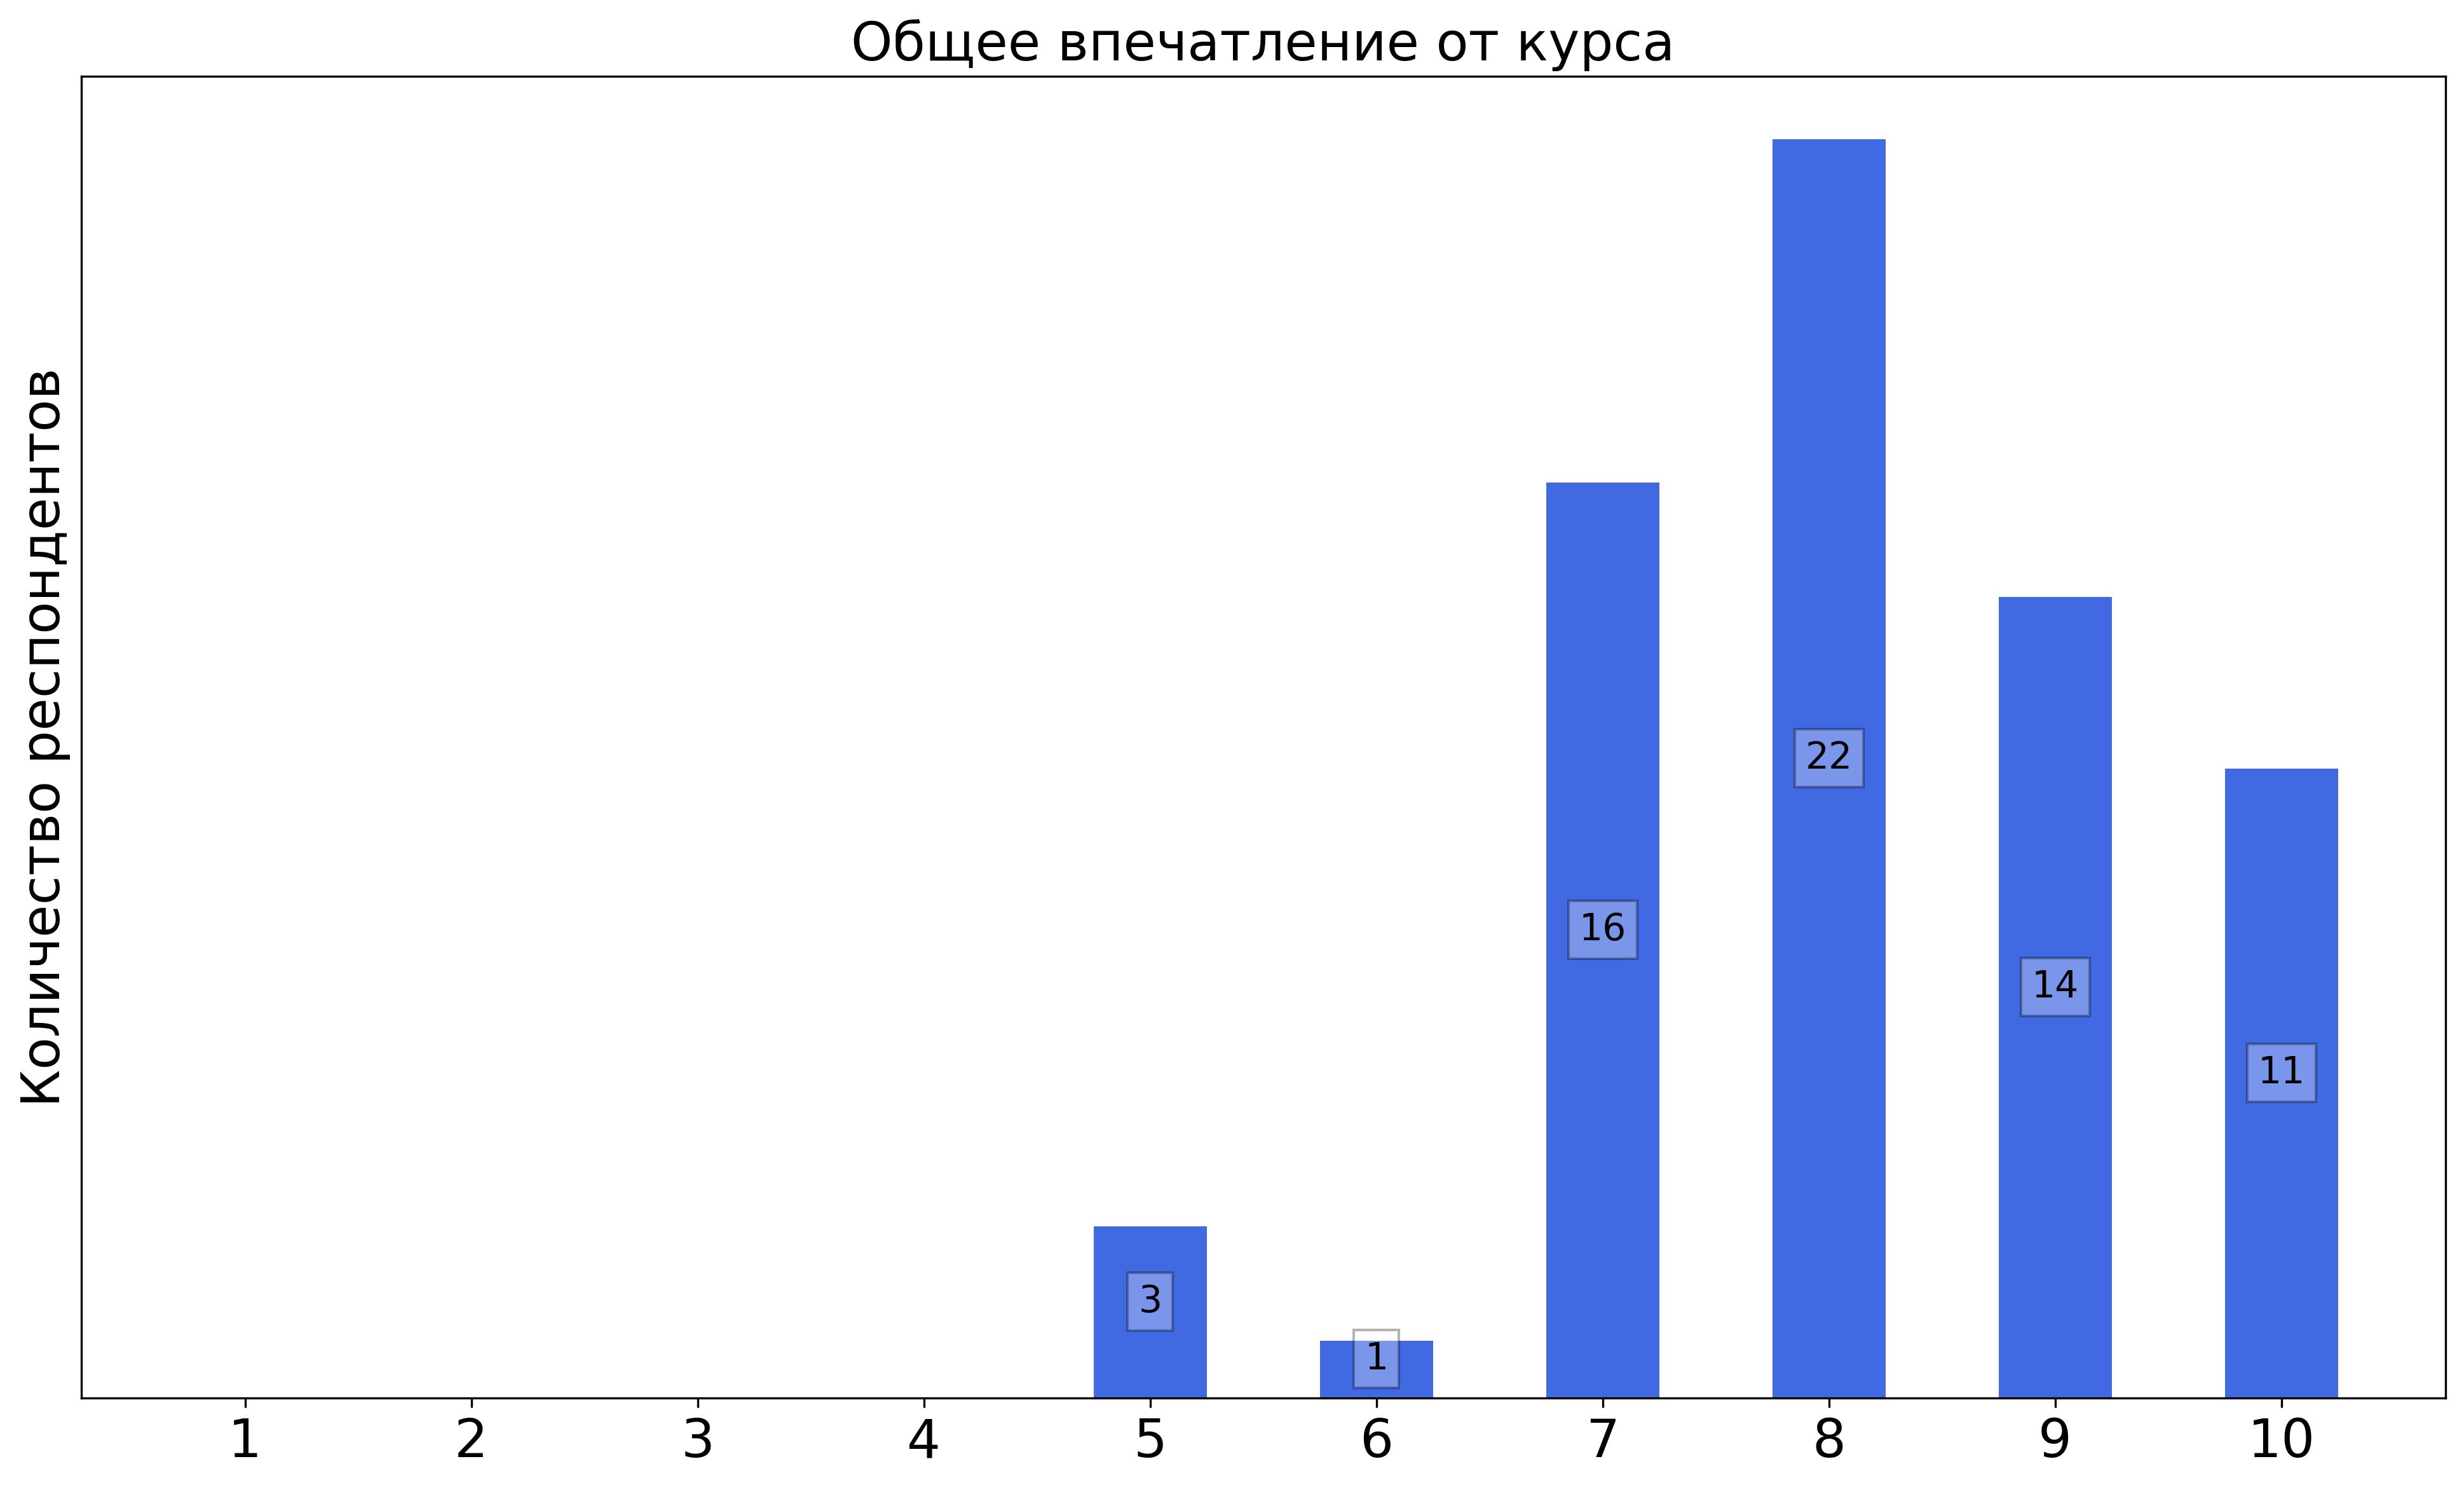
\includegraphics[width=\textwidth]{images/3 course/ТФКП/general-0.png}
			\end{subfigure}
			\begin{subfigure}[b]{0.45\textwidth}
				\centering
				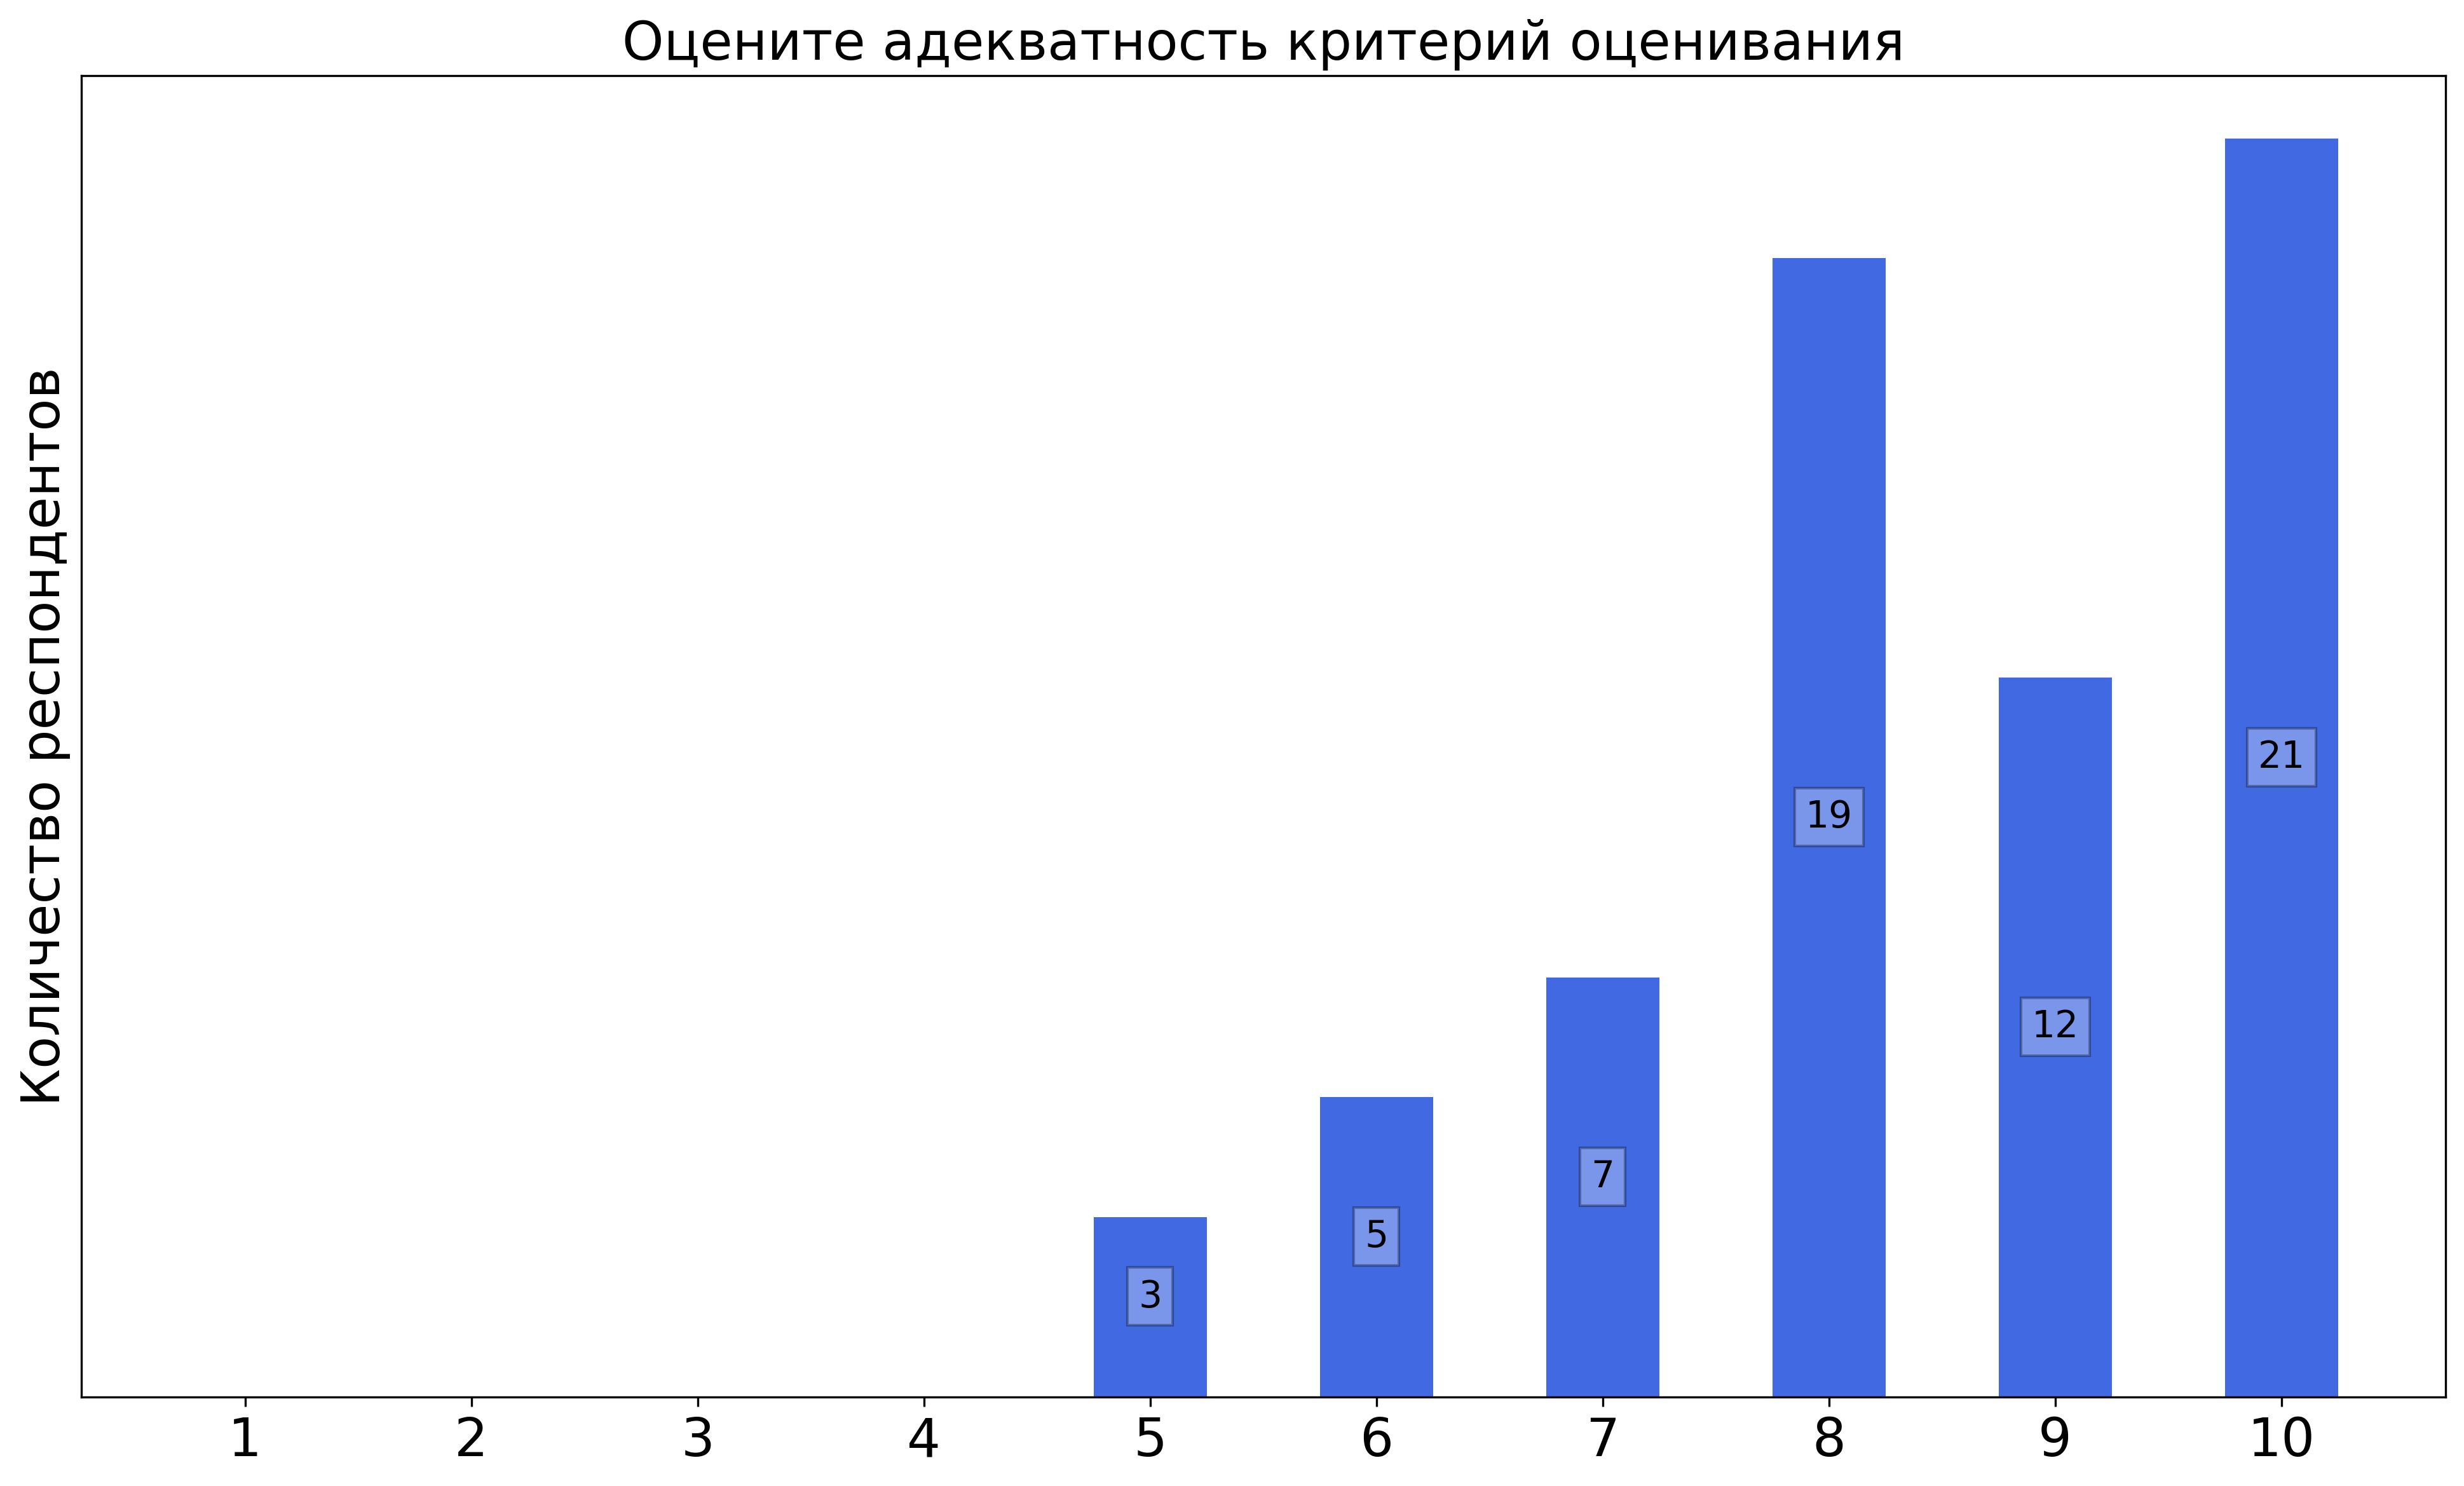
\includegraphics[width=\textwidth]{images/3 course/ТФКП/general-1.png}
			\end{subfigure}	
		\end{figure}

	\subsubsection{Материалы, использумые респондентами при изучении курса}

		\begin{figure}[H]
			\centering
			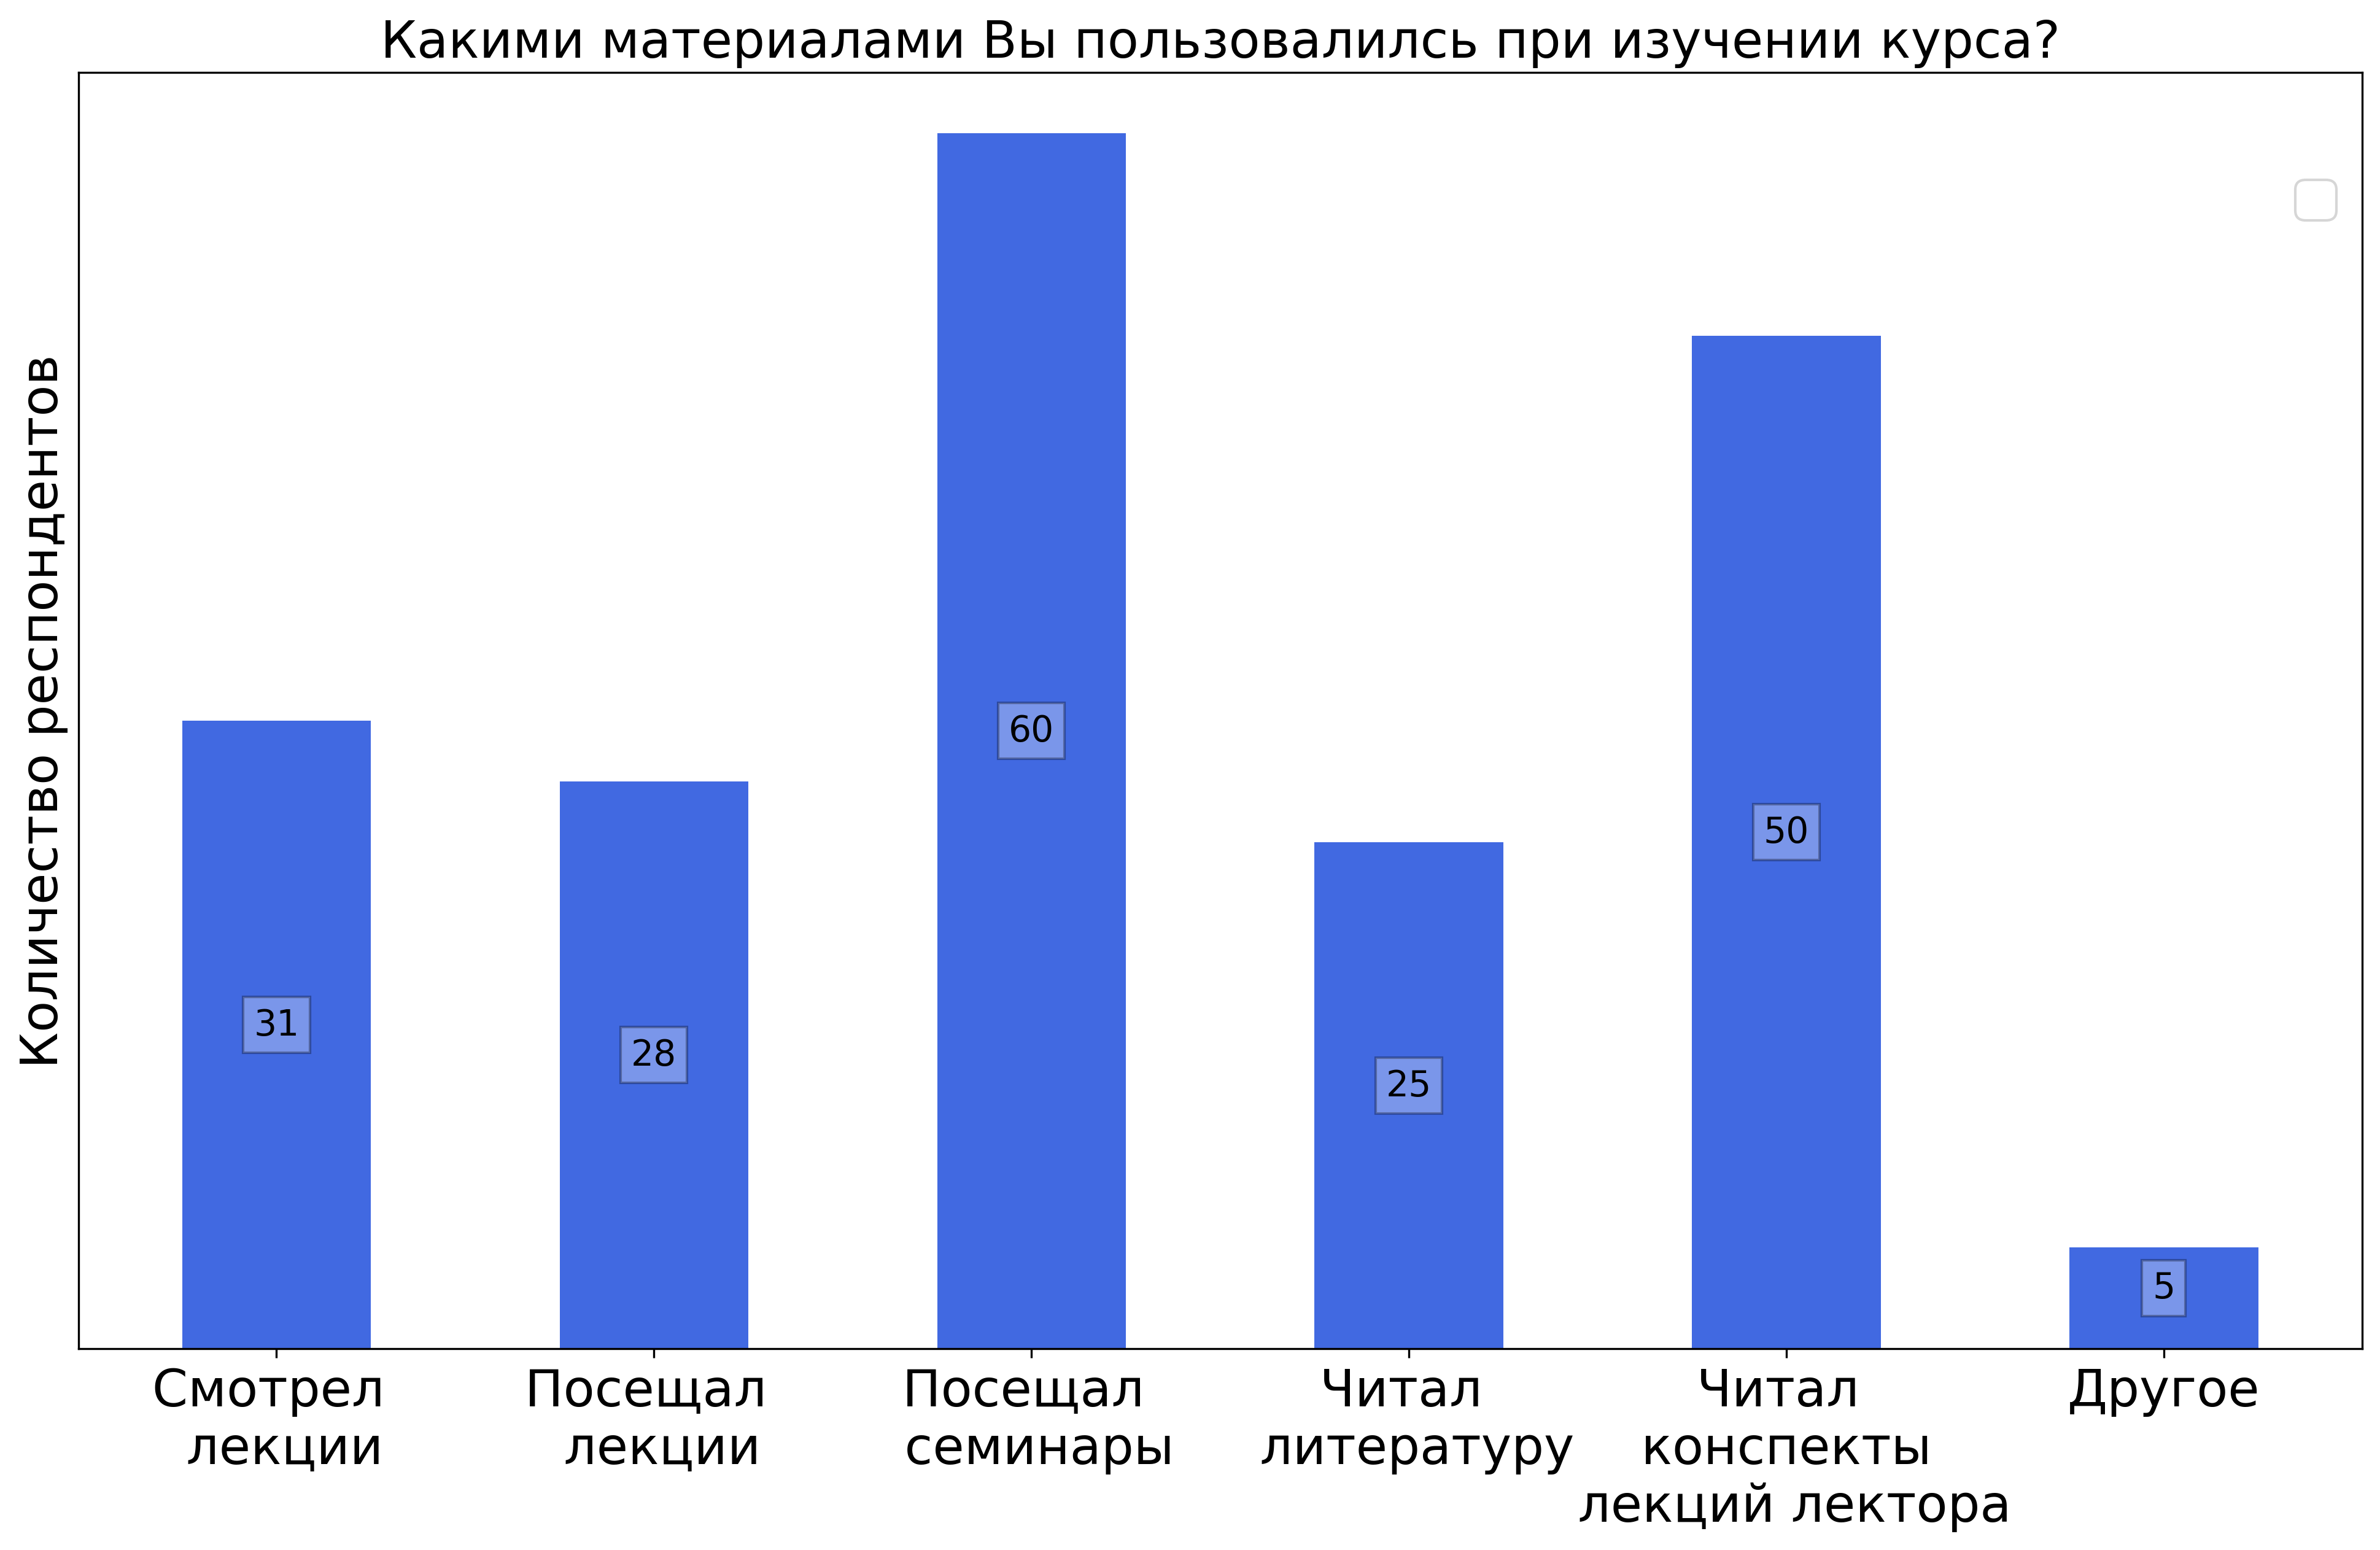
\includegraphics[width = 0.45\textwidth]{images/3 course/ТФКП/materials.png}
		\end{figure}

		\textit{В качестве других источников информации студенты указали:} 
		\begin{itemize}
			\item методички семинаристов;
			\item конспекты прошлых лет;
			\item затеханные билеты к экзамену.
		\end{itemize}

	\subsubsection{Отзыв студентов о лекциях. Лектор: Бунаков А.Э.}

		\begin{figure}[H]
			\centering
            \begin{subfigure}[b]{0.45\textwidth}
				\centering
				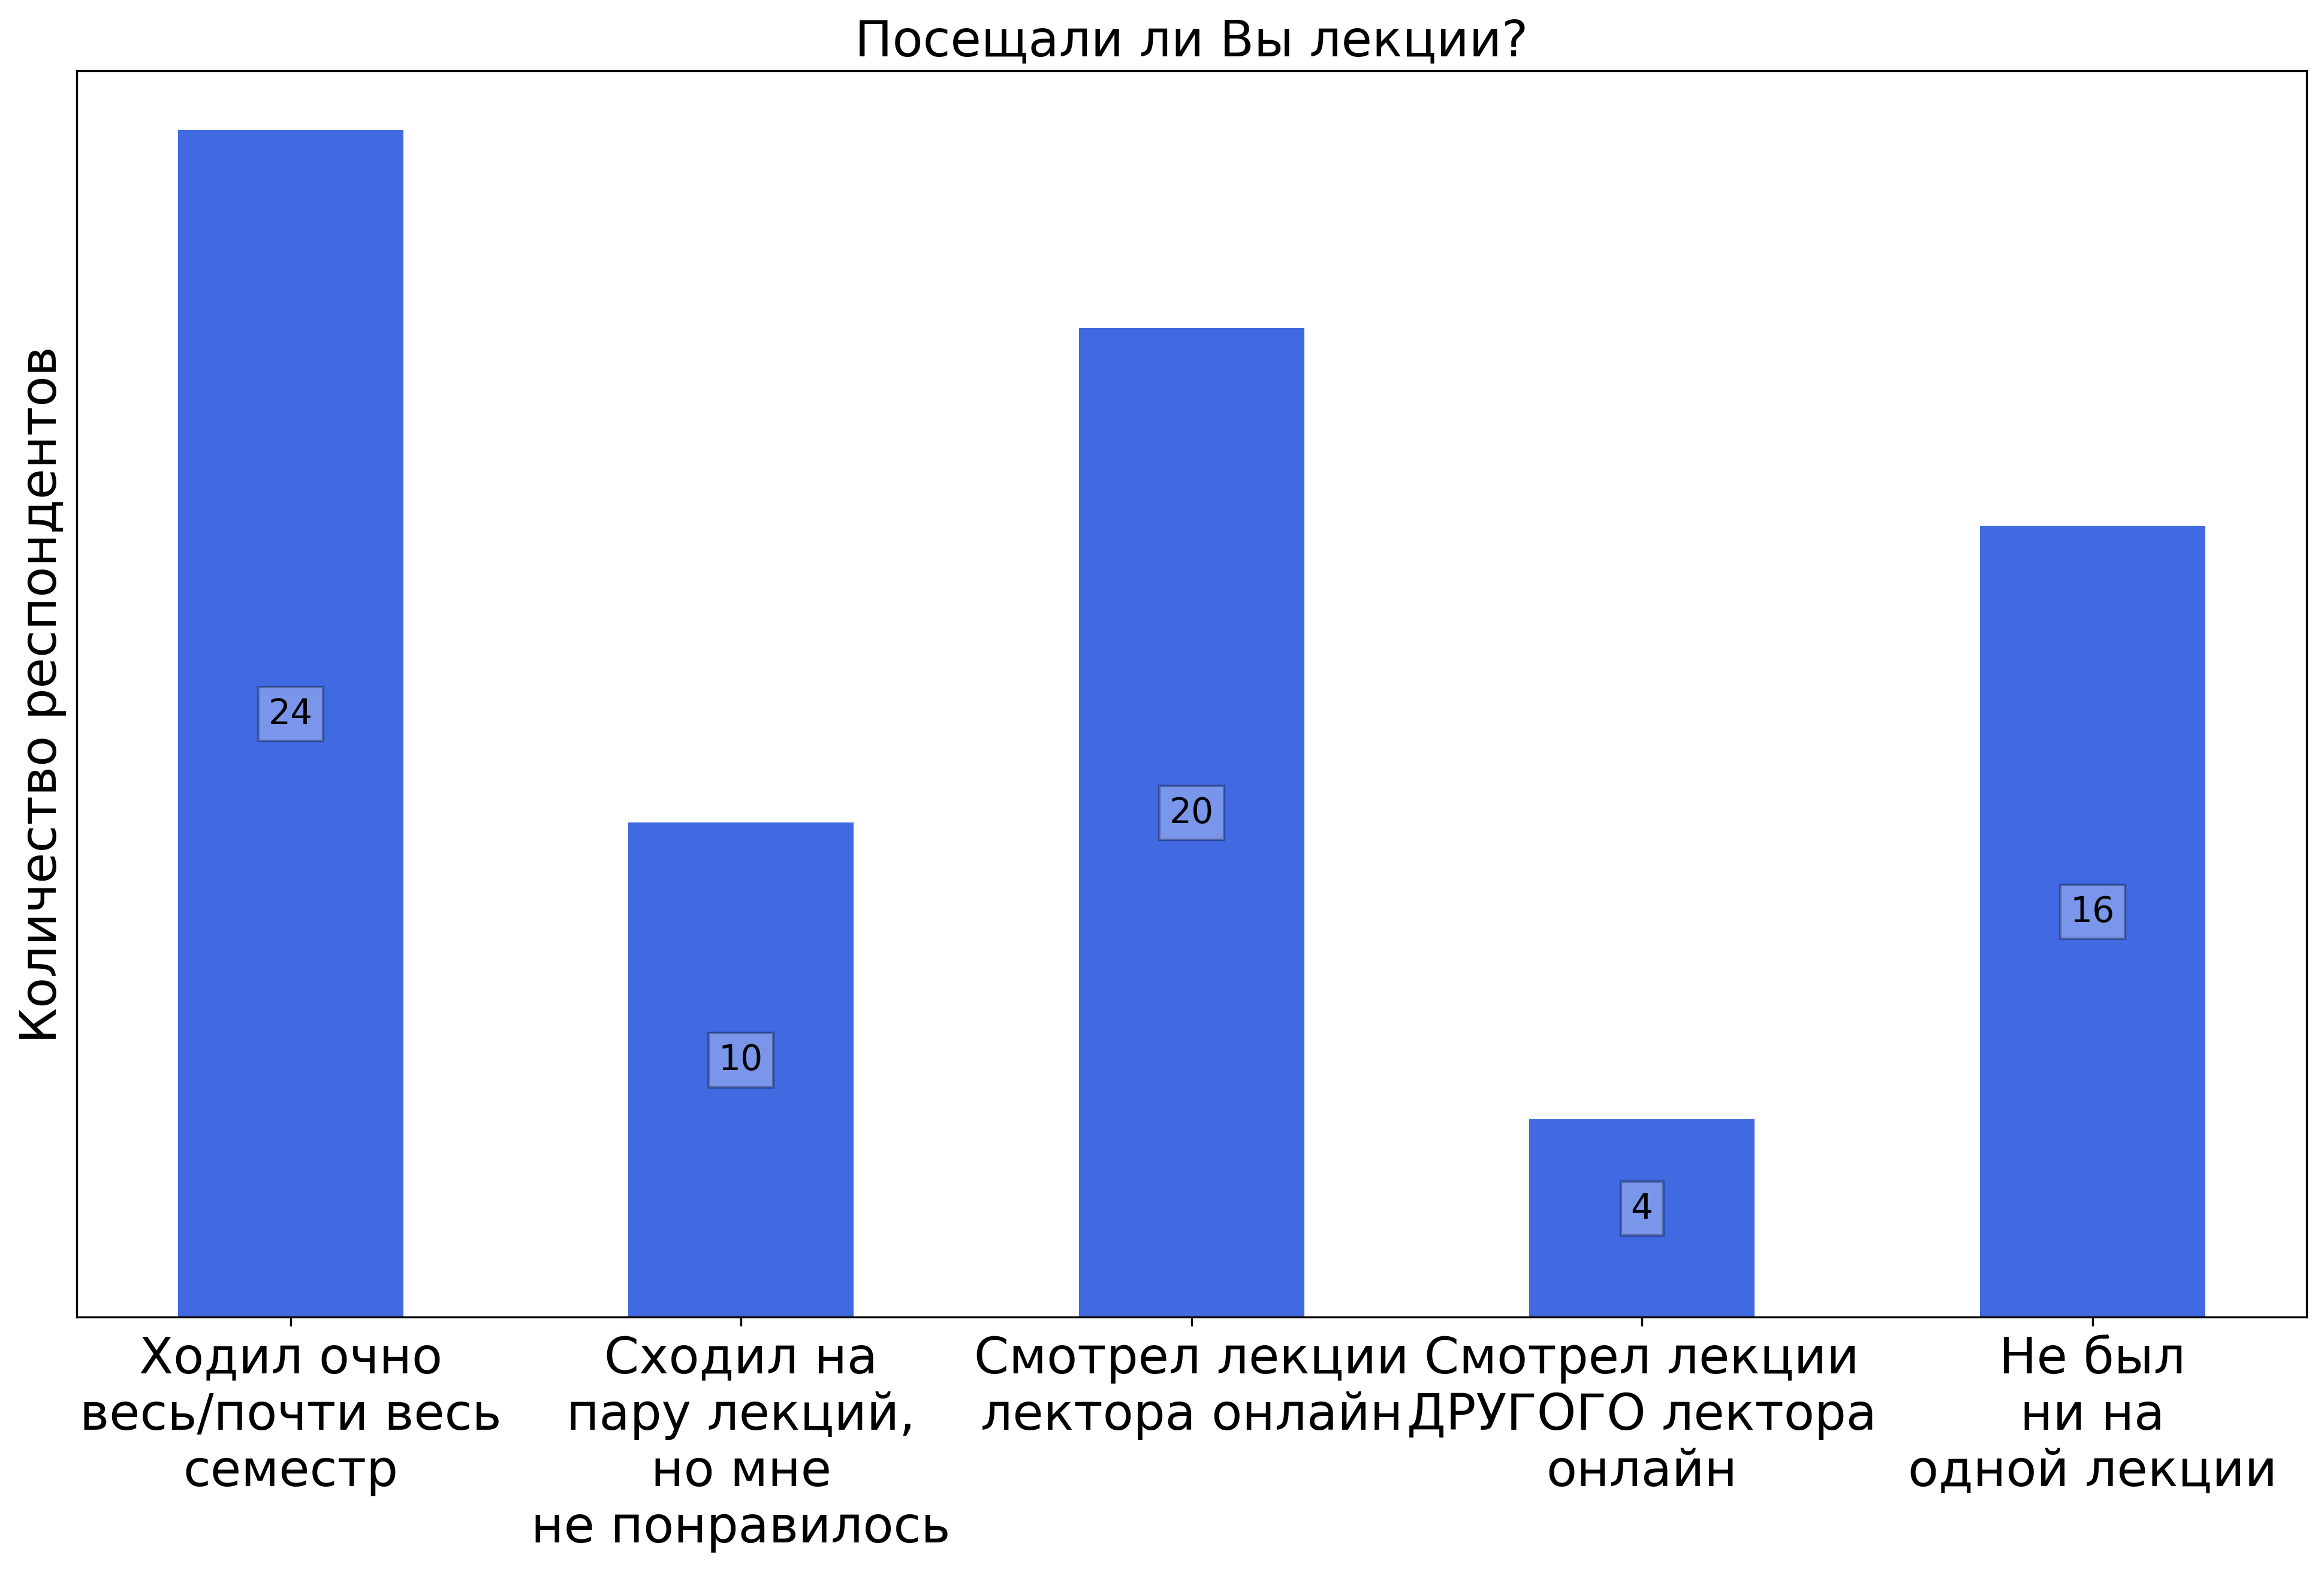
\includegraphics[width=\textwidth]{images/3 course/ТФКП/lecturer-questions-Бунаков А.Э.-0.png}
			\end{subfigure}
			\begin{subfigure}[b]{0.45\textwidth}
				\centering
				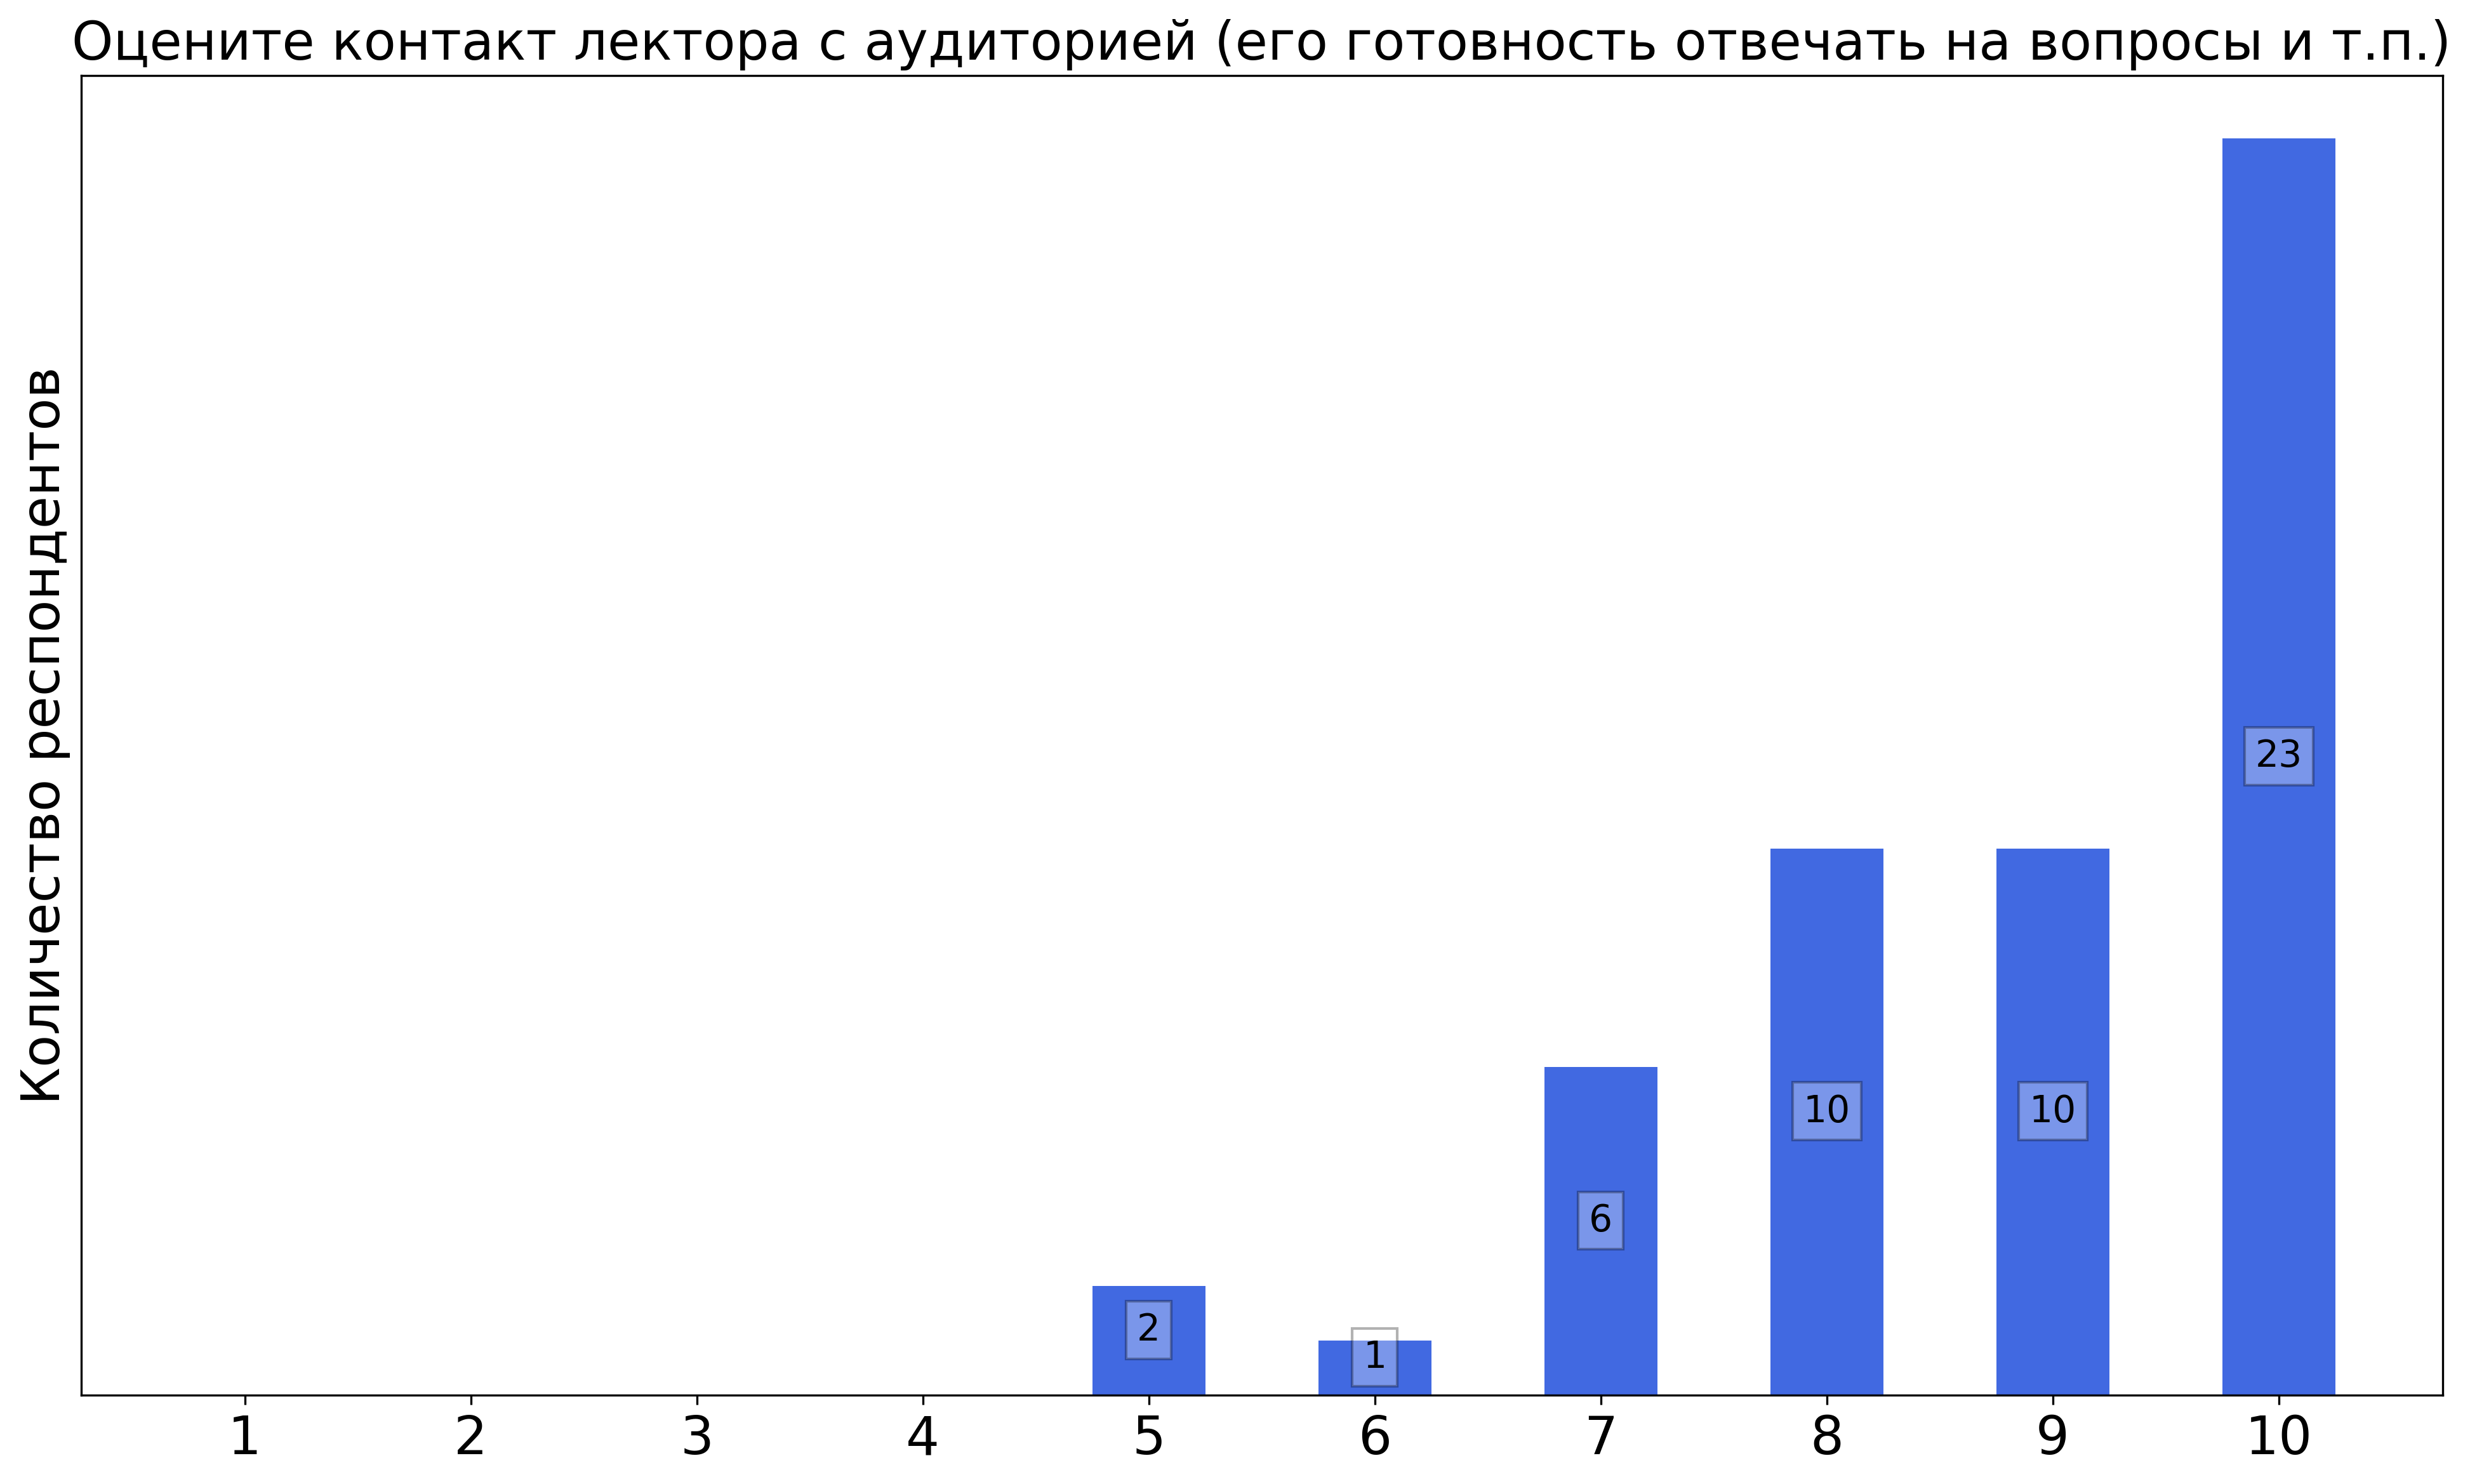
\includegraphics[width=\textwidth]{images/3 course/ТФКП/lecturer-marks-Бунаков А.Э.-0.png}
			\end{subfigure}
			\begin{subfigure}[b]{0.45\textwidth}
				\centering
				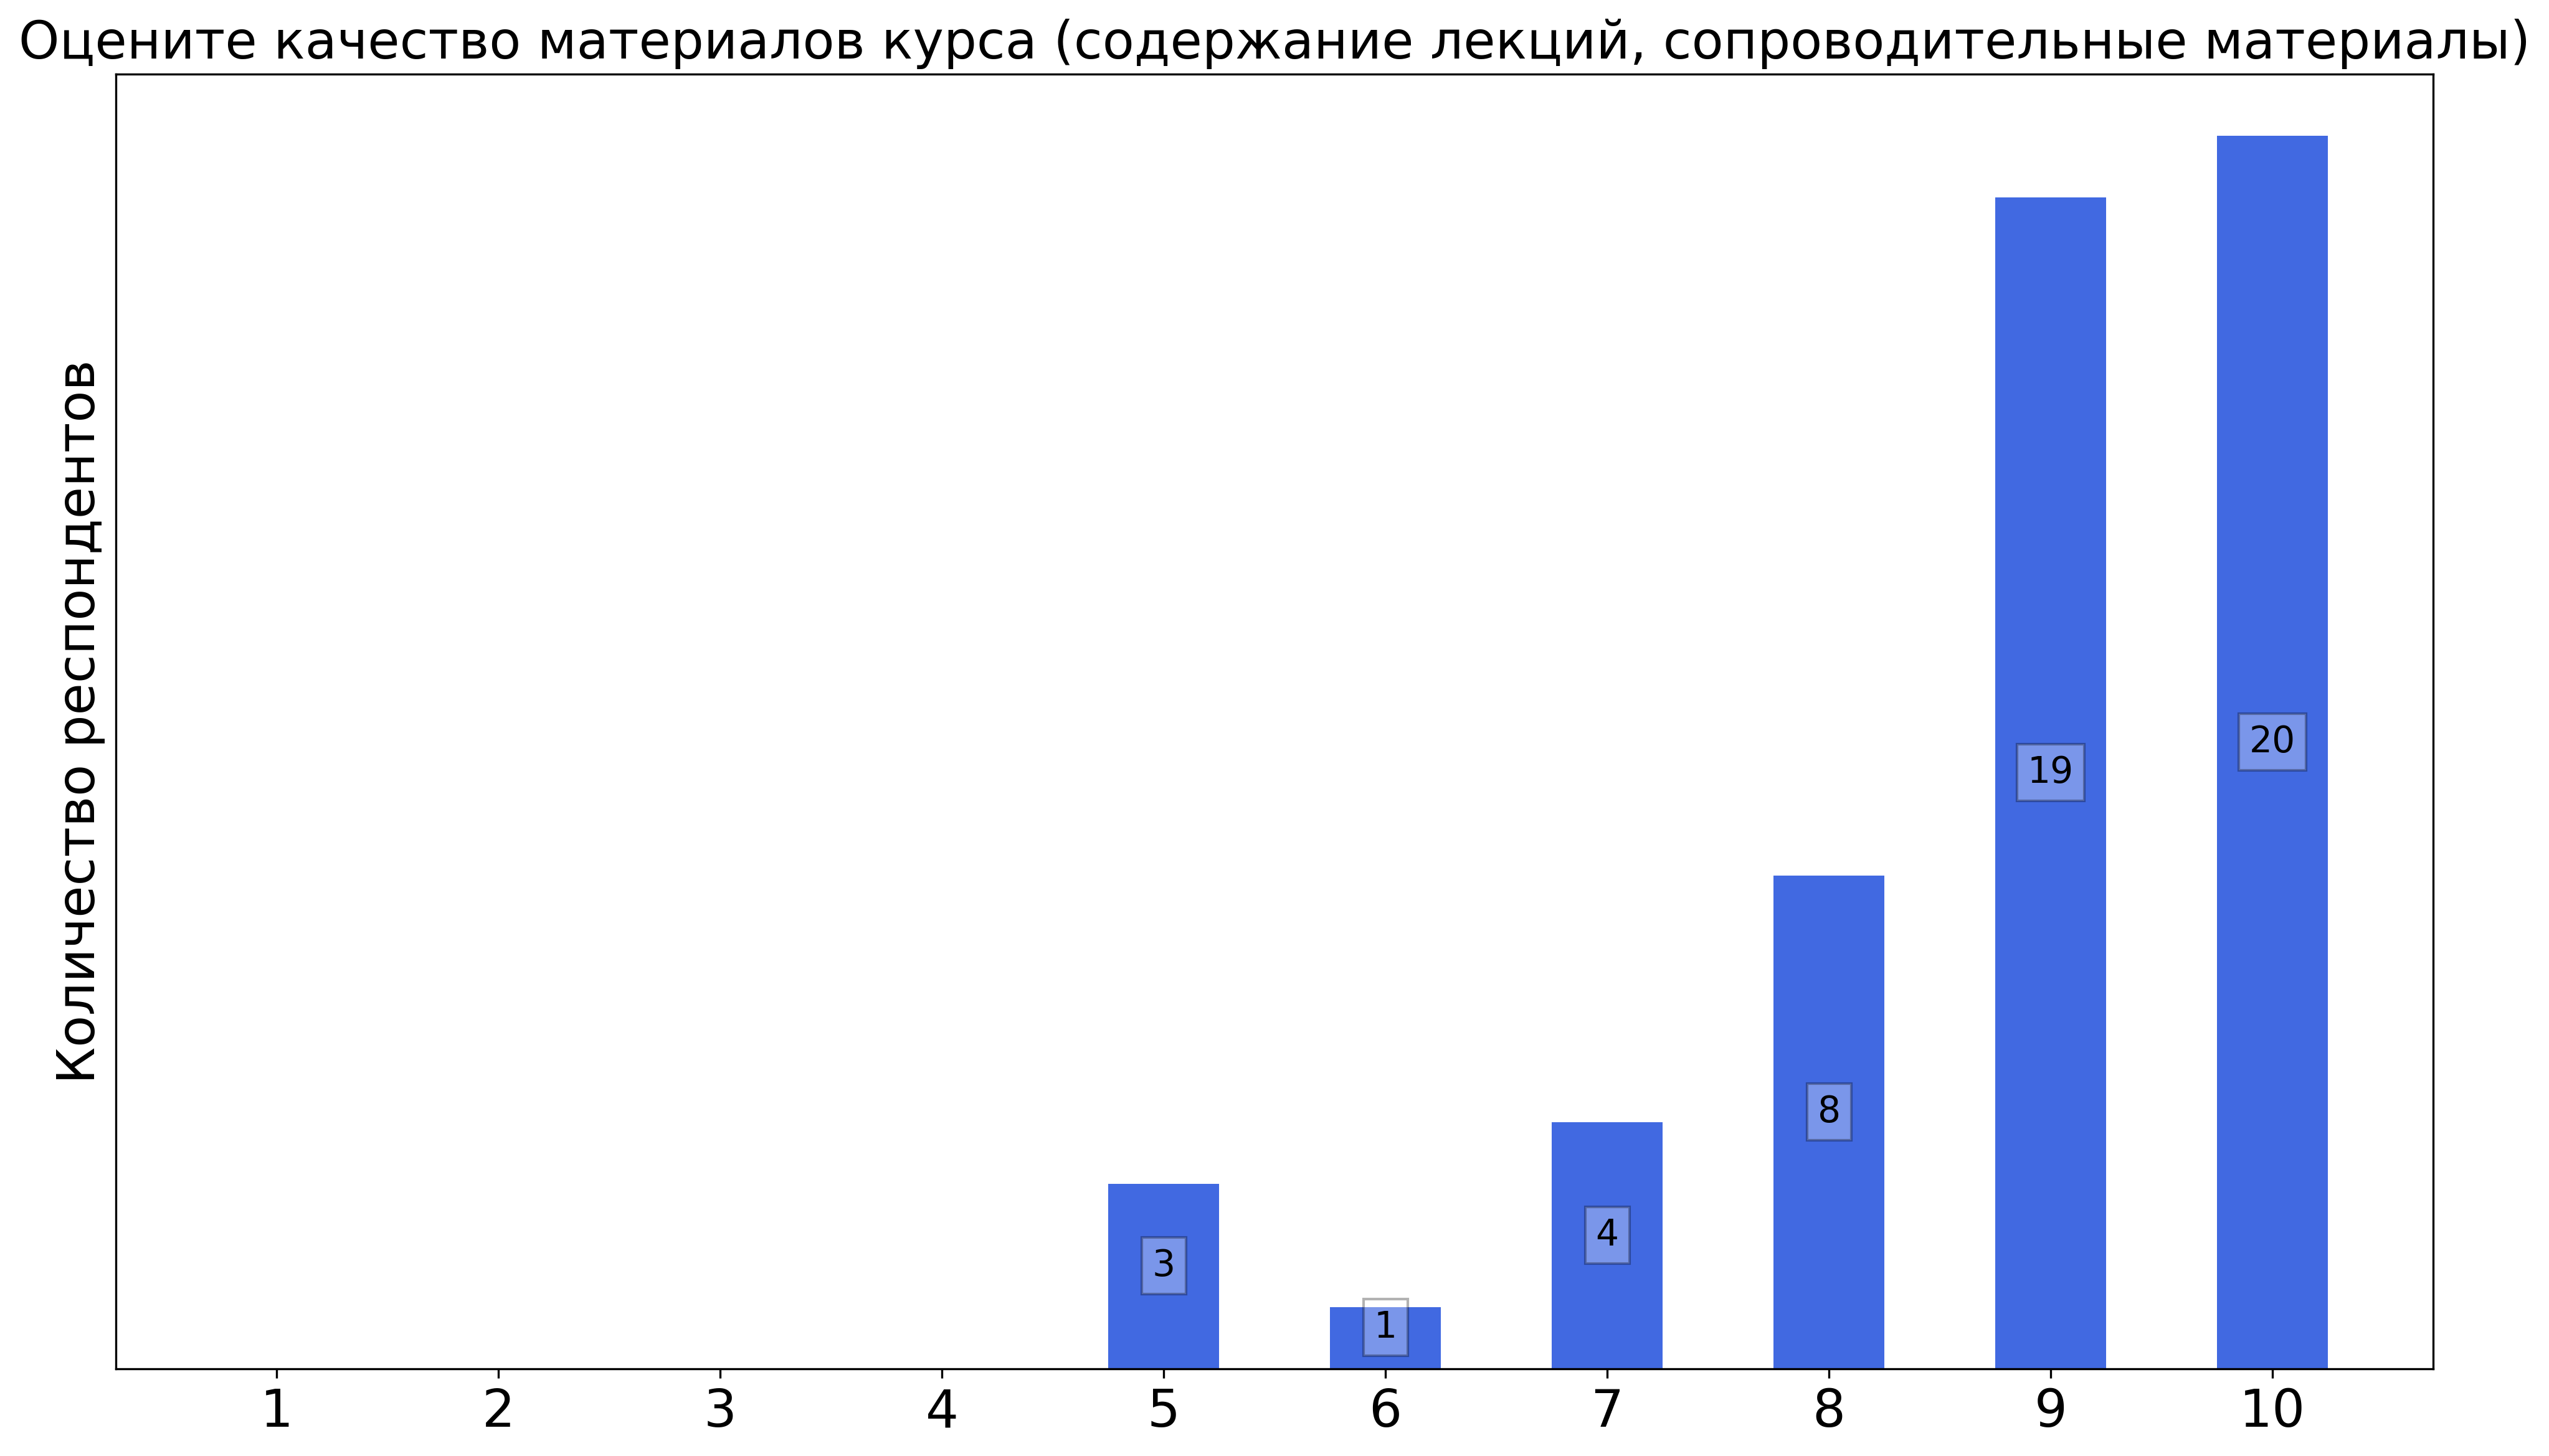
\includegraphics[width=\textwidth]{images/3 course/ТФКП/lecturer-marks-Бунаков А.Э.-1.png}
			\end{subfigure}
			\begin{subfigure}[b]{0.45\textwidth}
				\centering
				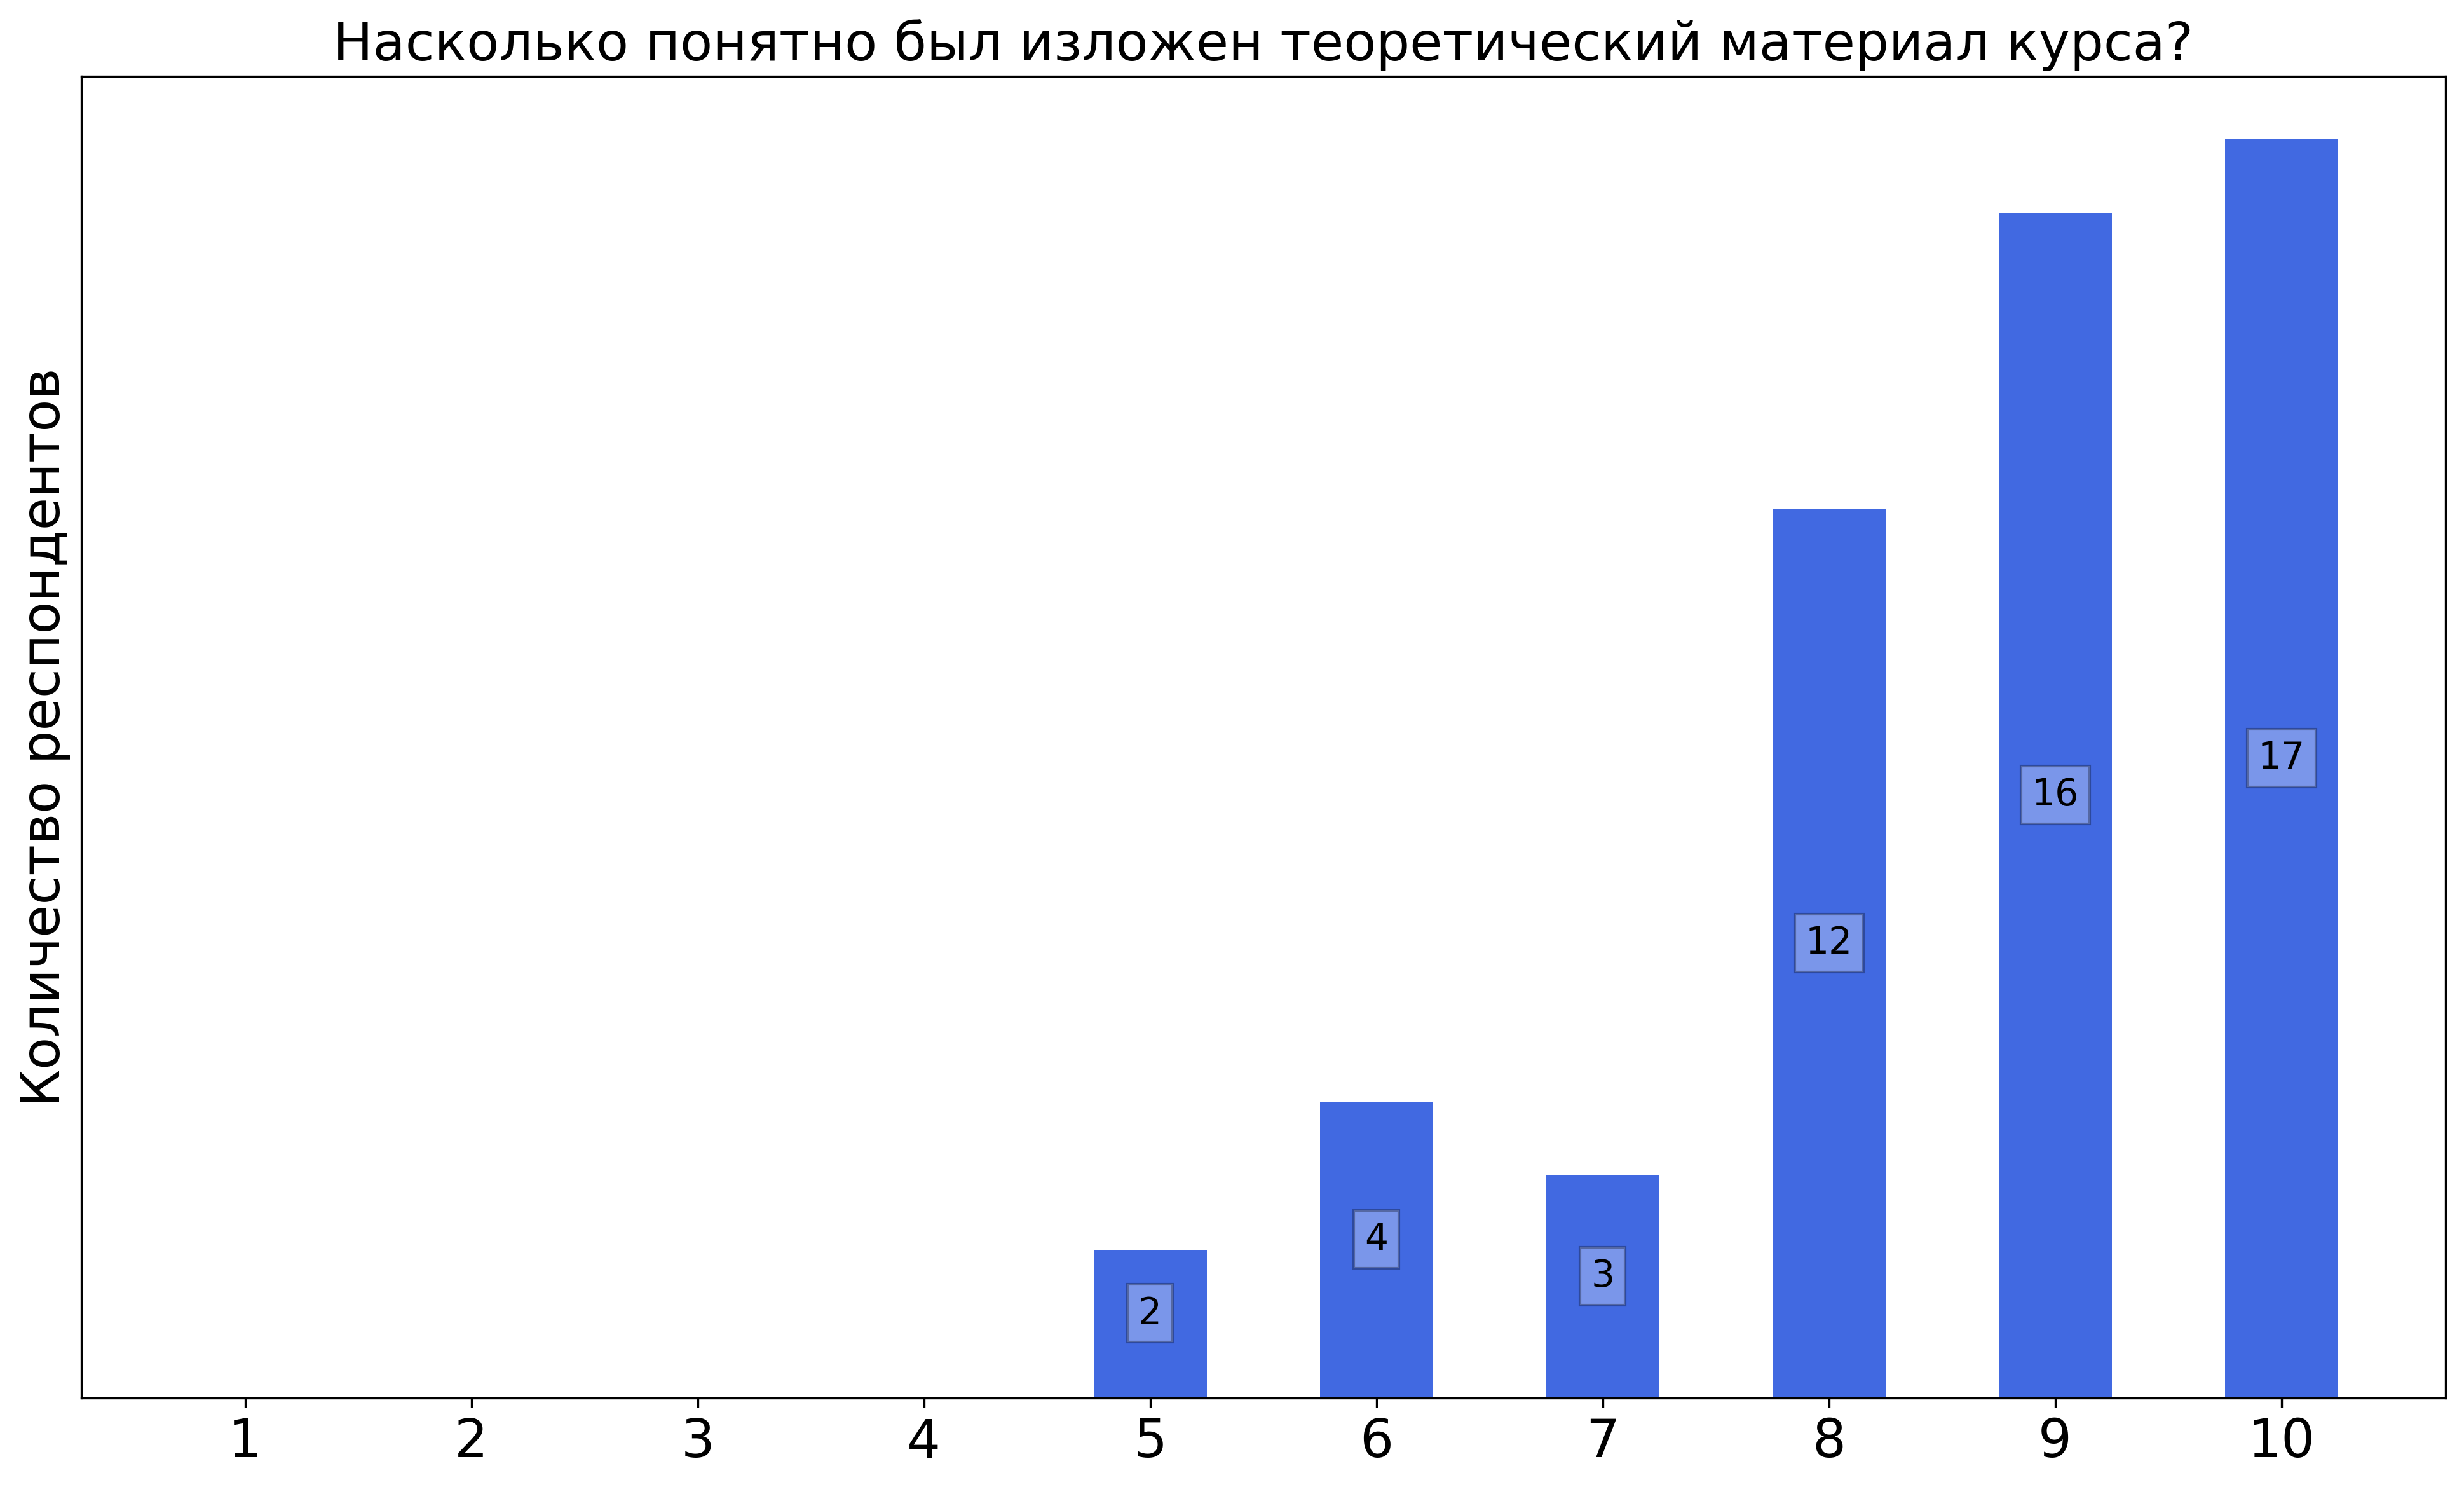
\includegraphics[width=\textwidth]{images/3 course/ТФКП/lecturer-marks-Бунаков А.Э.-2.png}
			\end{subfigure}	
			\begin{subfigure}[b]{0.45\textwidth}
				\centering
				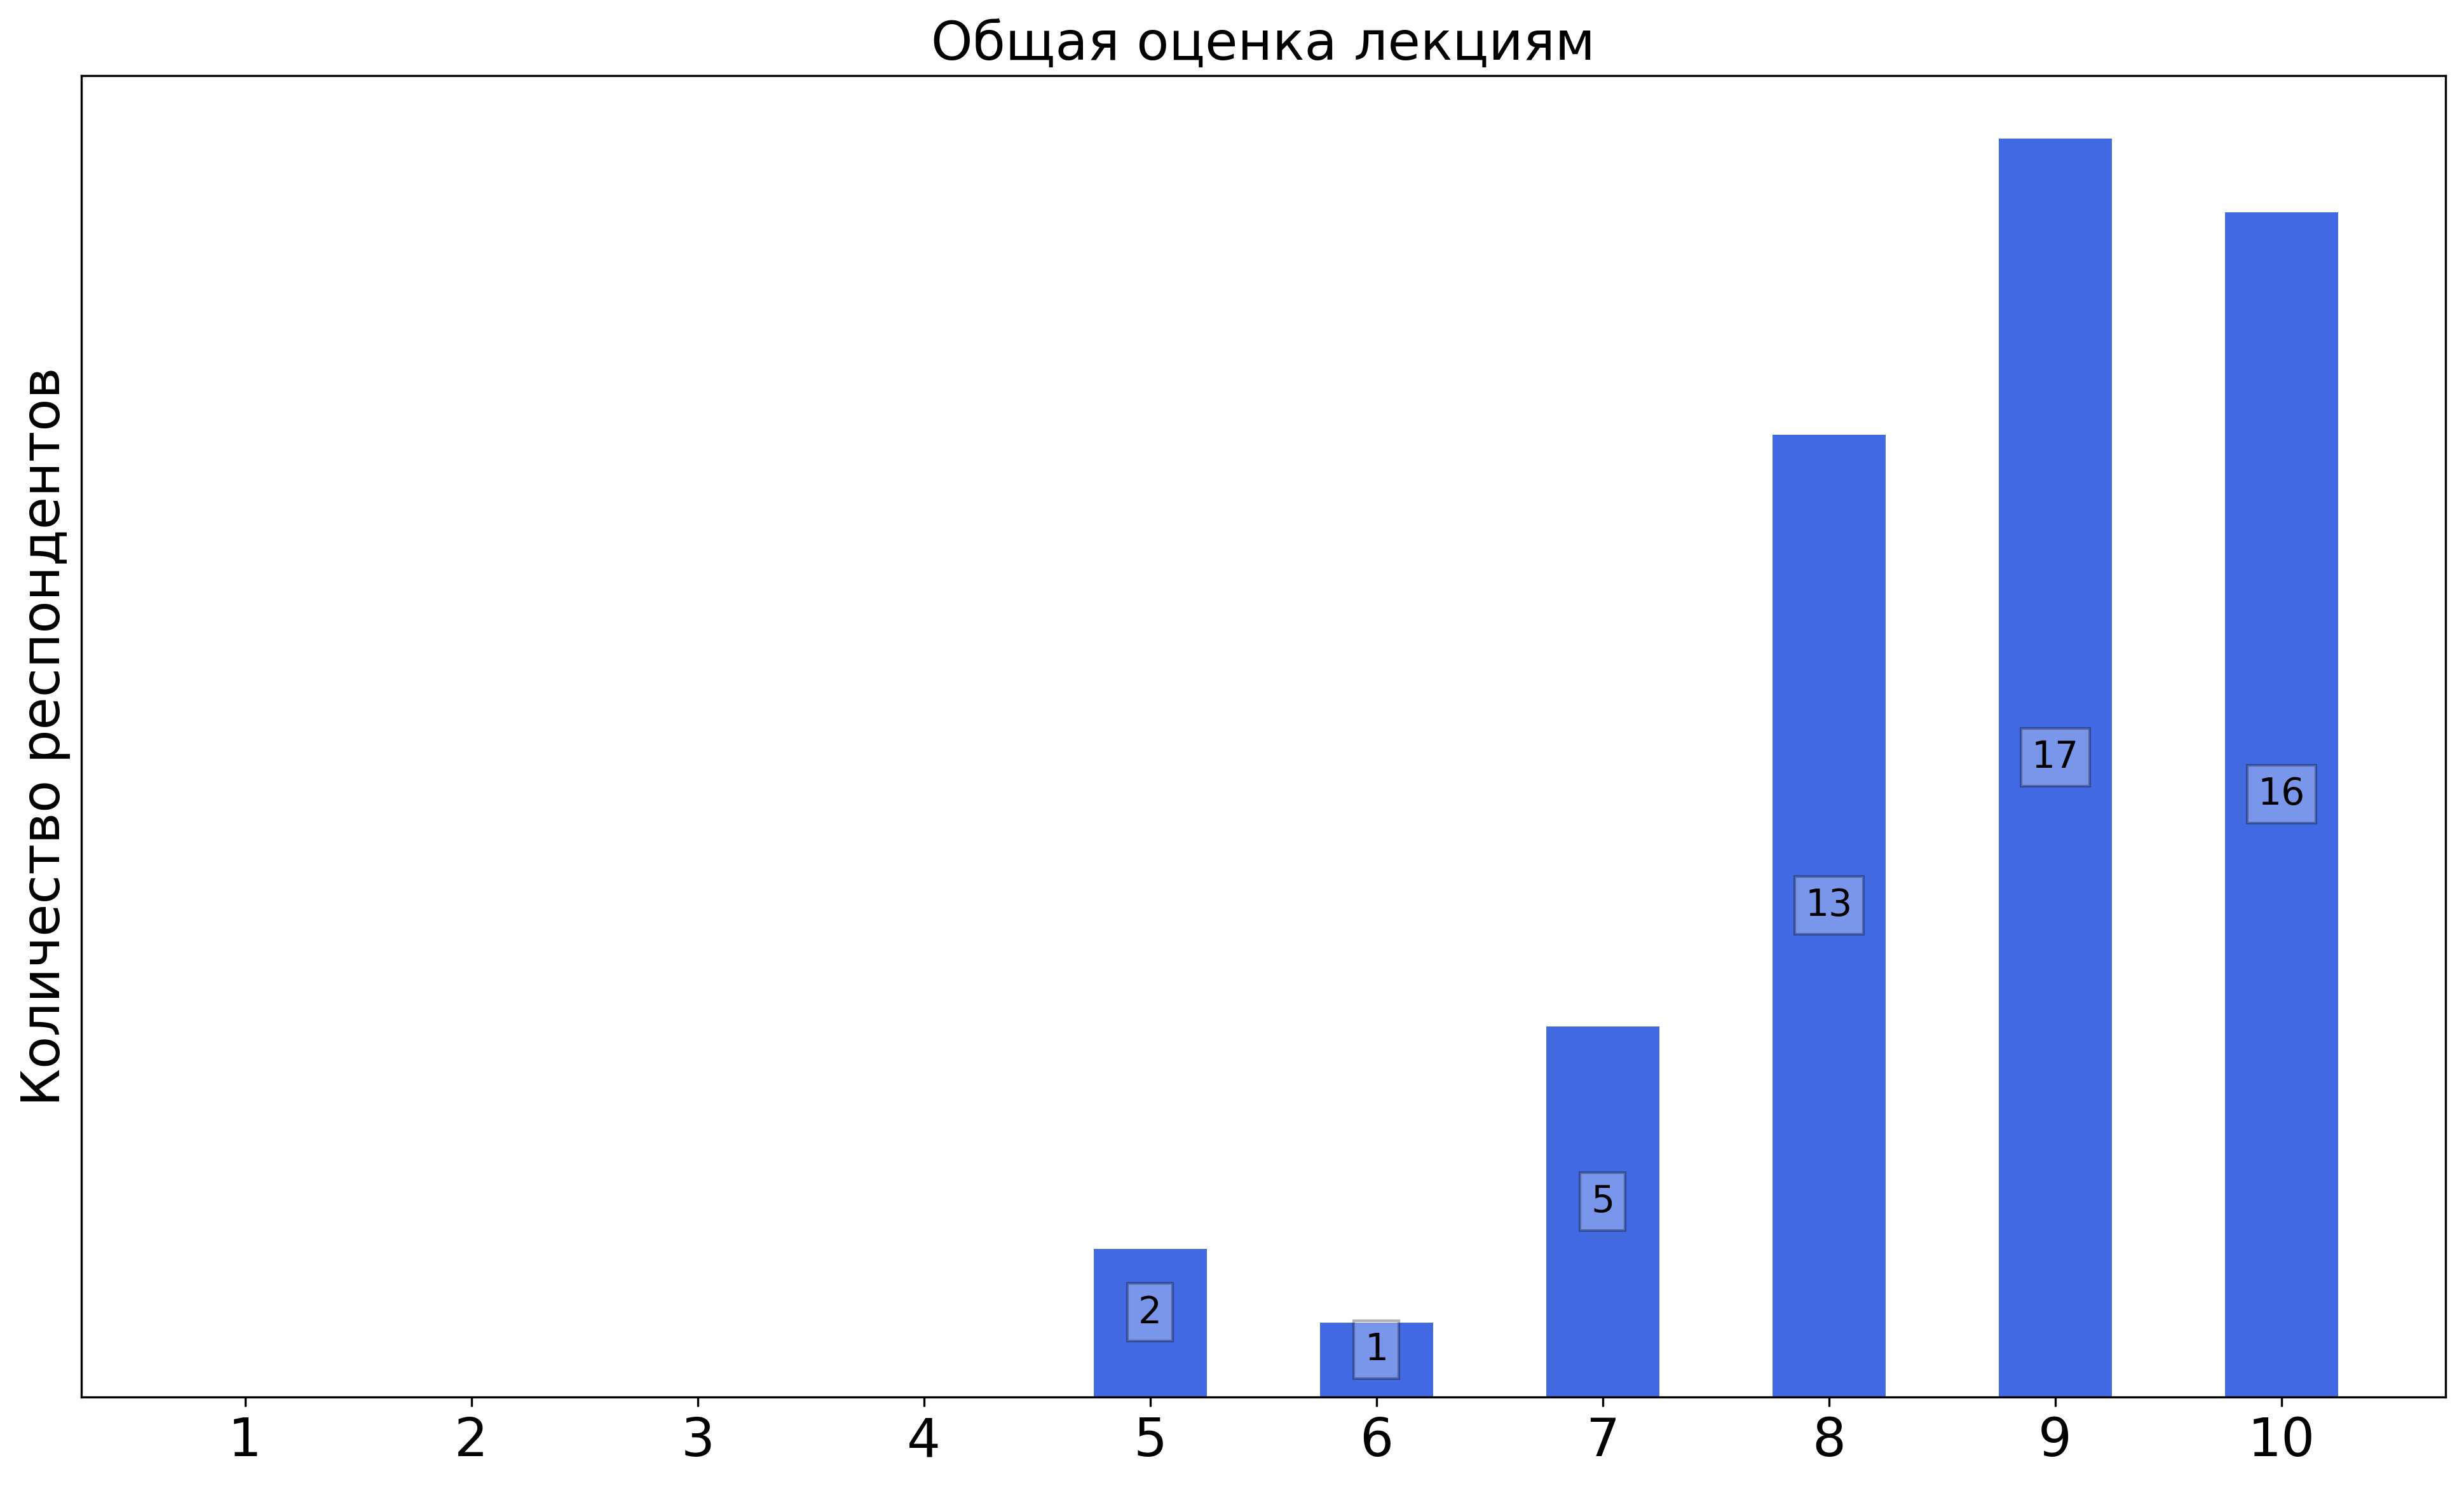
\includegraphics[width=\textwidth]{images/3 course/ТФКП/lecturer-marks-Бунаков А.Э.-3.png}
			\end{subfigure}
			\caption{Оценки респондентов о качестве преподавания лекций по курсу <<ТФКП>>}
		\end{figure}

		\textbf{Комментарии студентов о лекциях\protect\footnote{сохранены оригинальные орфография и пунктуация}}
            \begin{commentbox} 
                Лекции написаны относительно неплохо, читать их и готовиться к экзамену было неплохо по ним. Поскольку лектор вёл у меня семинары, делаю выводы, что лекции он тоже вёл хорошо 
            \end{commentbox} 
        
            \begin{commentbox} 
                Бунаков хороший ректор, все четко, структурированно 
            \end{commentbox} 
        
            \begin{commentbox} 
                Была отличная структура в лекциях, отчего было удобно конспектировать и в дальнейшем готовиться по этим конспектам 
            \end{commentbox} 
        
            \begin{commentbox} 
                В какое-то время лектор начинал читать очень быстро и рука уставала 
            \end{commentbox} 
        
            \begin{commentbox} 
                лекции в записях 2021 года отличные! 
            \end{commentbox} 
        
            \begin{commentbox} 
                Очень странно работает с доской - постоянно пишет в разных местах доски, дописывает в ограниченных им маленьких квадратиках еще незанятого полотна. Поэтому смотрелся в записи, где за рукой лектора легче проследить. А так лекции хорошие, понятные, неперегруженные 
            \end{commentbox} 
        
            \begin{commentbox} 
                Все было отлично, за исключением того, что лектор читает материал достаточно быстро, трудно бывает успевать и записывать, и понимать происходящее. Поэтому в середине семестра я перестала посещать очные лекции и стала смотреть их в записи. Материал изложен понятно, поэтому когда у меня появилась возможность ставить лектора на паузу, я без труда освоила курс 
            \end{commentbox} 
        
            \begin{commentbox} 
                Строго последовательно и главное структурировано изложен материал. Такой подход позволяет довольно быстро разобраться с программой курса. 
            \end{commentbox} 
        
            \begin{commentbox} 
                Мне понравилось. Хоть и был я на первых 3-4-х, но всё было всё хорошо. Возможно, можно было бы немного побыстрее, но это некритично.  
            \end{commentbox} 
        
            \begin{commentbox} 
                Хороший лектор, объясняет доходчиво. Единственное, немного непривычно после Знамки, что пишет не так структурировано, но это уже мелочи 
            \end{commentbox} 
        
            \begin{commentbox} 
                Бунаков - отличный лектор!  
            \end{commentbox} 
        
            \begin{commentbox} 
                Все было достаточно понятно и ёмко изложено, так что проблем не возникло. 
            \end{commentbox} 
        
            \begin{commentbox} 
                Лекции хорошие. Изложение понятное и структурированное. На все вопросы всегда отвечает 
            \end{commentbox} 
        
            \begin{commentbox} 
                Лекции проходили хорошо, лектор всегда отвечал на вопросы, если они возникали, понятно и чётко излагал материал. Слушать лекции было приятно, посетил почти на все лекции. 
            \end{commentbox} 
        
            \begin{commentbox} 
                Материал лекций изложен порядком вразнобой, поэтому было сложновато разбираться при подготовке к экзамену. 
            \end{commentbox} 
        
            \begin{commentbox} 
                Замечательный преподаватель, хорошо объясняет и доказывает теоремы. Но немного странноватая структура повествования курса. В билетах порядок теорем и тем был другой, пришлось собирать по кусочкам. 
            \end{commentbox} 
        
            \begin{commentbox} 
                Лектор хороший, всё адекватно, строго и последовательно. 
            \end{commentbox} 
        
            \begin{commentbox} 
                Хороший лектор, на вопросы отвечает охотно. Рассказывает немного нудно, слушать получается скучновато, но это матан, ничего не поделаешь. 
            \end{commentbox} 
        
            \begin{commentbox} 
                Лектор очень хорошо знает материал, не отвлекатся на посторонние разговоры 
            \end{commentbox} 
    
    

    \subsubsection{Отзыв студентов о лекциях. Лектор: Половинкин Е.С.}
        \begin{figure}[H]
            \centering
            \begin{subfigure}[b]{0.45\textwidth}
                \centering
                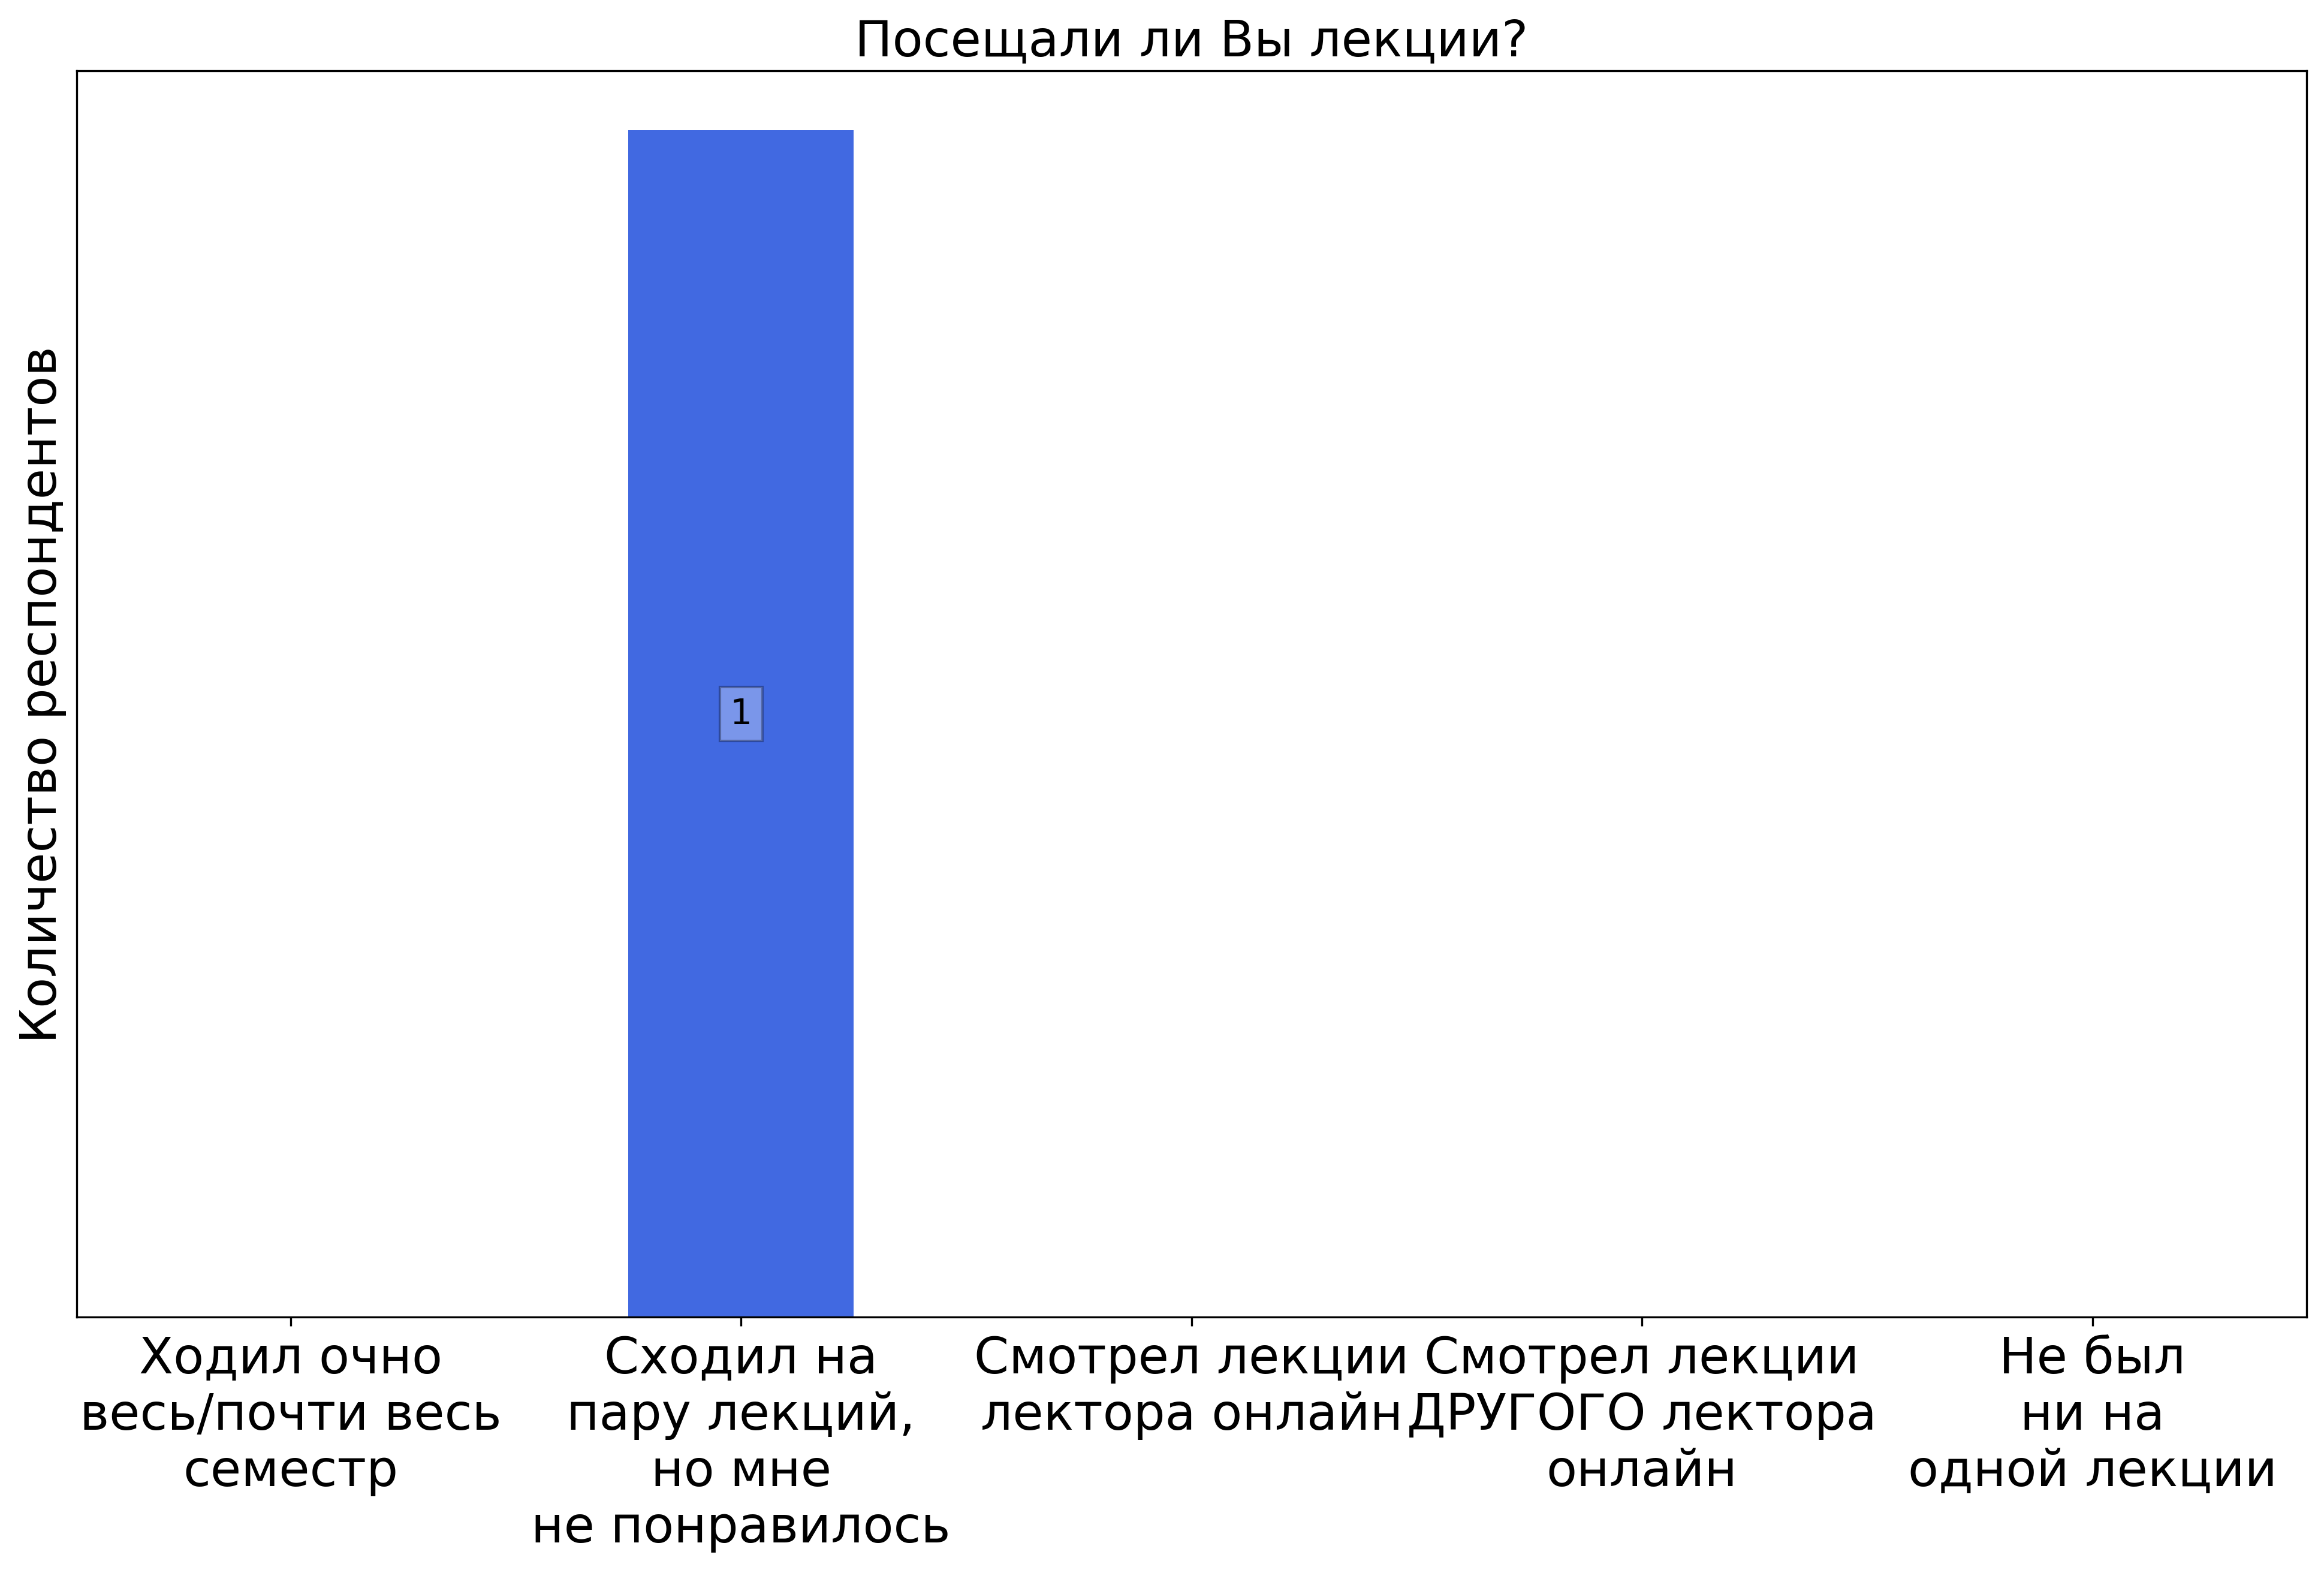
\includegraphics[width=\textwidth]{images/3 course/ТФКП/lecturer-questions-Половинкин Е.С.-0.png}
            \end{subfigure}
            \begin{subfigure}[b]{0.45\textwidth}
                \centering
                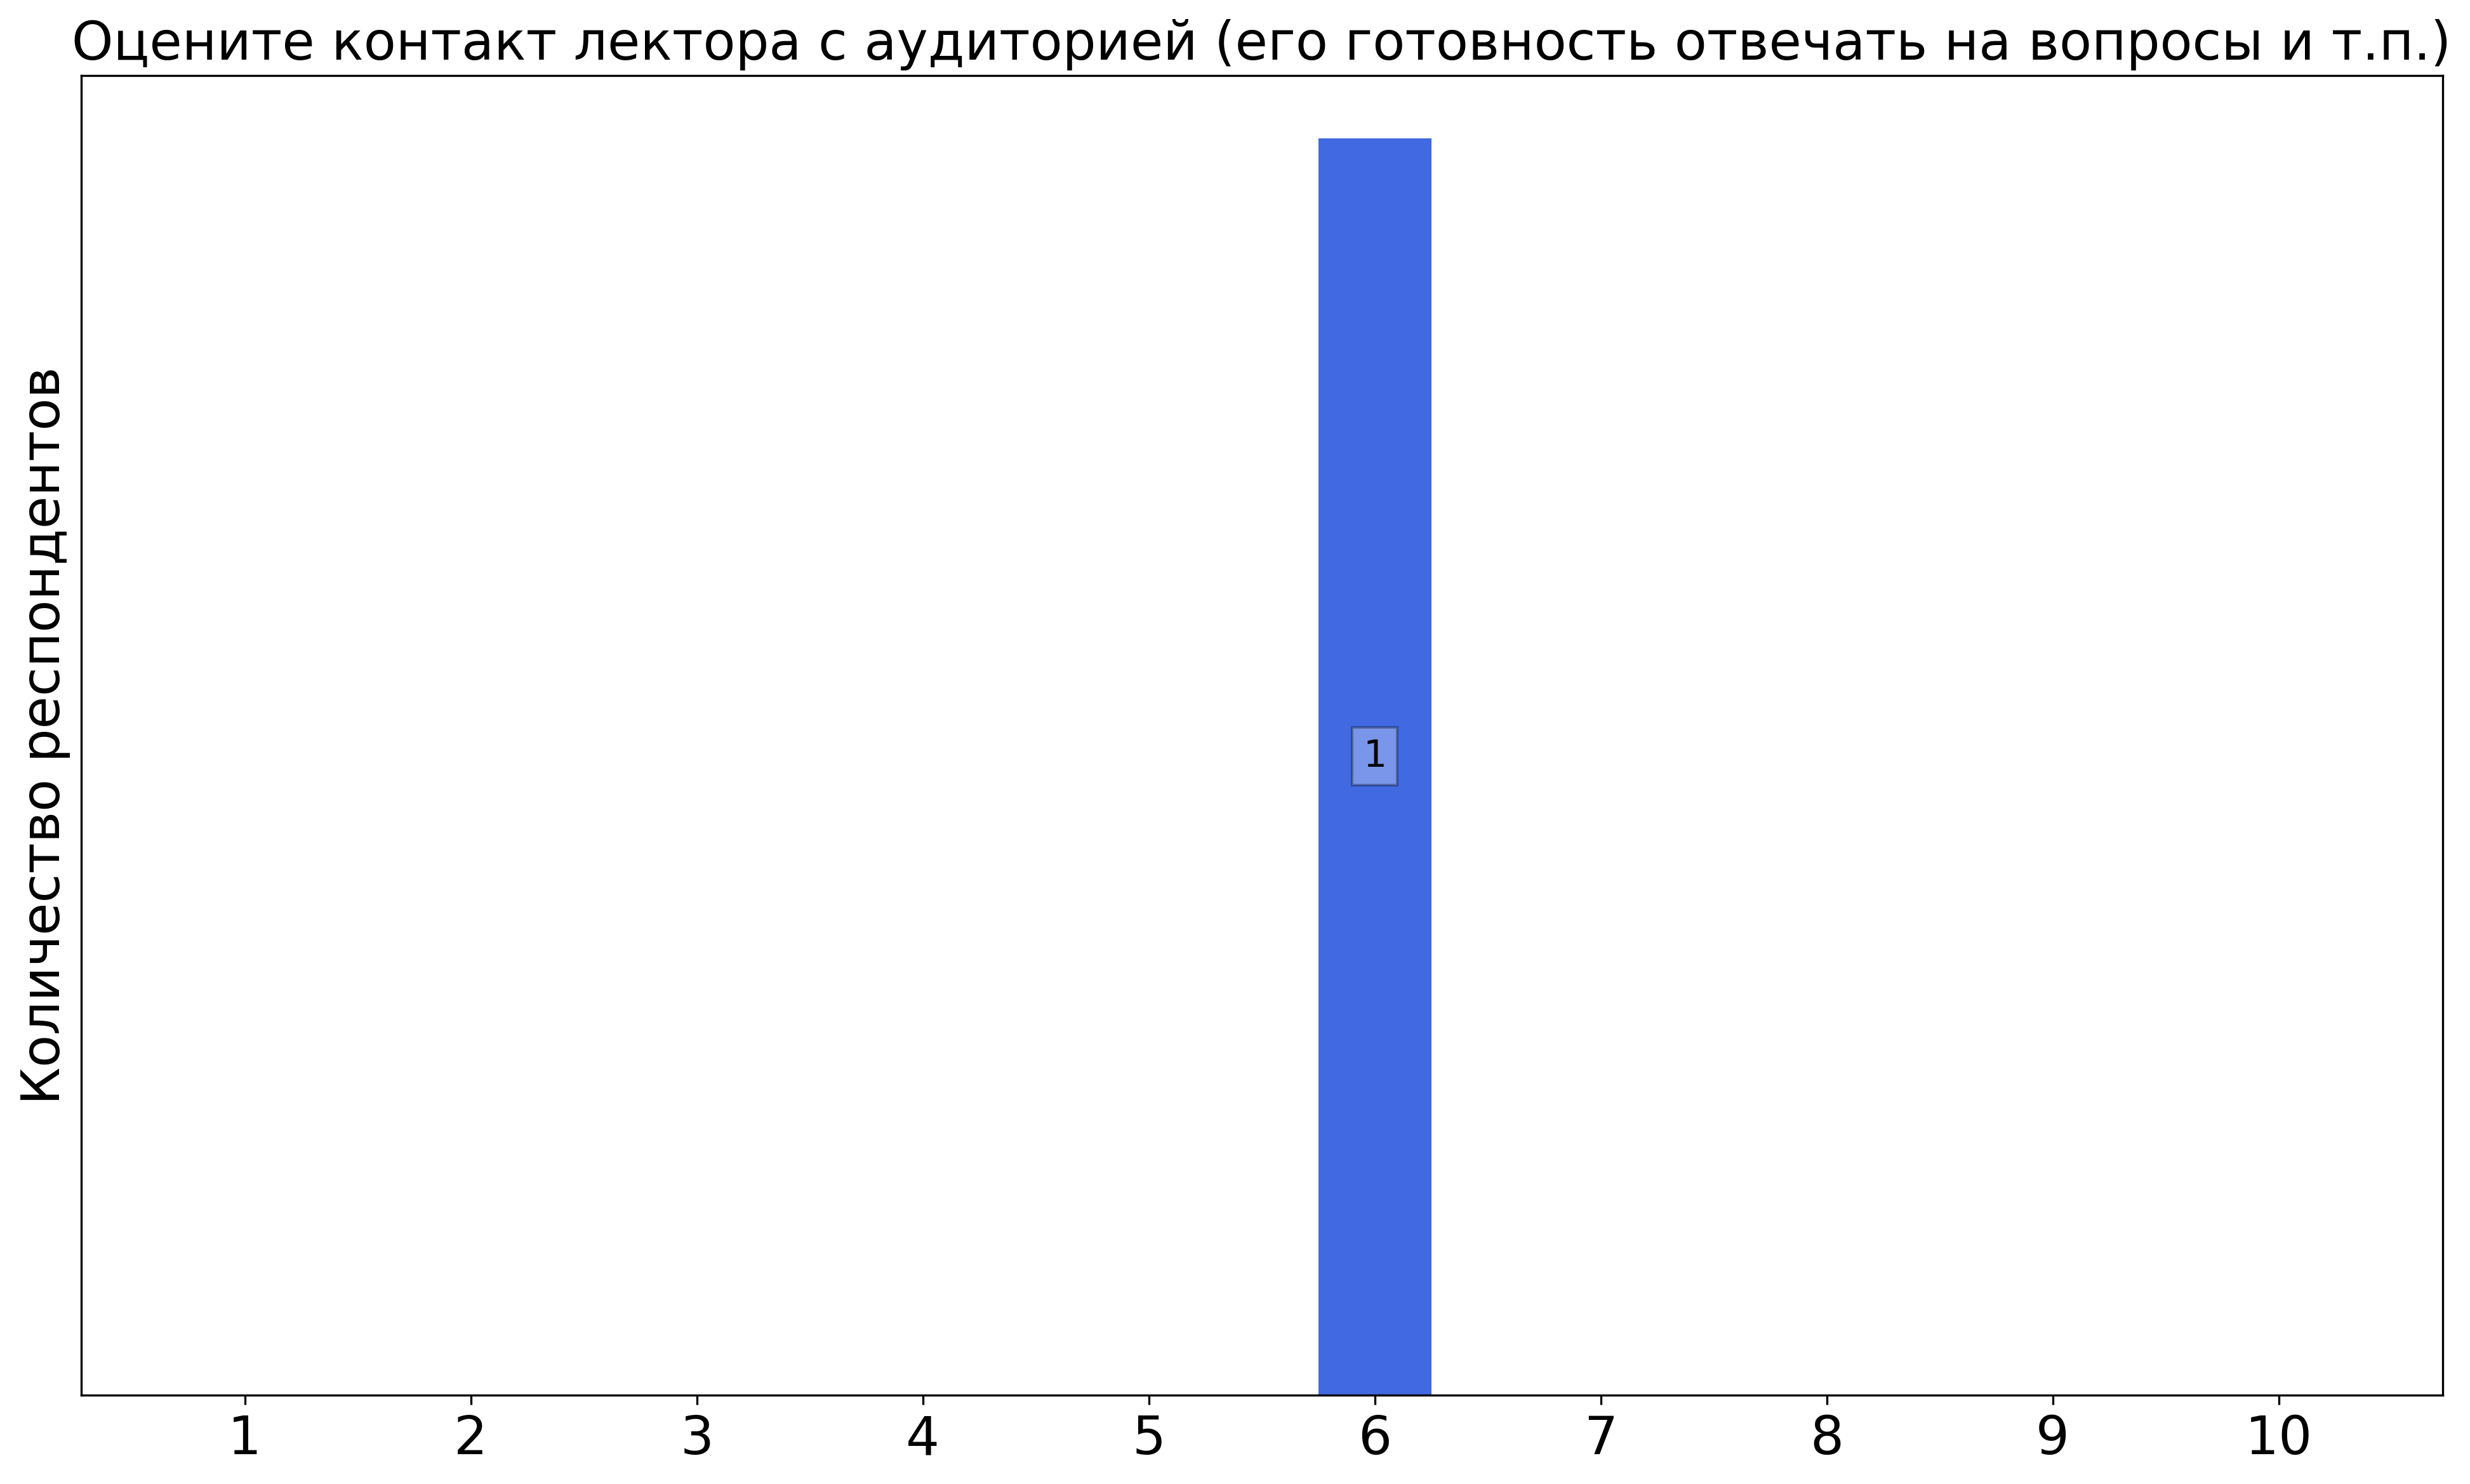
\includegraphics[width=\textwidth]{images/3 course/ТФКП/lecturer-marks-Половинкин Е.С.-0.png}
            \end{subfigure}
            \begin{subfigure}[b]{0.45\textwidth}
                \centering
                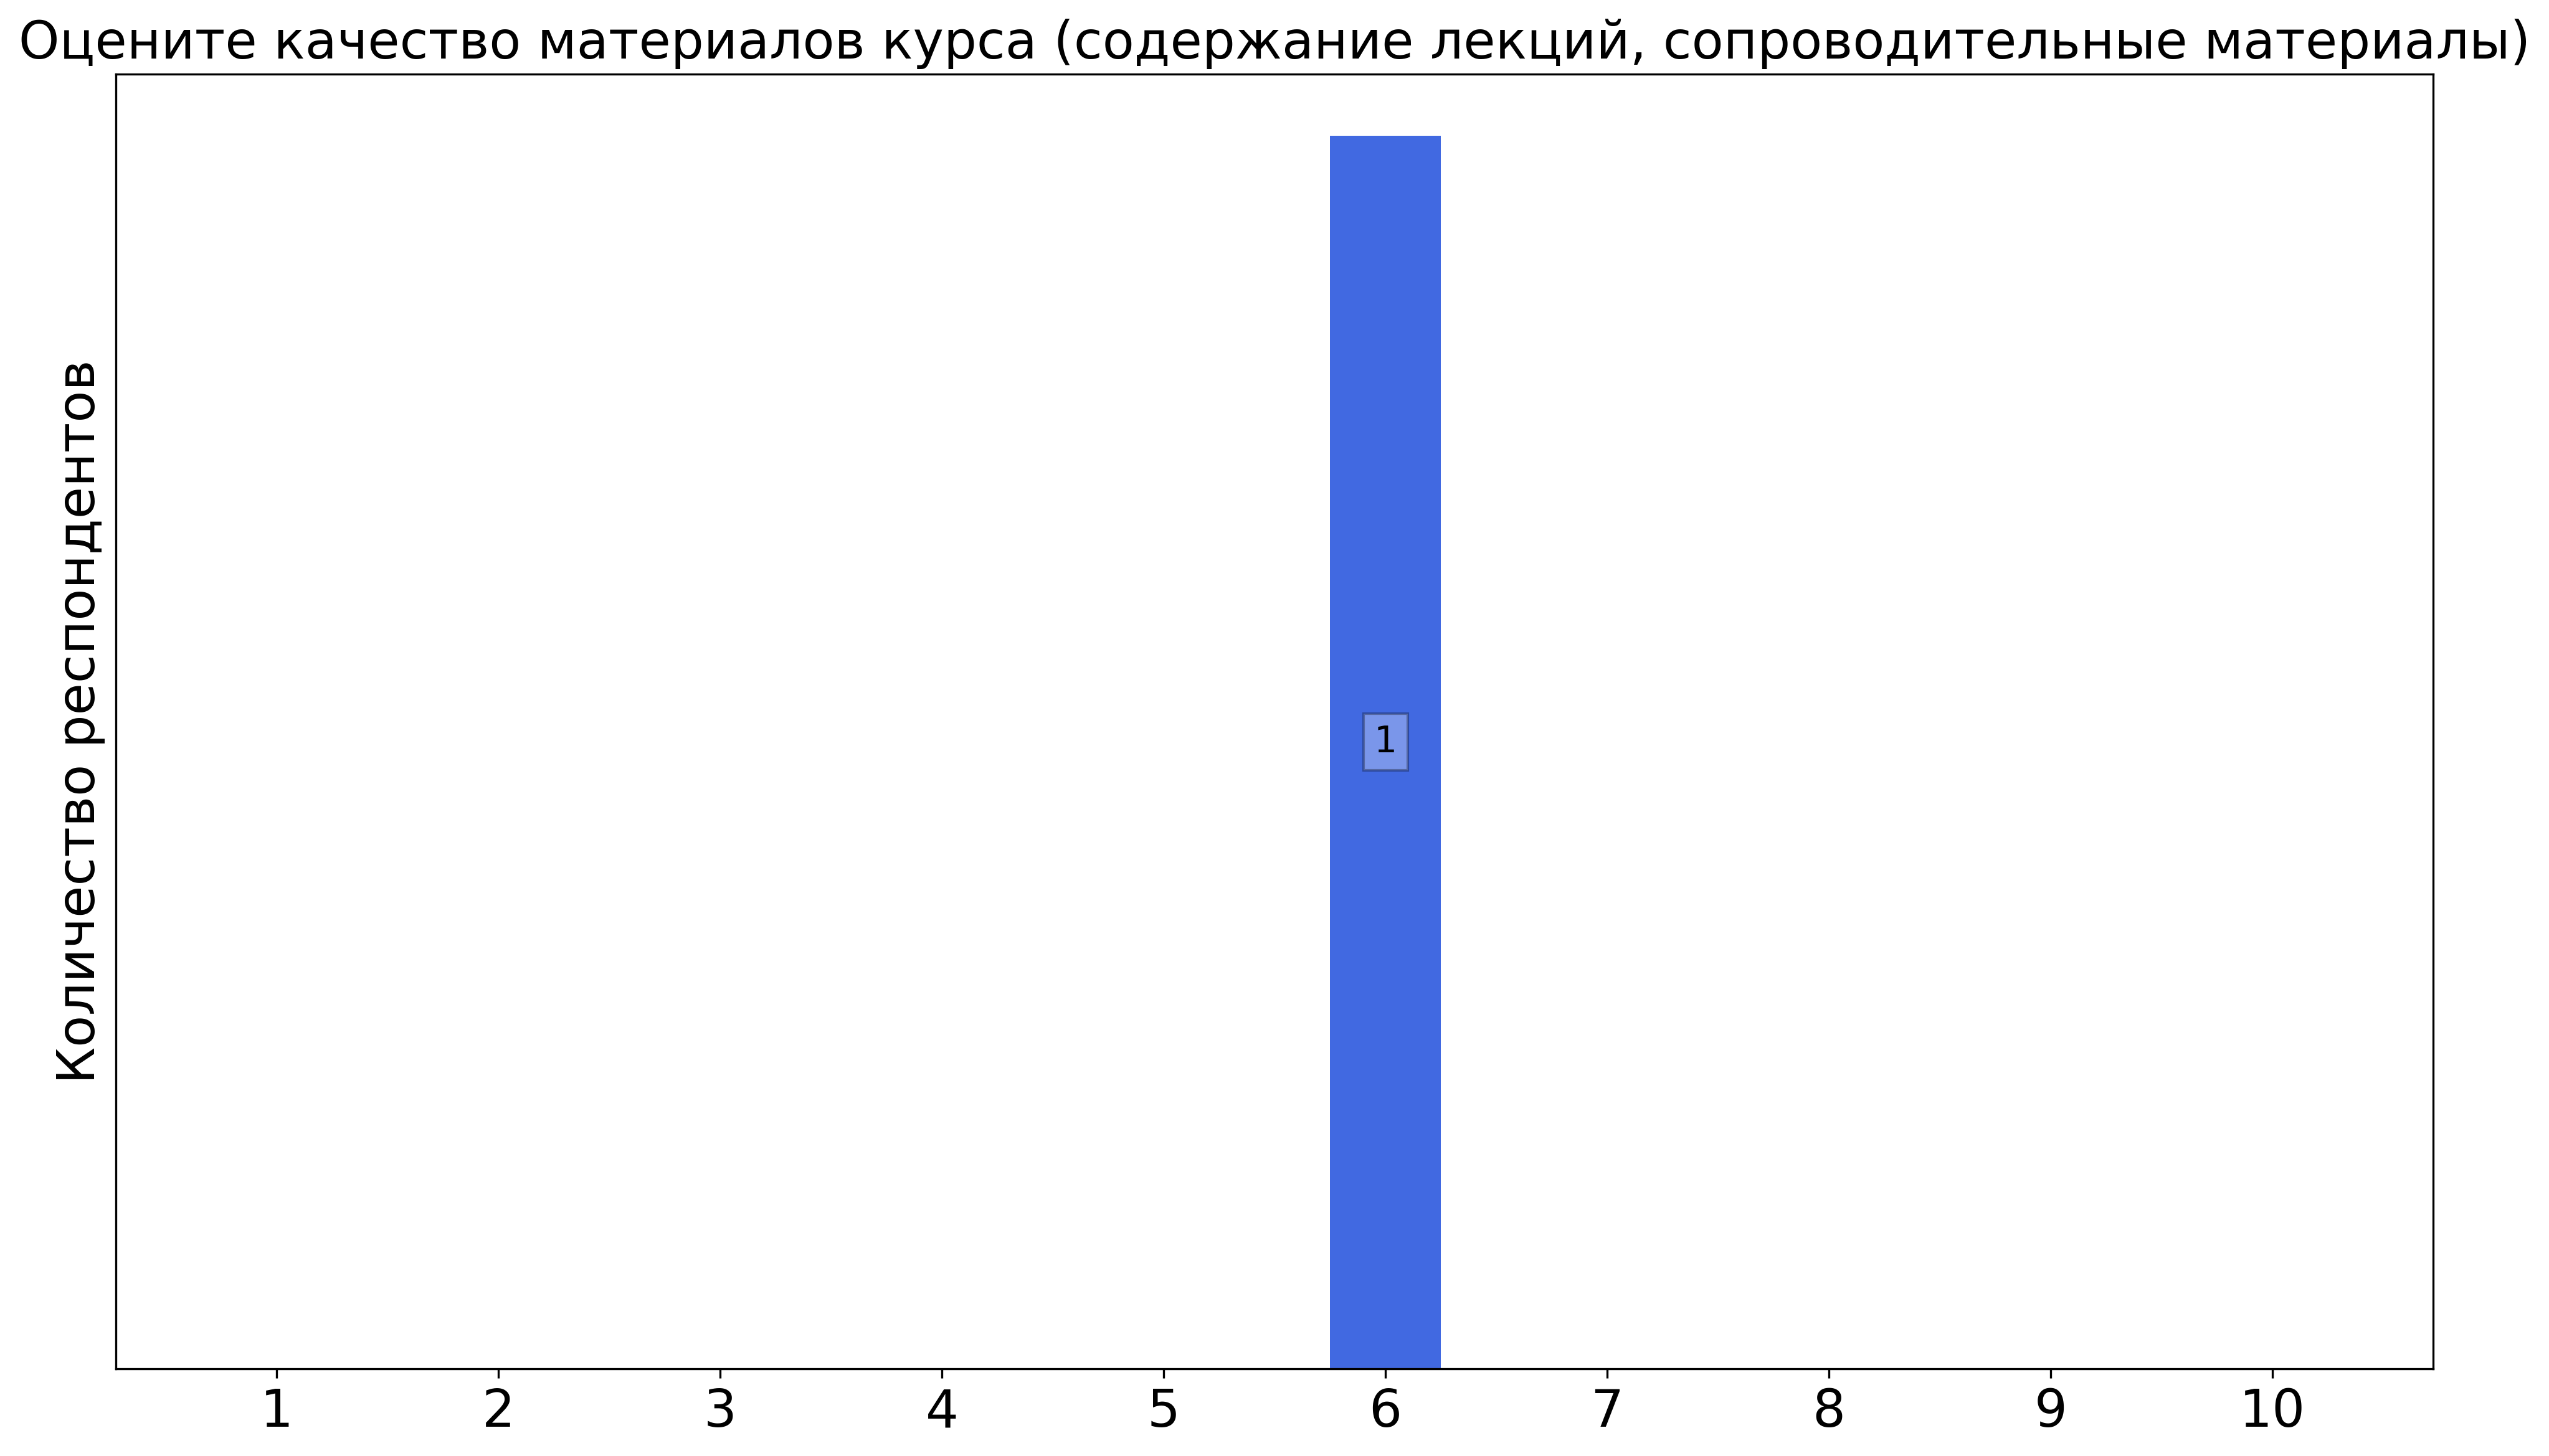
\includegraphics[width=\textwidth]{images/3 course/ТФКП/lecturer-marks-Половинкин Е.С.-1.png}
            \end{subfigure}
            \begin{subfigure}[b]{0.45\textwidth}
                \centering
                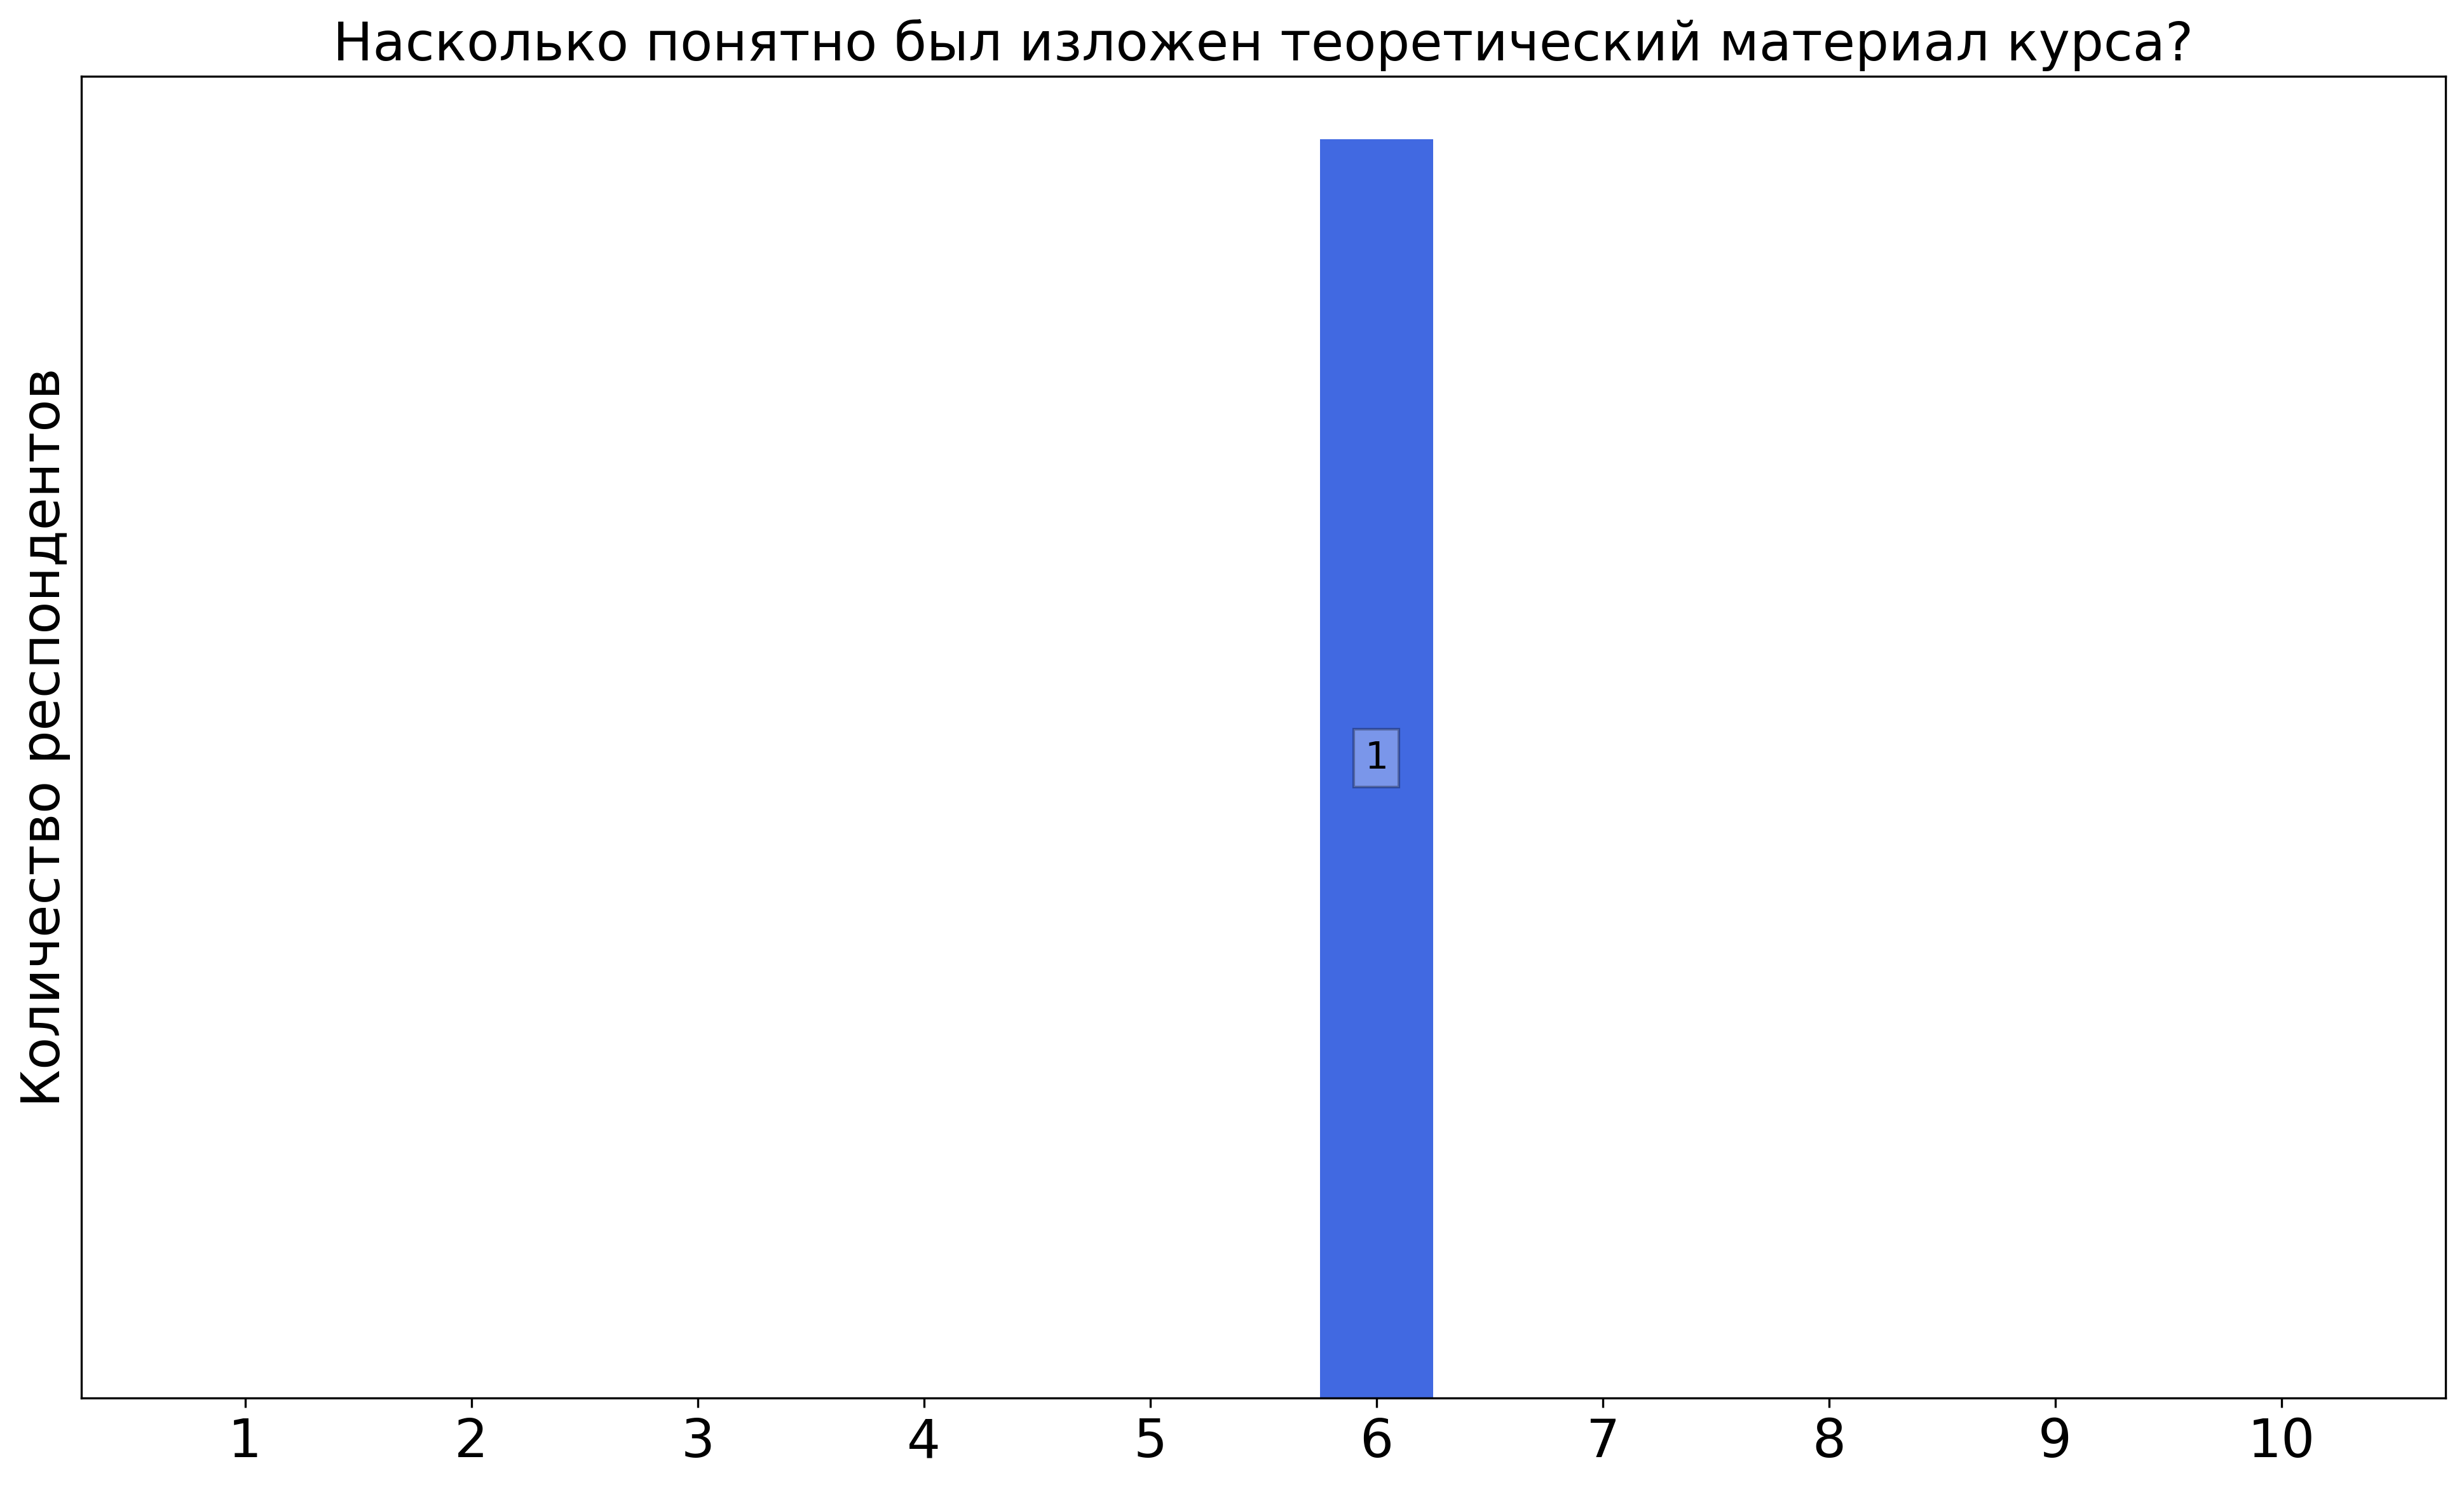
\includegraphics[width=\textwidth]{images/3 course/ТФКП/lecturer-marks-Половинкин Е.С.-2.png}
            \end{subfigure}
            \begin{subfigure}[b]{0.45\textwidth}
                \centering
                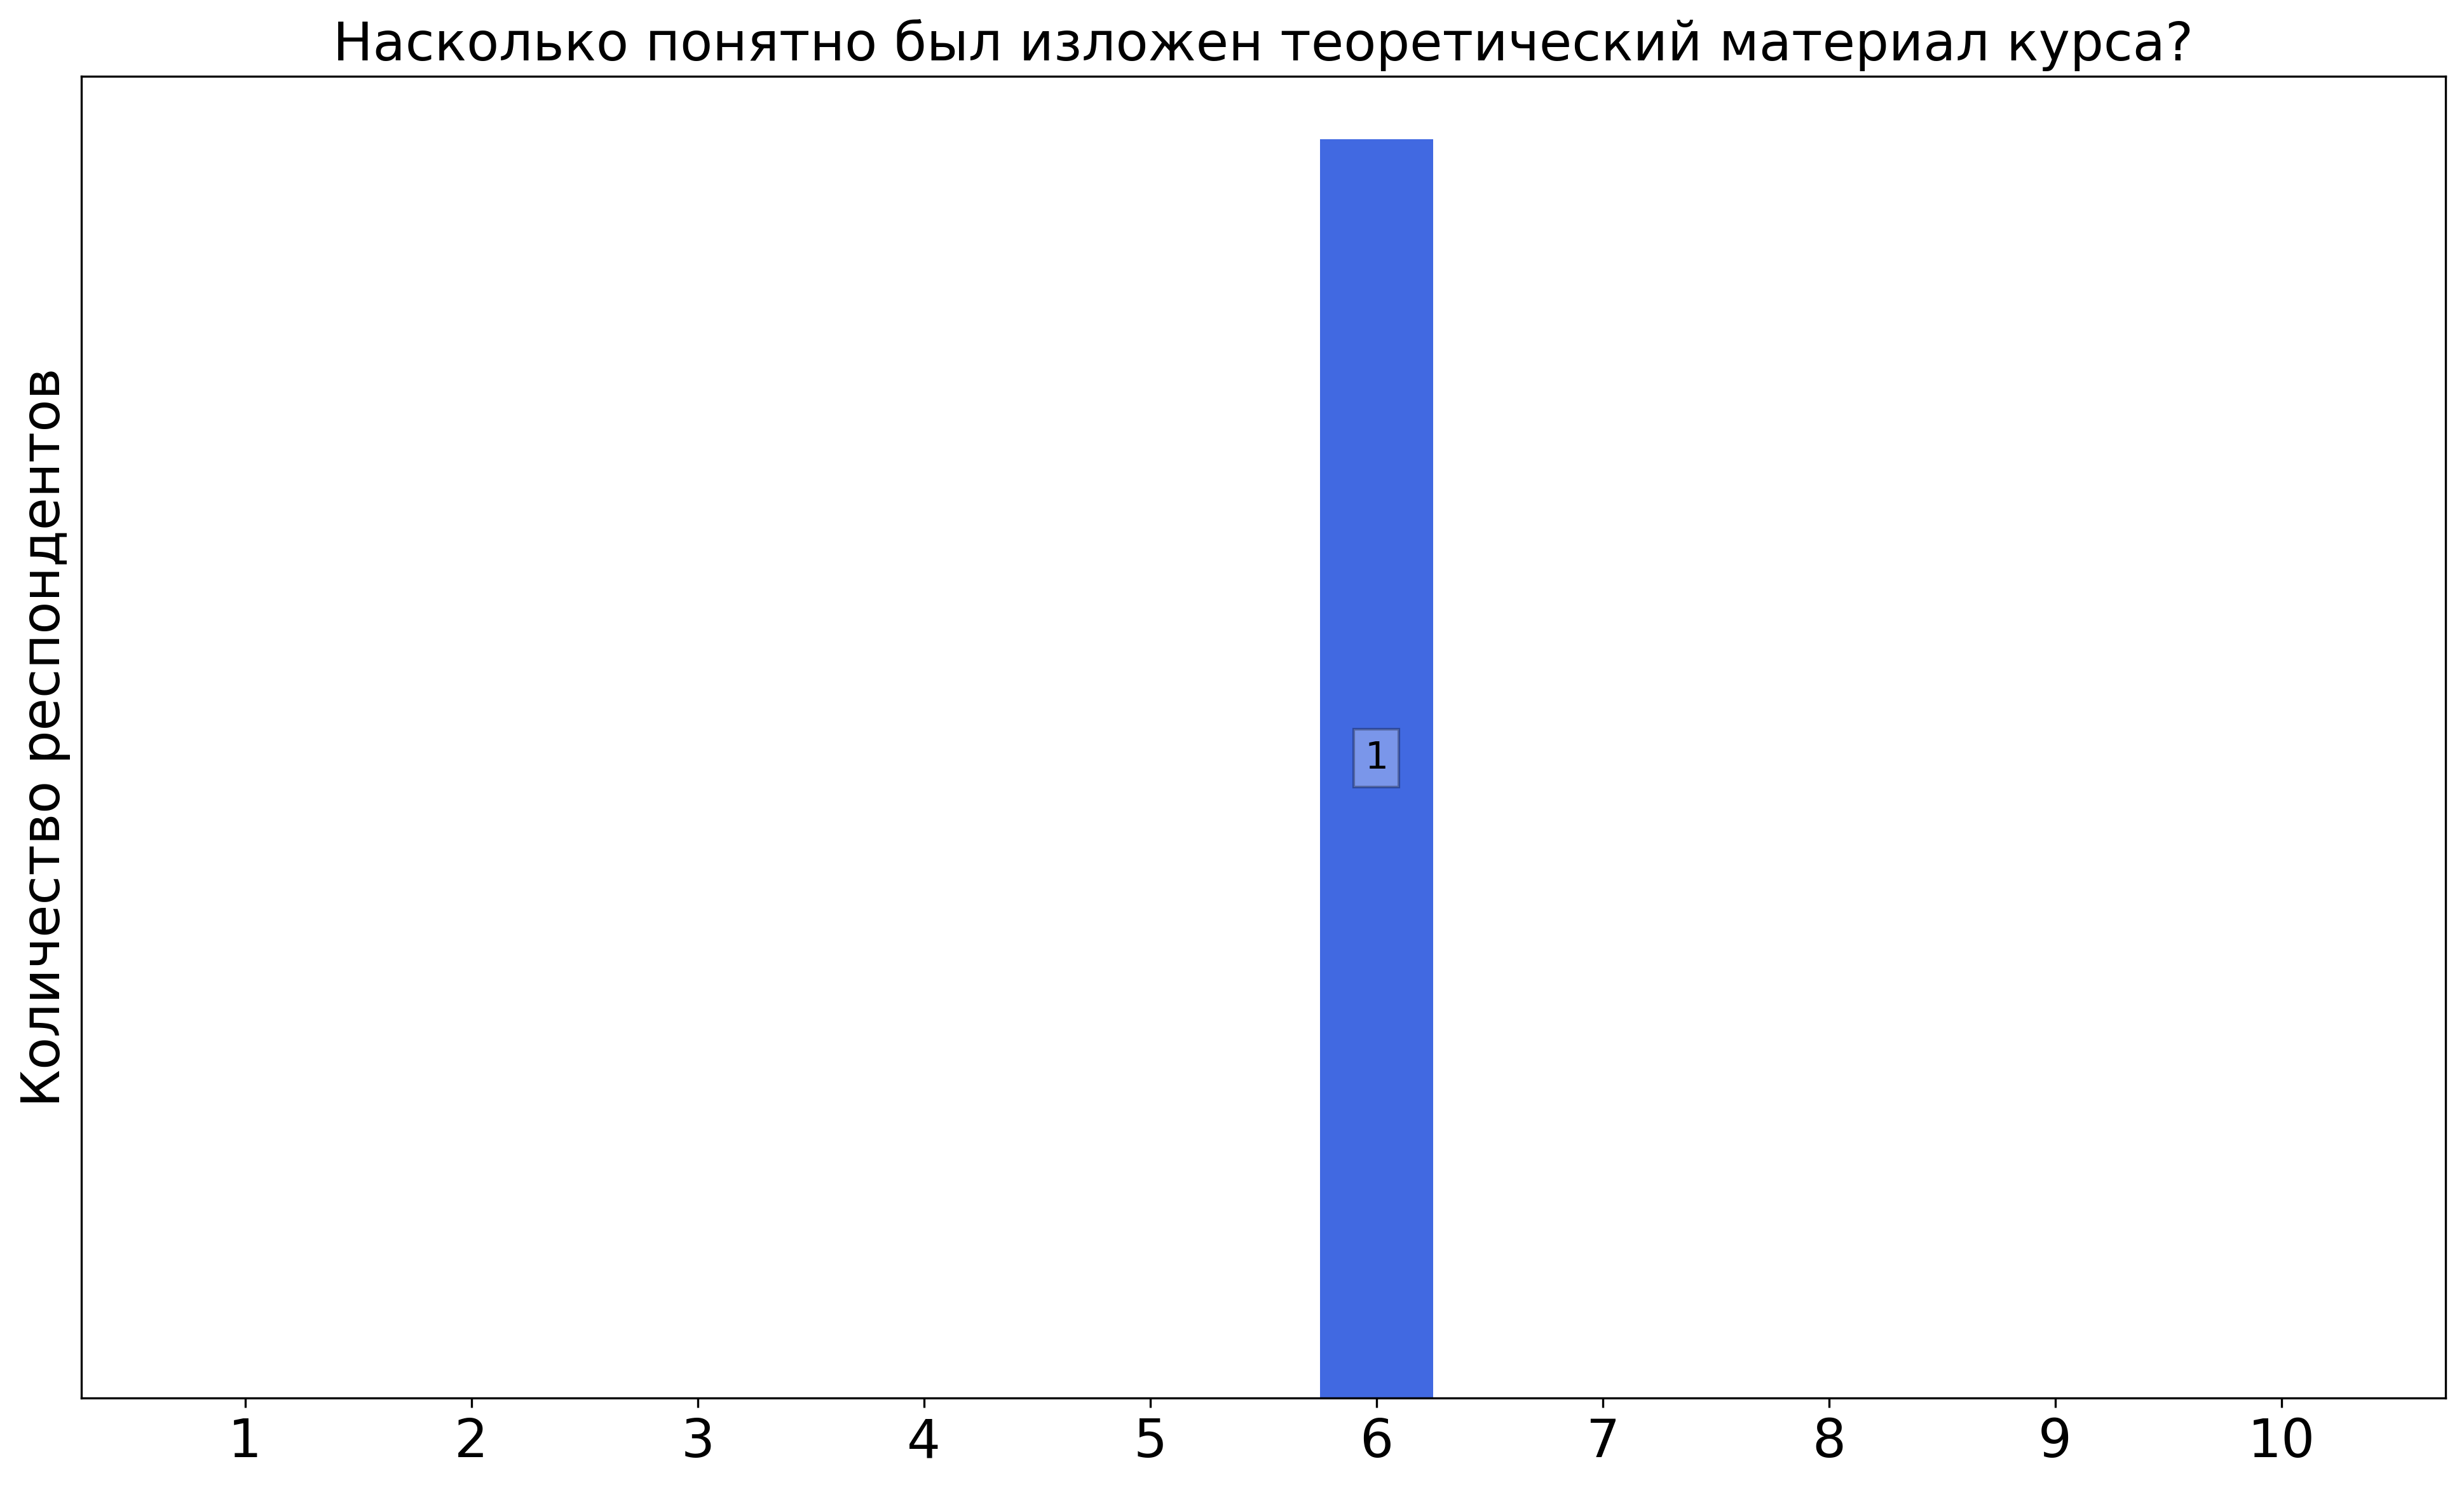
\includegraphics[width=\textwidth]{images/3 course/ТФКП/lecturer-marks-Половинкин Е.С.-2.png}
            \end{subfigure}	
            \begin{subfigure}[b]{0.45\textwidth}
                \centering
                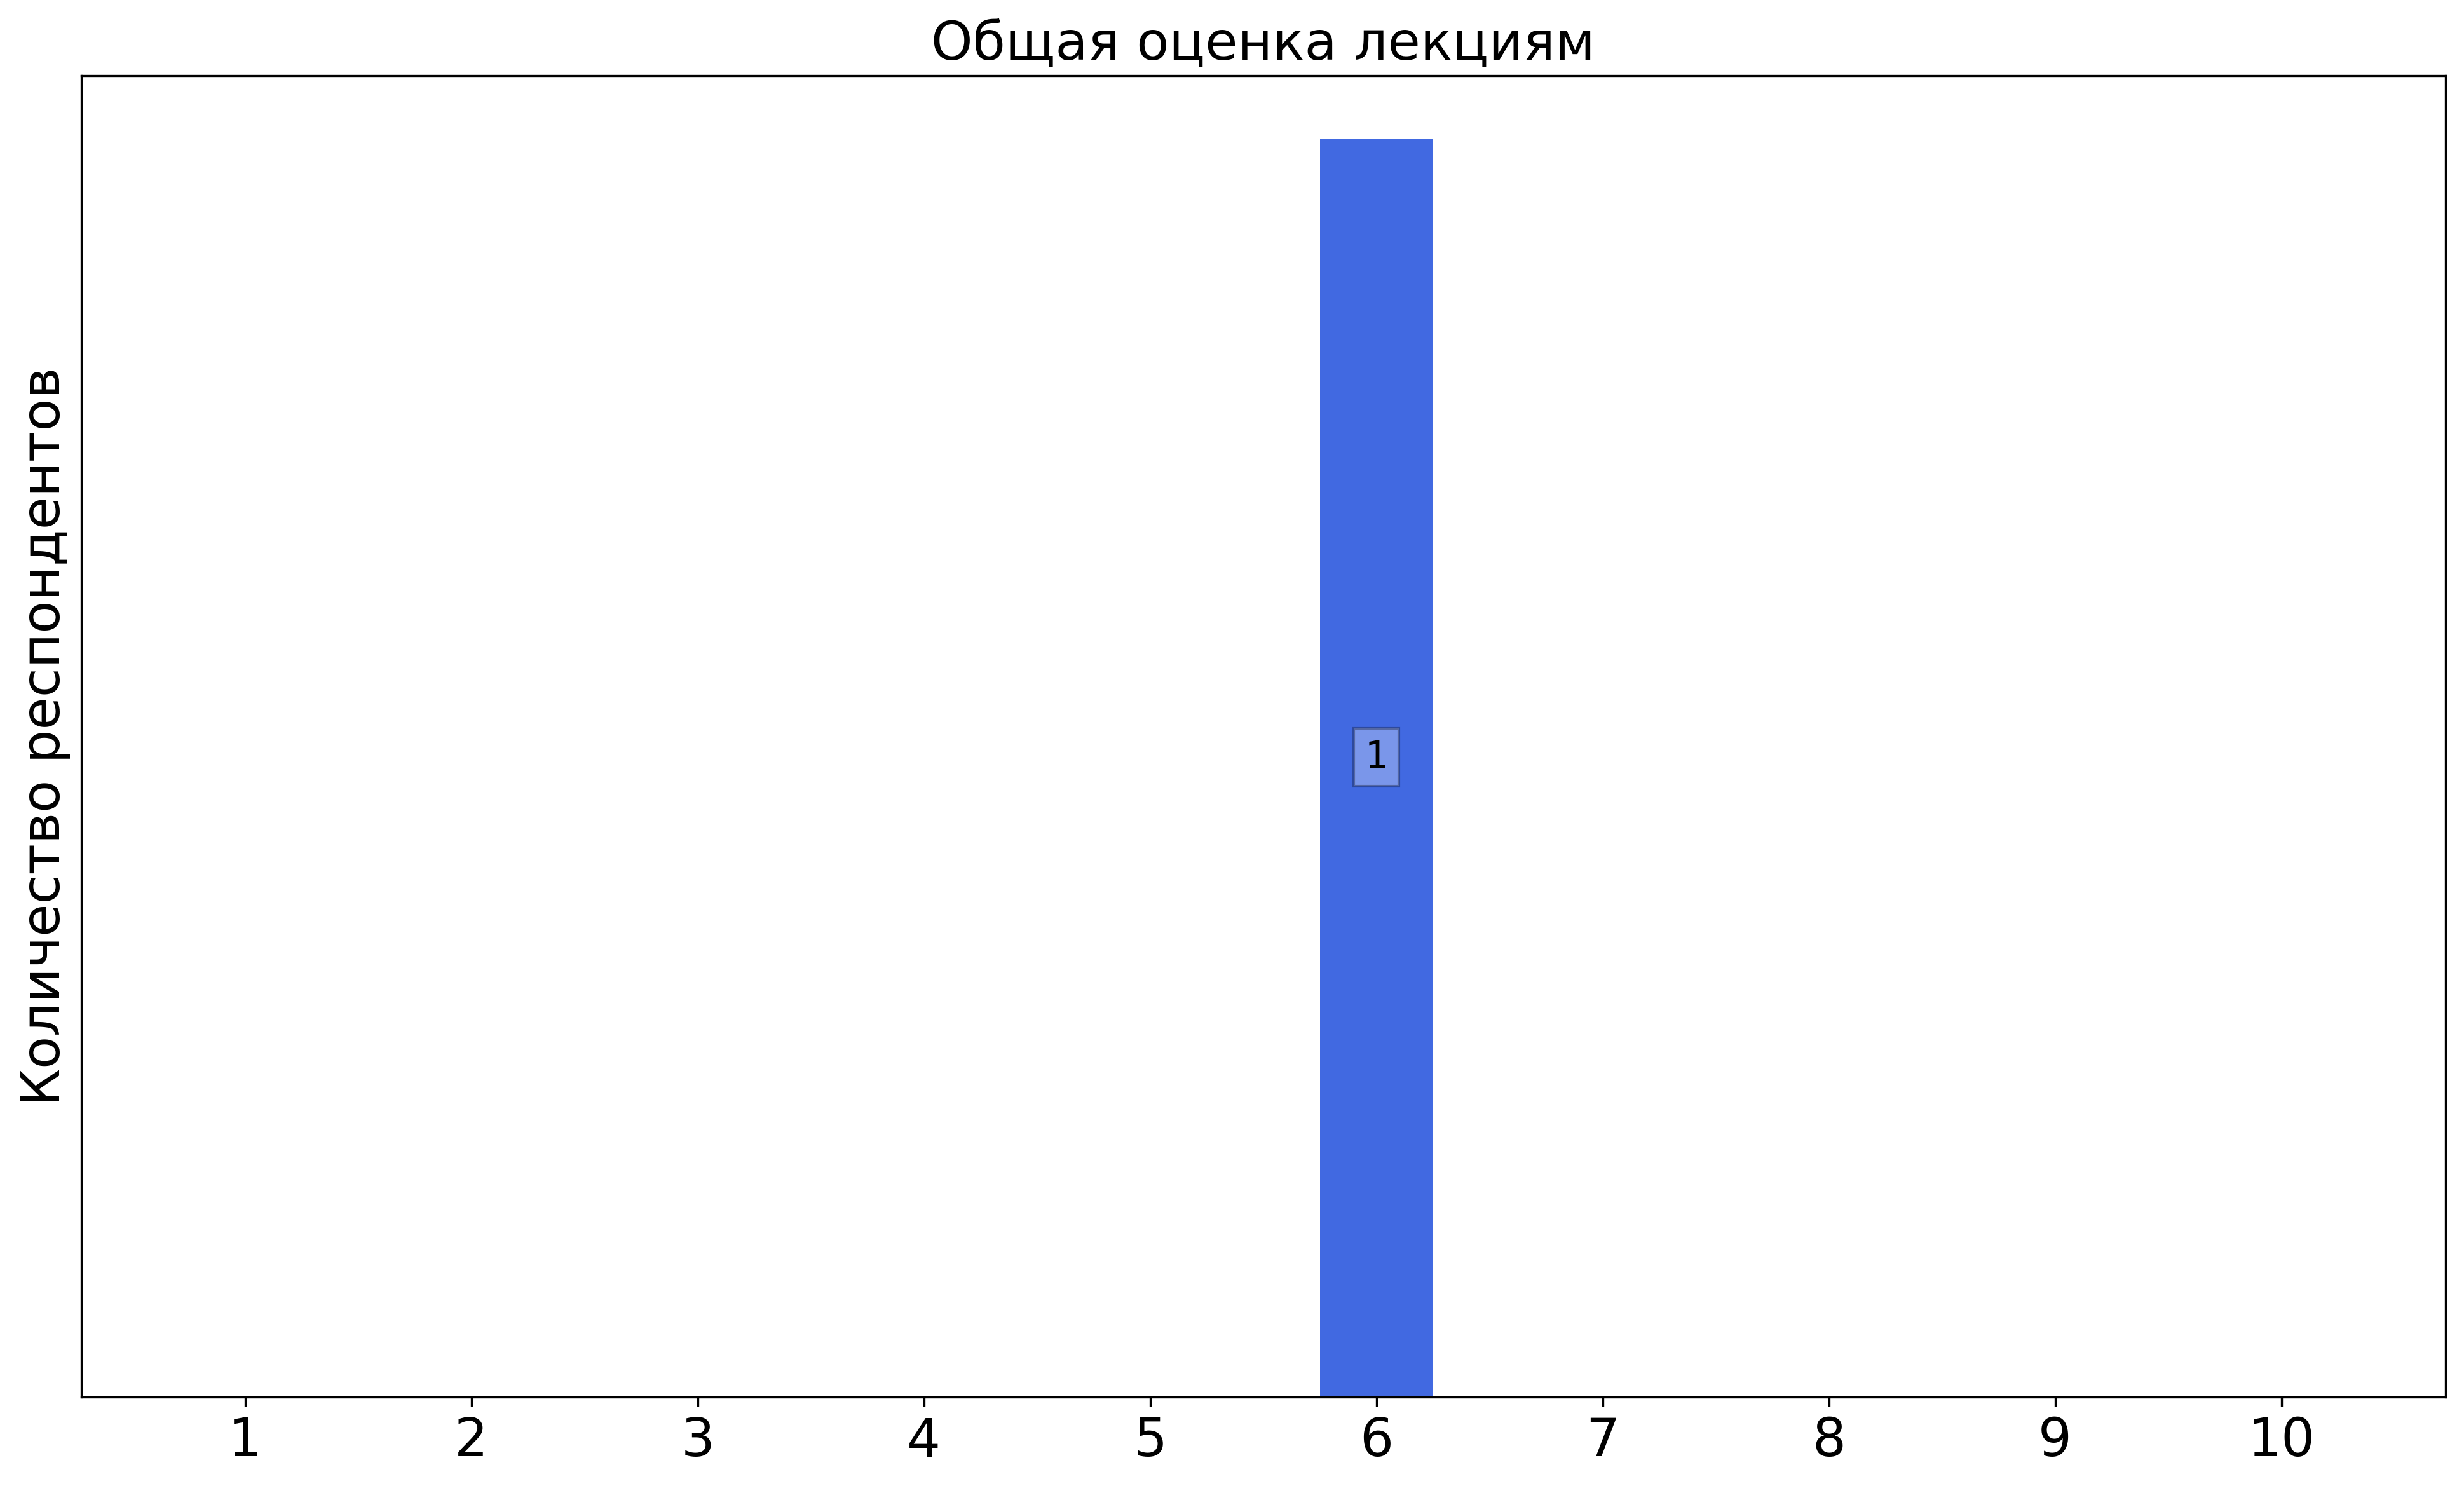
\includegraphics[width=\textwidth]{images/3 course/ТФКП/lecturer-marks-Половинкин Е.С.-3.png}
            \end{subfigure}
            \caption{Оценки респондентов о качестве преподавания лекций по курсу <<ТФКП>>}
        \end{figure}

        \textbf{Комментарии студентов о лекциях\protect\footnote{сохранены оригинальные орфография и пунктуация}}
            \begin{commentbox} 
                Нельзя , Евгений Сергеевич, экзамен так требовательно принимать. У всех и так стресс 
            \end{commentbox} 

    
    \subsubsection{Отзыв студентов о семинарах. Семинарист: Бунаков А.Э.}
		\begin{figure}[H]
			\centering
			\begin{subfigure}[b]{0.45\textwidth}
				\centering
				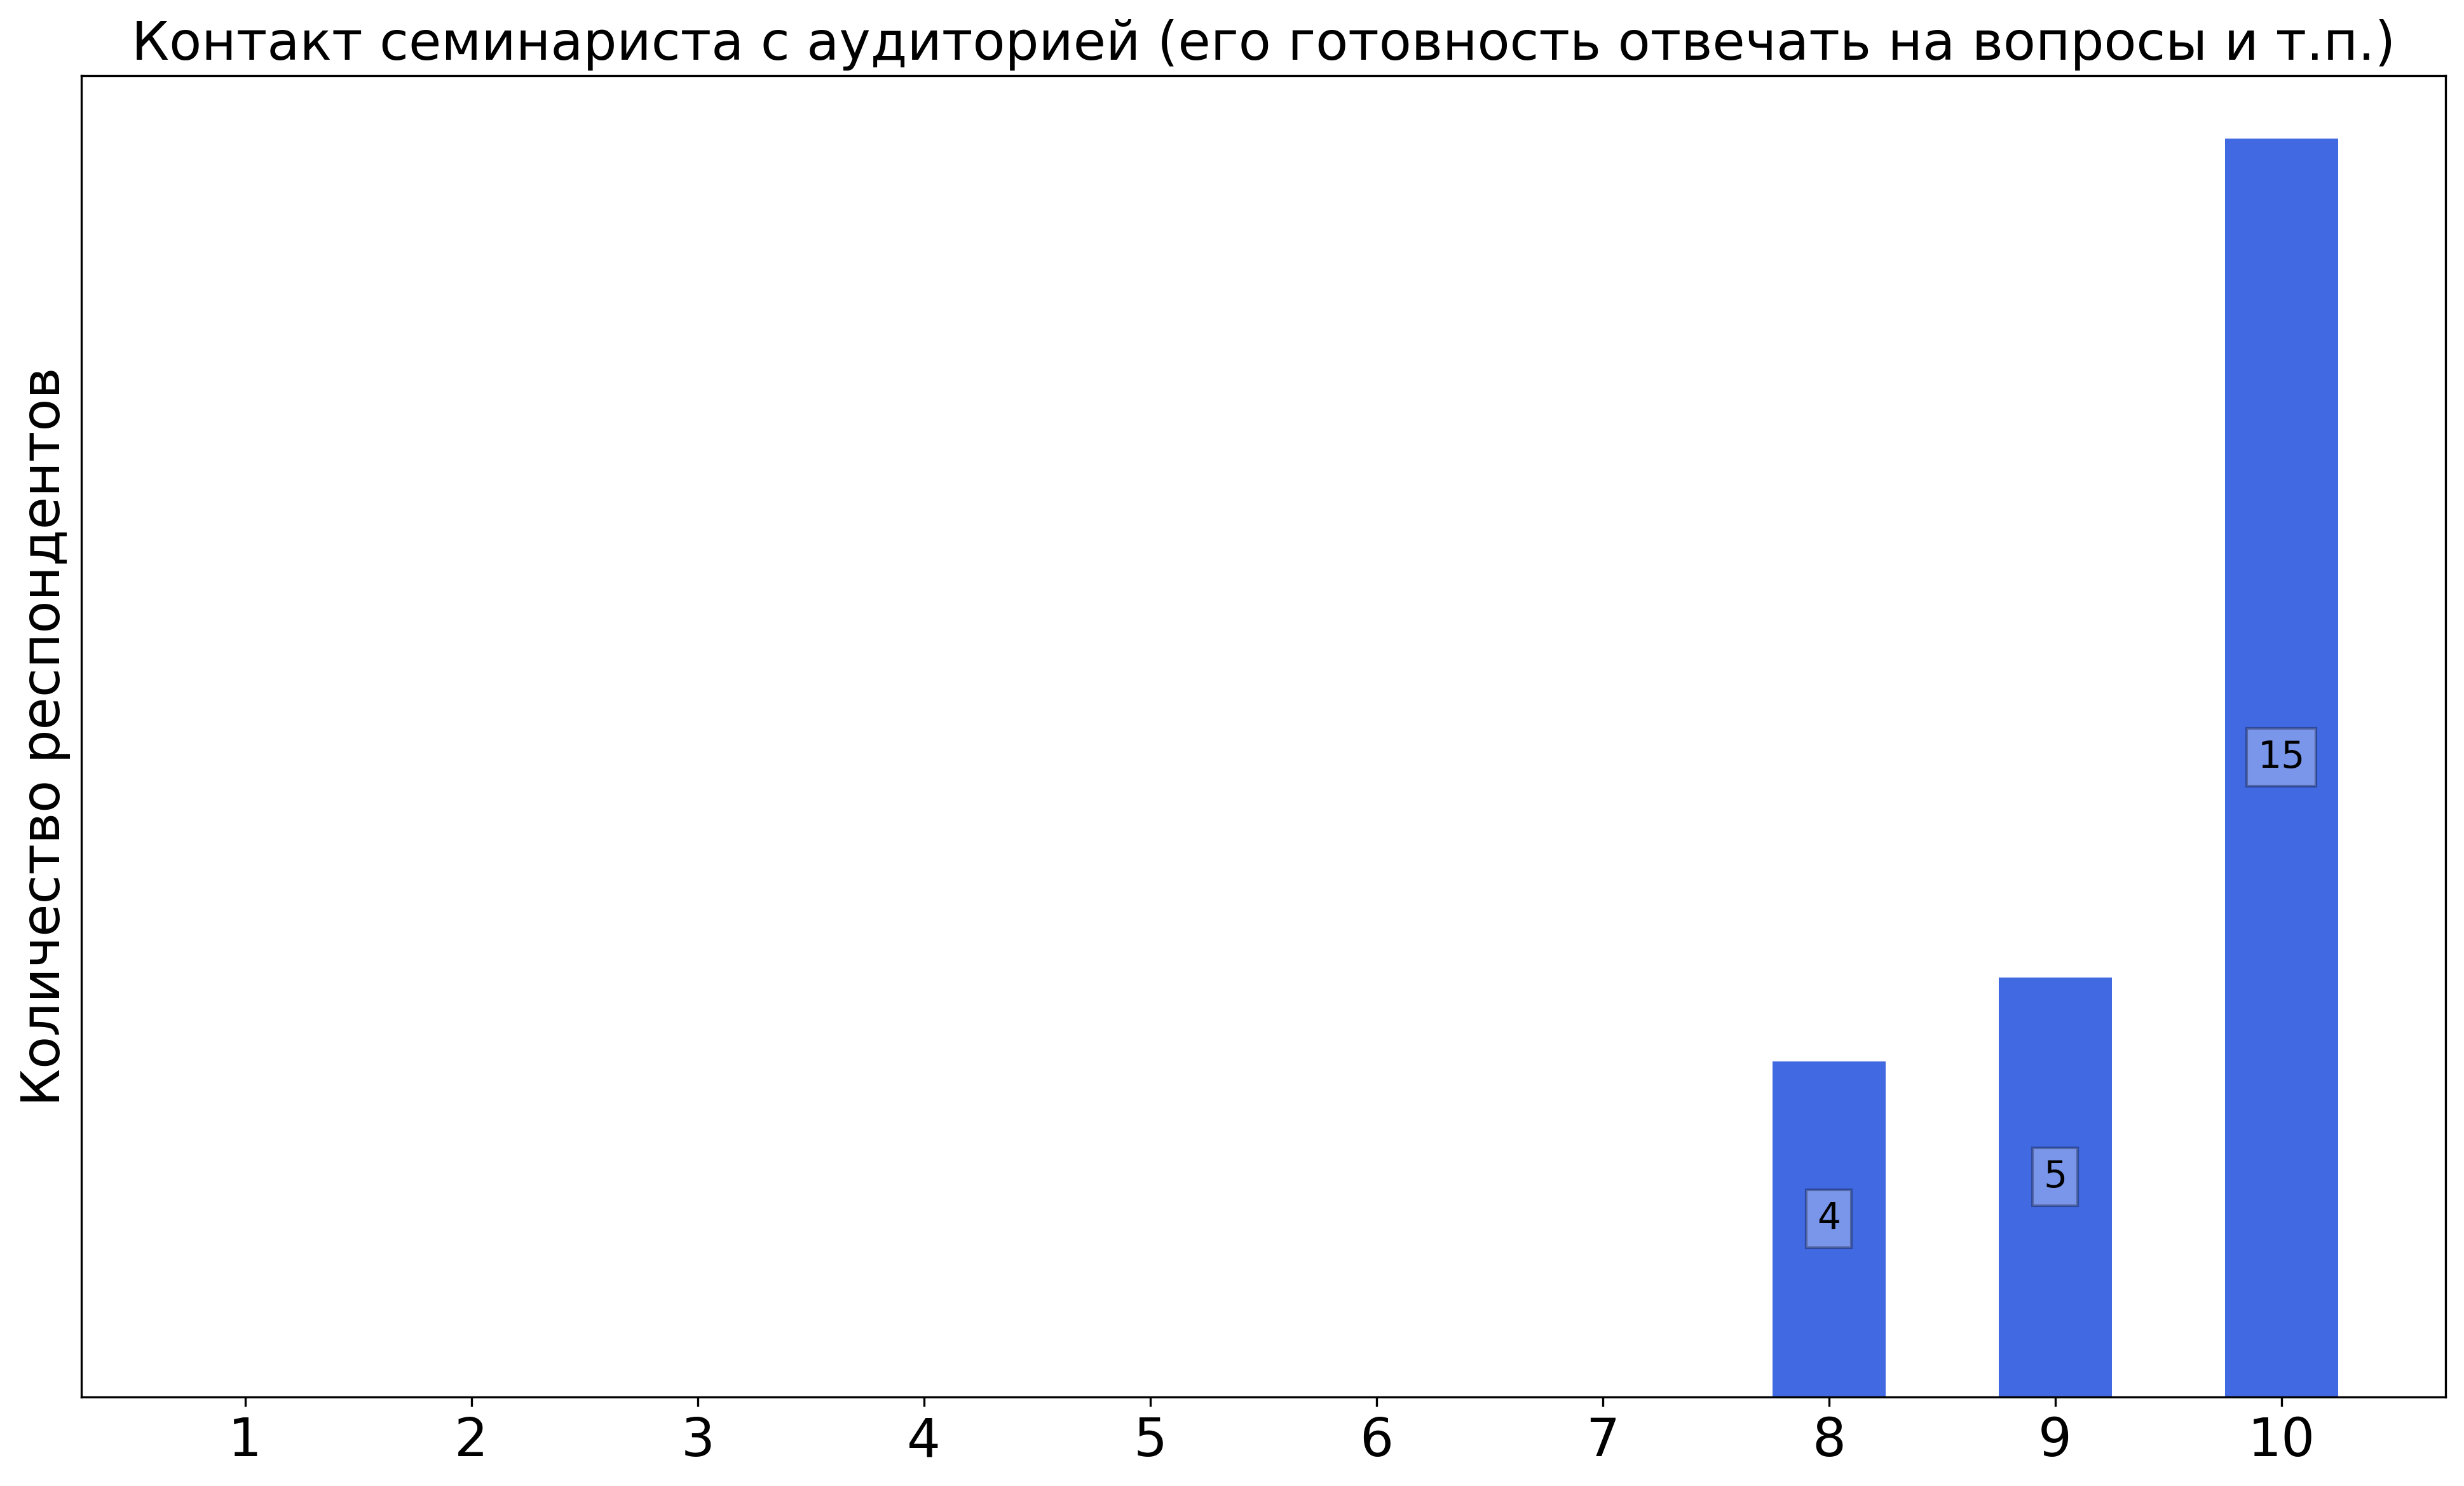
\includegraphics[width=\textwidth]{images/3 course/ТФКП/seminarists-marks-Бунаков А.Э.-0.png}
			\end{subfigure}
			\begin{subfigure}[b]{0.45\textwidth}
				\centering
				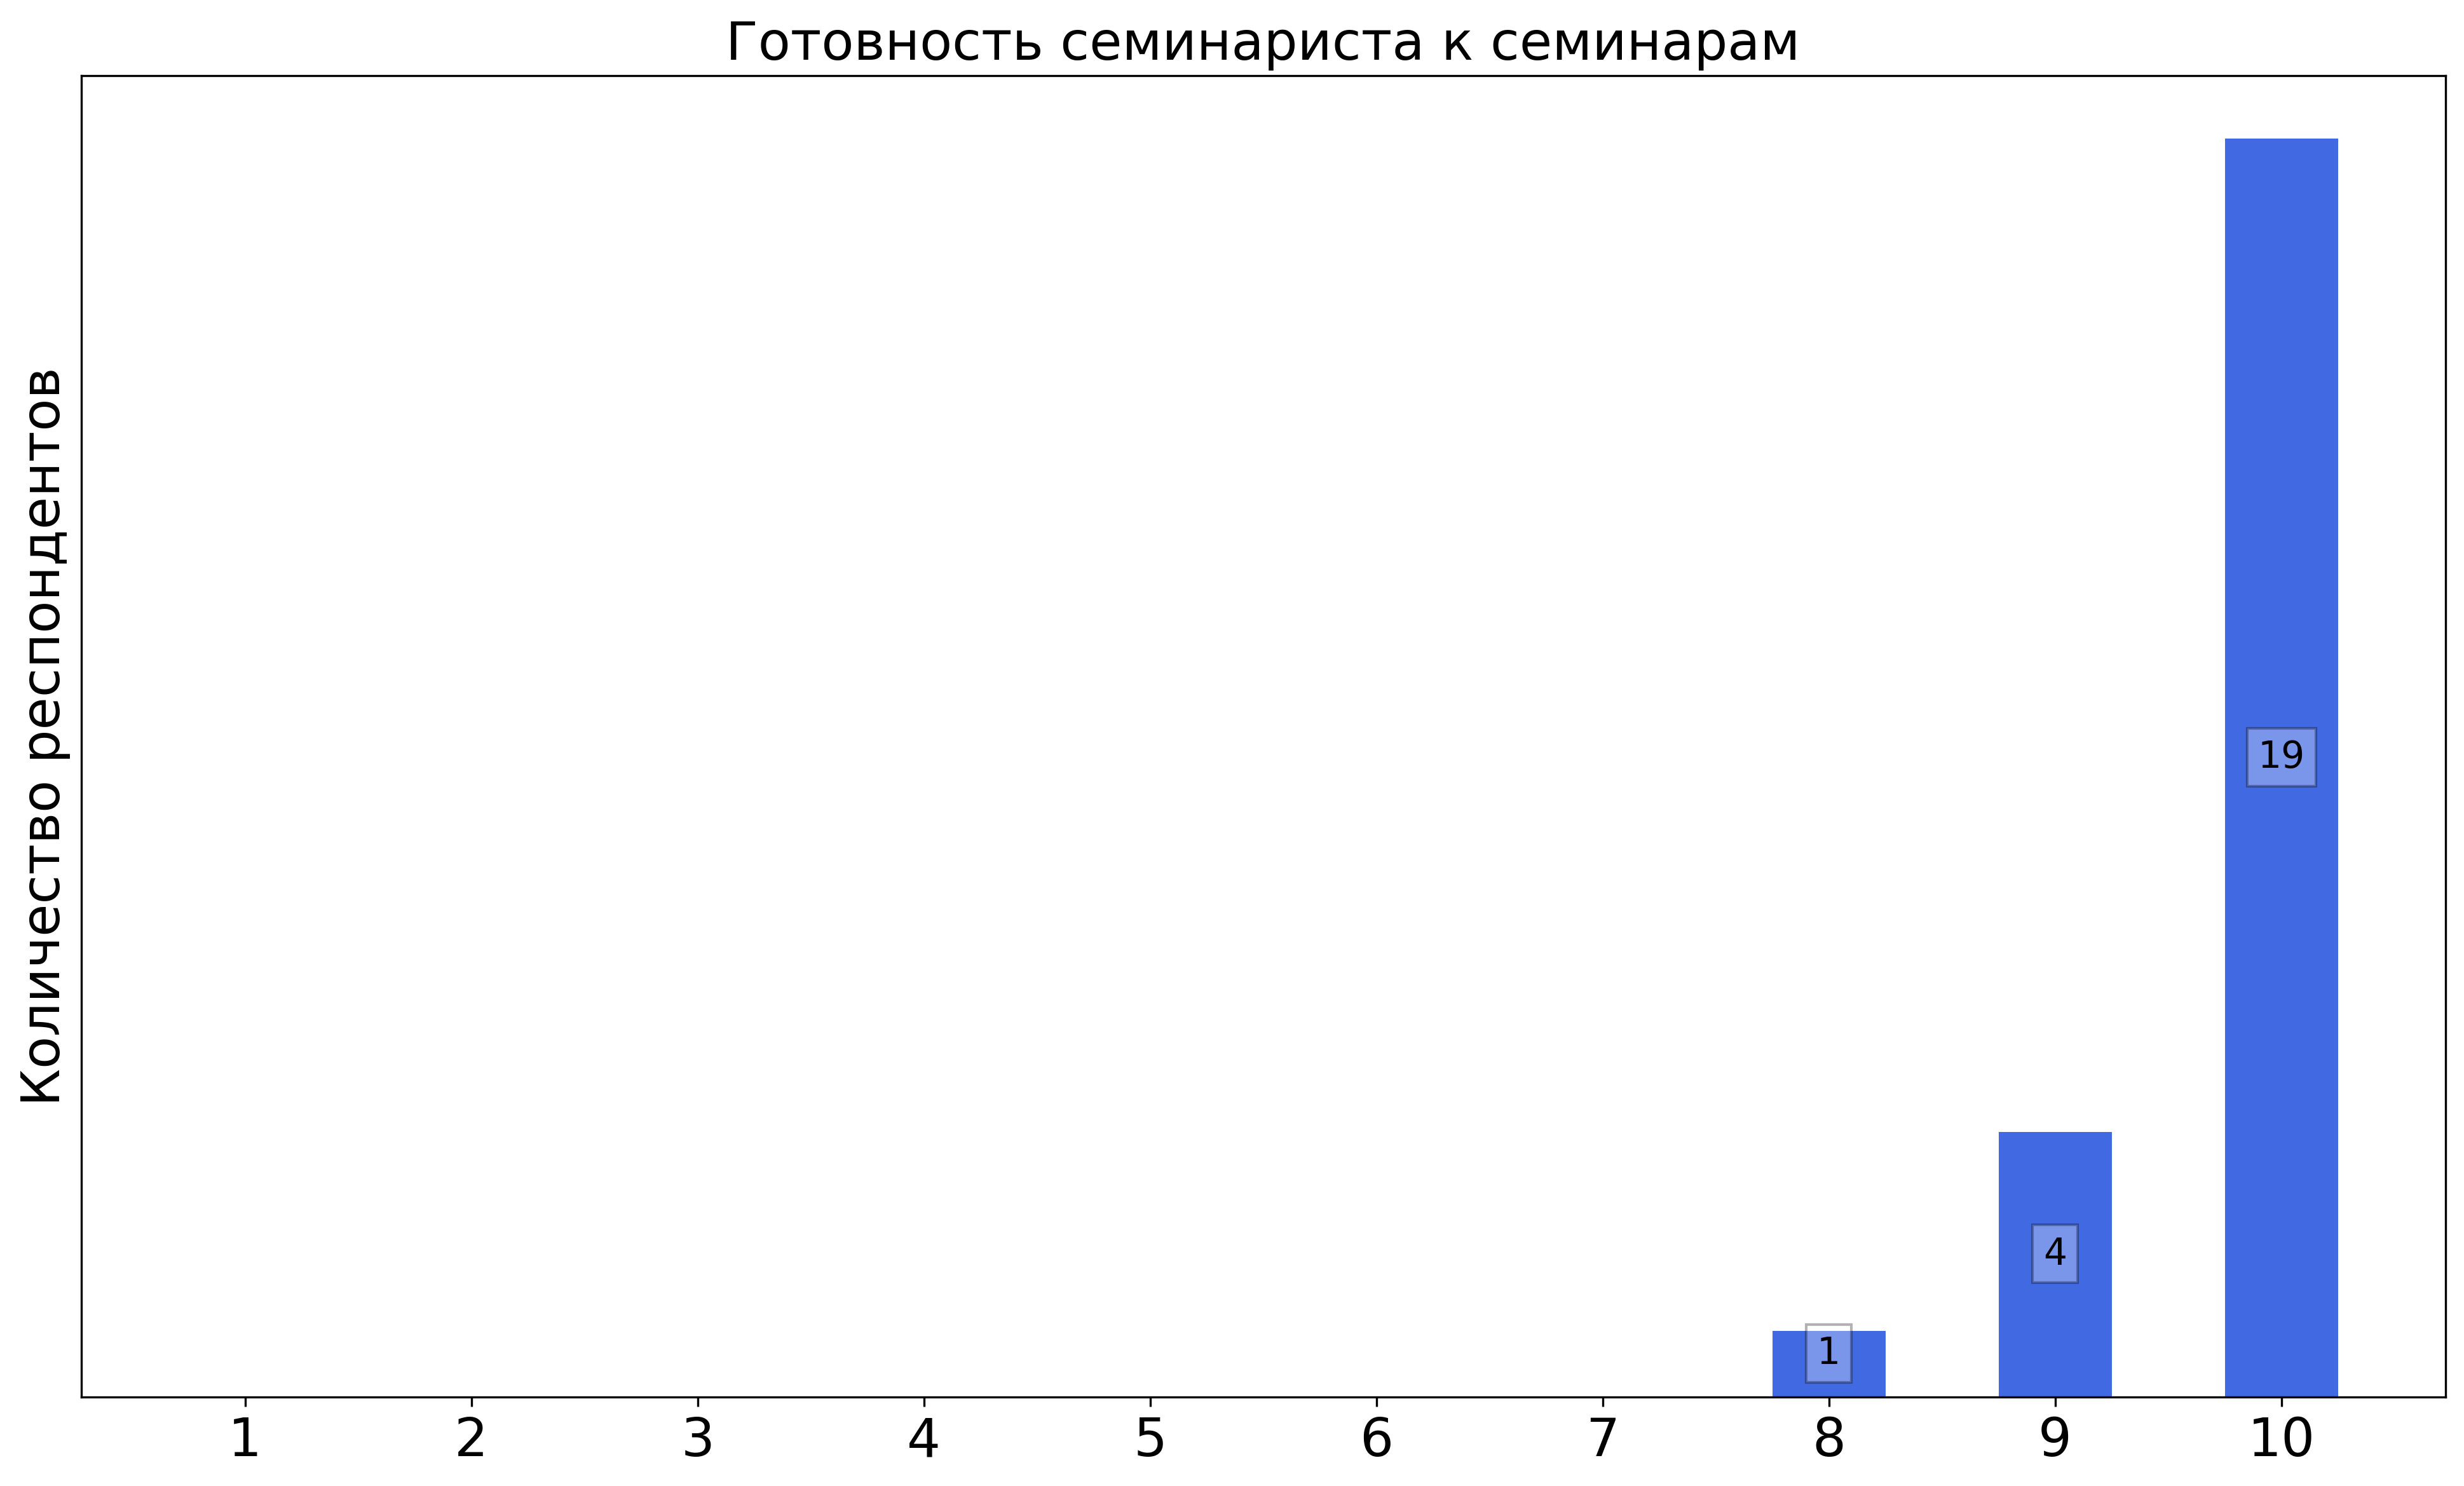
\includegraphics[width=\textwidth]{images/3 course/ТФКП/seminarists-marks-Бунаков А.Э.-1.png}
			\end{subfigure}
			\begin{subfigure}[b]{0.45\textwidth}
				\centering
				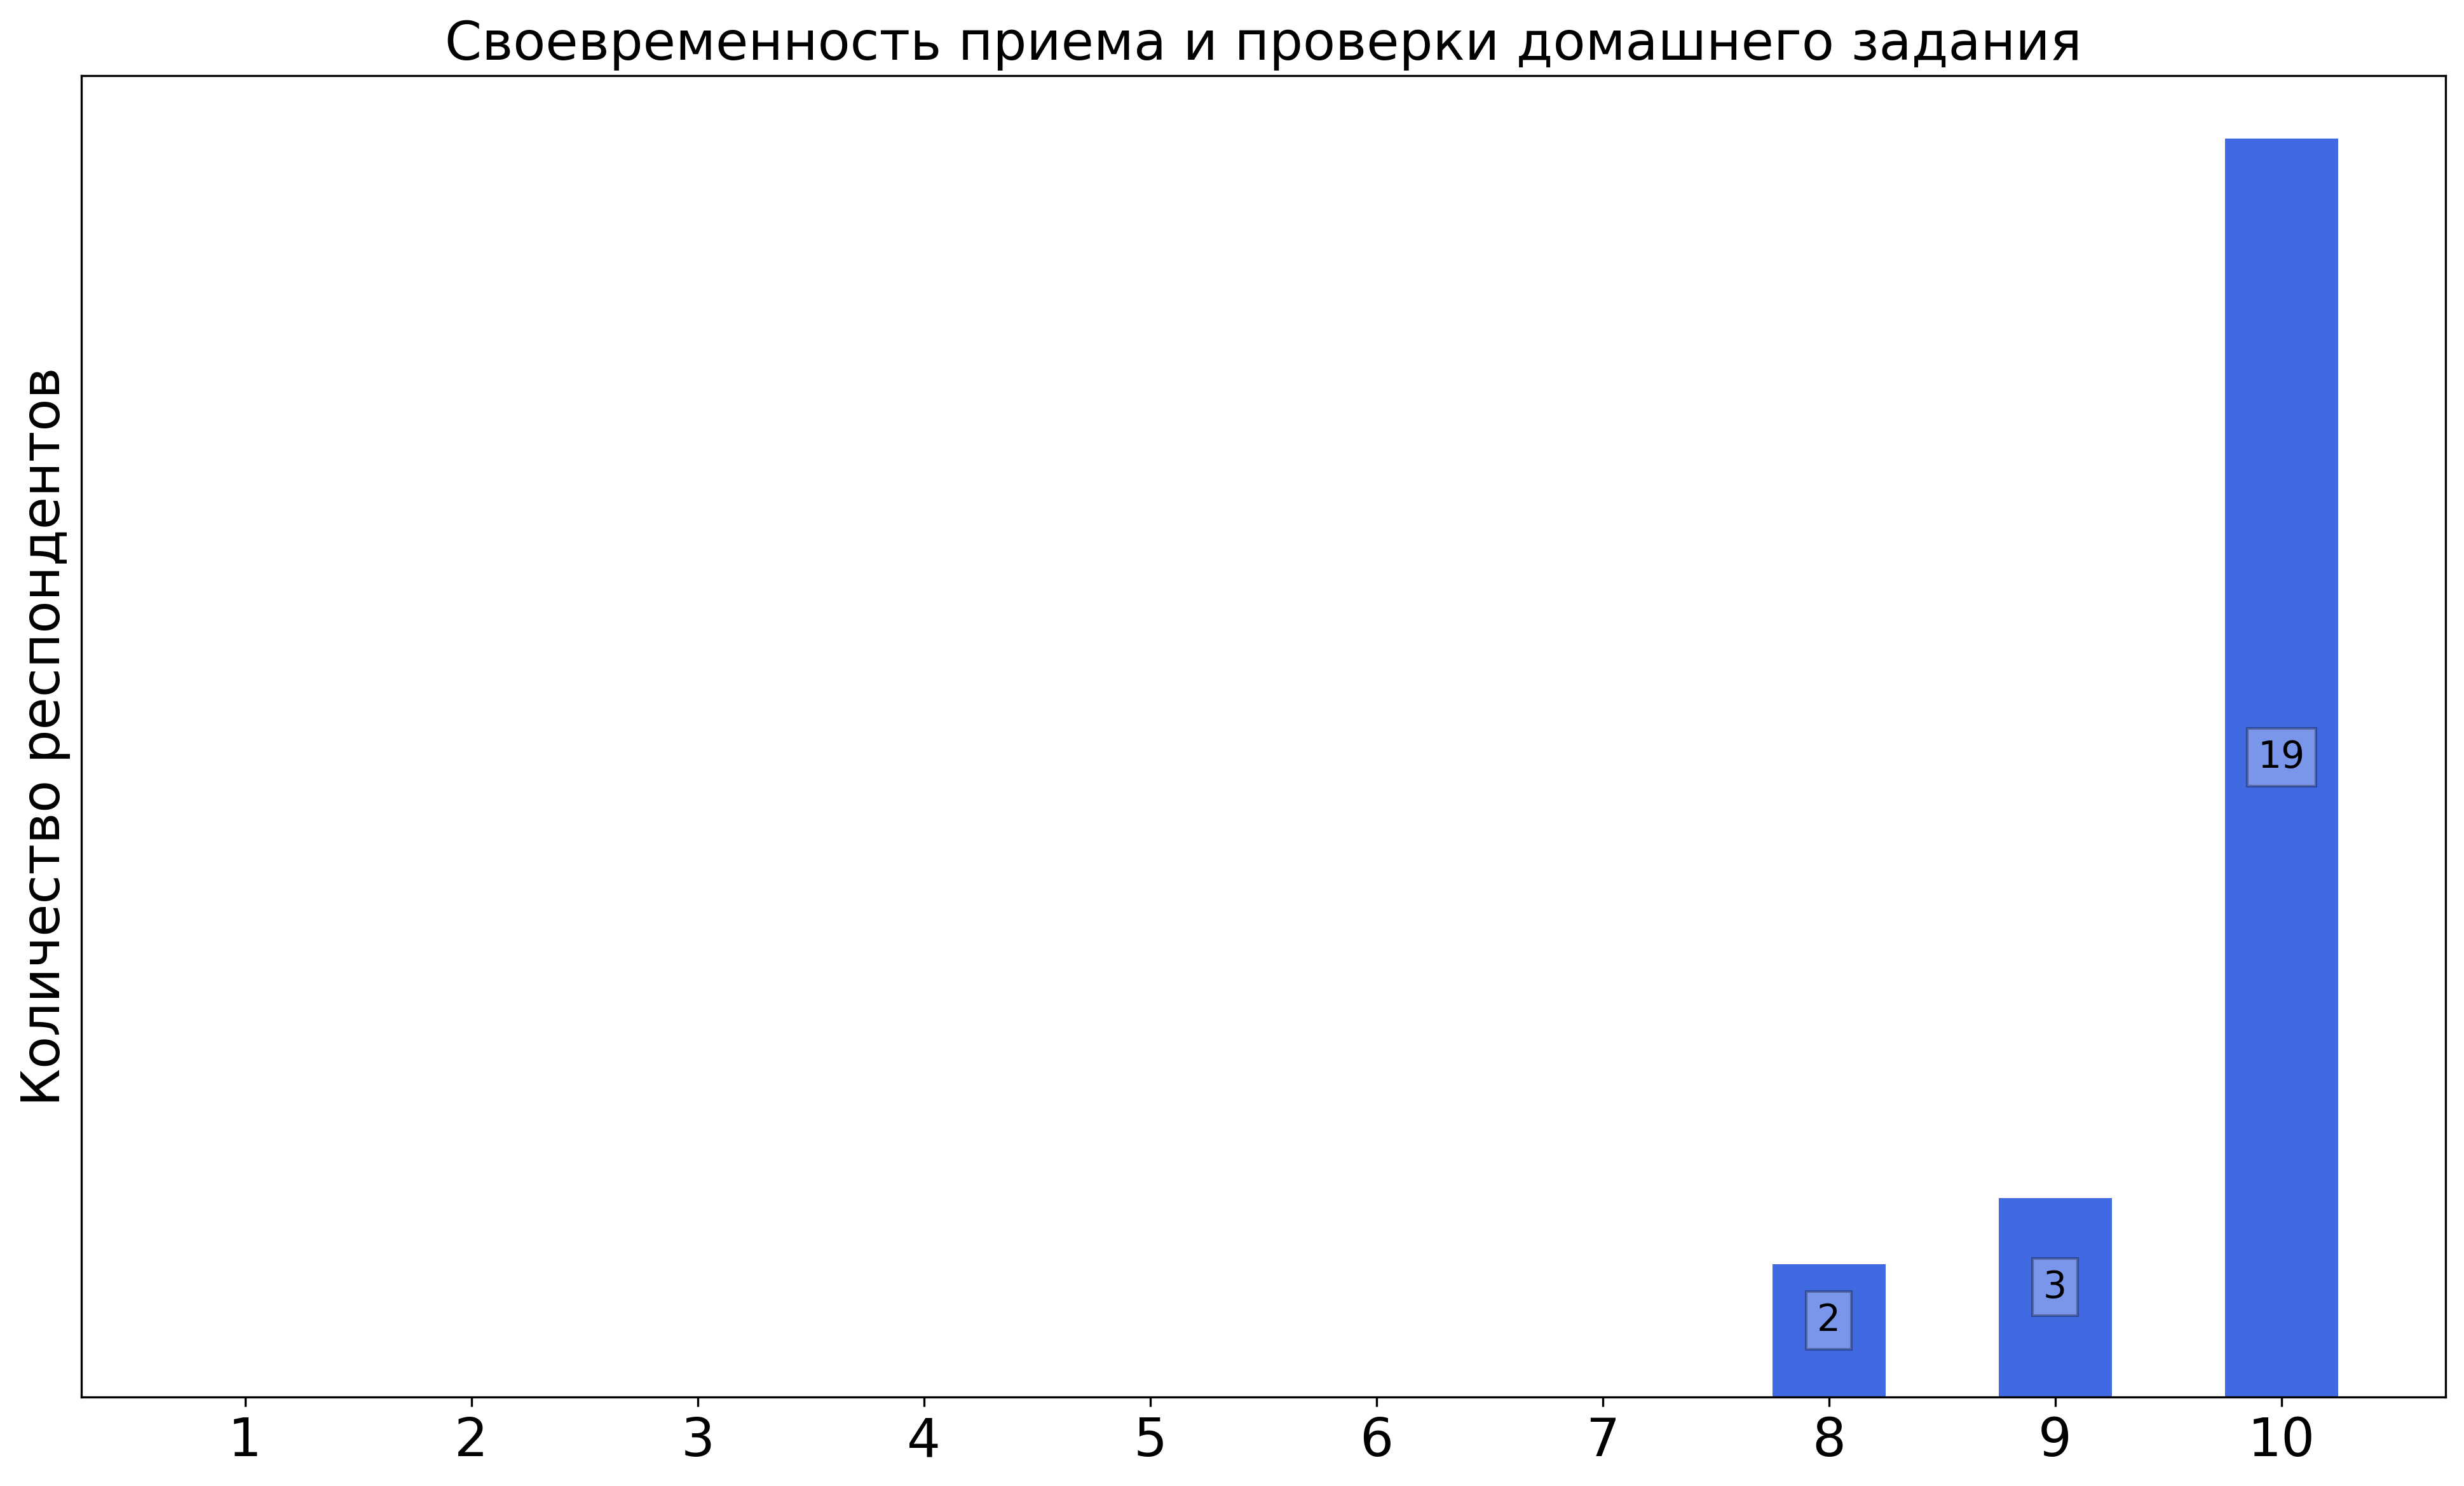
\includegraphics[width=\textwidth]{images/3 course/ТФКП/seminarists-marks-Бунаков А.Э.-2.png}
			\end{subfigure}
			\begin{subfigure}[b]{0.45\textwidth}
				\centering
				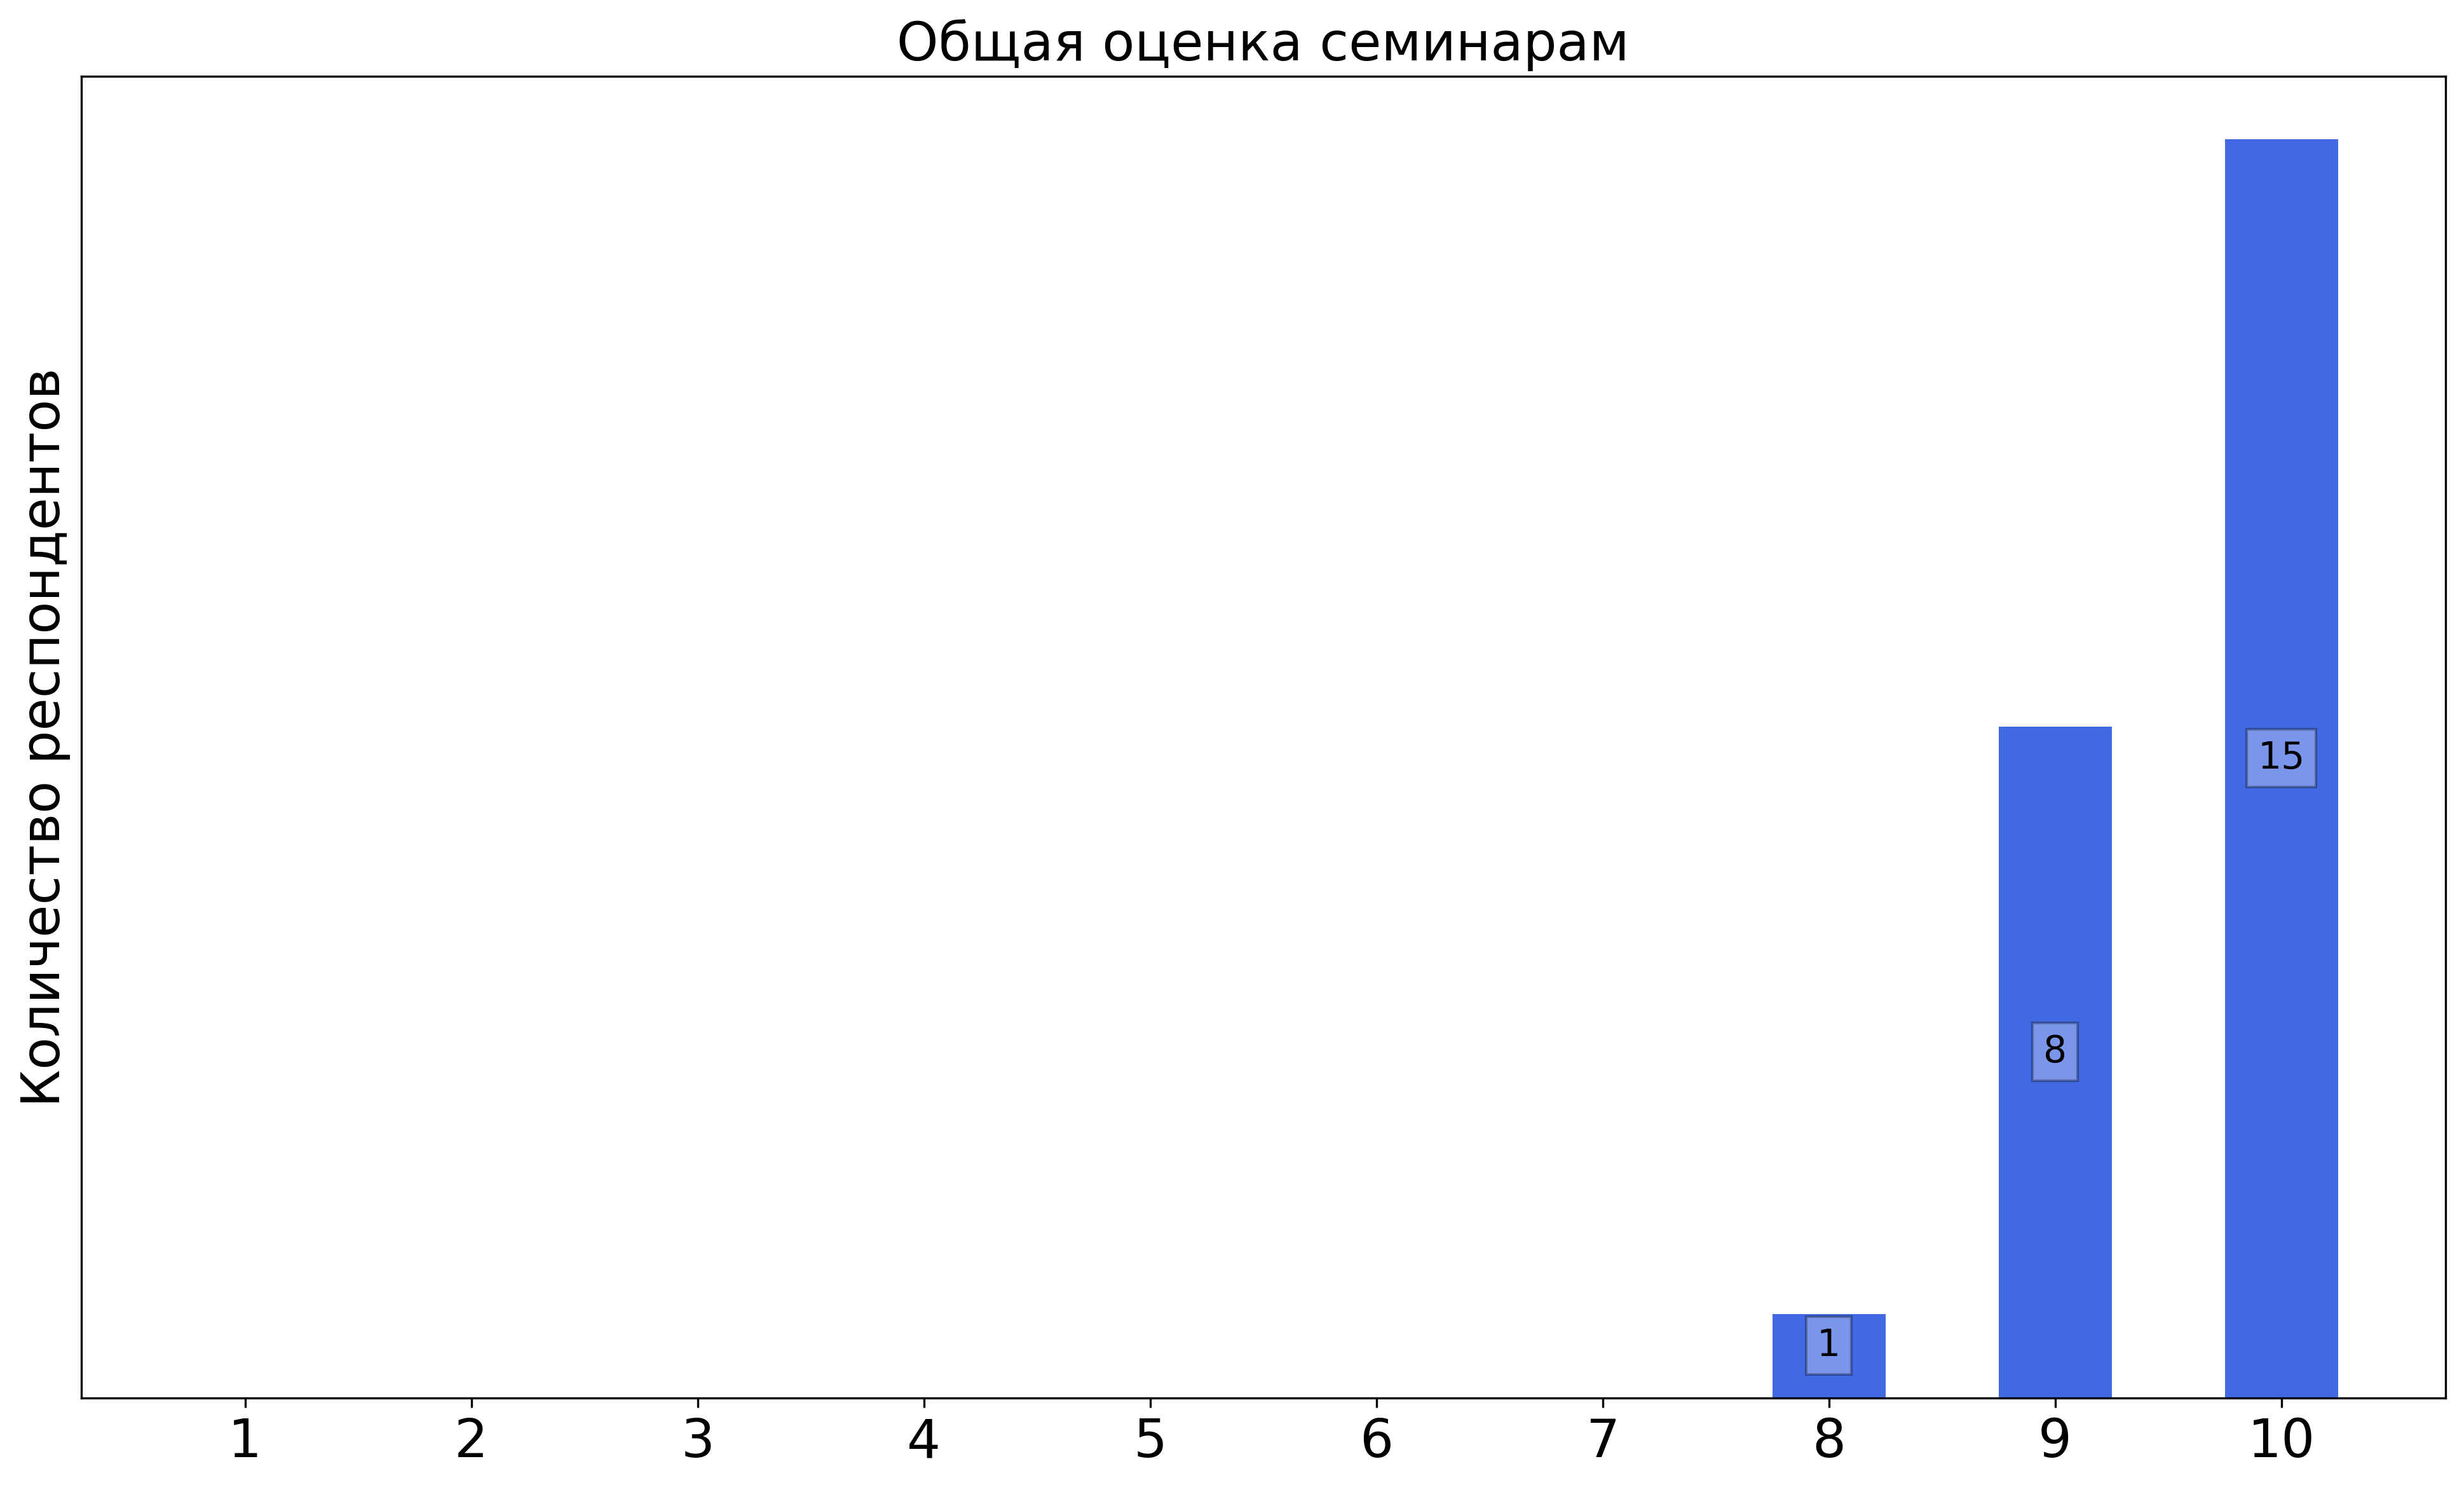
\includegraphics[width=\textwidth]{images/3 course/ТФКП/seminarists-marks-Бунаков А.Э.-3.png}
			\end{subfigure}	
			\caption{Оценки респондентов о качестве преподавания семинаров}
		\end{figure}

		\textbf{Комментарии студентов о семинаристе\protect\footnote{сохранены оригинальные орфография и пунктуация}}
            \begin{commentbox} 
                Объясняет хорошо, только, как по мне, местами очень быстро. Плюс, что успевает разобрать все возможные задачи 
            \end{commentbox} 
        
            \begin{commentbox} 
                Всё классно, решает задачи в большинстве сам, но иногда требует и активности студентов 
            \end{commentbox} 
        
            \begin{commentbox} 
                Очень понятные объяснения с быстрой проверкой. 
            \end{commentbox} 
        
            \begin{commentbox} 
                Претензий нет, исполнение на высшем уровне. 
            \end{commentbox} 
        
            \begin{commentbox} 
                Отличные семинары, все очень понятно. Андрей Эрикович всегда готов к семинару, разбирает полезные задачи, дает теоретическую справку. Самые полезные семинары в моей жизни 
            \end{commentbox} 
        
            \begin{commentbox} 
                У данного преподавателя задачи разобираются ключевые задачи программы, что снова позволяет с легкостью разобраться в материале. Возможно иногда разбор ведётся слишком быстро, но с помощью дополнительных вопросов можно разобраться во всём и снизить темп повествования. 
            \end{commentbox} 
        
            \begin{commentbox} 
                Очень хорошо и эффективно велись семинары 
            \end{commentbox} 
        
            \begin{commentbox} 
                Бунаков хорош, как семенарист. Готов пояснить непонятные моменты без снабизма, идёт на небольшие уступки во время сдачи (можно принести ДЗ в течении неделеи без потери баллов). Даёт возможность повысить оценку за КР на балл.  
            \end{commentbox} 
        
            \begin{commentbox} 
                На семинарах предлагались небольшие выжимки из теории и давалось все необходимое для успешного решения задач, так что написание контрольных было делом техники. Задания и контрольные проверялись в кратчайшие сроки. 
            \end{commentbox} 
        
            \begin{commentbox} 
                Семинары у Бунакова просто отличные! Система оценки хорошая и посильная. Зашаривает замечательно, интересовался, понимаем ли мы его, если нет - объяснял по-другому. 10/10 
            \end{commentbox} 


    \subsubsection{Отзыв студентов о семинарах. Семинарист: Дубинская В.Ю.}
		\begin{figure}[H]
			\centering
			\begin{subfigure}[b]{0.45\textwidth}
				\centering
				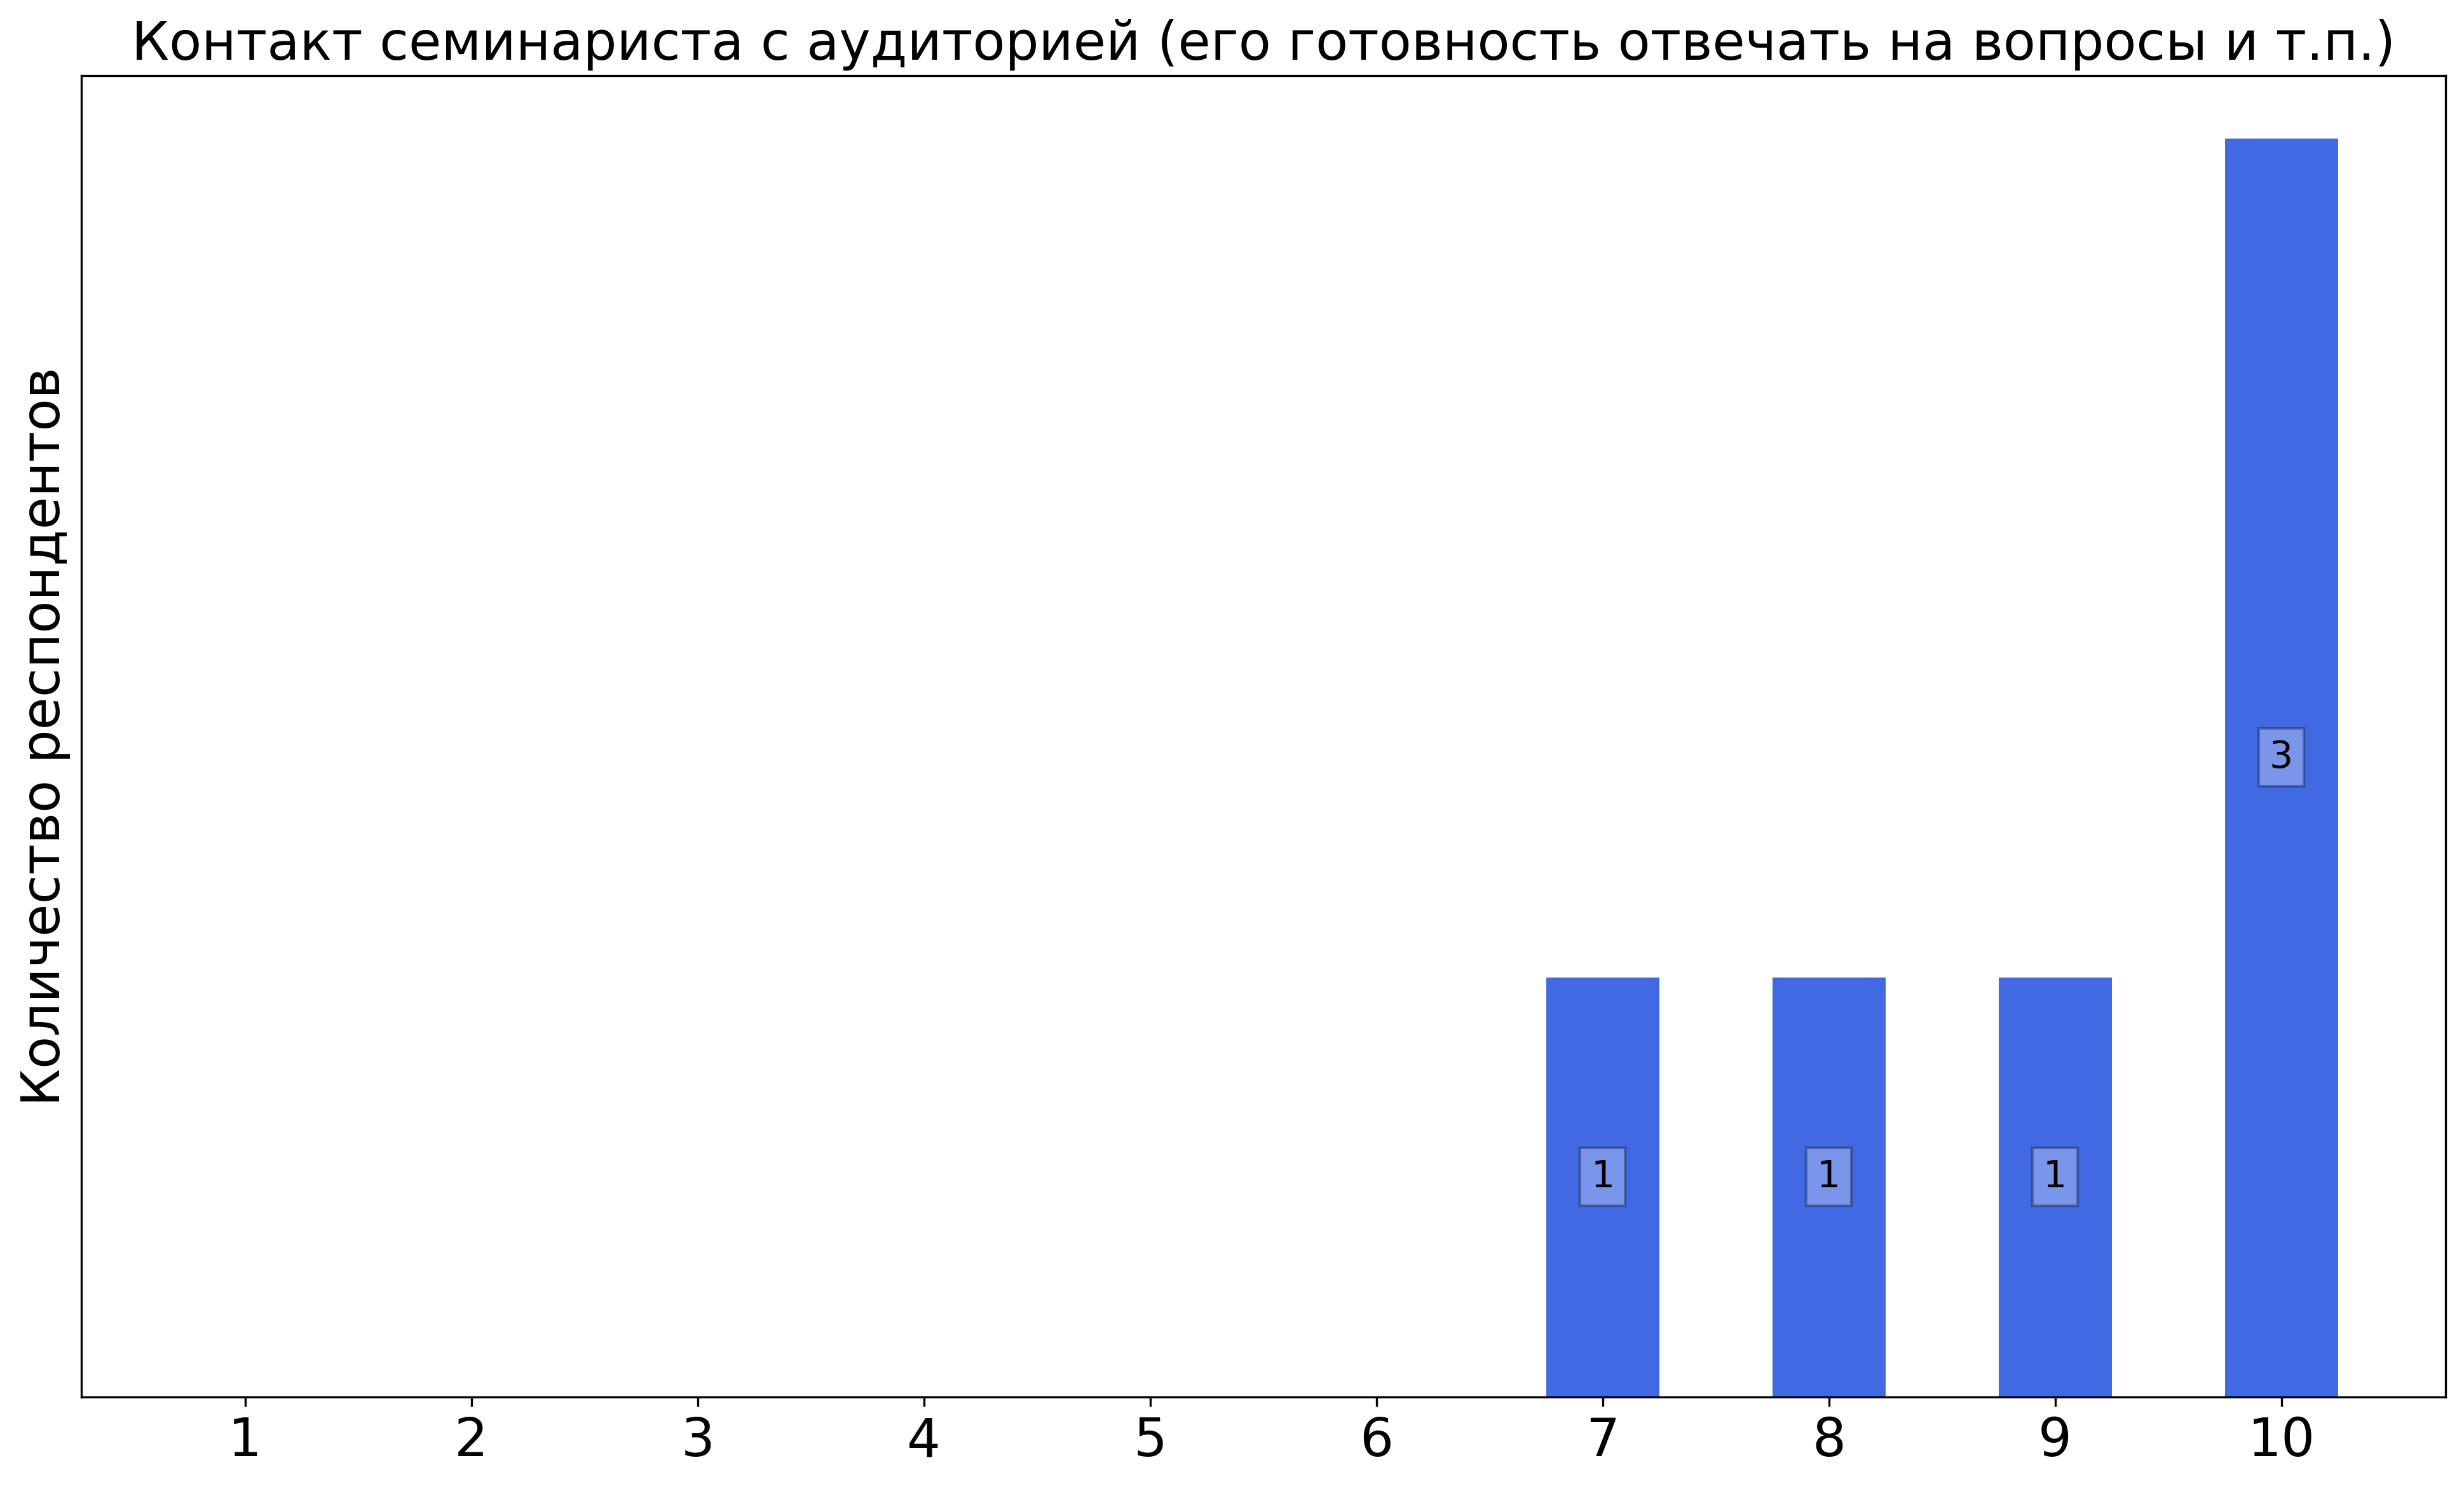
\includegraphics[width=\textwidth]{images/3 course/ТФКП/seminarists-marks-Дубинская В.Ю.-0.png}
			\end{subfigure}
			\begin{subfigure}[b]{0.45\textwidth}
				\centering
				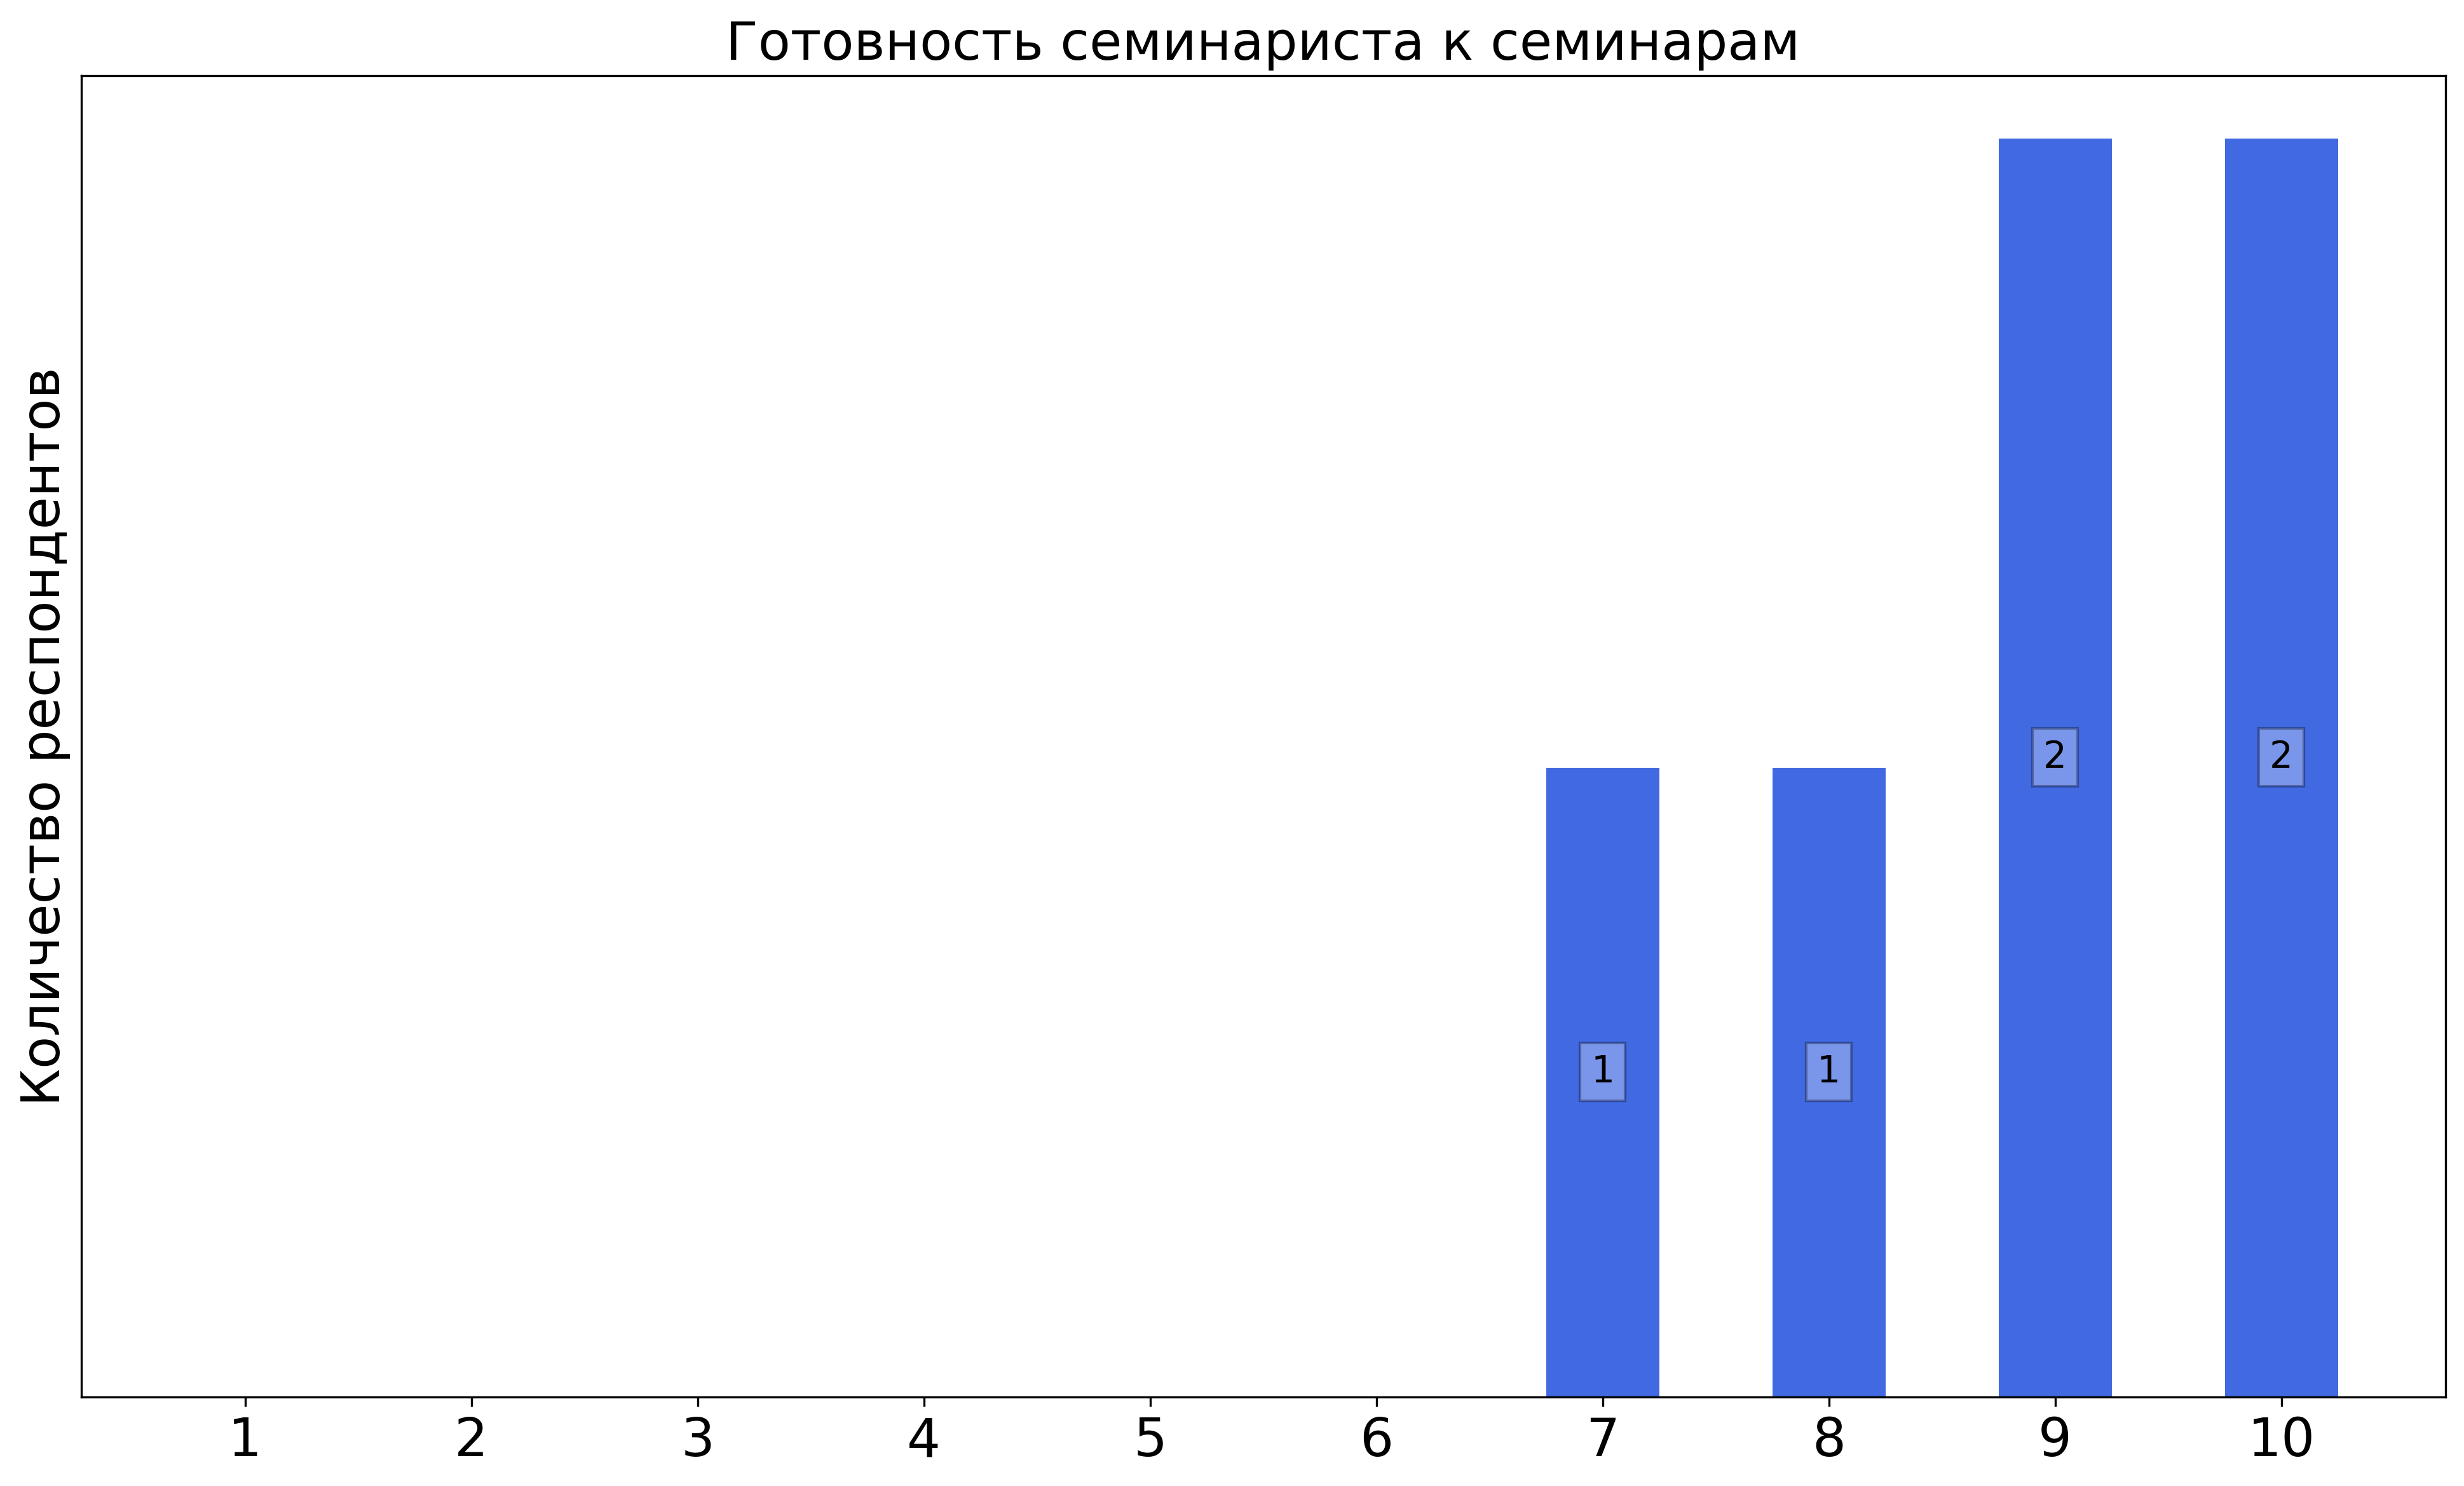
\includegraphics[width=\textwidth]{images/3 course/ТФКП/seminarists-marks-Дубинская В.Ю.-1.png}
			\end{subfigure}
			\begin{subfigure}[b]{0.45\textwidth}
				\centering
				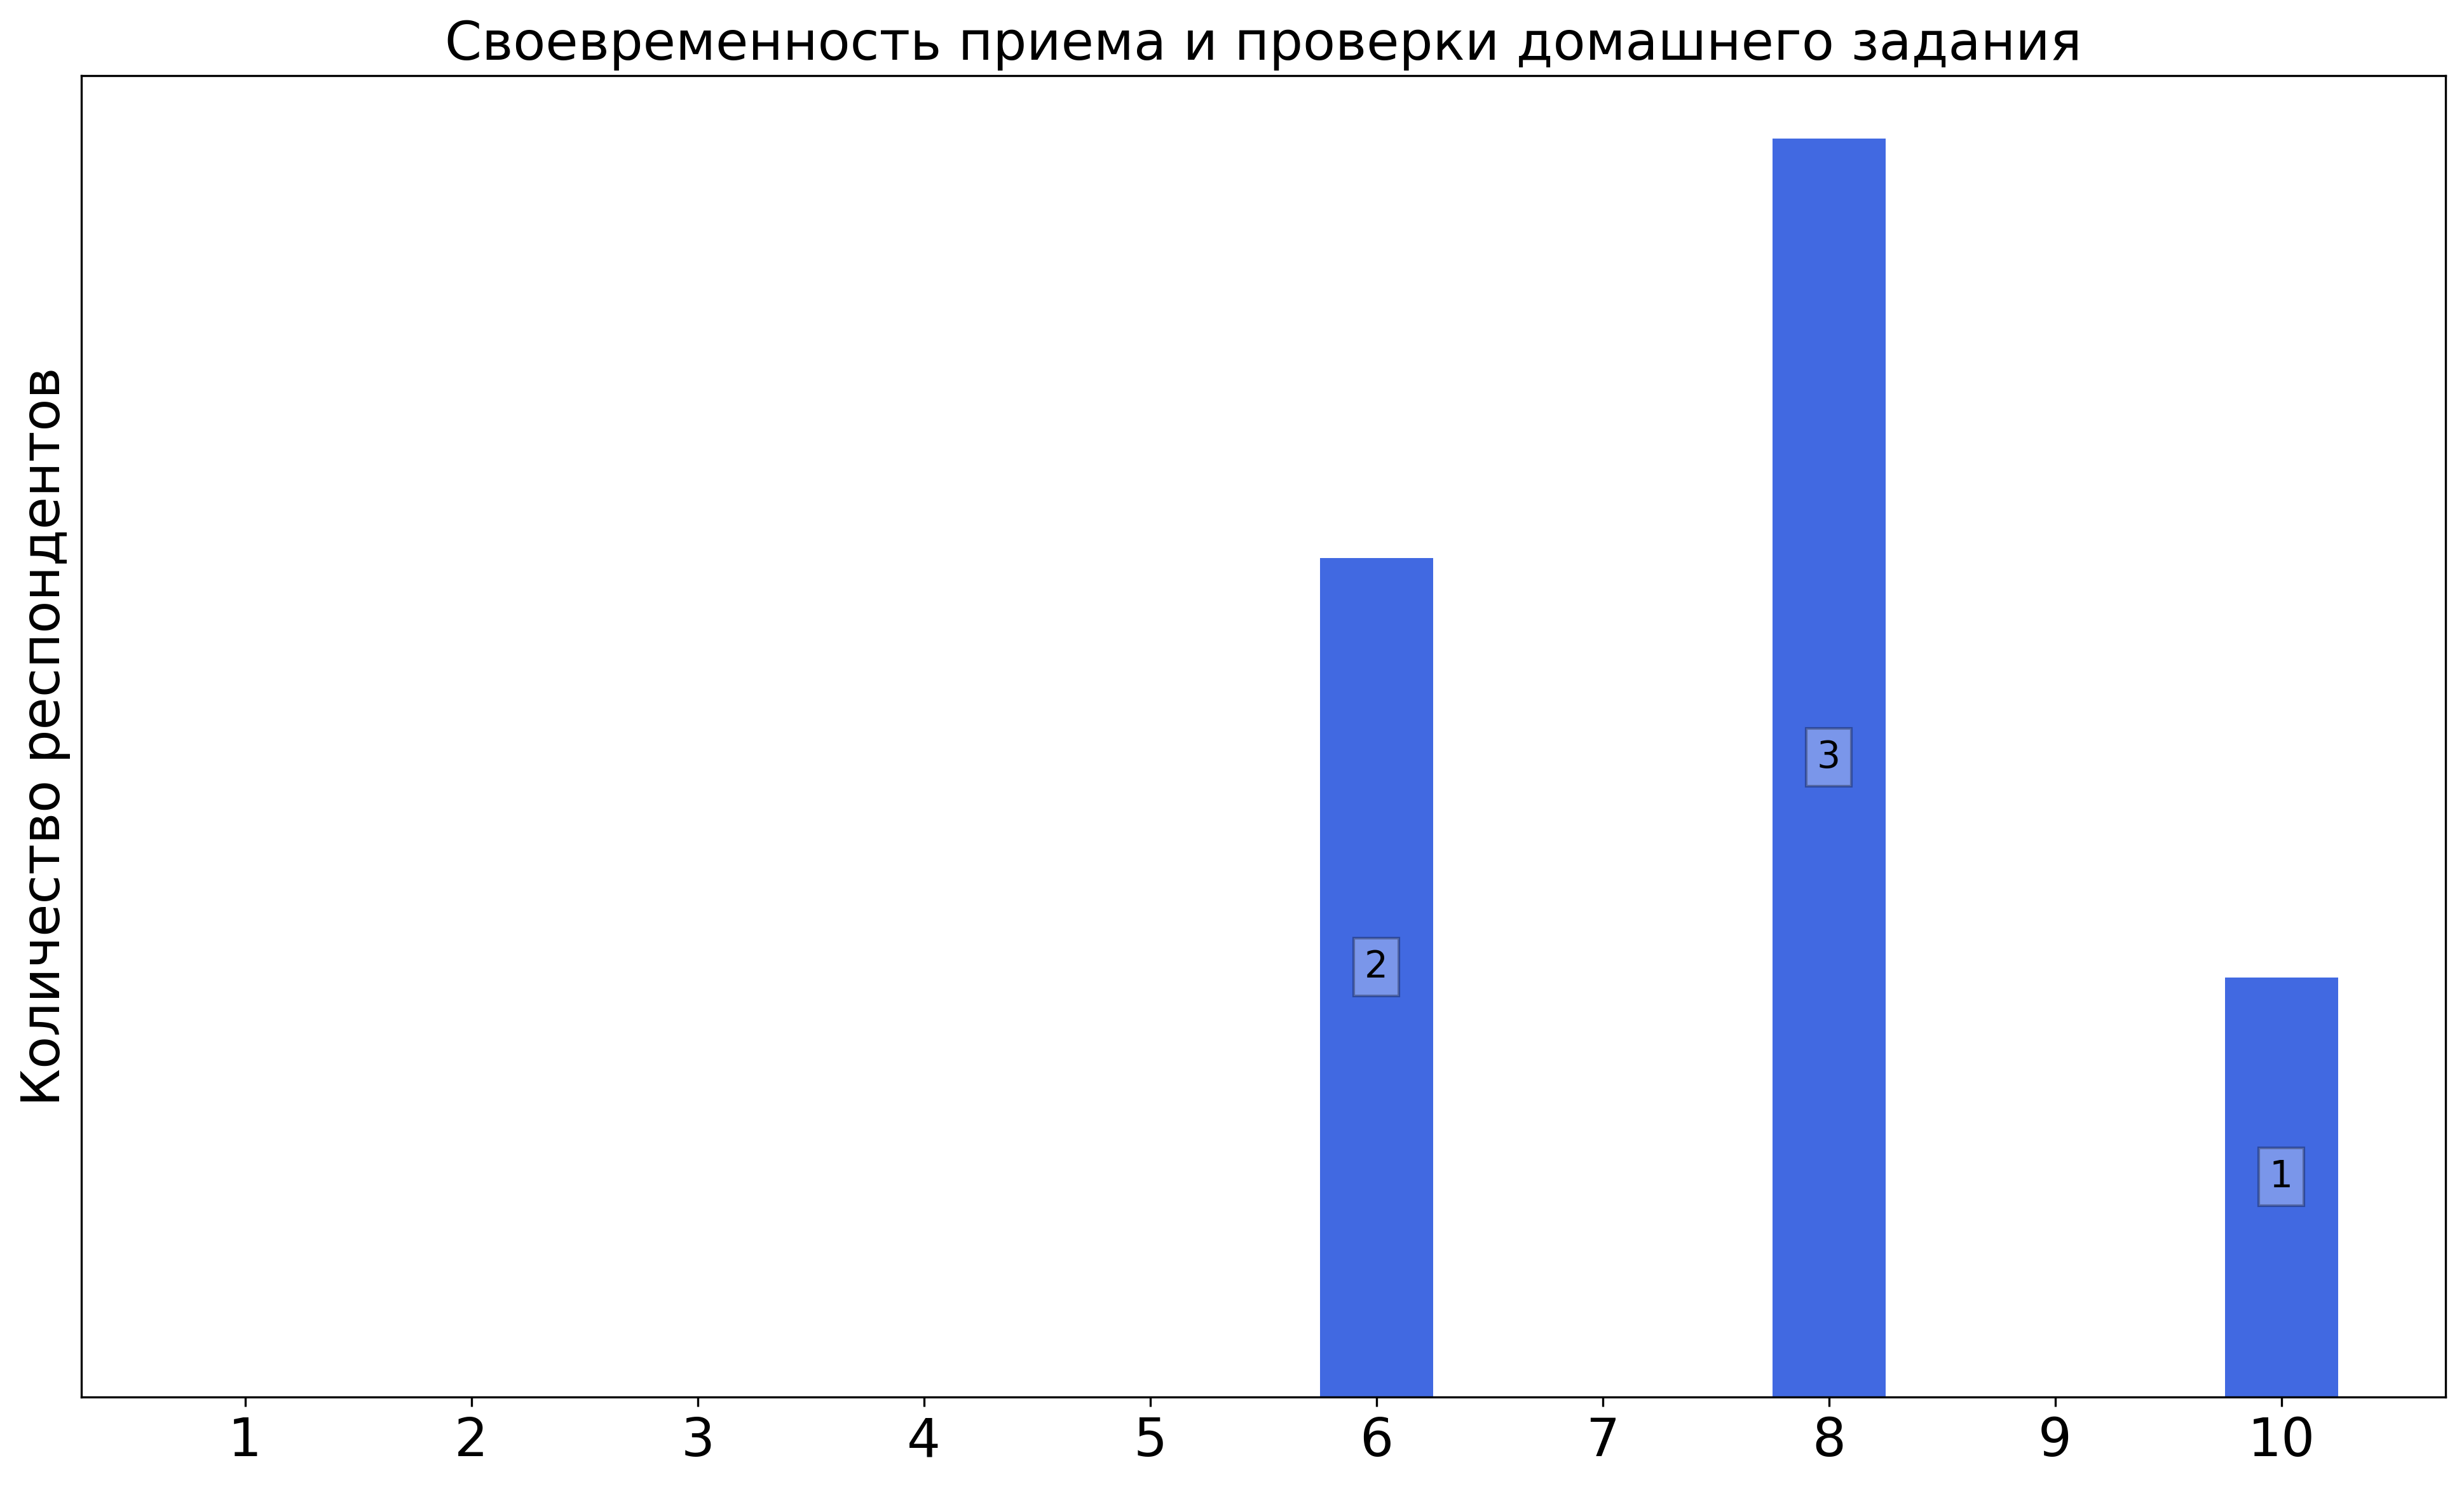
\includegraphics[width=\textwidth]{images/3 course/ТФКП/seminarists-marks-Дубинская В.Ю.-2.png}
			\end{subfigure}
			\begin{subfigure}[b]{0.45\textwidth}
				\centering
				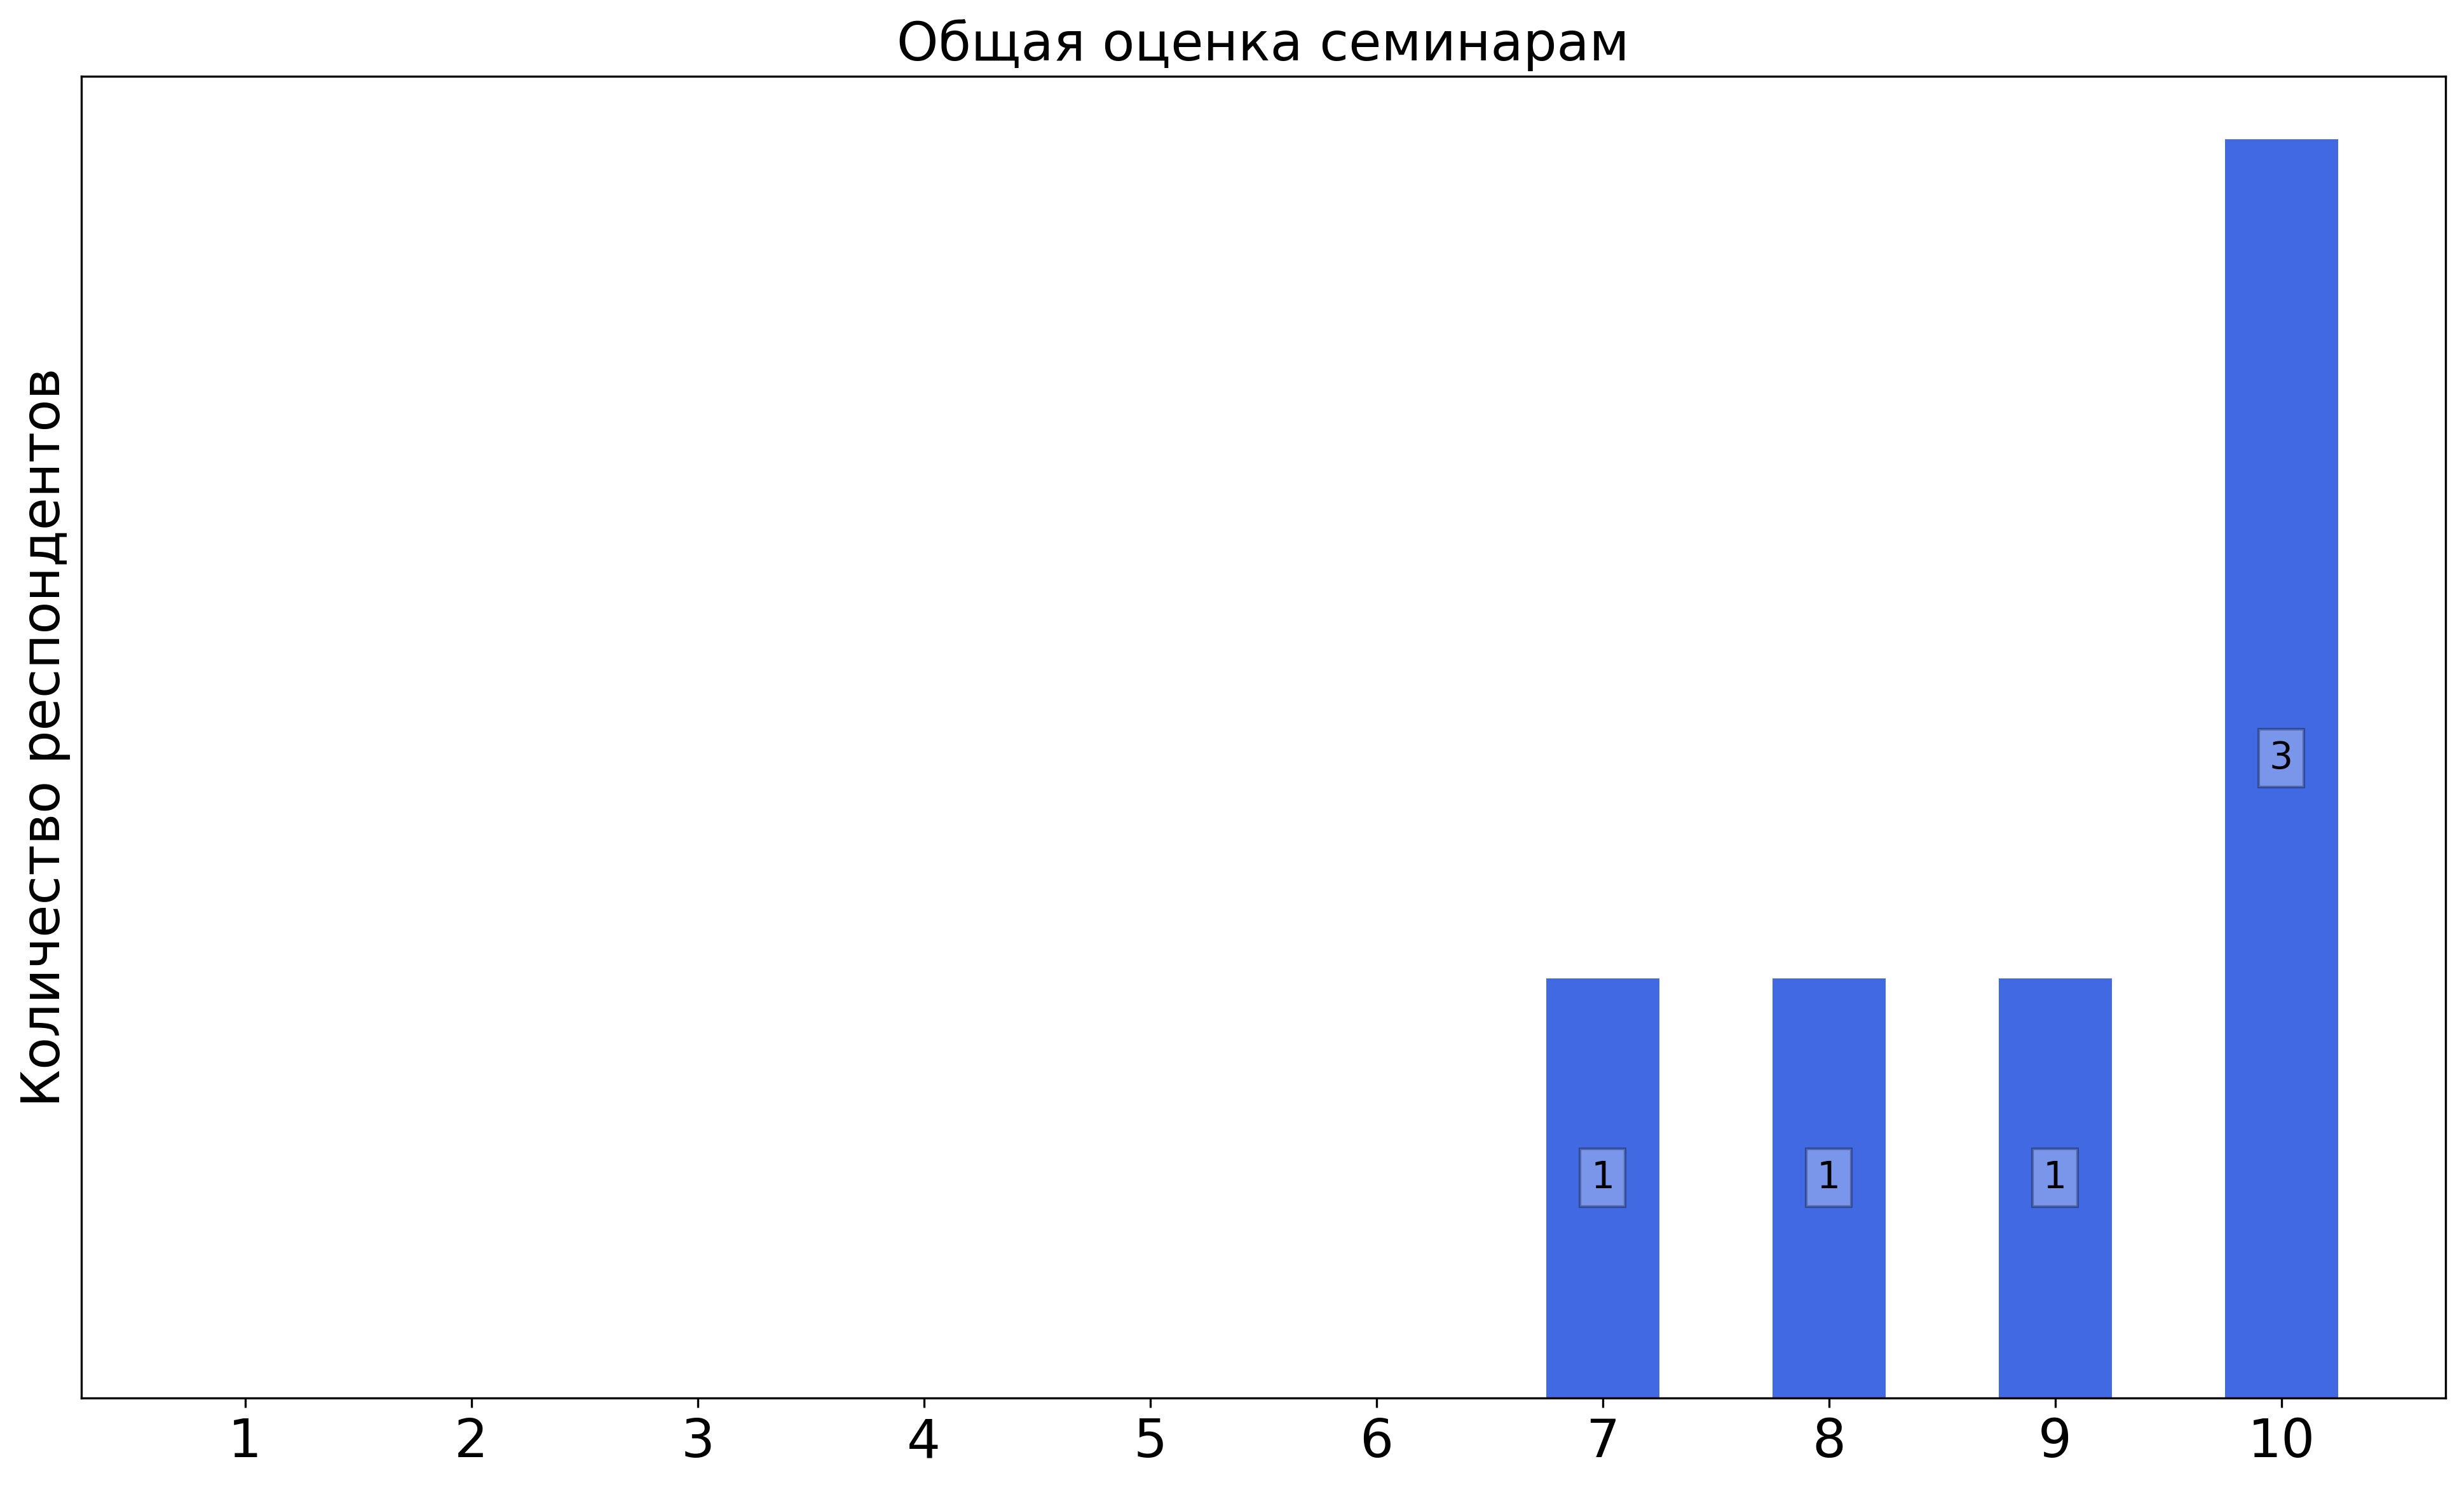
\includegraphics[width=\textwidth]{images/3 course/ТФКП/seminarists-marks-Дубинская В.Ю.-3.png}
			\end{subfigure}	
			\caption{Оценки респондентов о качестве преподавания семинаров}
		\end{figure}

		\textbf{Комментарии студентов о семинаристе\protect\footnote{сохранены оригинальные орфография и пунктуация}}
            \begin{commentbox} 
                Дубинская компетентный семинарист, хорошо и понятно объясняла, если что-то было неясно 
            \end{commentbox} 
        
            \begin{commentbox} 
                Вера Юльевна прекрасный преподаватель. Все расшарит и оценкой не обидит. ТФКП было в удовольствие 
            \end{commentbox} 
        
            \begin{commentbox} 
                Хорошо. Старается скорее разложить по полочкам как все работает, а не научить тупо считать, но из-за этого иногда может вскипеть мозг. Домашку не успевает проверять, но есть и плюс в виде халявных баллов за дз. КР смотрит нормально, больше. пользу студента. 
            \end{commentbox} 


    \subsubsection{Отзыв студентов о семинарах. Семинарист: Киреенков А.А.}
        \begin{figure}[H]
            \centering
            \begin{subfigure}[b]{0.45\textwidth}
                \centering
                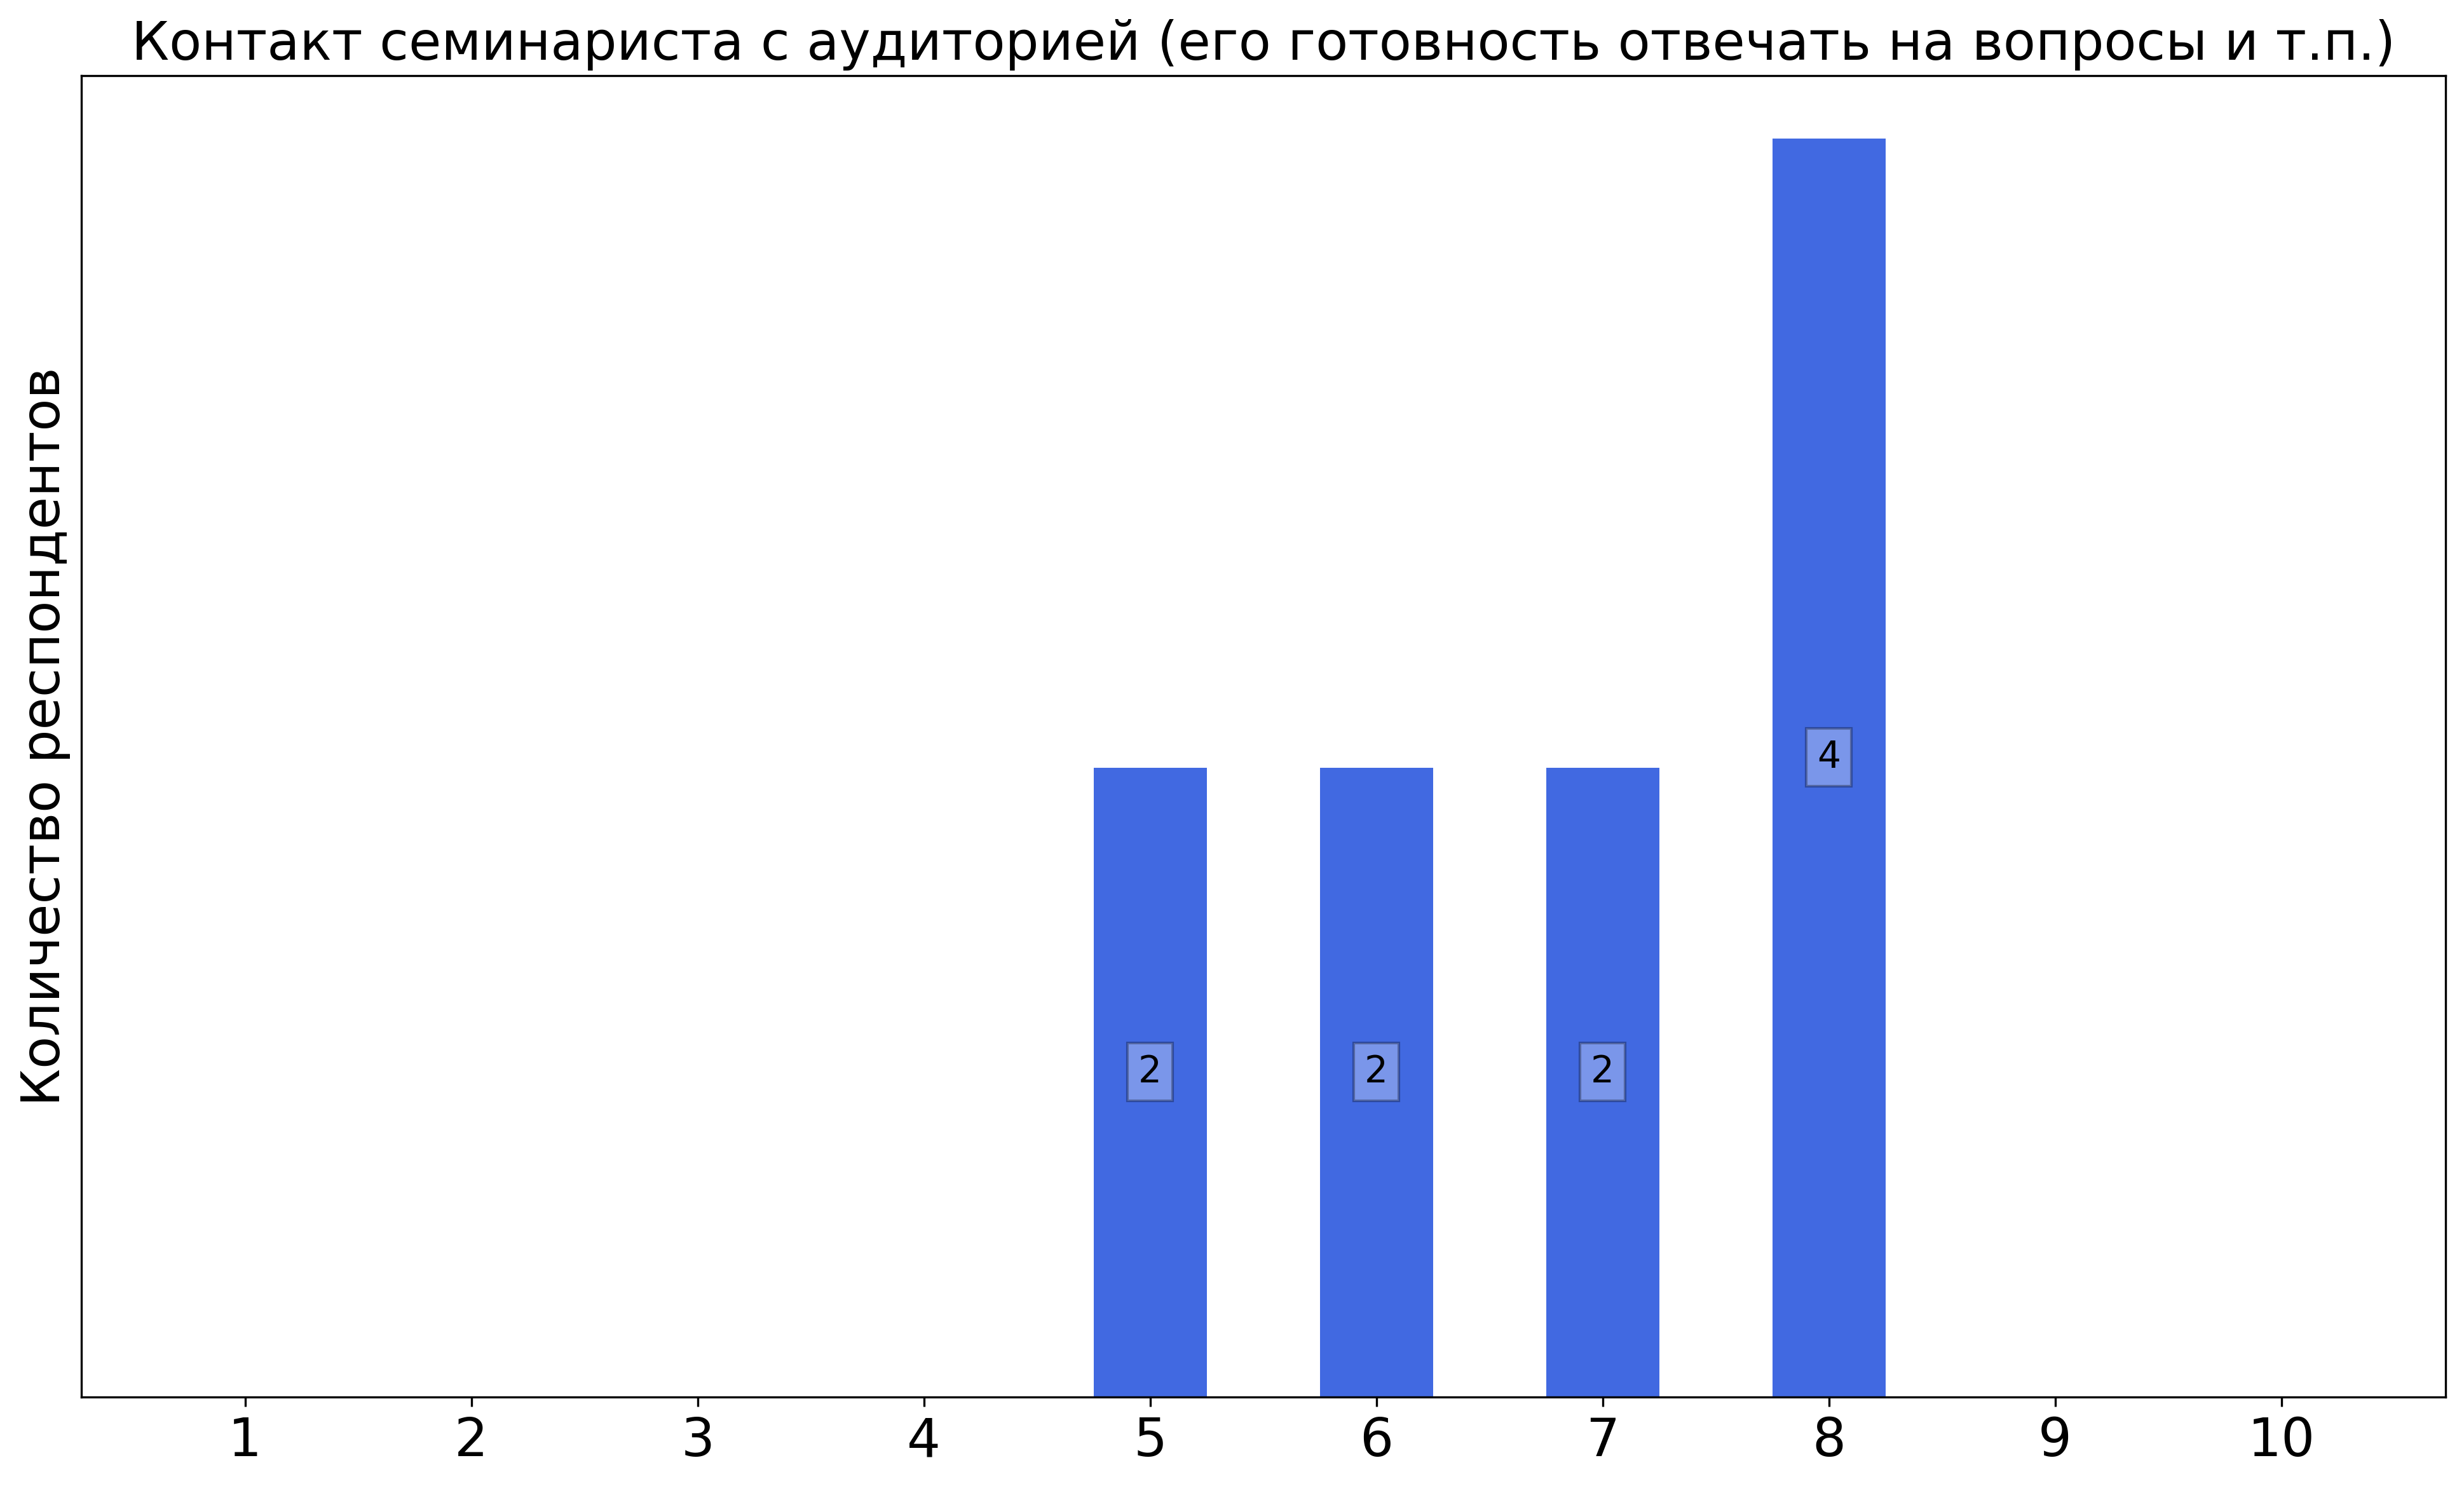
\includegraphics[width=\textwidth]{images/3 course/ТФКП/seminarists-marks-Киреенков А.А.-0.png}
            \end{subfigure}
            \begin{subfigure}[b]{0.45\textwidth}
                \centering
                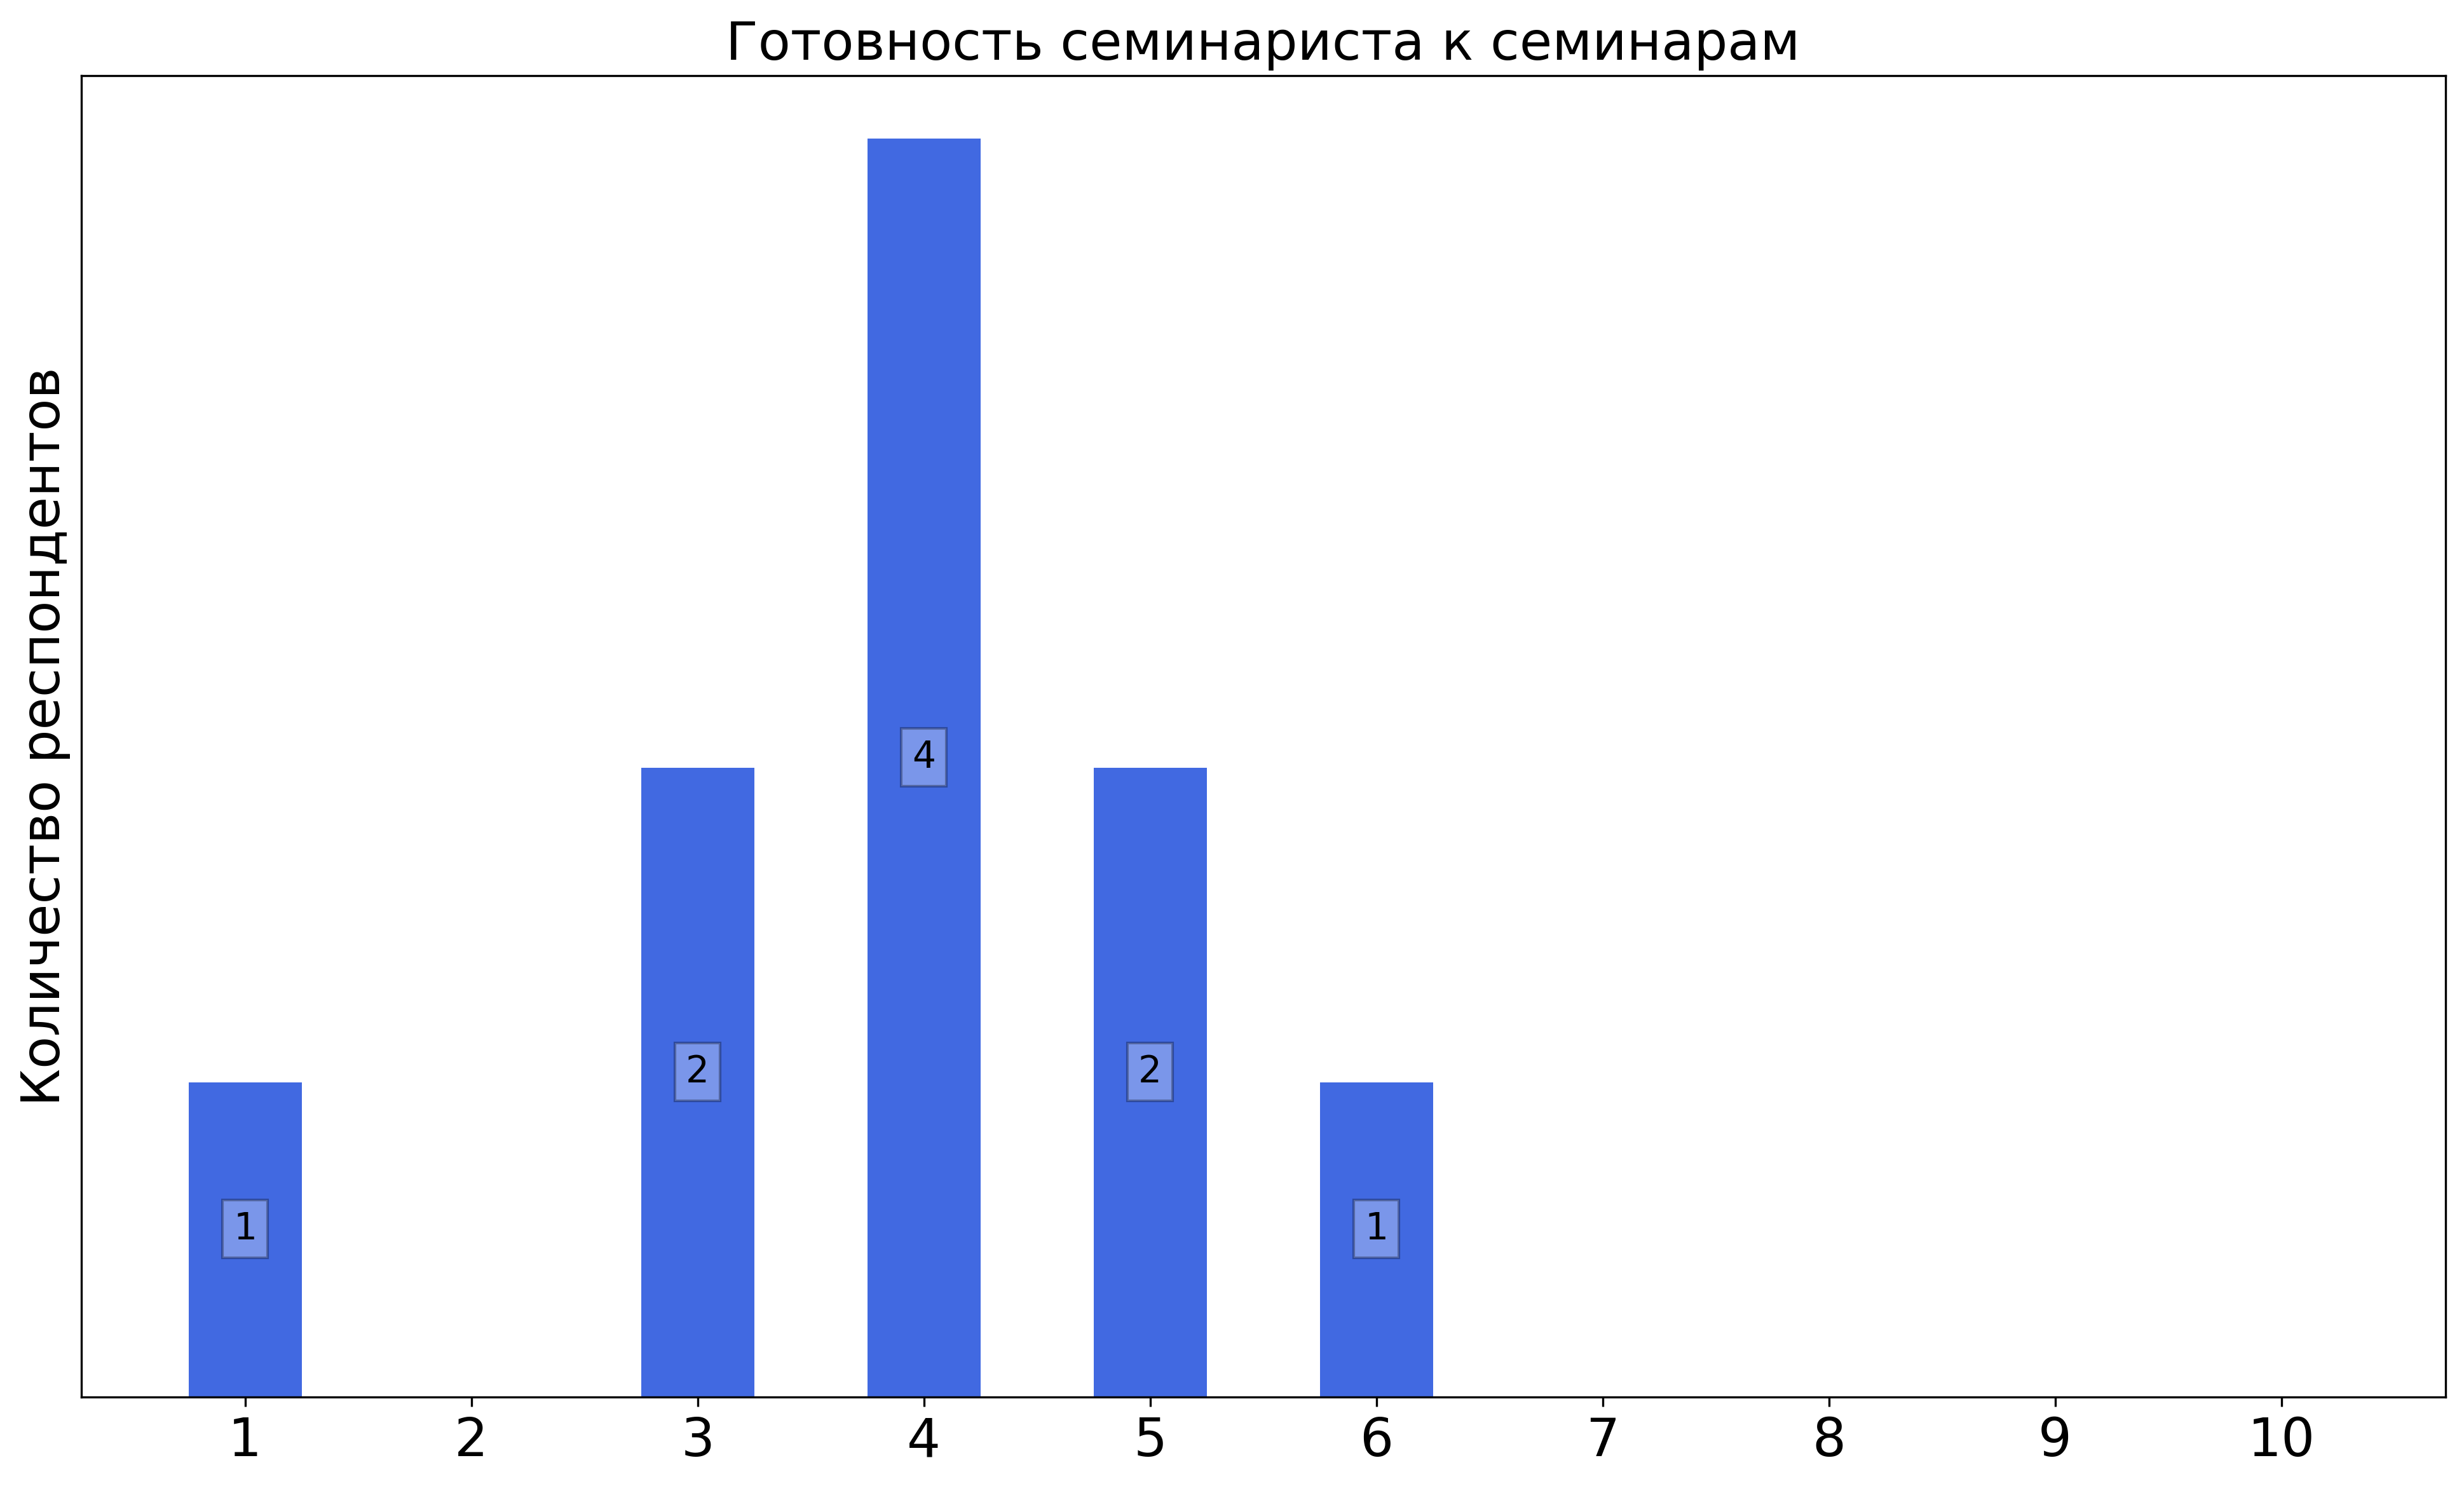
\includegraphics[width=\textwidth]{images/3 course/ТФКП/seminarists-marks-Киреенков А.А.-1.png}
            \end{subfigure}
            \begin{subfigure}[b]{0.45\textwidth}
                \centering
                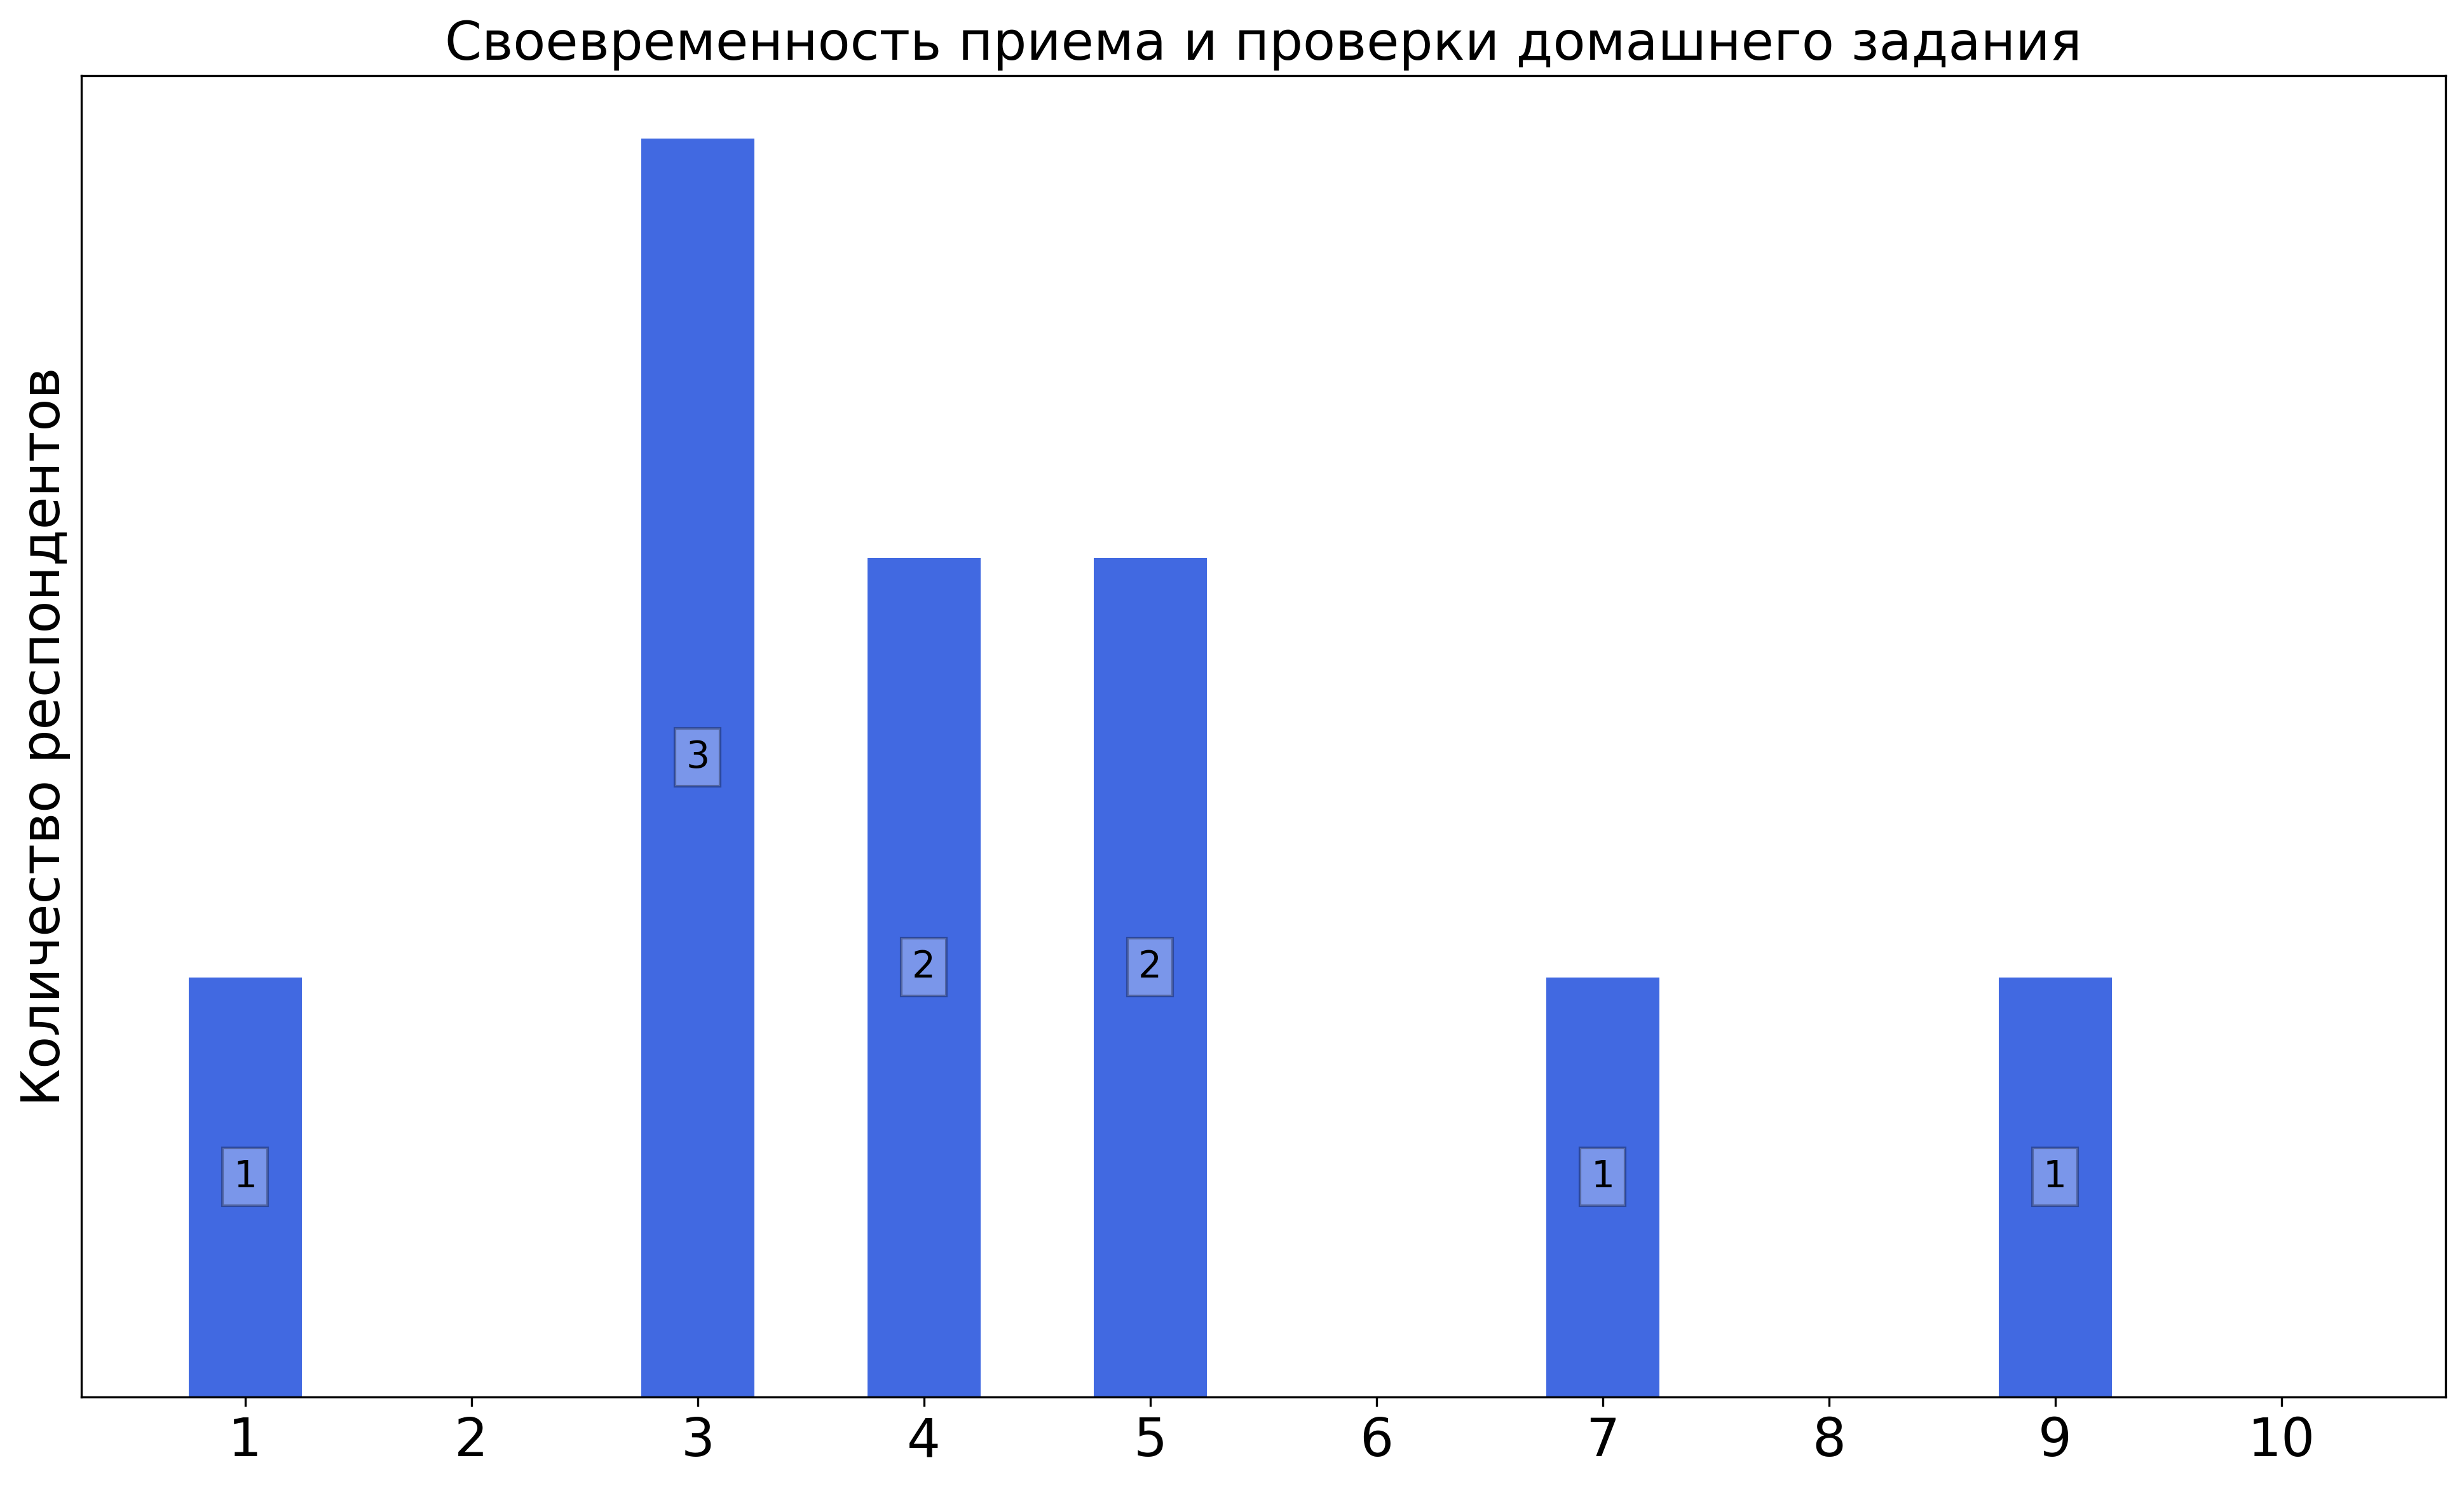
\includegraphics[width=\textwidth]{images/3 course/ТФКП/seminarists-marks-Киреенков А.А.-2.png}
            \end{subfigure}
            \begin{subfigure}[b]{0.45\textwidth}
                \centering
                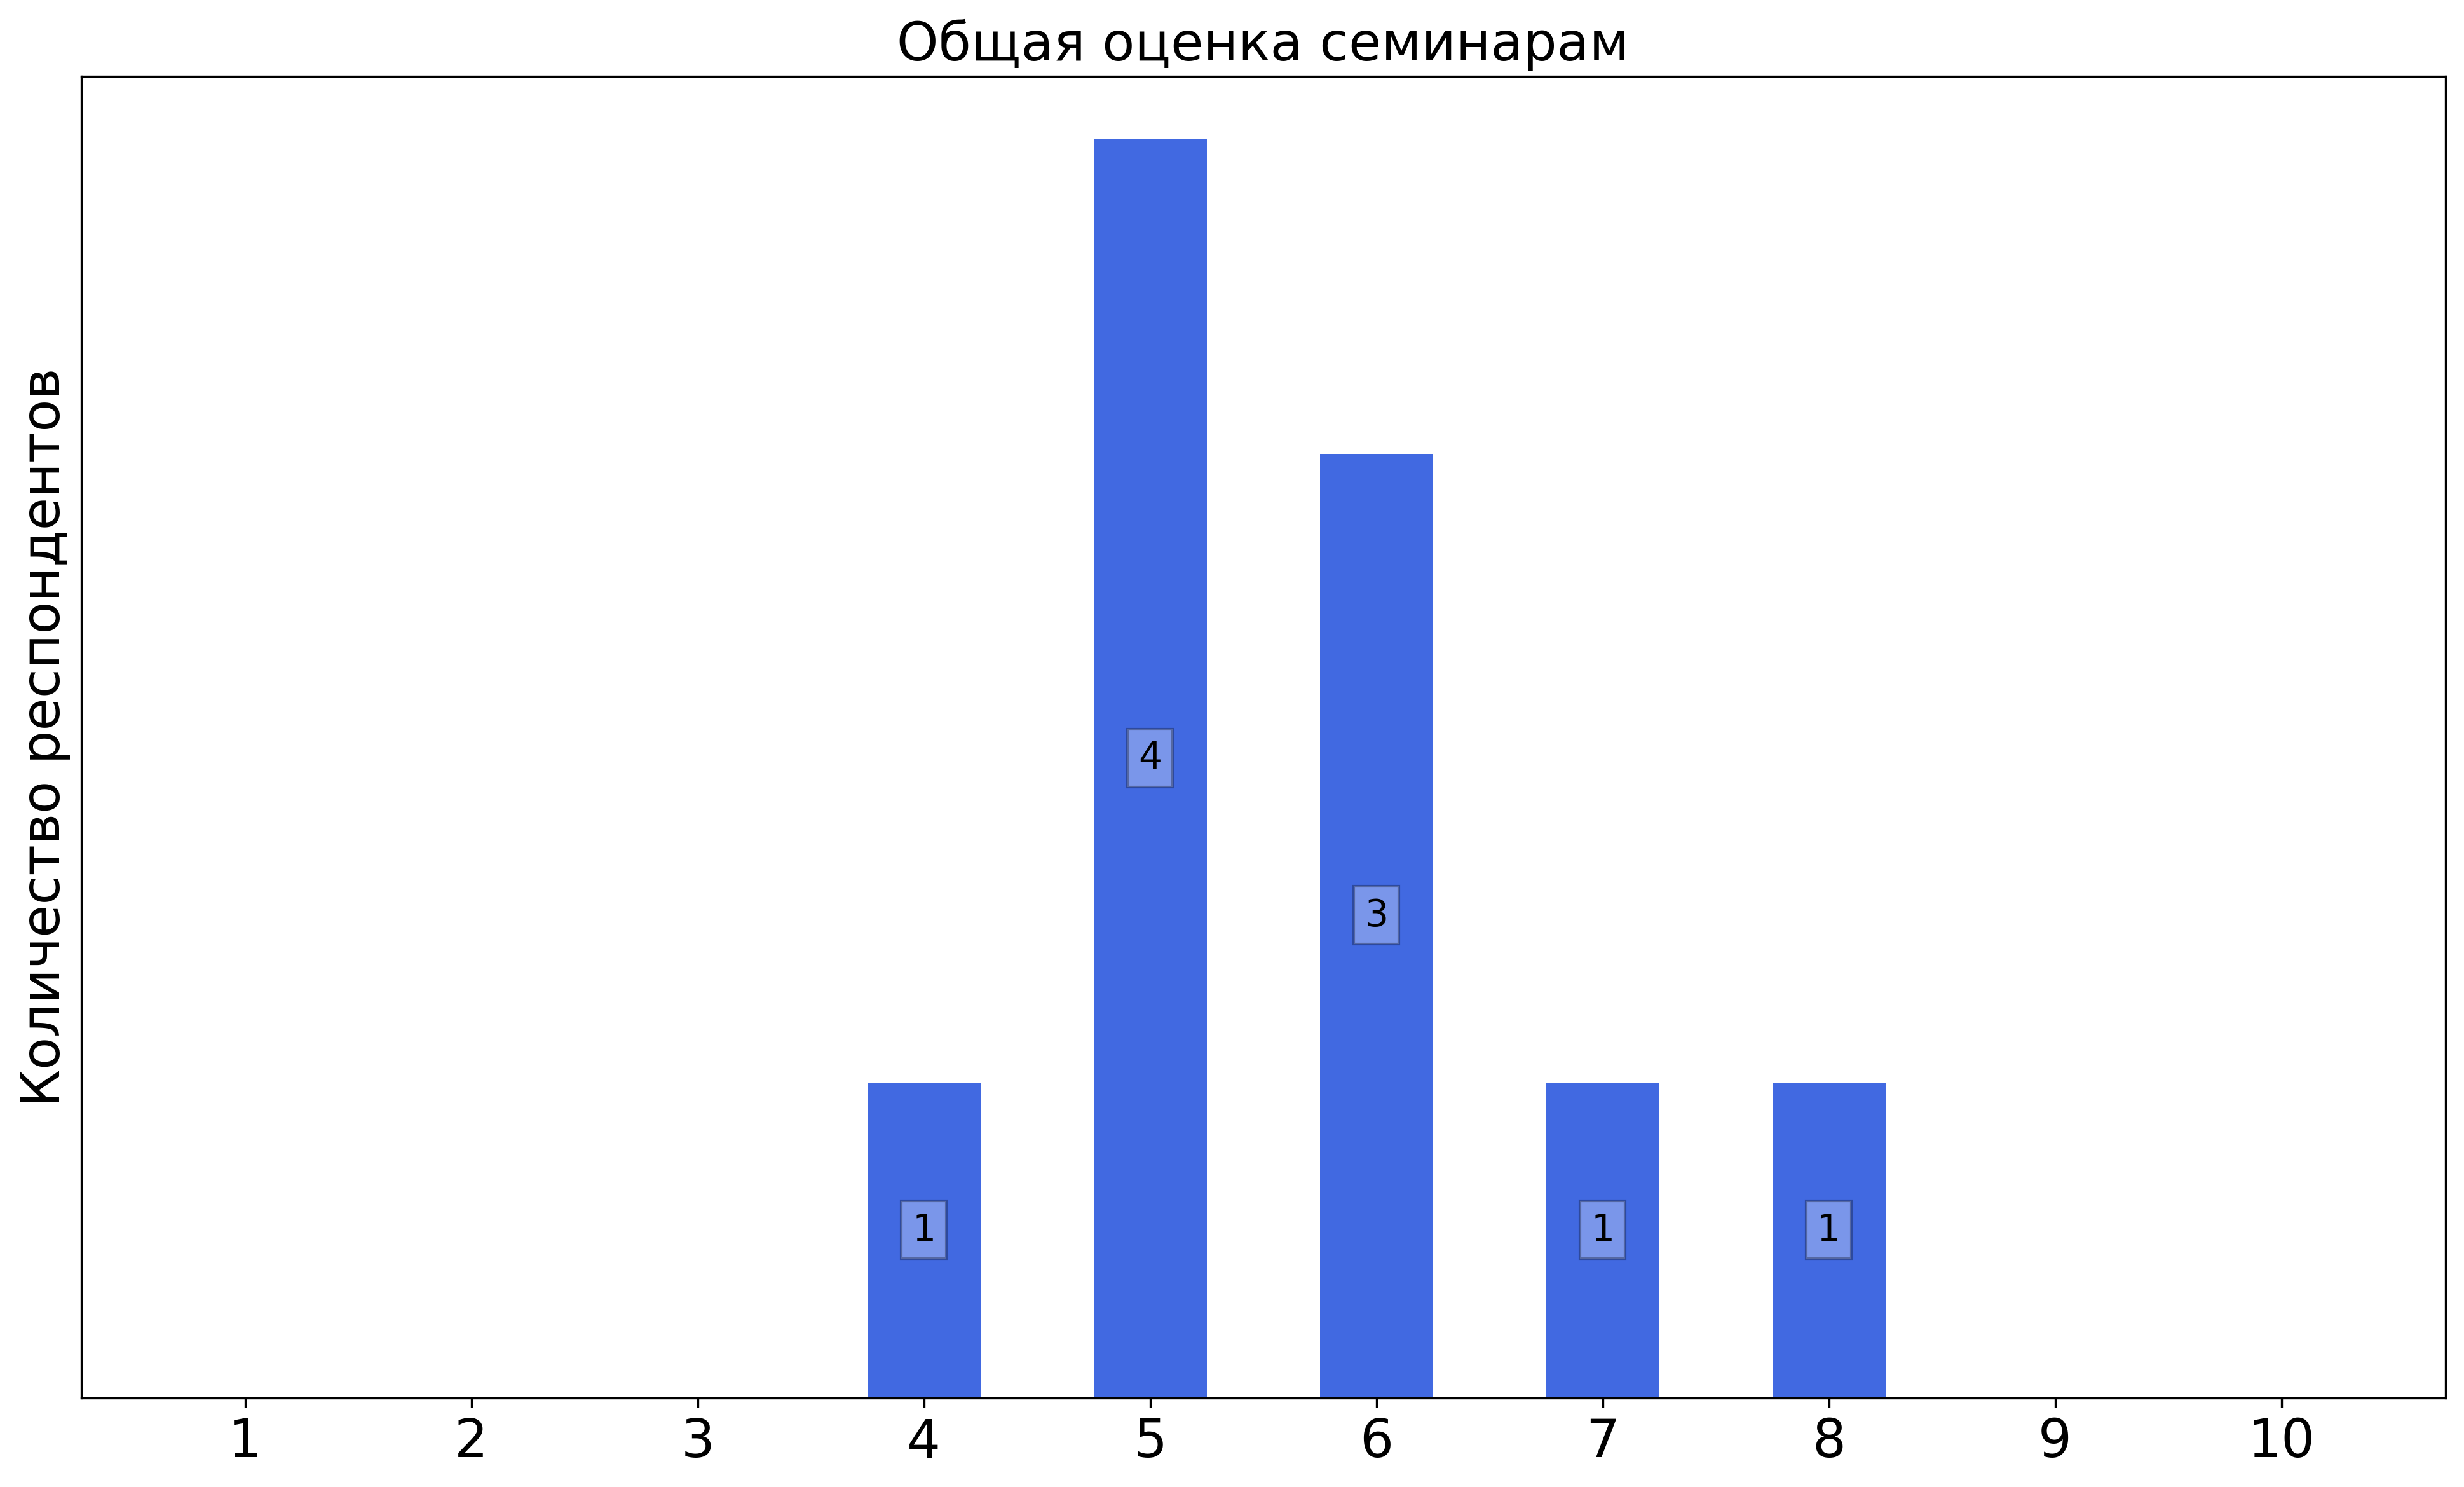
\includegraphics[width=\textwidth]{images/3 course/ТФКП/seminarists-marks-Киреенков А.А.-3.png}
            \end{subfigure}	
            \caption{Оценки респондентов о качестве преподавания семинаров}
        \end{figure}

        \textbf{Комментарии студентов о семинаристе\protect\footnote{сохранены оригинальные орфография и пунктуация}}
            \begin{commentbox} 
                Хороший человек, брс выставляет щедро, но часто опаздывал на семинары, приходил не готовый(часто не знал что нам порешать и сидел искал в планшете), вызывал людей к доске и почти им не помогал решать, на вопросы отвечал, но не всегда развёрнуто. При сдаче заданий объявлял о возможности сдать это же задание сегодня же после пары, что было неудобно так как мы были или не готовы, или у нас были планы/пары в это время, приходилось подстраиваться. Было бы здорово если бы он обсуждал с нами время когда мы можем сдать задание. 
            \end{commentbox} 
        
            \begin{commentbox} 
                Неплохой семинарист, но часто дает задания, которые не знает как решить и в случае неуспеха может даже перейти к другой задаче. Задания для классной работы зачастую смотрит просто в задавальнике прям во время семинара. В общении +- приятный. Контрольные уровня дз, брсом не обижает. В целом задачу семинариста выполняет (все типы задач разобраны), оценивает нормально, но бывают неприятные моменты 
            \end{commentbox} 
        
            \begin{commentbox} 
                Кириенков - прикольный преподаватель, хорошо, что был именно семинаристом, а не принимающим на экзамене) К семинарам почти никогда не был готов, задачи решал через раз (иногда перерешивали задачу по несколько раз, потому что ответ, к которому приходил преподаватель, не сходился с учебником)) ). В общем спасибо за нормальный БРС, в остальном было самообучение)) 
            \end{commentbox} 
        
            \begin{commentbox} 
                В целом приятный семинарист, рассказывает теорию, сам разбирает задачи (иногда вызывает к доске, но в процессе решения помогает), шутит. Из минусов иногда может затупить над задачей, и очень плохо с проверкой контрольных и дз 
            \end{commentbox} 
        
            \begin{commentbox} 
                Не готовится к семинарам вообще, постоянно отвлекается. Постоянно уставший и занятой. Контрольную по первому заданию проверил (лично у меня) только в конце семестра. В целом семинары помогают с решением домашки, не совсем плохие, но отношение у Киреенкова к работе не очень ответсвенное. 
            \end{commentbox} 
        
            \begin{commentbox} 
                Семинарист плохо готовится к семинарам, может по 10 минут искать задачи для решения. Не всегда адекватно отвечает на вопросы на семинаре.  
            \end{commentbox} 
        
            \begin{commentbox} 
                Семинарист халявный, на семинарах шутит, иногда даже смешно. На этом плюсы заканчиваются. Сложилось впечатление, что сам он не особо шарит за предмет, или просто очень плохо умеет объяснять 
            \end{commentbox} 


    \subsubsection{Отзыв студентов о семинарах. Семинарист: Лопушански М.С.}
		\begin{figure}[H]
			\centering
			\begin{subfigure}[b]{0.45\textwidth}
				\centering
				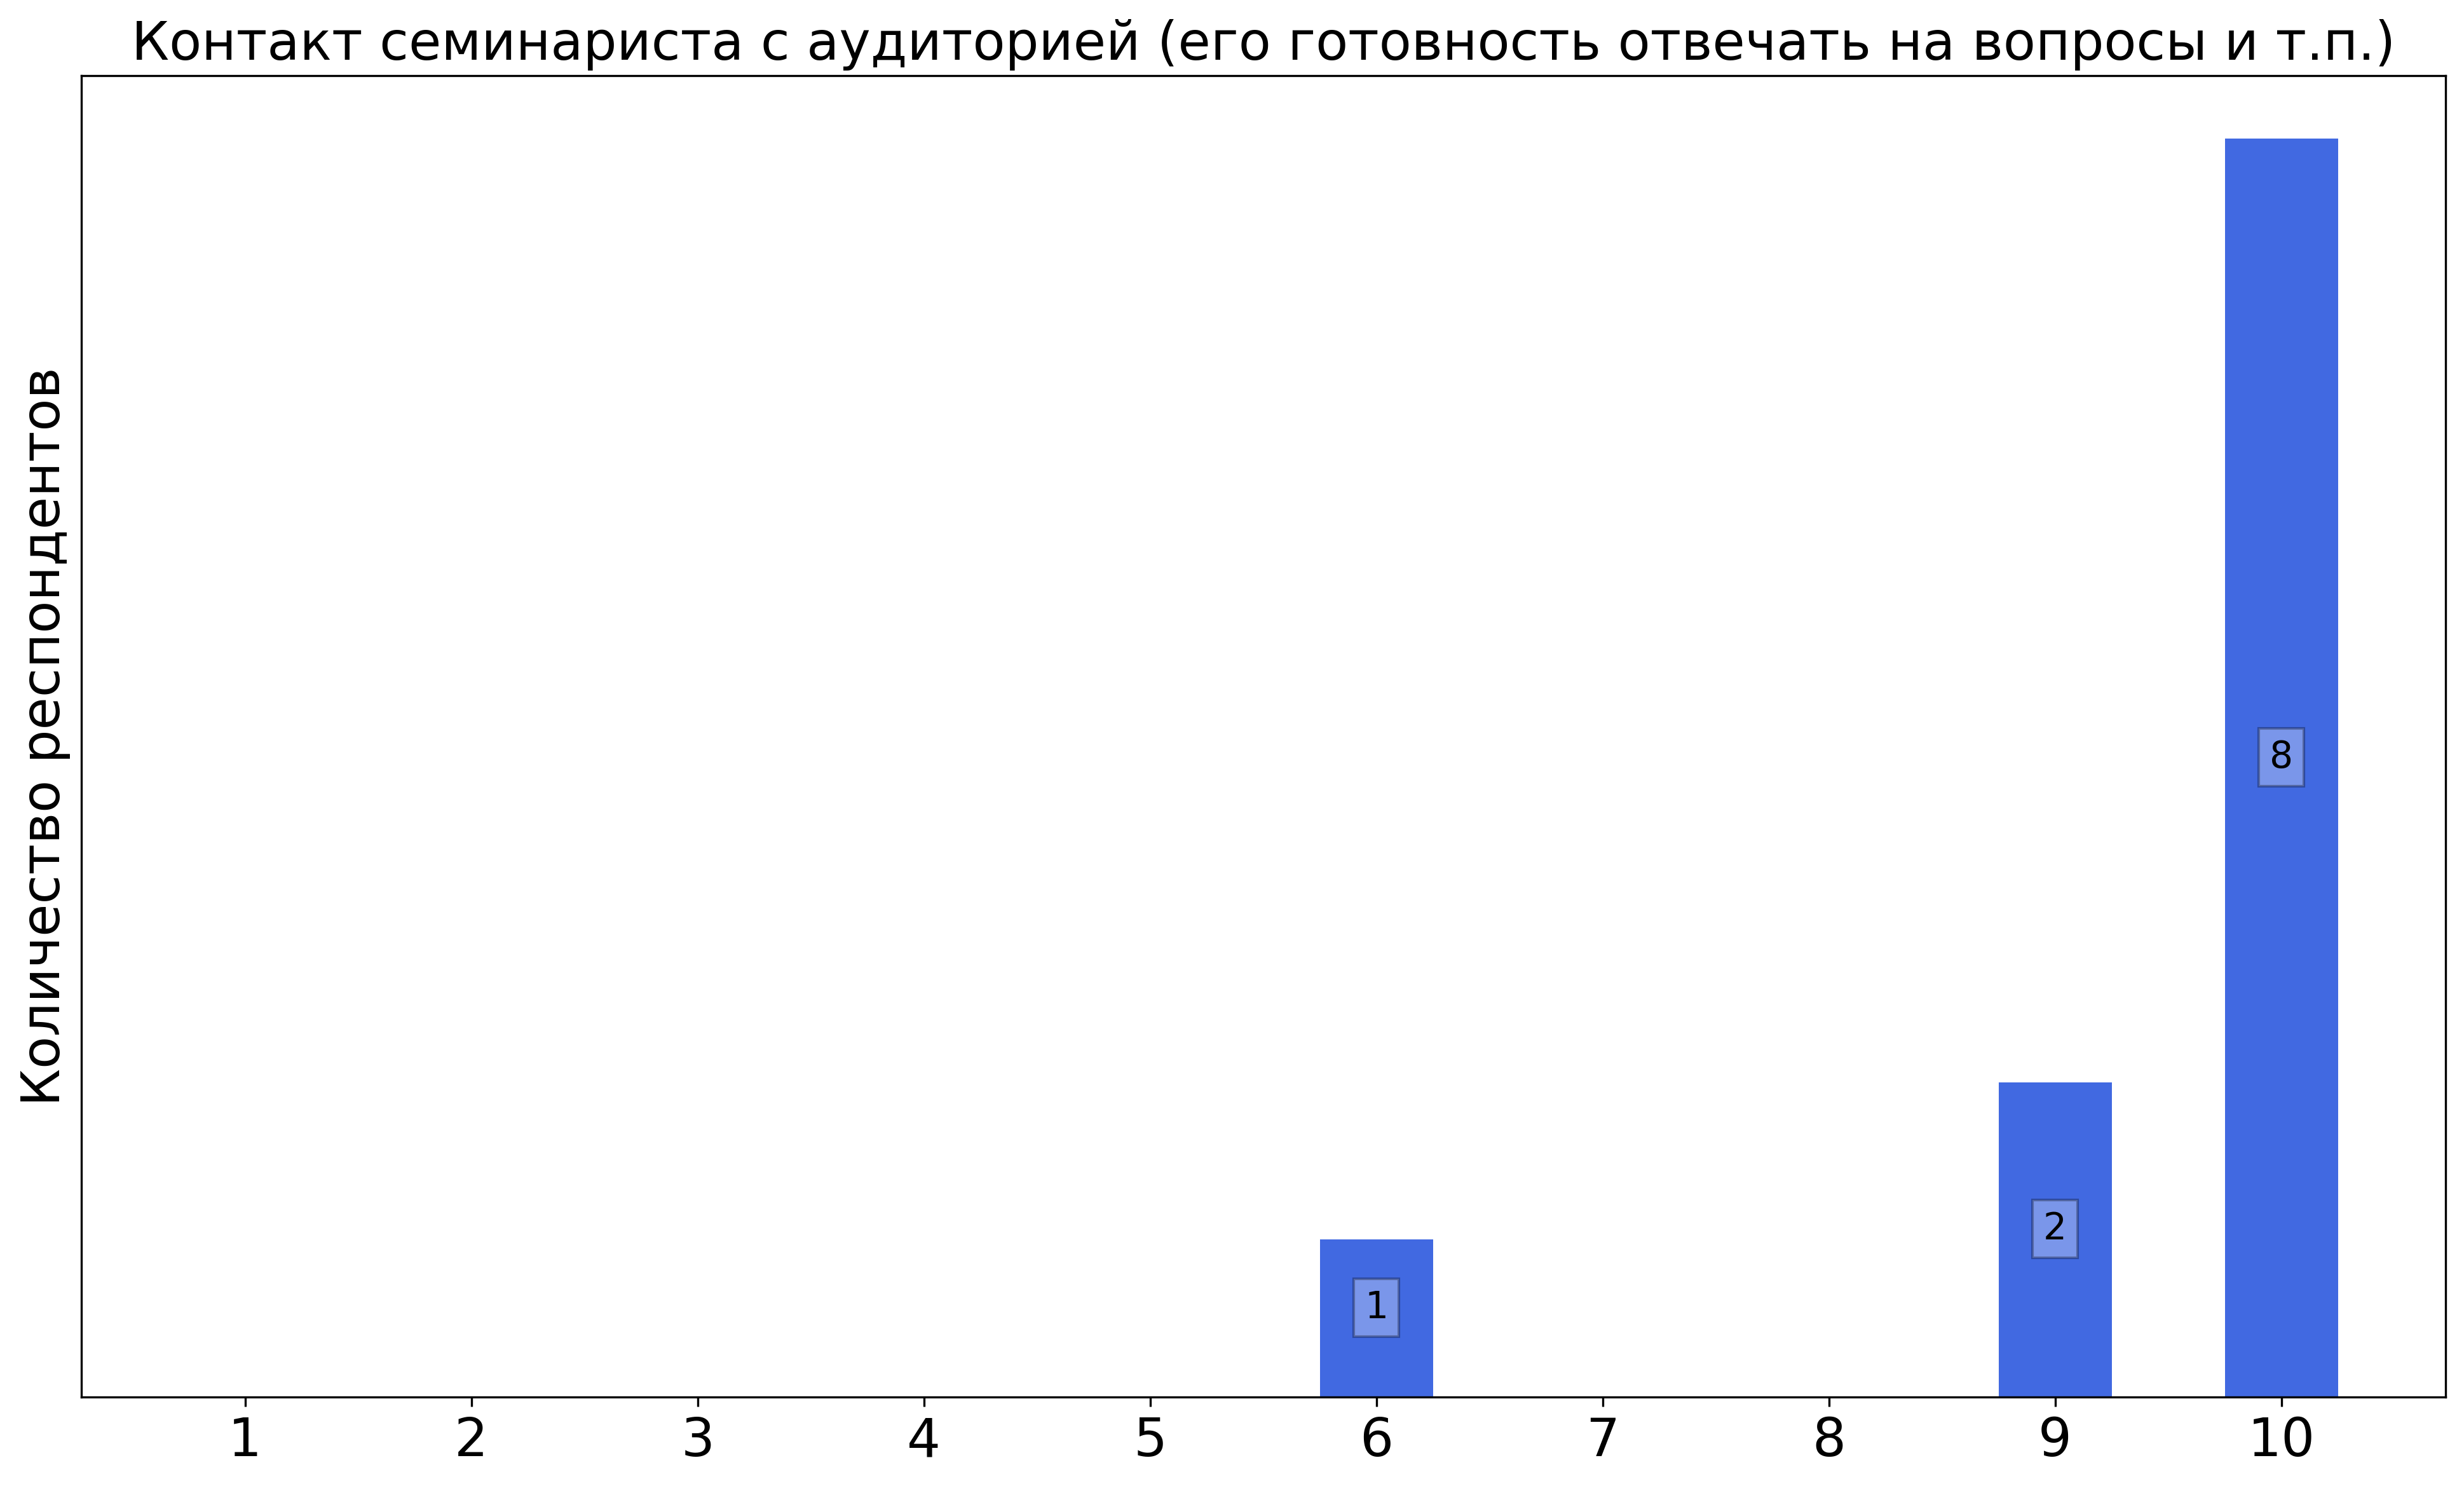
\includegraphics[width=\textwidth]{images/3 course/ТФКП/seminarists-marks-Лопушански М.С.-0.png}
			\end{subfigure}
			\begin{subfigure}[b]{0.45\textwidth}
				\centering
				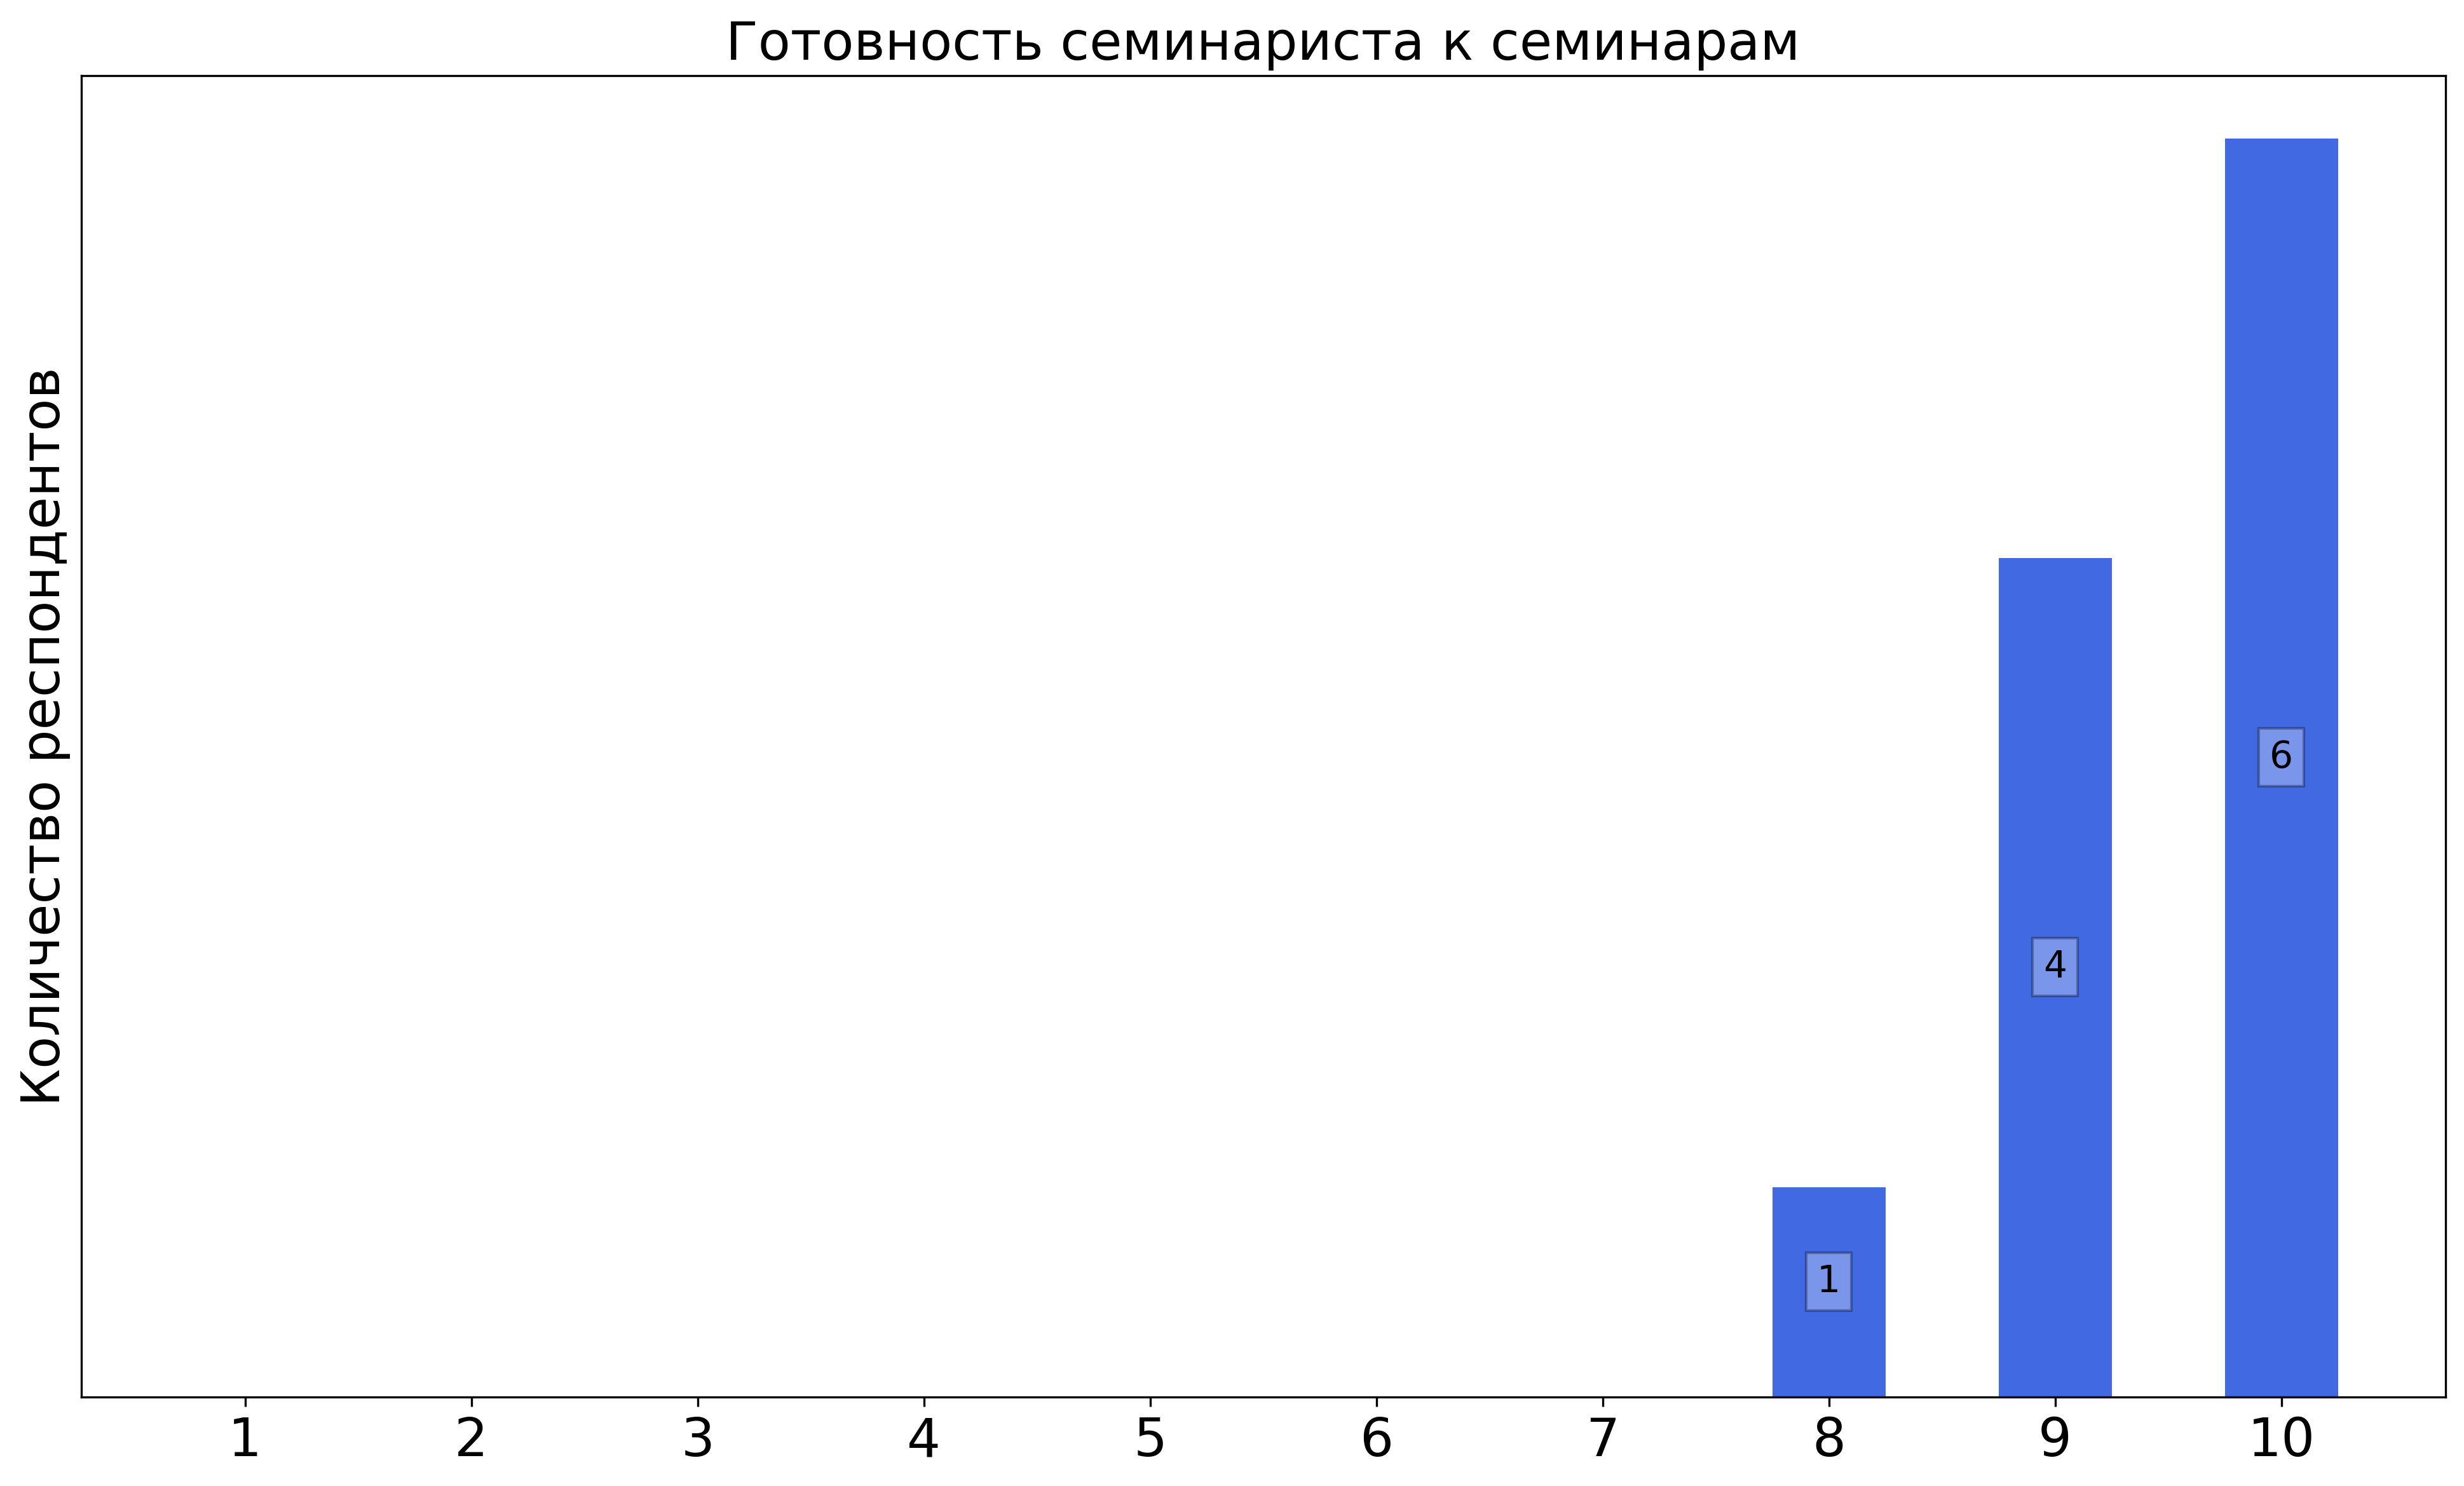
\includegraphics[width=\textwidth]{images/3 course/ТФКП/seminarists-marks-Лопушански М.С.-1.png}
			\end{subfigure}
			\begin{subfigure}[b]{0.45\textwidth}
				\centering
				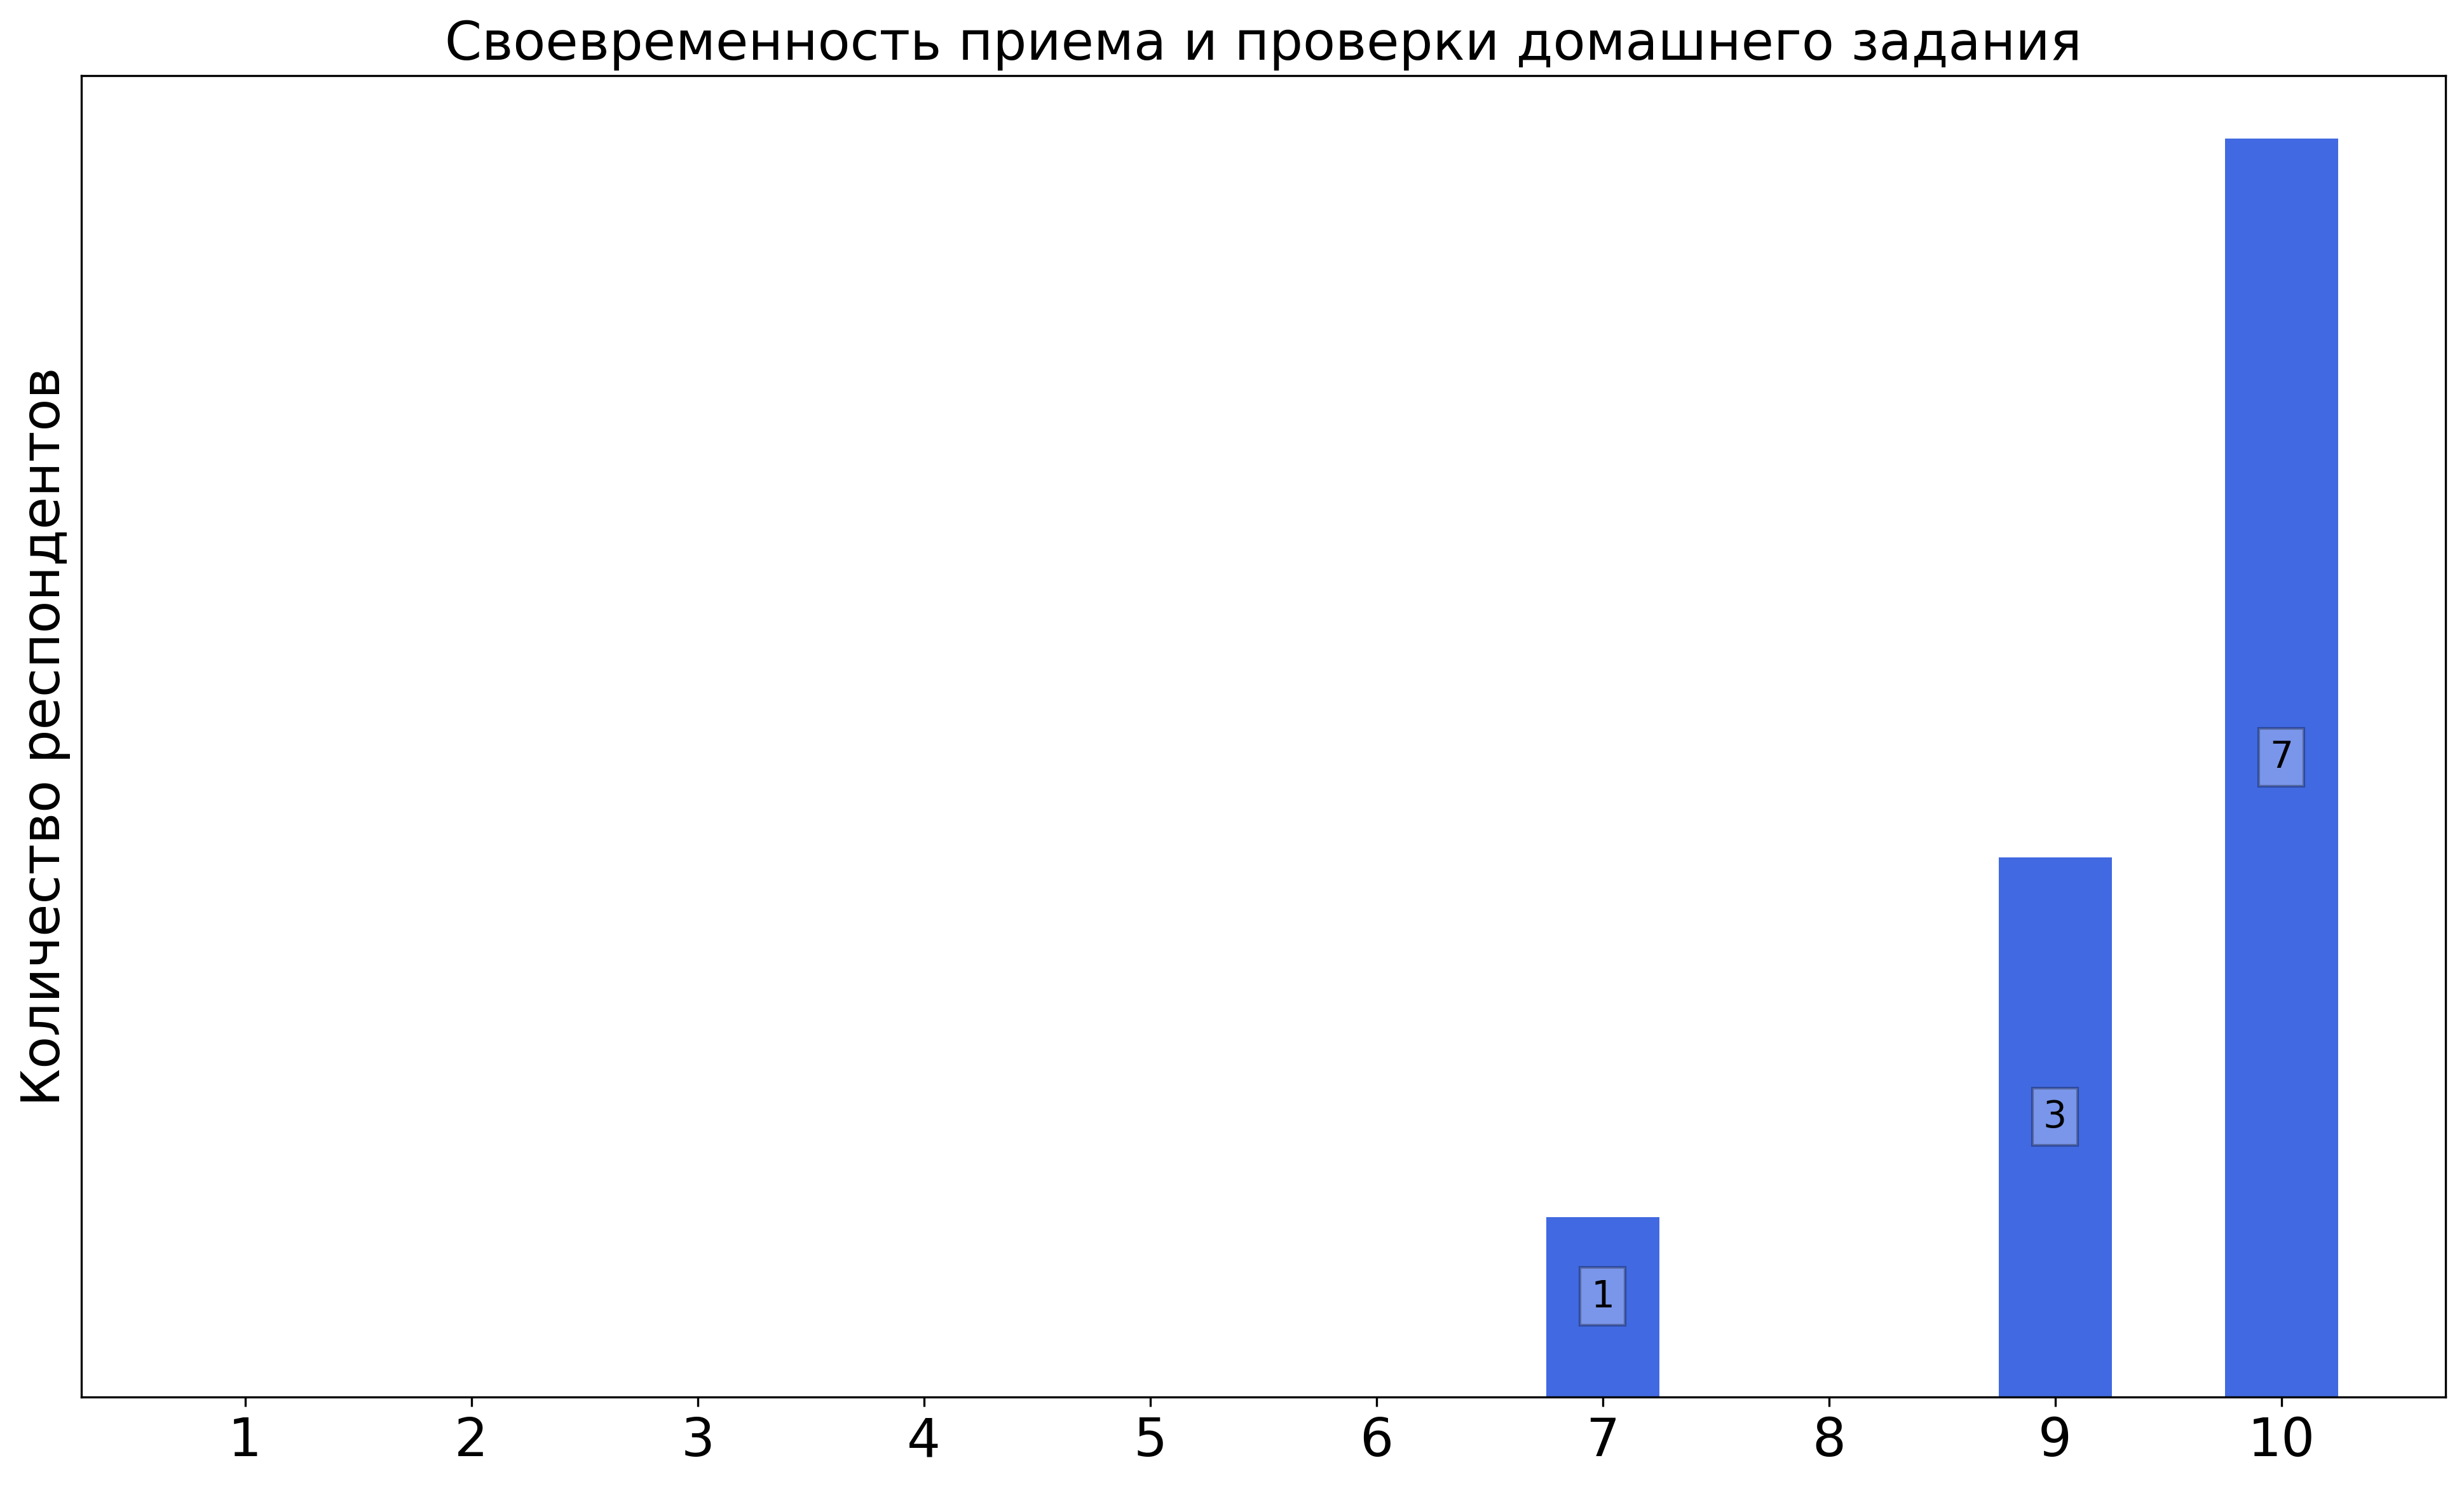
\includegraphics[width=\textwidth]{images/3 course/ТФКП/seminarists-marks-Лопушански М.С.-2.png}
			\end{subfigure}
			\begin{subfigure}[b]{0.45\textwidth}
				\centering
				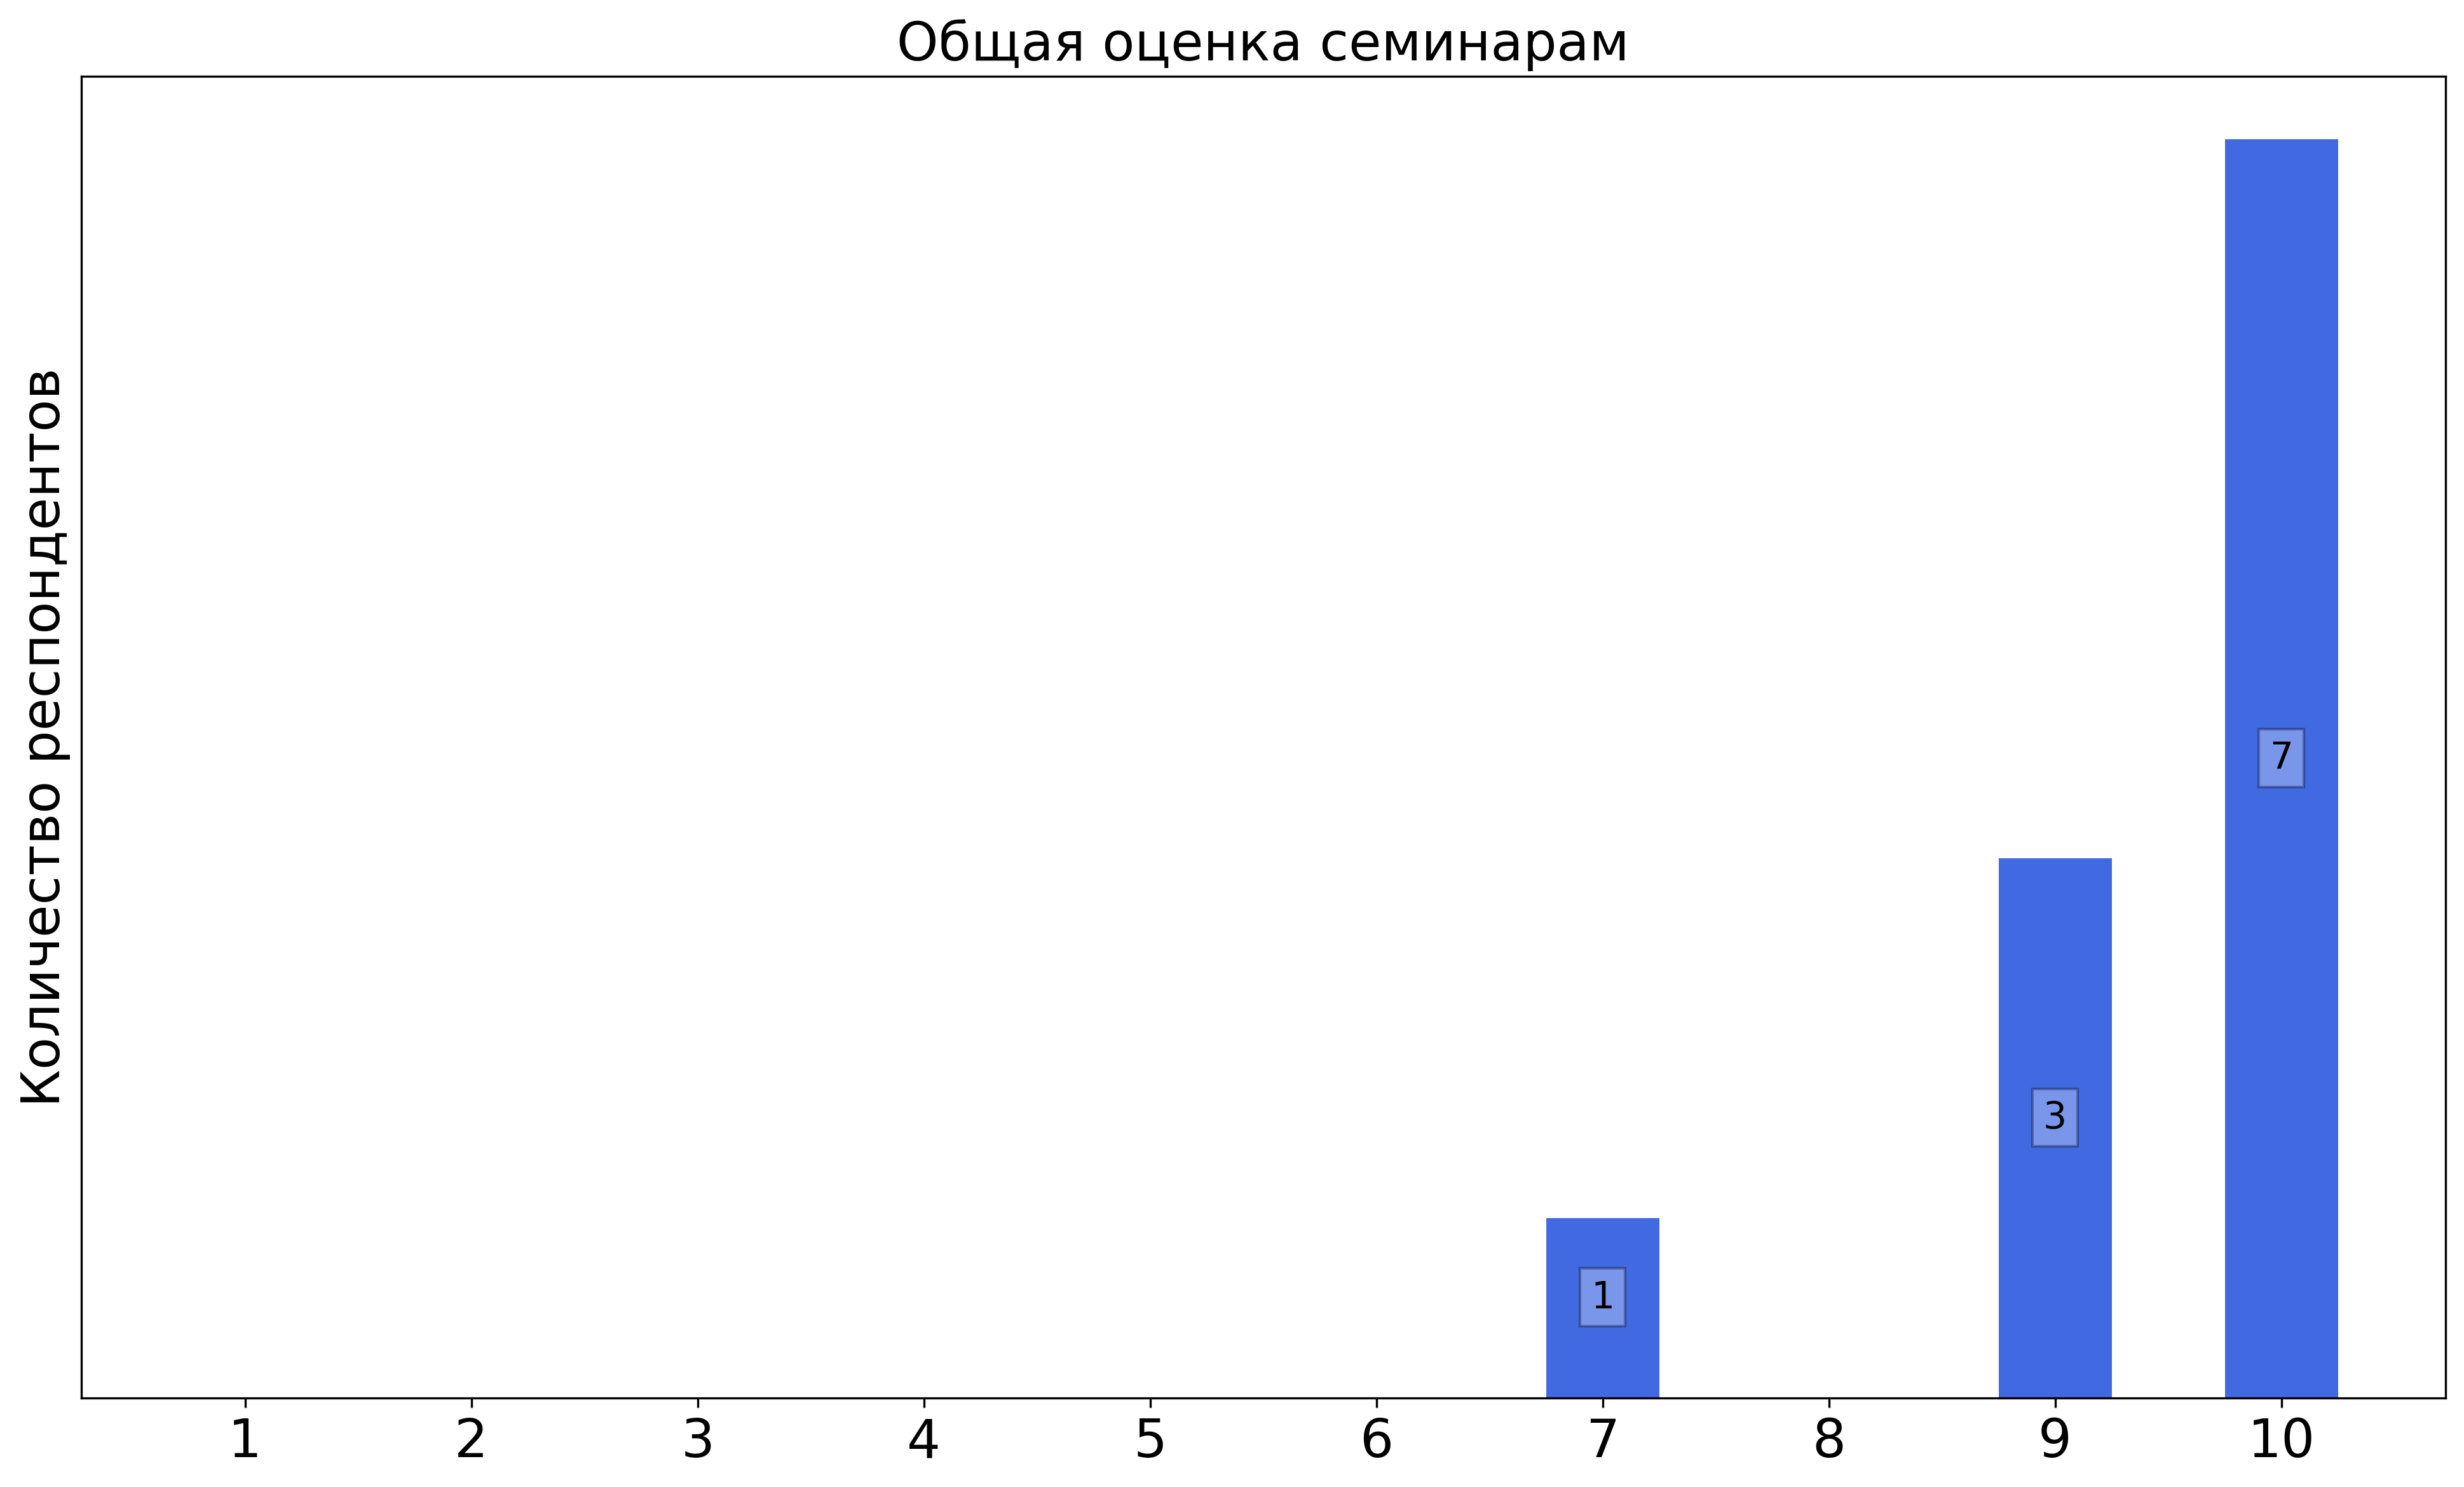
\includegraphics[width=\textwidth]{images/3 course/ТФКП/seminarists-marks-Лопушански М.С.-3.png}
			\end{subfigure}	
			\caption{Оценки респондентов о качестве преподавания семинаров}
		\end{figure}

		\textbf{Комментарии студентов о семинаристе\protect\footnote{сохранены оригинальные орфография и пунктуация}}
            \begin{commentbox} 
                Очень хороший семинарист, на семинарах понятно излагался материал, к системе выставления БРС претензий никогда не возникало. Был на всех семинарах. 
            \end{commentbox} 
        
            \begin{commentbox} 
                Хороший семинарист 
            \end{commentbox} 
        
            \begin{commentbox} 
                Прекрасный семинарист, очень во многом шла на уступки группе, организовывали доп. сдачи, переписывания КР и т.д., объясняет материал тоже понятно 
            \end{commentbox} 


    \subsubsection{Отзыв студентов о семинарах. Семинарист: Самарова С.С.}
		\begin{figure}[H]
			\centering
			\begin{subfigure}[b]{0.45\textwidth}
				\centering
				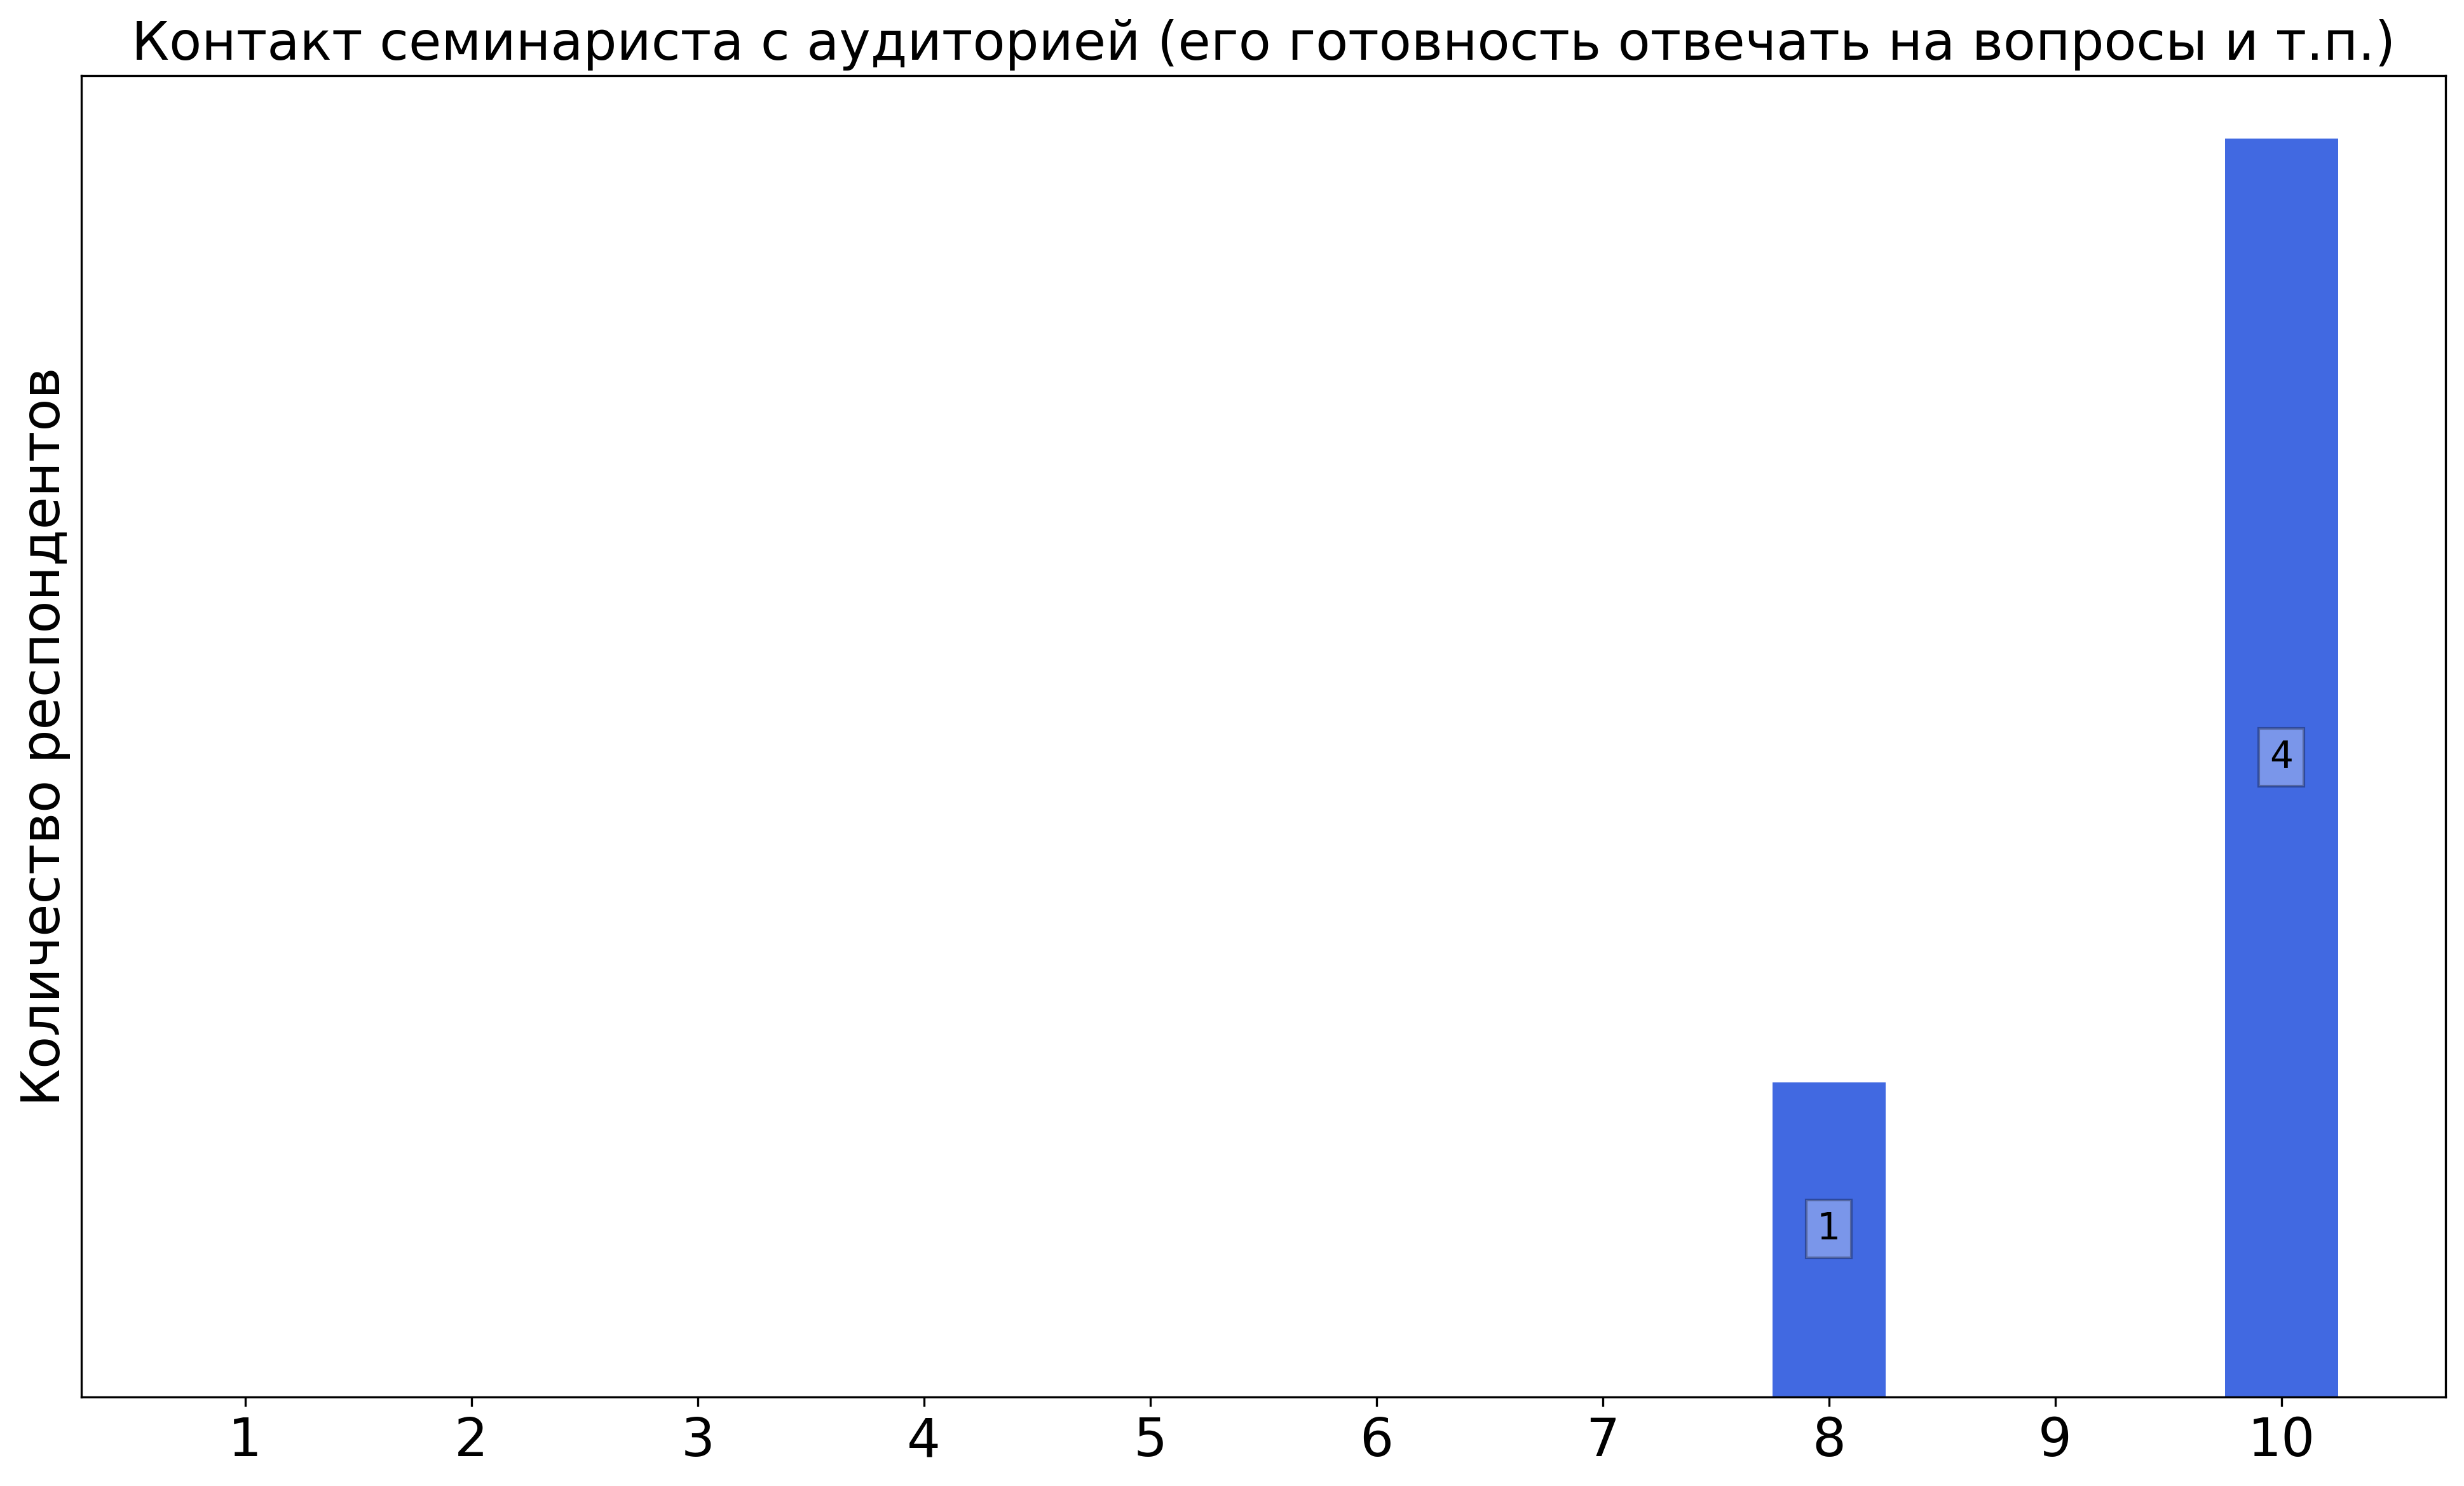
\includegraphics[width=\textwidth]{images/3 course/ТФКП/seminarists-marks-Самарова С.С.-0.png}
			\end{subfigure}
			\begin{subfigure}[b]{0.45\textwidth}
				\centering
				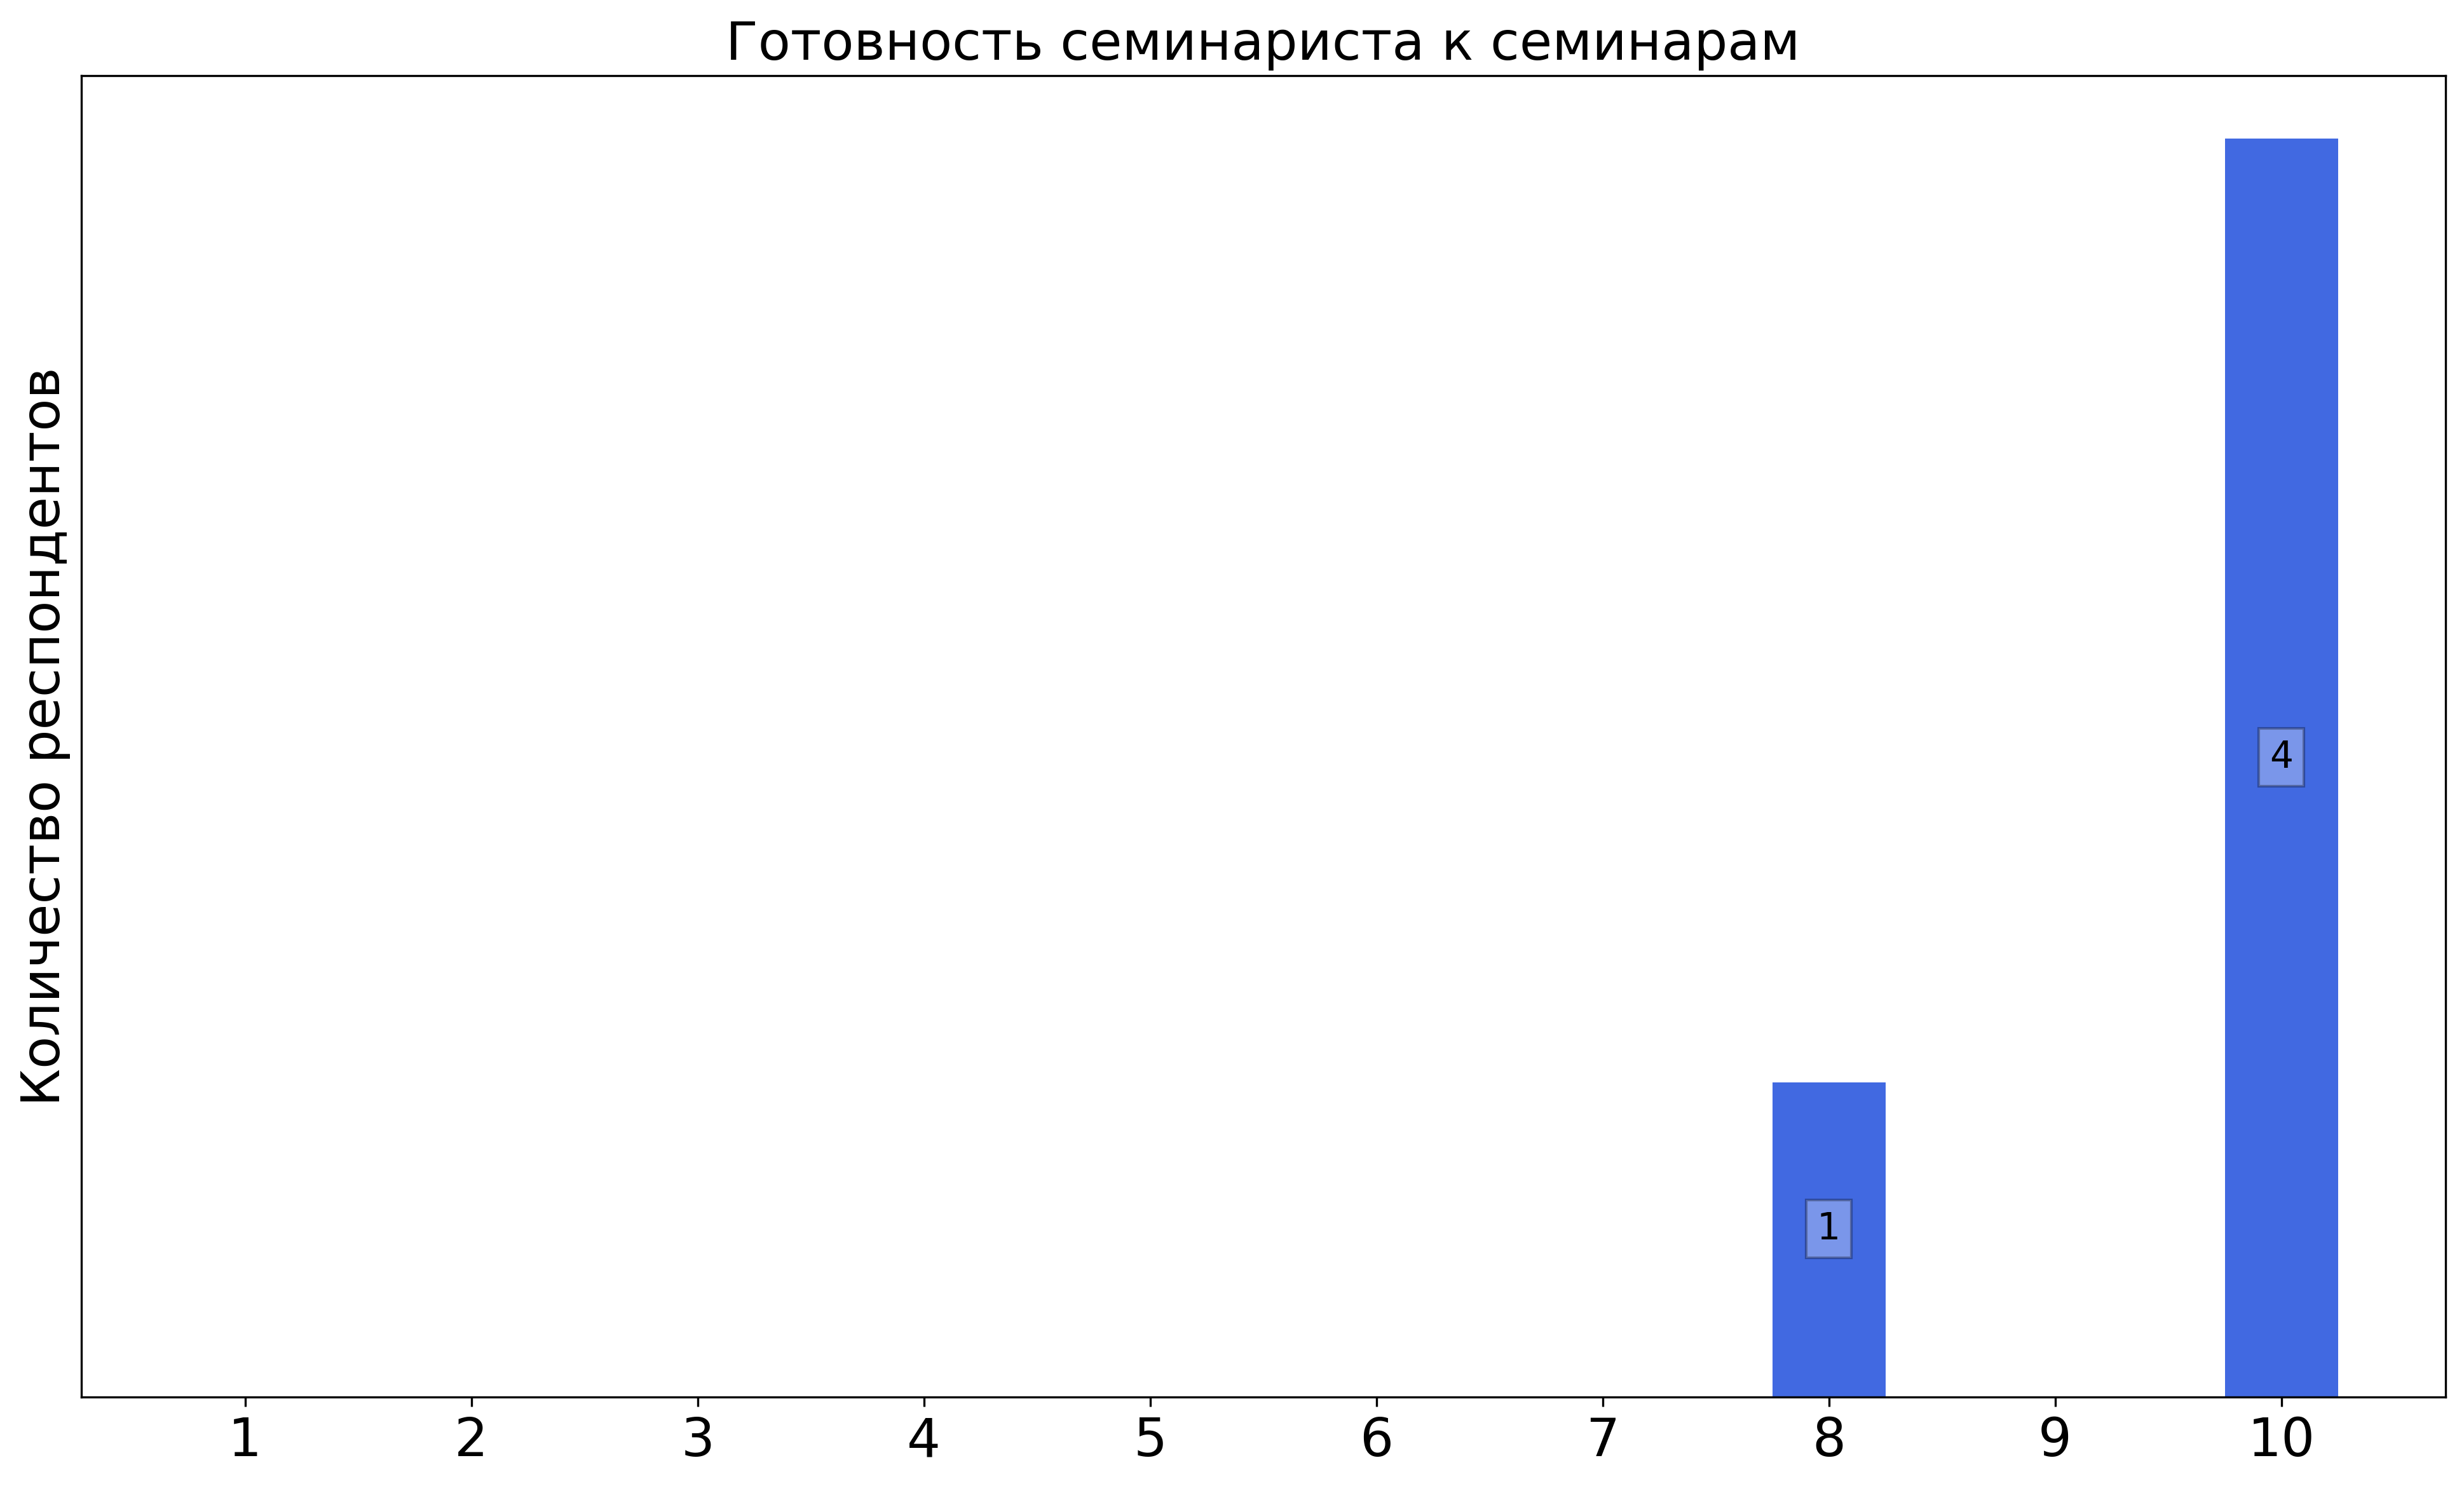
\includegraphics[width=\textwidth]{images/3 course/ТФКП/seminarists-marks-Самарова С.С.-1.png}
			\end{subfigure}
			\begin{subfigure}[b]{0.45\textwidth}
				\centering
				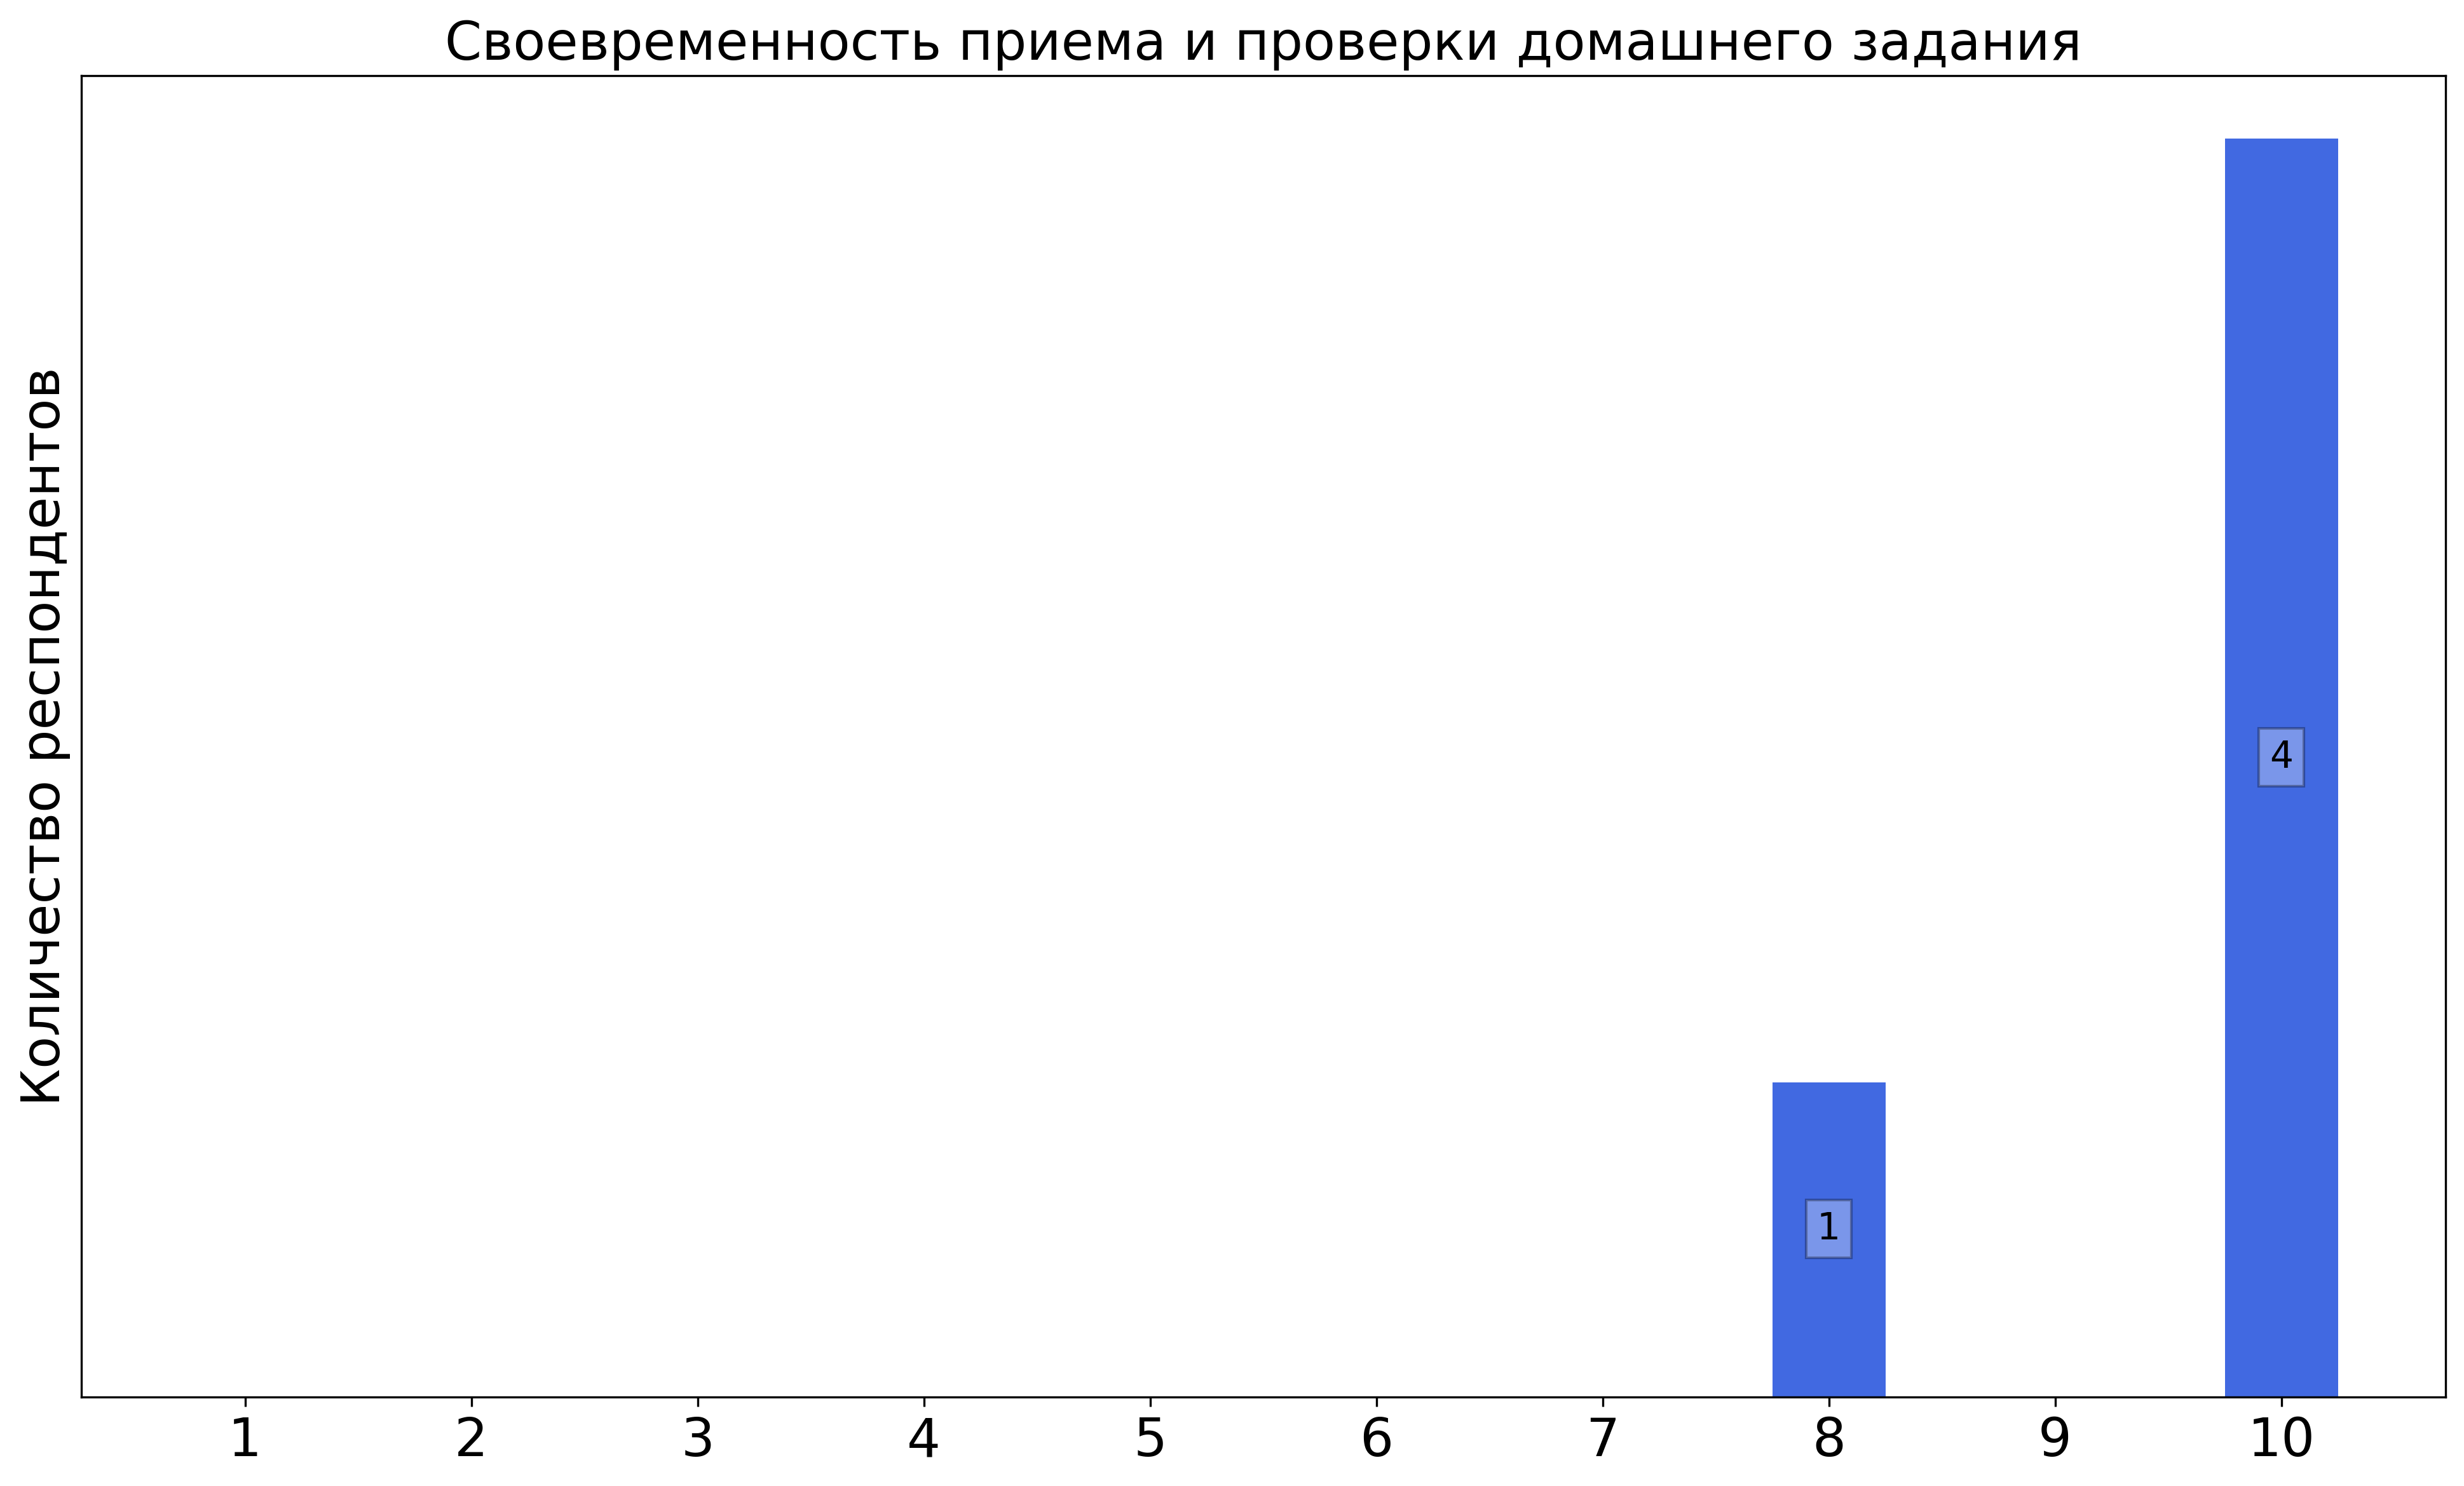
\includegraphics[width=\textwidth]{images/3 course/ТФКП/seminarists-marks-Самарова С.С.-2.png}
			\end{subfigure}
			\begin{subfigure}[b]{0.45\textwidth}
				\centering
				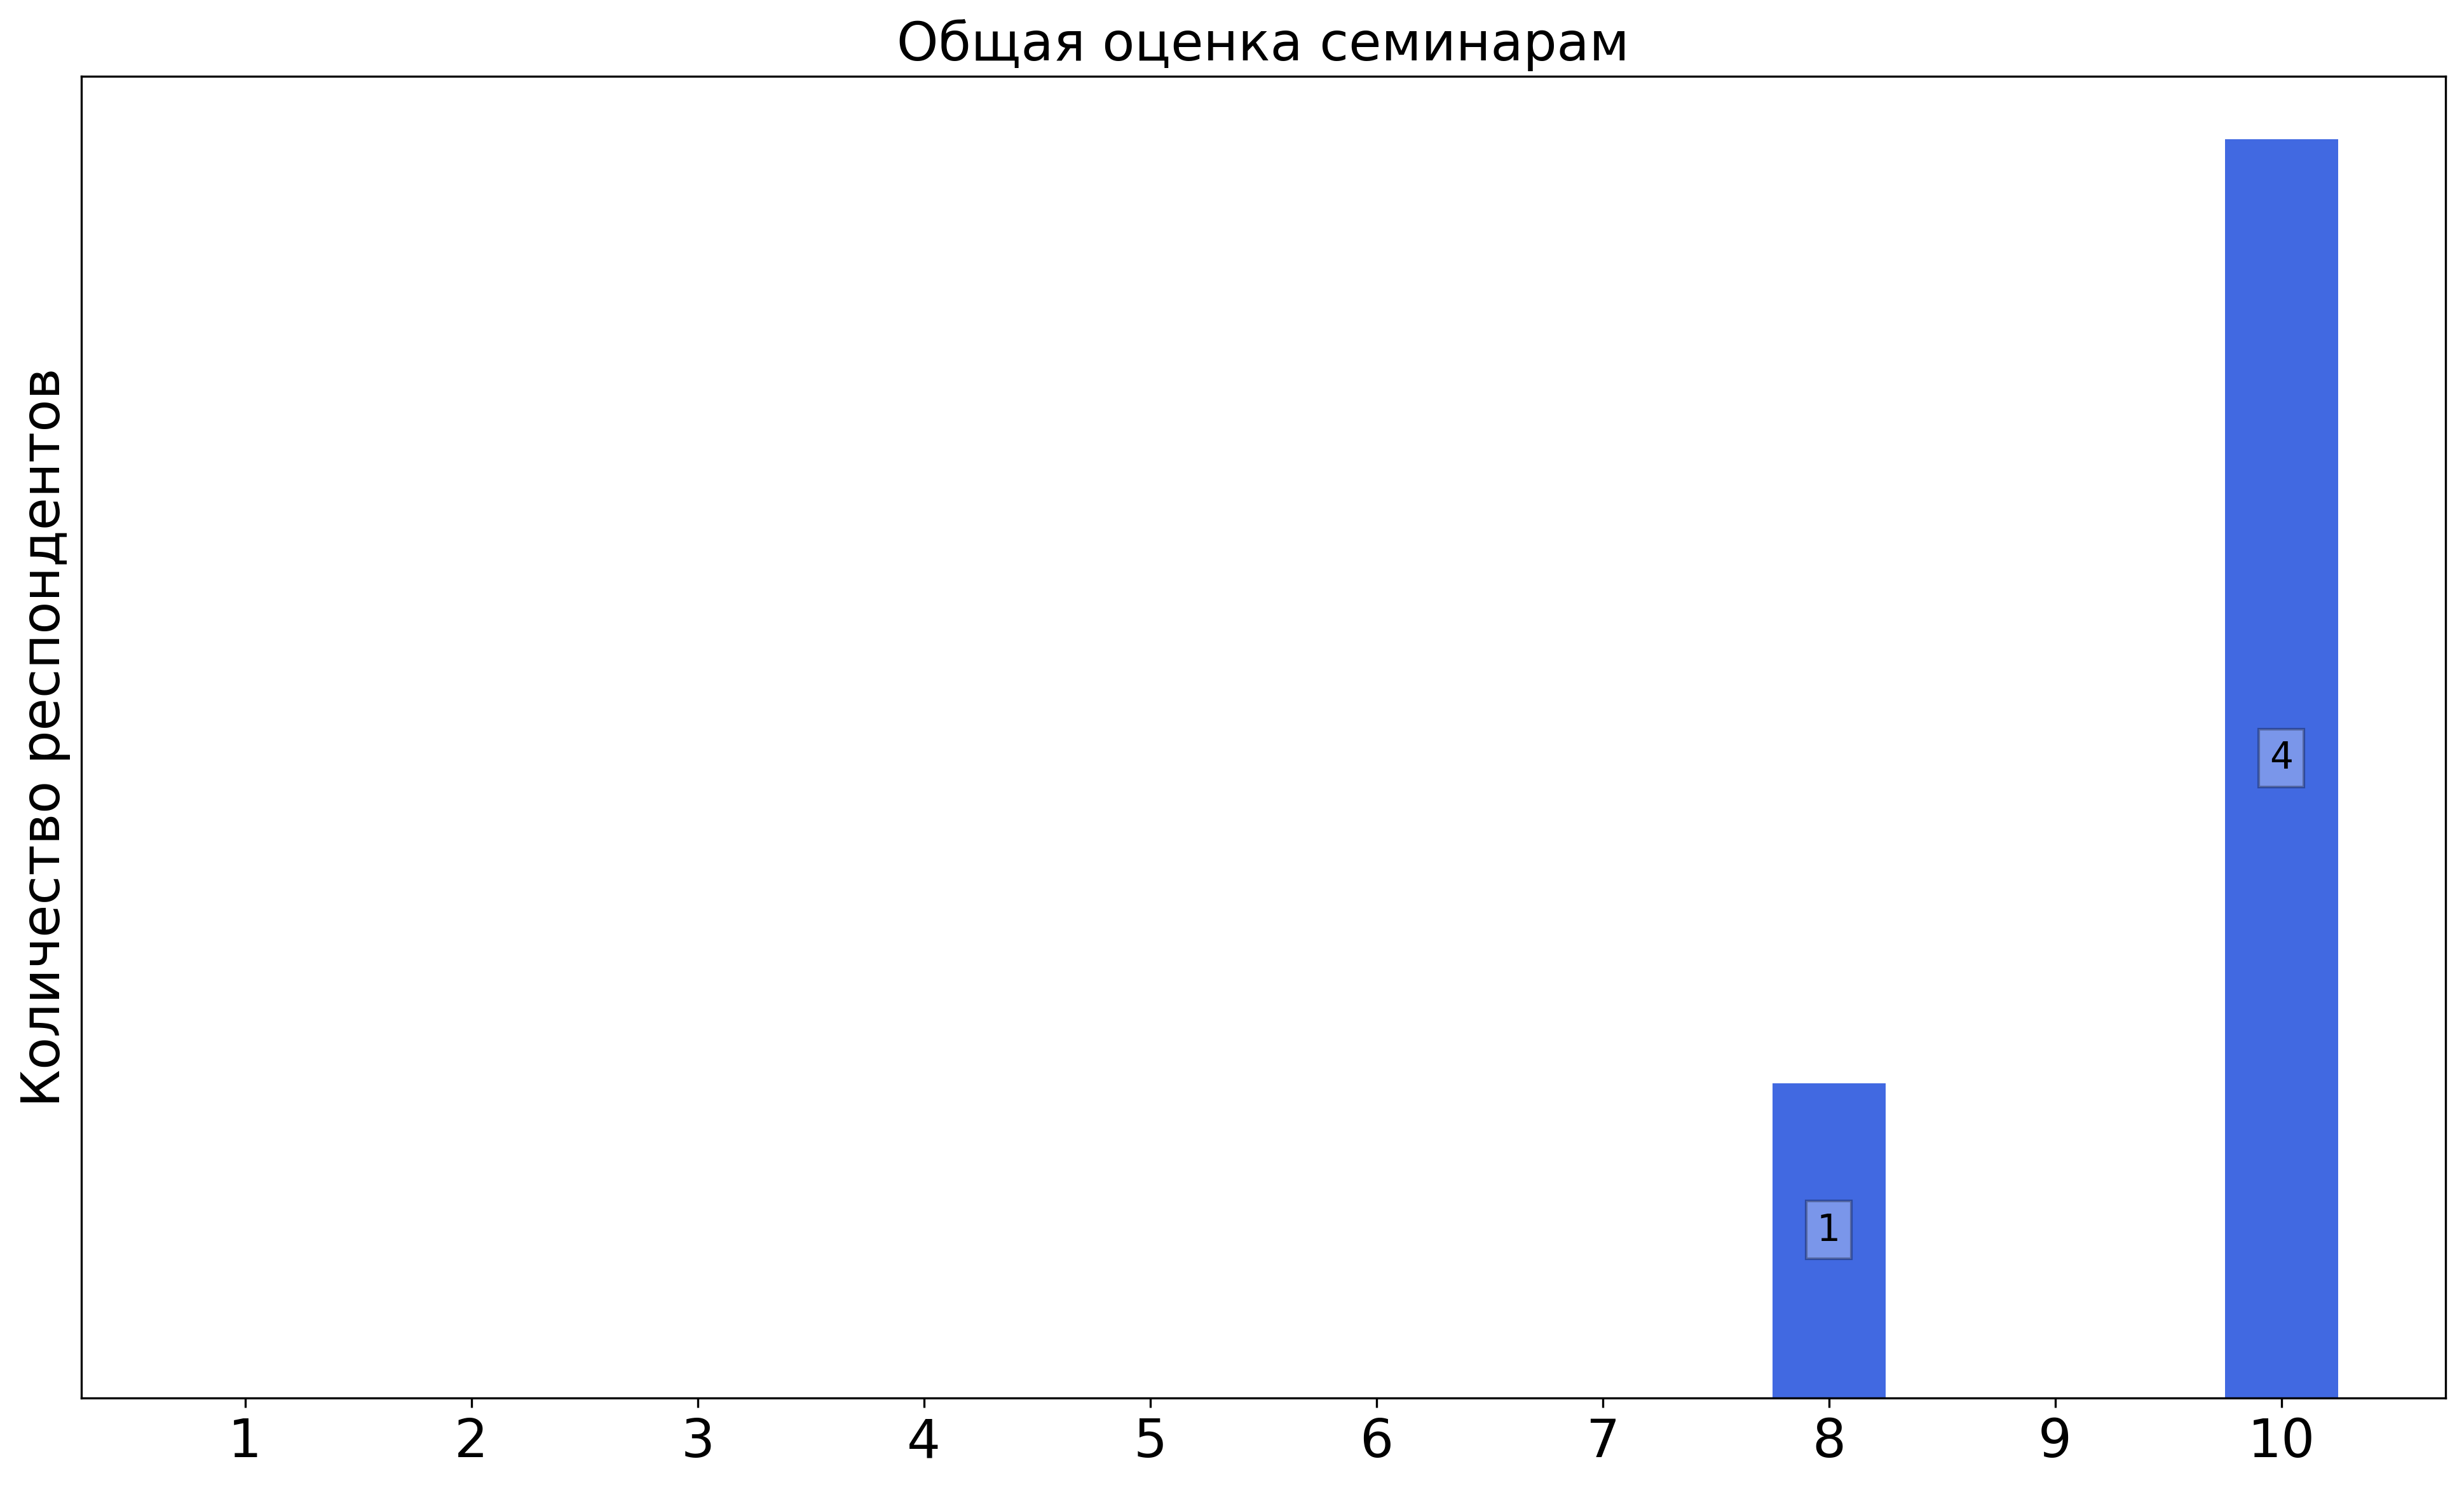
\includegraphics[width=\textwidth]{images/3 course/ТФКП/seminarists-marks-Самарова С.С.-3.png}
			\end{subfigure}	
			\caption{Оценки респондентов о качестве преподавания семинаров}
		\end{figure}

		\textbf{Комментарии студентов о семинаристе\protect\footnote{сохранены оригинальные орфография и пунктуация}}
            \begin{commentbox} 
                Самарова это лучшая семинаристка на свете! 
            \end{commentbox} 
        
            \begin{commentbox} 
                Замечательный семинарист! Отлично объясняла, и получить максимальный БРС при посещении семинаров очень просто. 
            \end{commentbox} 
        
            \begin{commentbox} 
                Самая лучшая женщина на свете. Спасала нас от плохих баллов и во всем старалась идти на встречу студентам. Отвечала даже на самые глупые вопросы студентов 
            \end{commentbox} 


    \subsubsection{Отзыв студентов о семинарах. Семинарист: Филимонов Д.А.}
		\begin{figure}[H]
			\centering
			\begin{subfigure}[b]{0.45\textwidth}
				\centering
				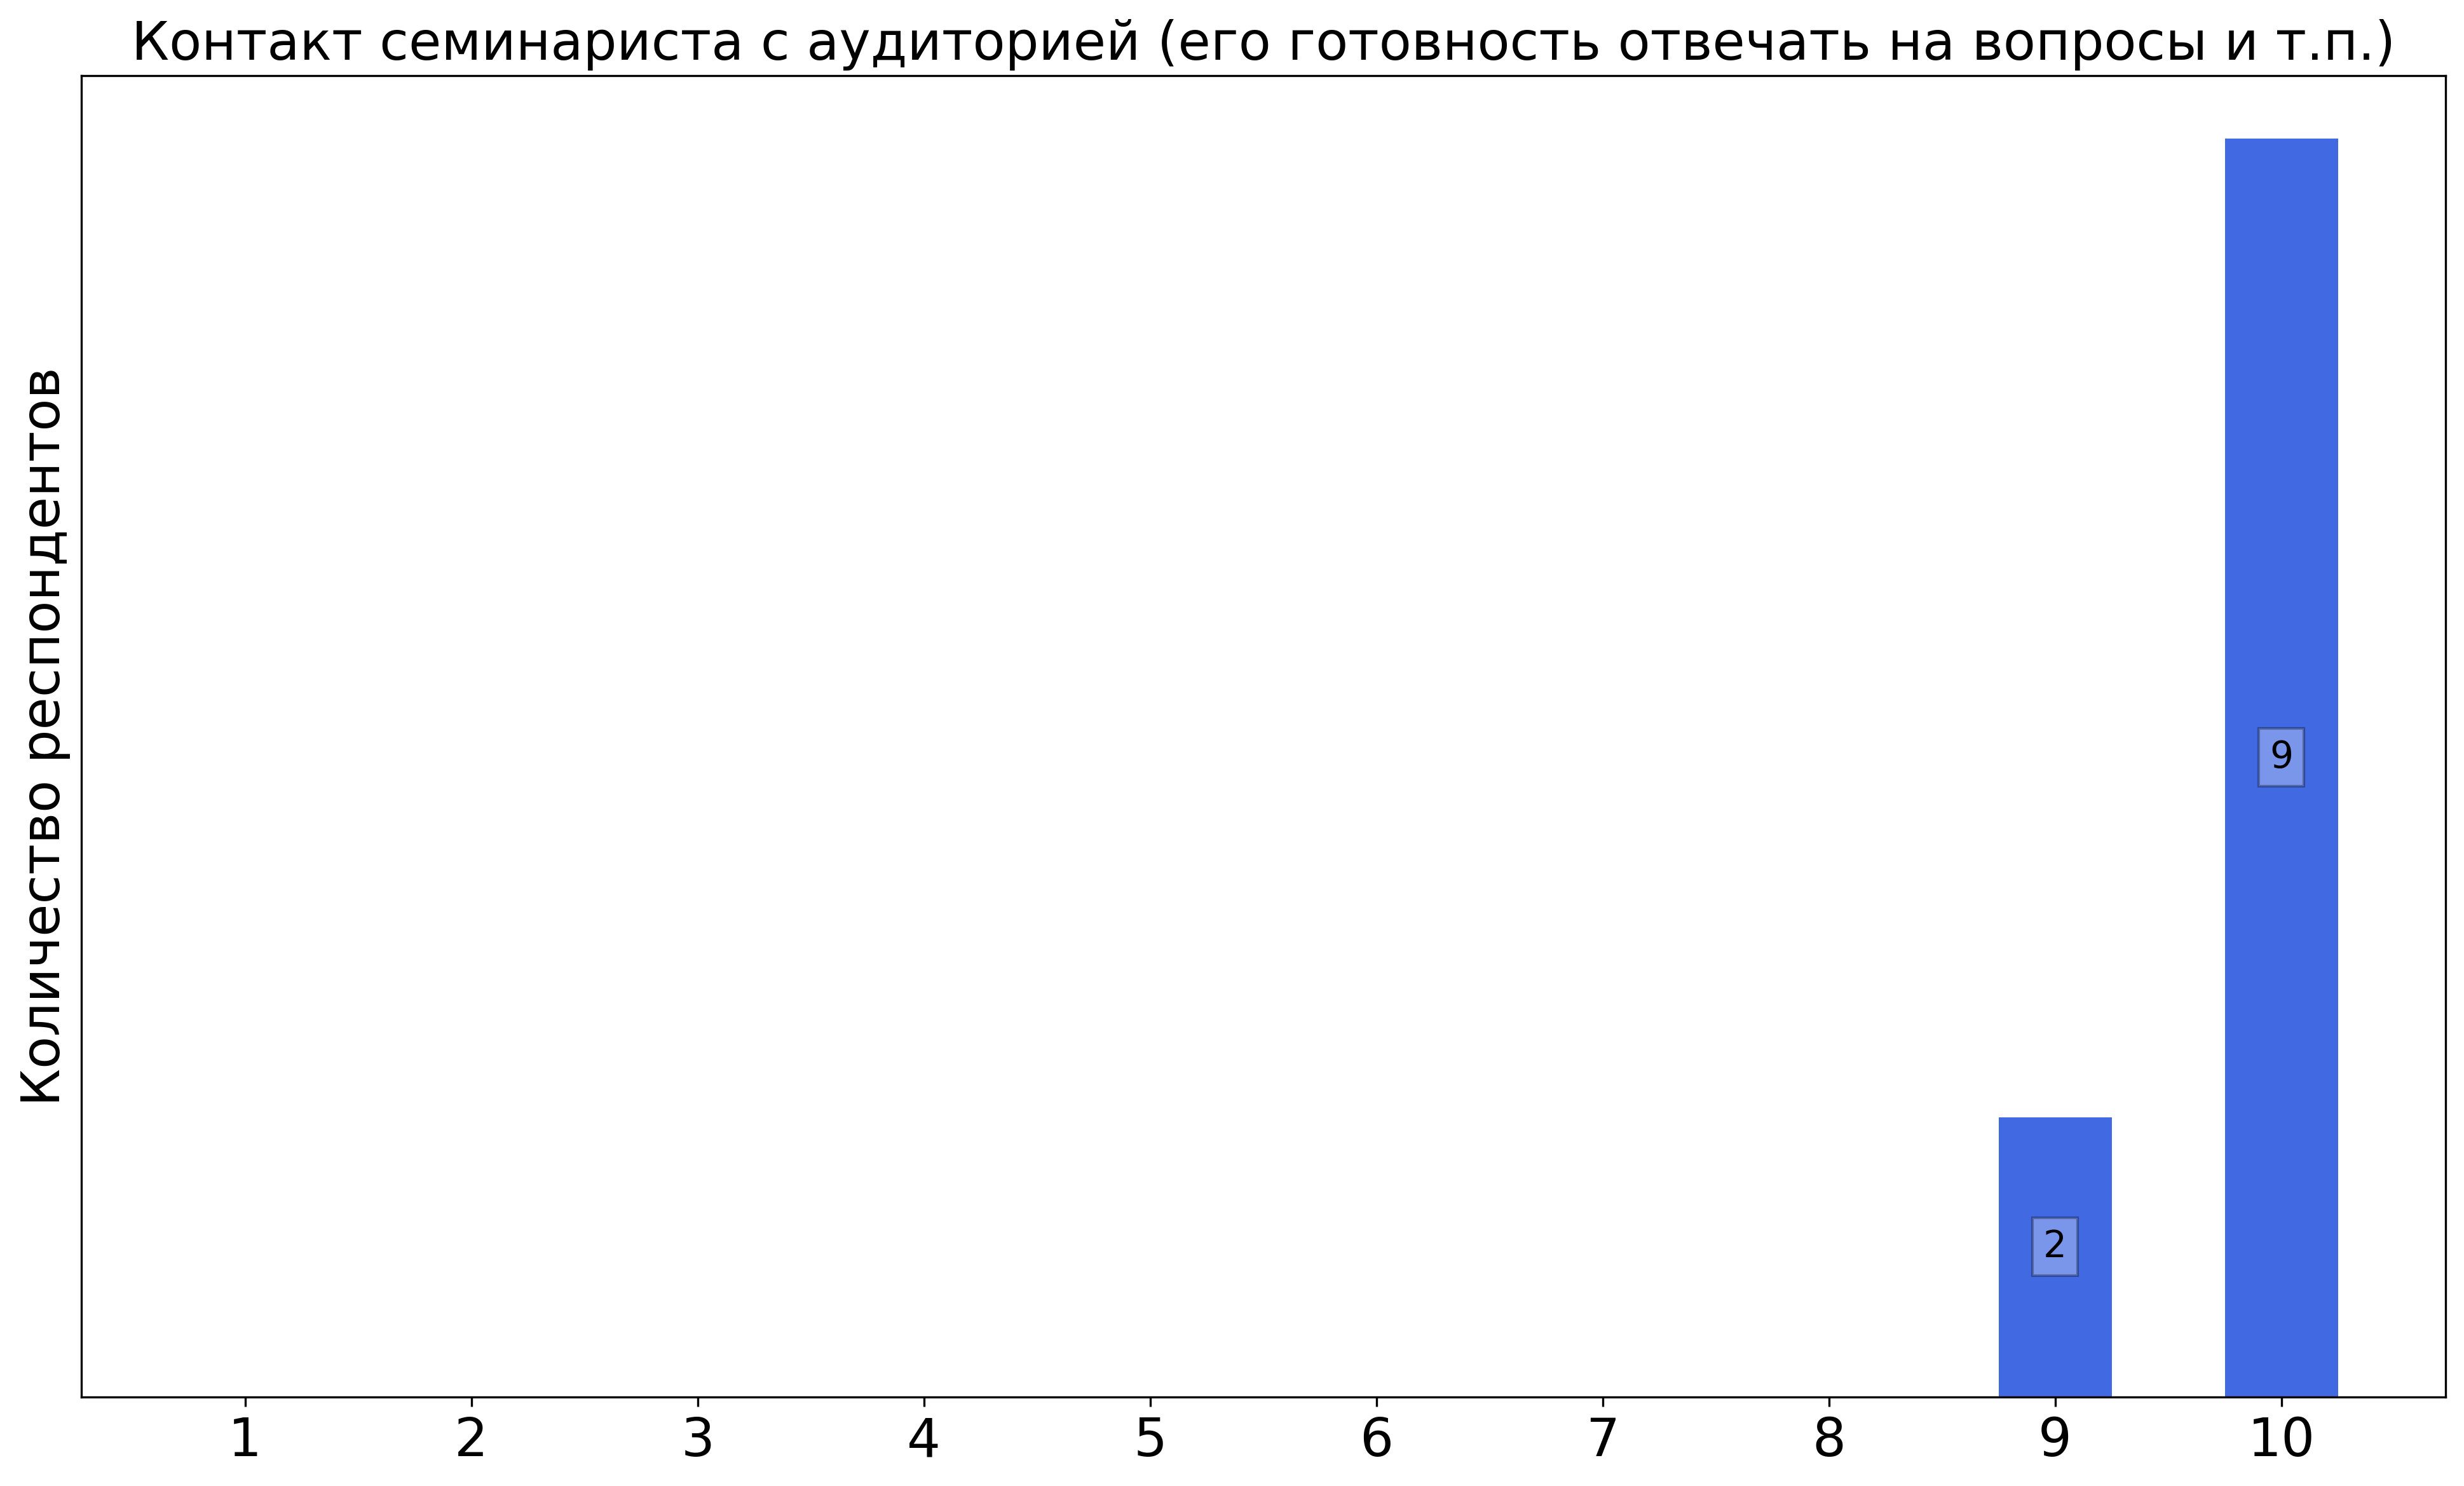
\includegraphics[width=\textwidth]{images/3 course/ТФКП/seminarists-marks-Филимонов Д.А.-0.png}
			\end{subfigure}
			\begin{subfigure}[b]{0.45\textwidth}
				\centering
				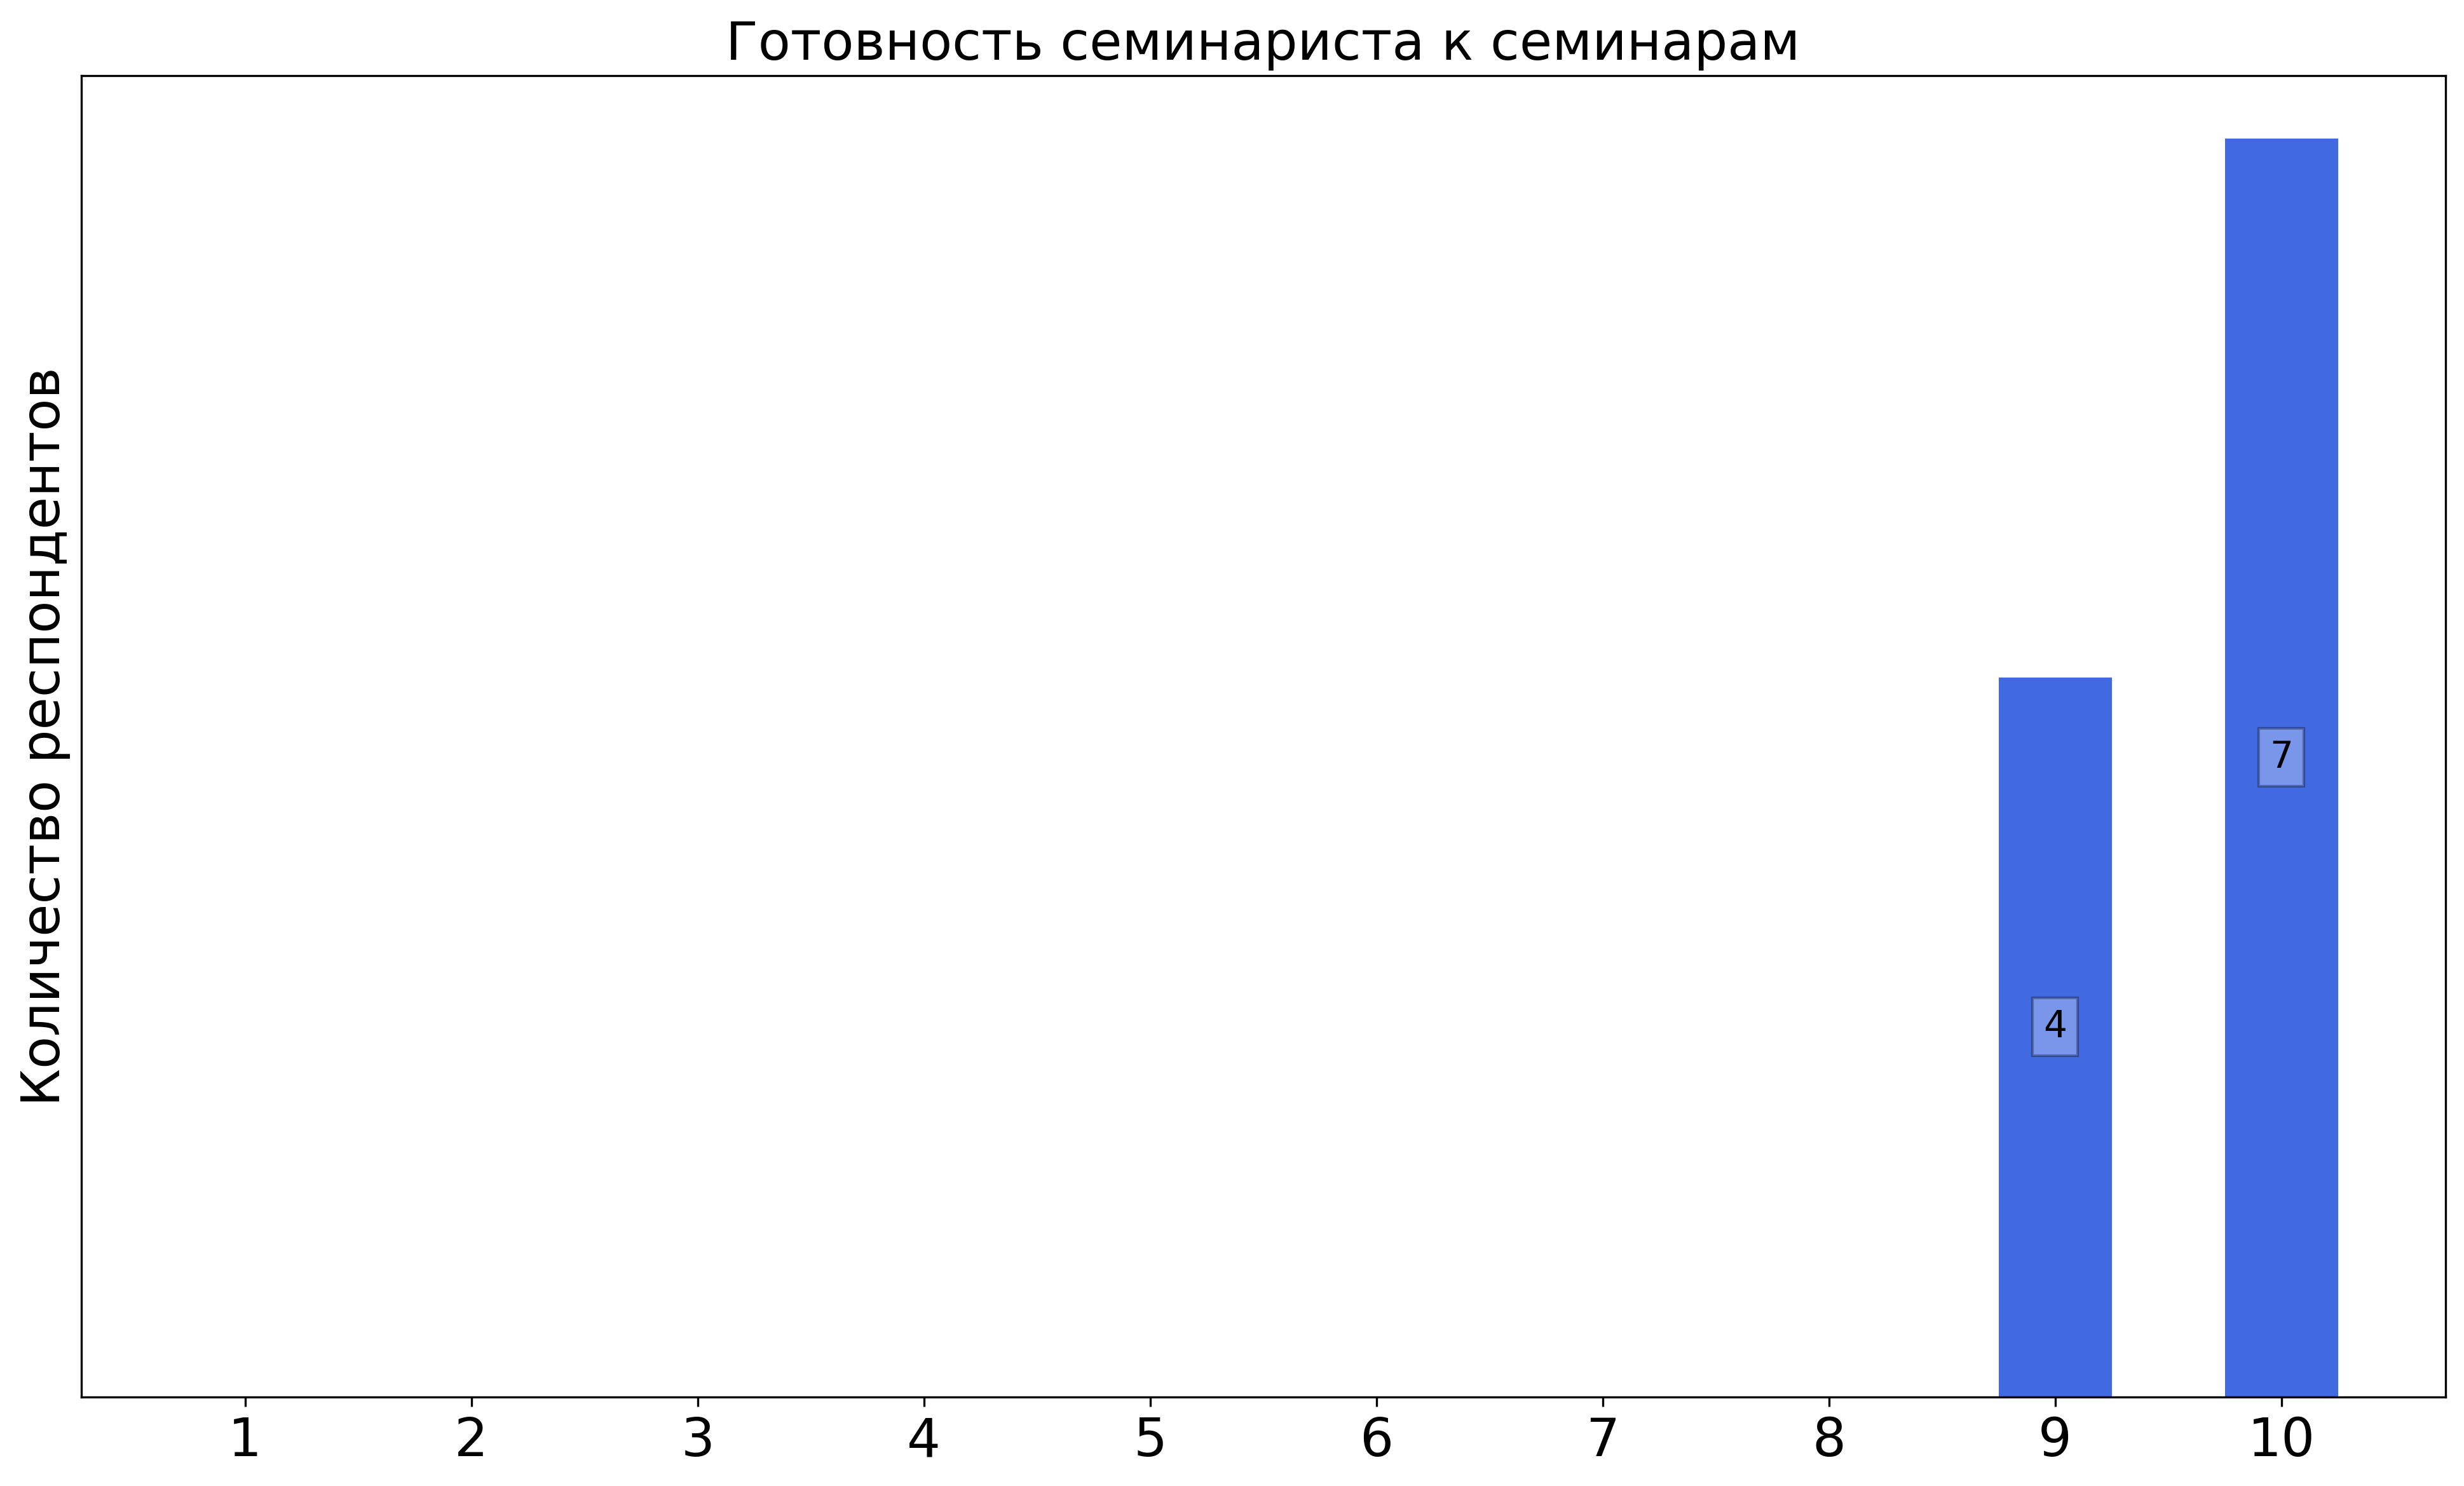
\includegraphics[width=\textwidth]{images/3 course/ТФКП/seminarists-marks-Филимонов Д.А.-1.png}
			\end{subfigure}
			\begin{subfigure}[b]{0.45\textwidth}
				\centering
				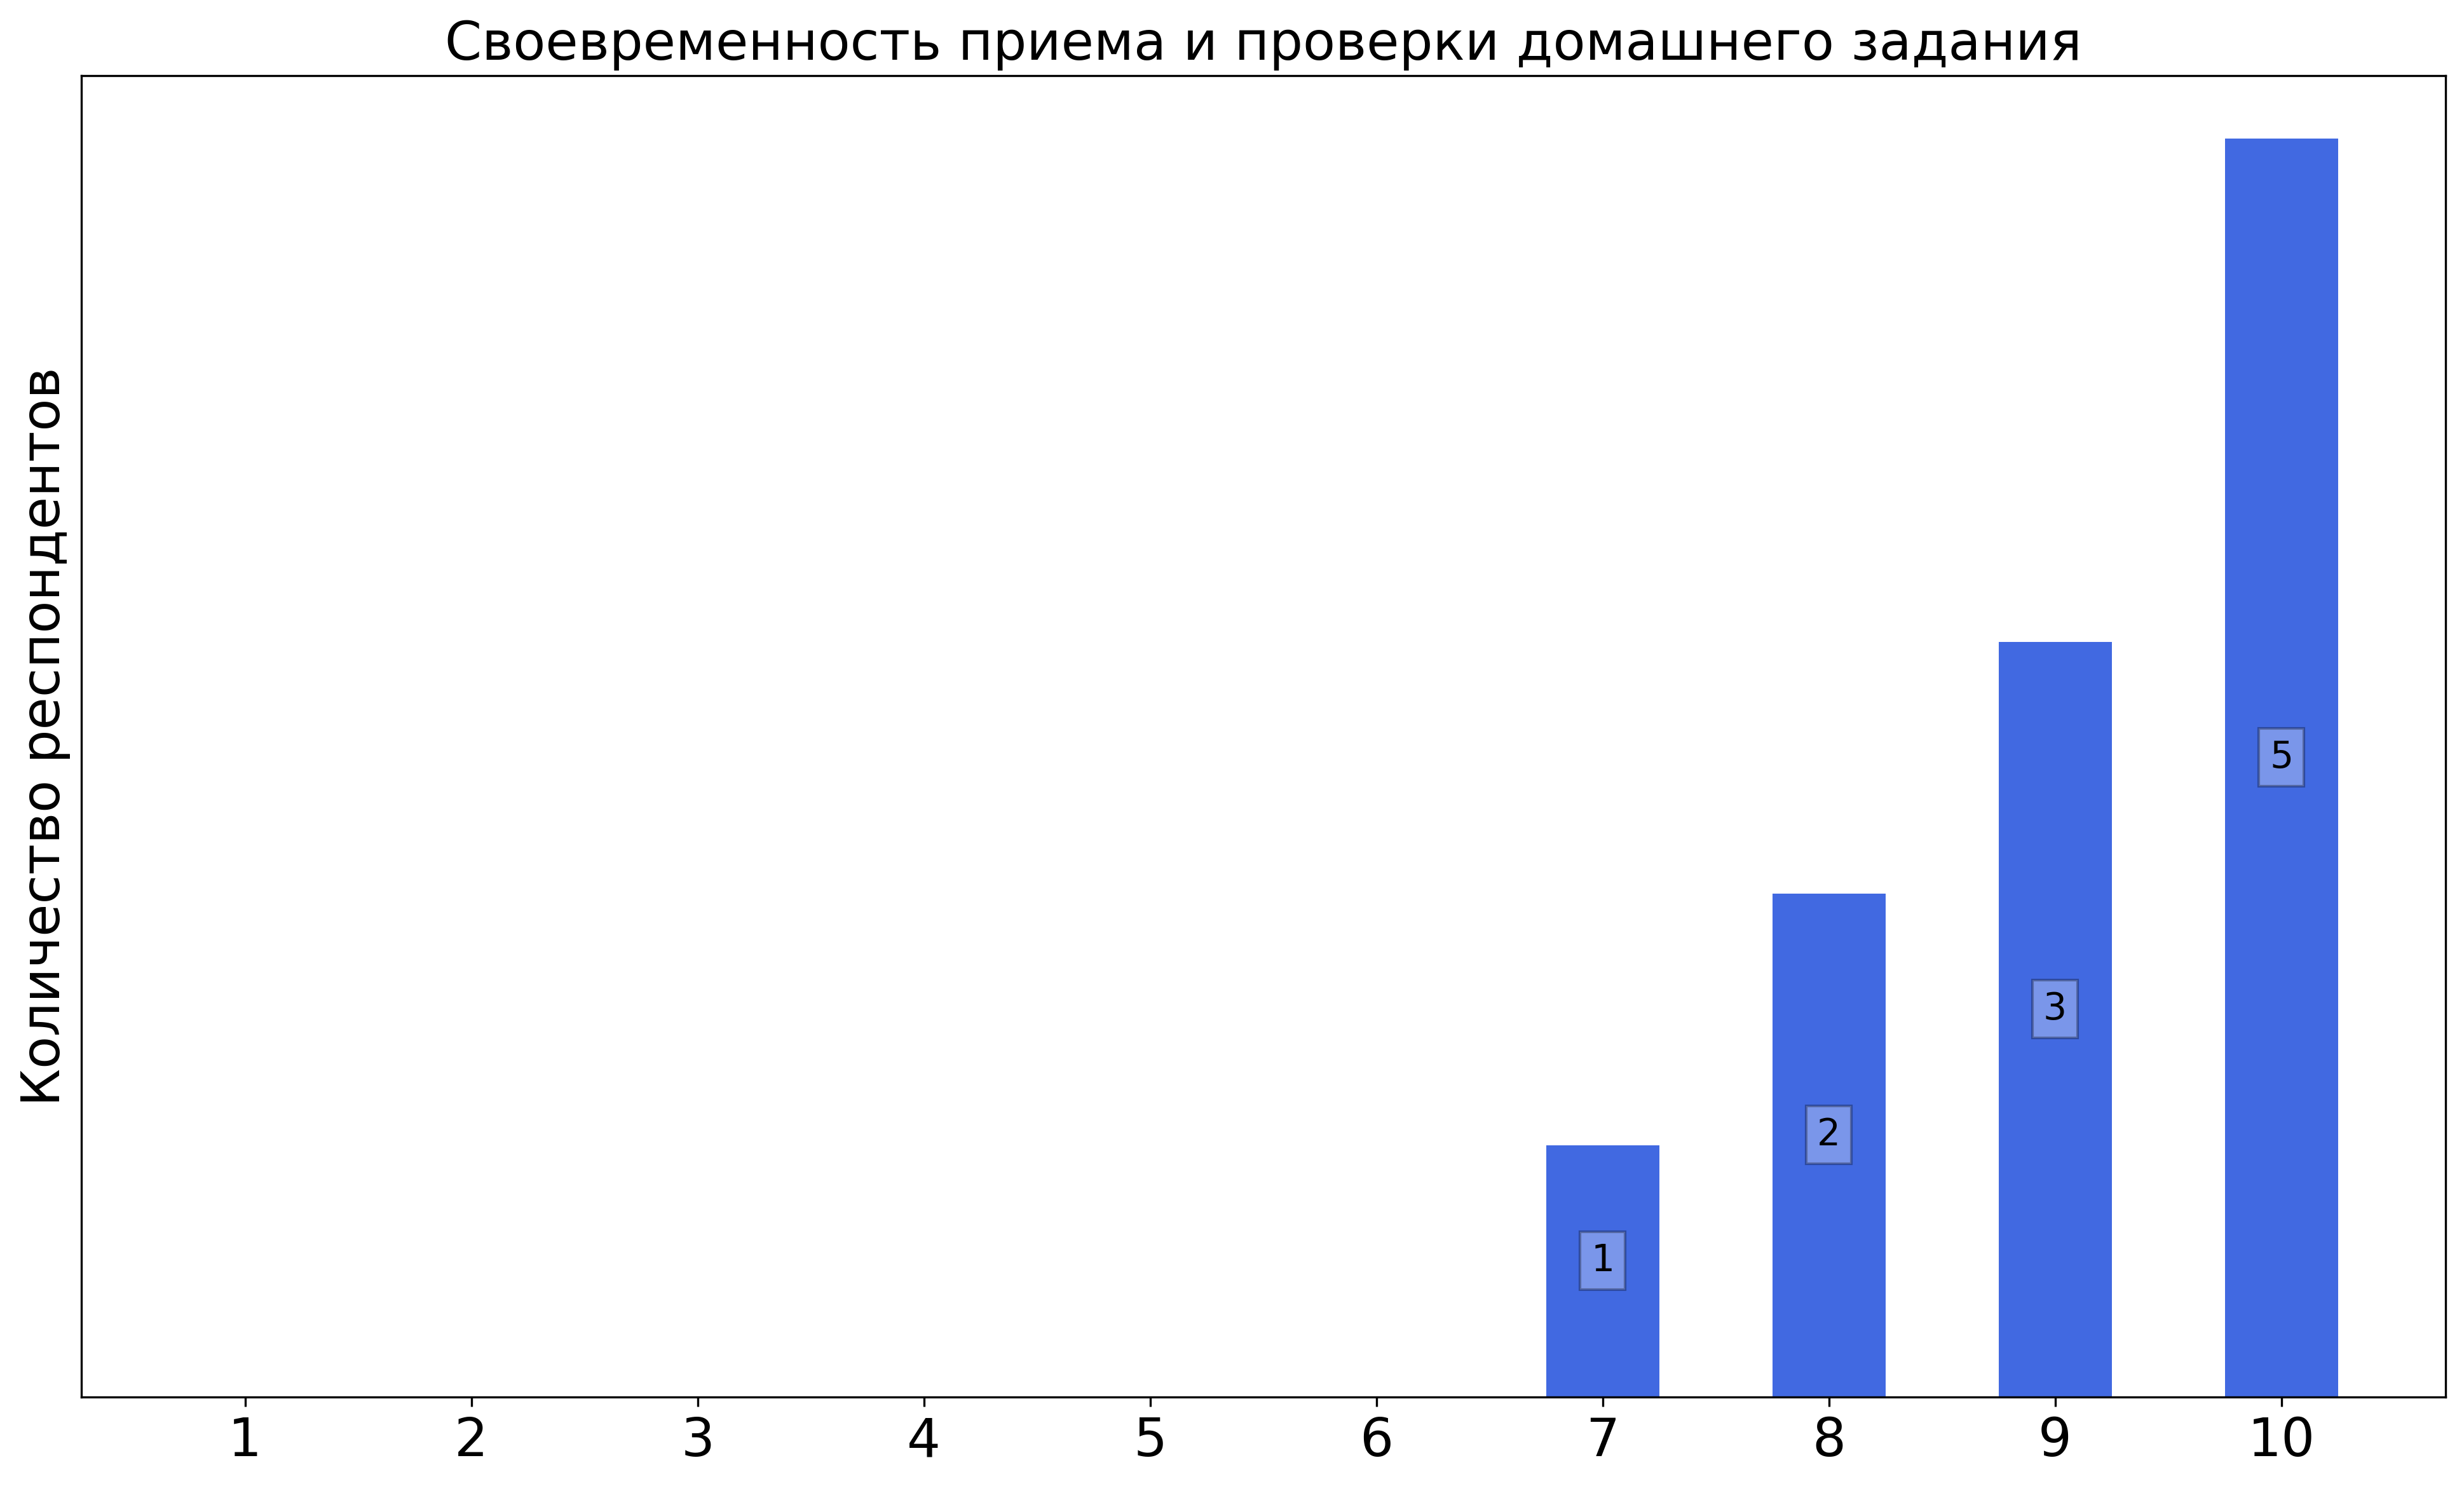
\includegraphics[width=\textwidth]{images/3 course/ТФКП/seminarists-marks-Филимонов Д.А.-2.png}
			\end{subfigure}
			\begin{subfigure}[b]{0.45\textwidth}
				\centering
				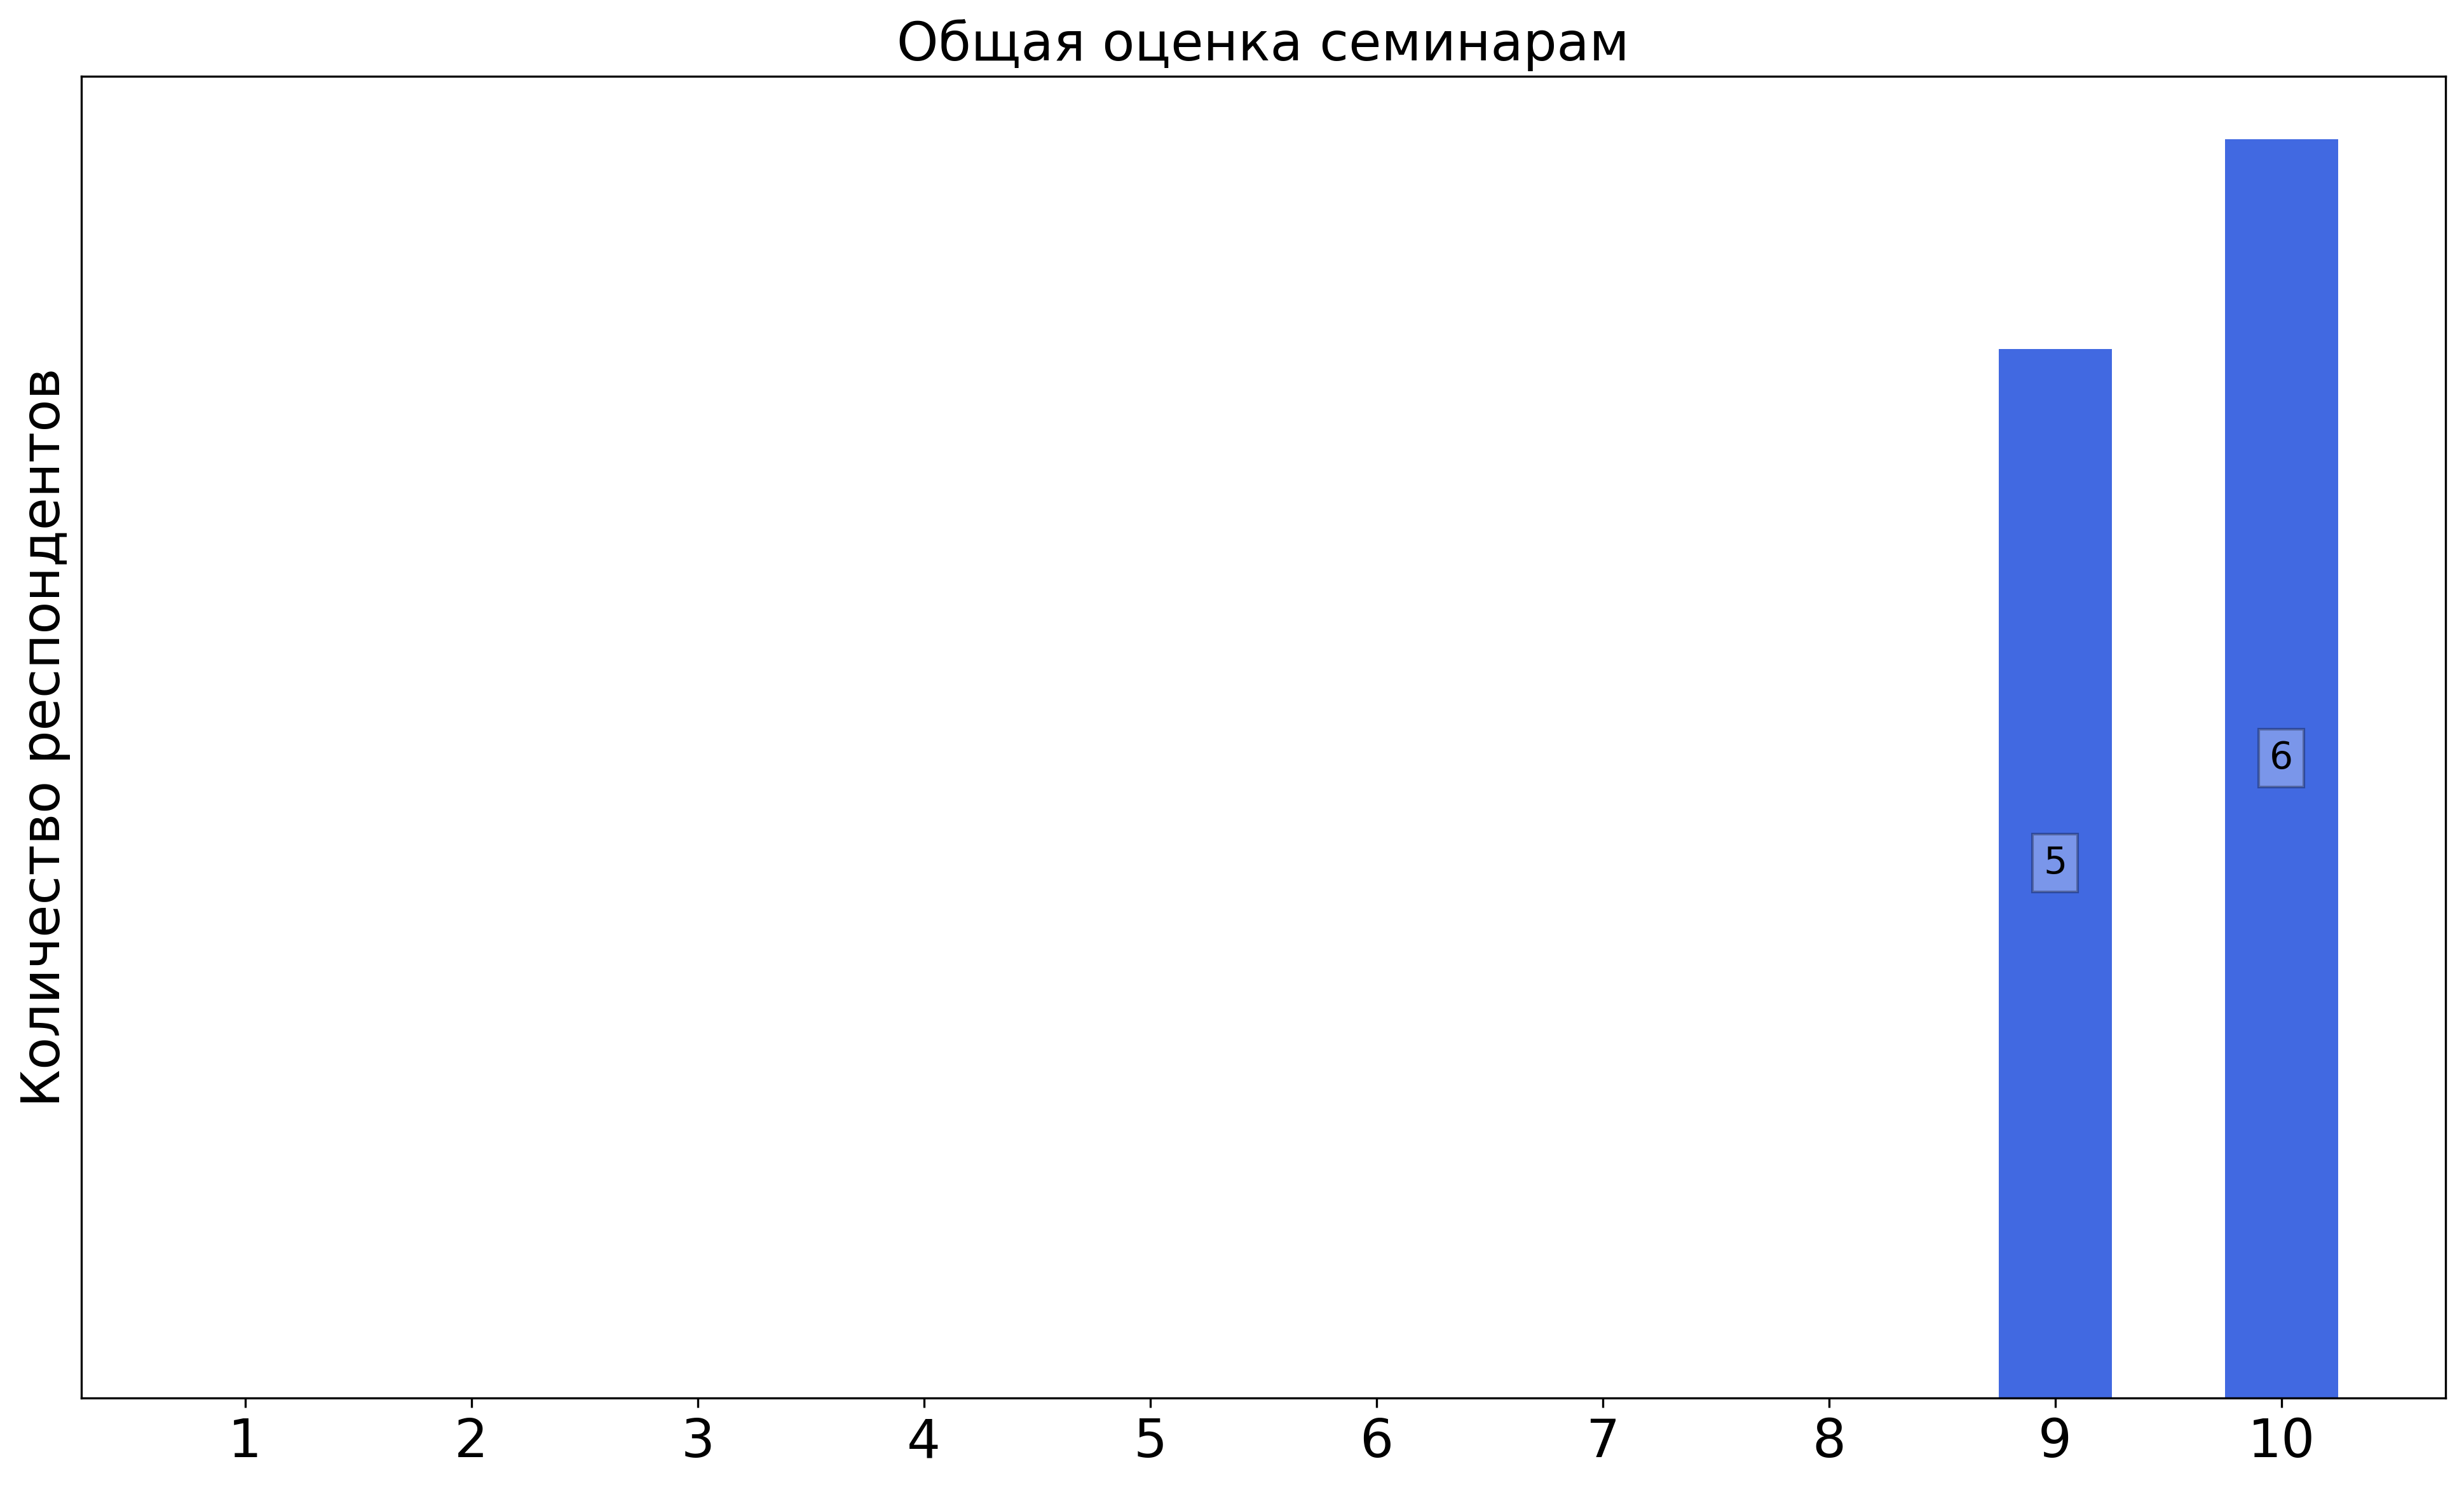
\includegraphics[width=\textwidth]{images/3 course/ТФКП/seminarists-marks-Филимонов Д.А.-3.png}
			\end{subfigure}	
			\caption{Оценки респондентов о качестве преподавания семинаров}
		\end{figure}

		\textbf{Комментарии студентов о семинаристе\protect\footnote{сохранены оригинальные орфография и пунктуация}}
            \begin{commentbox} 
                Очень крутой чувак, сразу видно, что любит свой предмет, хорошо преподает. Это идеальный преподаватель вышмата в моем понимании, так как дает хорошо, но и на экзамене спрашивает жестко 
            \end{commentbox} 
        
            \begin{commentbox} 
                Замечательный семинарист. Это мой первый семестр, когда на семинары кафедры высшей математики ходил с удовольствием. Контрольные работы адекватные по сложности. Можно задать любой вопрос, не бояться, что чего не понимаешь. 
            \end{commentbox} 
        
            \begin{commentbox} 
                Филимонов Д.А. - один из лучших преподавателей, что у меня были. Строгий, добрый, живой и энергичный семинарист, на его семинары почти вся группа весь семестр ходила. 
            \end{commentbox} 
        
            \begin{commentbox} 
                Один из лучших семинаристов на кафедре вышмата 
            \end{commentbox} 
        
            \begin{commentbox} 
                Очень хорошие семинары. Наглядно и понятно объясняется решение задач. Контрольные оптимальной сложности, необходимо прорешивания всего задания для решения. 
            \end{commentbox} 
        
            \begin{commentbox} 
                На семинары хочется ходить, подача материала максимально понятная, рассказано всё по делу и с энтузиазмом, одни из лучших семинаров на кафедре высшей математике лично у меня. 
            \end{commentbox} 

    
    \subsubsection{Прочие комментарии и предложения по улучшению курса}
        \begin{commentbox}
            Не понимаю, какая вообще применимость у некоторых вещей, которые у нас были в курсе, в жизни. Вот как вообще мне нужны конформные преобразования? По ощущениям, это даже в науке нигде толком не используется, я уже молчу про остальные направления 
        \end{commentbox}

        \begin{commentbox}
            С одной стороны жаль, что курс урезанный, с другой, времени на полный нет
        \end{commentbox}

        \begin{commentbox}
            Для курса ТФКП на РТ - самое то
        \end{commentbox}

        \begin{commentbox}
            Сделать курс более обзорным. С наименьшим количеством доказательств, но с наибольшей практической значимостью.
        \end{commentbox}

        \begin{commentbox}
            Убрать из экзамена задачу. Делая семестровую контрольную на 2 задания и тучу контрольных бессмысленно давать задачу на экзамене. Просто вспоминать перед экзаменом требует много времени.
        \end{commentbox}

        \begin{commentbox}
            как обычно, слишком много теории: я понимаю, зачем уметь считать интегралы через вычеты, но не понимаю, зачем знать наизусть и понимать доказательство теоремы, что я могу считать интегралы таким способом
        \end{commentbox}

        \begin{commentbox}
            Часть с конформными отображениями была очень неприятная, но мб это важно знать в будущем (хз, надеюсь что так)
        \end{commentbox}

        \begin{commentbox}
            Было бы чудно если бы была карта курса, где были бы описанны центарльные поятия и теоремы. Что зачем вводится. Хотелось бы больше акцентов на том, как темы связанны с друг другом и где и зачем данная теория применяется. Если бы в курсе были бы задачи приближенные к прикладным, было бы круто
        \end{commentbox}

        \begin{commentbox}
            Как всегда, очень странная и не очень справедливая методика оценивания в виде устного экзамена - единственного момента, когда нужно досконально знать доказательства теорем, при этом этот момент буквально решающий при оценивании на экзамене. Семинарский курс и последовательность изложения материала очень хорошая - одна из лучших за все годы на вышмате, но устный экзамен, как всегда, сильно снижает мнение о предмете и убавляет понимание из-за огромного количества материала, который необходимо удержать в краткосрочной памяти (под пониманием я имею ввиду способность вспомнить материал условно через год, уверен, без 5 дневного бота теории, не нужной в практических приложениях, полезной информации о методах решения отложилось бы больше)
        \end{commentbox}

        \begin{commentbox}
            Пожелания, скорее, касаются любого предмета кафедры высшей математики, а не конкретно ТФКП. Хотелось бы, чтобы курс был менее теоретическим, и упор ставился именно на прикладной аспект. В большей степени это касается лекций и экзамена по предмету, так как, на мой взгляд, в заучивании доказательств теорем никакого смысла нет. Лучше бы на лекциях вместо длинных доказательств теорем было больше пояснений того, как их применять, и экзамены строились на каких-то примерах/контрпримерах, а не в заучивании большого количества материала, не имеющего никакого отношения к практике, или и вовсе были полностью заменены уже существующими письменными экзаменами/семестровыми контрольными (в случае ТФКП).
        \end{commentbox}

        \begin{commentbox}
            Лучше синхронизировать материалы лекций и программу экзаменов.
        \end{commentbox}

        \begin{commentbox}
            Курс хороший, многие теоретические моменты отличаются у разных лекторов, у Бунакова часто не очень строгие, но понятные доказательства. Смотрел в записи
        \end{commentbox}

        \begin{commentbox}
            Хотелось бы более "живые" семинары, с большим количеством задач, без потери времени на их поиск.
        \end{commentbox}